\documentclass[twoside]{book}

% Packages required by doxygen
\usepackage{fixltx2e}
\usepackage{calc}
\usepackage{doxygen}
\usepackage[export]{adjustbox} % also loads graphicx
\usepackage{graphicx}
\usepackage[utf8]{inputenc}
\usepackage{makeidx}
\usepackage{multicol}
\usepackage{multirow}
\PassOptionsToPackage{warn}{textcomp}
\usepackage{textcomp}
\usepackage[nointegrals]{wasysym}
\usepackage[table]{xcolor}

% Font selection
\usepackage[T1]{fontenc}
\usepackage[scaled=.90]{helvet}
\usepackage{courier}
\usepackage{amssymb}
\usepackage{sectsty}
\renewcommand{\familydefault}{\sfdefault}
\allsectionsfont{%
  \fontseries{bc}\selectfont%
  \color{darkgray}%
}
\renewcommand{\DoxyLabelFont}{%
  \fontseries{bc}\selectfont%
  \color{darkgray}%
}
\newcommand{\+}{\discretionary{\mbox{\scriptsize$\hookleftarrow$}}{}{}}

% Page & text layout
\usepackage{geometry}
\geometry{%
  a4paper,%
  top=2.5cm,%
  bottom=2.5cm,%
  left=2.5cm,%
  right=2.5cm%
}
\tolerance=750
\hfuzz=15pt
\hbadness=750
\setlength{\emergencystretch}{15pt}
\setlength{\parindent}{0cm}
\setlength{\parskip}{3ex plus 2ex minus 2ex}
\makeatletter
\renewcommand{\paragraph}{%
  \@startsection{paragraph}{4}{0ex}{-1.0ex}{1.0ex}{%
    \normalfont\normalsize\bfseries\SS@parafont%
  }%
}
\renewcommand{\subparagraph}{%
  \@startsection{subparagraph}{5}{0ex}{-1.0ex}{1.0ex}{%
    \normalfont\normalsize\bfseries\SS@subparafont%
  }%
}
\makeatother

% Headers & footers
\usepackage{fancyhdr}
\pagestyle{fancyplain}
\fancyhead[LE]{\fancyplain{}{\bfseries\thepage}}
\fancyhead[CE]{\fancyplain{}{}}
\fancyhead[RE]{\fancyplain{}{\bfseries\leftmark}}
\fancyhead[LO]{\fancyplain{}{\bfseries\rightmark}}
\fancyhead[CO]{\fancyplain{}{}}
\fancyhead[RO]{\fancyplain{}{\bfseries\thepage}}
\fancyfoot[LE]{\fancyplain{}{}}
\fancyfoot[CE]{\fancyplain{}{}}
\fancyfoot[RE]{\fancyplain{}{\bfseries\scriptsize Generated by Doxygen }}
\fancyfoot[LO]{\fancyplain{}{\bfseries\scriptsize Generated by Doxygen }}
\fancyfoot[CO]{\fancyplain{}{}}
\fancyfoot[RO]{\fancyplain{}{}}
\renewcommand{\footrulewidth}{0.4pt}
\renewcommand{\chaptermark}[1]{%
  \markboth{#1}{}%
}
\renewcommand{\sectionmark}[1]{%
  \markright{\thesection\ #1}%
}

% Indices & bibliography
\usepackage{natbib}
\usepackage[titles]{tocloft}
\setcounter{tocdepth}{3}
\setcounter{secnumdepth}{5}
\makeindex

% Hyperlinks (required, but should be loaded last)
\usepackage{ifpdf}
\ifpdf
  \usepackage[pdftex,pagebackref=true]{hyperref}
\else
  \usepackage[ps2pdf,pagebackref=true]{hyperref}
\fi
\hypersetup{%
  colorlinks=true,%
  linkcolor=blue,%
  citecolor=blue,%
  unicode%
}

% Custom commands
\newcommand{\clearemptydoublepage}{%
  \newpage{\pagestyle{empty}\cleardoublepage}%
}

\usepackage{caption}
\captionsetup{labelsep=space,justification=centering,font={bf},singlelinecheck=off,skip=4pt,position=top}

%===== C O N T E N T S =====

\begin{document}

% Titlepage & ToC
\hypersetup{pageanchor=false,
             bookmarksnumbered=true,
             pdfencoding=unicode
            }
\pagenumbering{alph}
\begin{titlepage}
\vspace*{7cm}
\begin{center}%
{\Large shared\+\_\+memory }\\
\vspace*{1cm}
{\large Generated by Doxygen 1.8.13}\\
\end{center}
\end{titlepage}
\clearemptydoublepage
\pagenumbering{roman}
\tableofcontents
\clearemptydoublepage
\pagenumbering{arabic}
\hypersetup{pageanchor=true}

%--- Begin generated contents ---
\chapter{R\+E\+A\+D\+ME}
\label{md_README}
\Hypertarget{md_README}
\subsection*{Introduction}

This package {\ttfamily mpi\+\_\+cmake\+\_\+modules} defines a list of usefull cmake macros. It can be used by simply depending on it using catkin. The documentation can be seen \href{https://machines-in-motion.github.io/}{\tt here}

\subsection*{Getting started}

In order to use the C\+Make macros contained in this package one need to depend on it in the following way\+: \begin{DoxyVerb}find_package(catkin REQUIRED COMPONENTS ${CATKIN_PKGS}) mpi_cmake_modules)
\end{DoxyVerb}


And add the following line in your {\ttfamily package.\+xml}


\begin{DoxyCode}
1 <\textcolor{keywordtype}{depend}>\textcolor{keyword}{mpi\_cmake\_modules}</\textcolor{keywordtype}{depend}>
\end{DoxyCode}


Remarque\+: This will perform by default\+:
\begin{DoxyItemize}
\item the {\ttfamily define\+\_\+os()} macro defined in cmake/os\+\_\+detection.\+cmake
\item the {\ttfamily setup\+\_\+xenomai()} macro defined in the cmake/setup\+\_\+xenomai.\+cmake if the OS Xenomai is detected.
\end{DoxyItemize}

\subsection*{License}

B\+SD 3-\/\+Clause

\subsection*{Authors}


\begin{DoxyItemize}
\item Vincent Berenz (\href{mailto:vberenz@tue.mpg.de}{\tt vberenz@tue.\+mpg.\+de})
\item Maximilien Naveau (\href{mailto:mnaveau@tue.mpg.de}{\tt mnaveau@tue.\+mpg.\+de})
\item Felix Widmaier (\href{mailto:fwidmaier@tue.mpg.de}{\tt fwidmaier@tue.\+mpg.\+de}) 
\end{DoxyItemize}
\chapter{License}
\label{license}
\Hypertarget{license}

\begin{DoxyRefList}
\item[\label{license__license000001}%
\Hypertarget{license__license000001}%
File \hyperlink{yaml__cpp__fwd_8hpp}{yaml\+\_\+cpp\+\_\+fwd.hpp} ]License B\+S\+D-\/3-\/\+Clause  
\item[\label{license__license000002}%
\Hypertarget{license__license000002}%
File \hyperlink{yaml__eigen_8h}{yaml\+\_\+eigen.h} ]License B\+S\+D-\/3-\/\+Clause  
\item[\label{license__license000003}%
\Hypertarget{license__license000003}%
File \hyperlink{yaml__tools_8hpp}{yaml\+\_\+tools.hpp} ]License B\+S\+D-\/3-\/\+Clause 
\end{DoxyRefList}
\chapter{Namespace Index}
\section{Namespace List}
Here is a list of all documented namespaces with brief descriptions\+:\begin{DoxyCompactList}
\item\contentsline{section}{\hyperlink{namespacedynamic__graph}{dynamic\+\_\+graph} \\*This is this package namespace in order to avoid naming conflict }{\pageref{namespacedynamic__graph}}{}
\item\contentsline{section}{\hyperlink{namespacedynamic__graph_1_1specific}{dynamic\+\_\+graph\+::specific} \\*Types dedicated to identify pairs of (dg,ros) data }{\pageref{namespacedynamic__graph_1_1specific}}{}
\item\contentsline{section}{\hyperlink{namespacedynamic__graph__manager}{dynamic\+\_\+graph\+\_\+manager} \\*Example of hardware communication client based on R\+OS }{\pageref{namespacedynamic__graph__manager}}{}
\item\contentsline{section}{\hyperlink{namespacedynamicgraph}{dynamicgraph} \\*Definition of the command }{\pageref{namespacedynamicgraph}}{}
\item\contentsline{section}{\hyperlink{namespacedynamicgraph_1_1command}{dynamicgraph\+::command} \\*This is this the namespace including the commands }{\pageref{namespacedynamicgraph_1_1command}}{}
\item\contentsline{section}{\hyperlink{namespacedynamicgraph_1_1command_1_1ros__state__publish}{dynamicgraph\+::command\+::ros\+\_\+state\+\_\+publish} \\*This is this a namespace including the ros state publisher command }{\pageref{namespacedynamicgraph_1_1command_1_1ros__state__publish}}{}
\end{DoxyCompactList}

\chapter{Hierarchical Index}
\section{Class Hierarchy}
This inheritance list is sorted roughly, but not completely, alphabetically\+:\begin{DoxyCompactList}
\item array\+\_\+members\begin{DoxyCompactList}
\item \contentsline{section}{shared\+\_\+memory\+:\+:array$<$ T, S\+I\+ZE $>$}{\pageref{classshared__memory_1_1array}}{}
\end{DoxyCompactList}
\item \contentsline{section}{shared\+\_\+memory\+:\+:Condition\+Variable}{\pageref{classshared__memory_1_1ConditionVariable}}{}
\item \contentsline{section}{Config}{\pageref{classConfig}}{}
\item exception\begin{DoxyCompactList}
\item \contentsline{section}{shared\+\_\+memory\+:\+:Allocation\+\_\+exception}{\pageref{classshared__memory_1_1Allocation__exception}}{}
\item \contentsline{section}{shared\+\_\+memory\+:\+:Memory\+\_\+overflow\+\_\+exception}{\pageref{classshared__memory_1_1Memory__overflow__exception}}{}
\item \contentsline{section}{shared\+\_\+memory\+:\+:Not\+\_\+consumed\+\_\+exception}{\pageref{classshared__memory_1_1Not__consumed__exception}}{}
\item \contentsline{section}{shared\+\_\+memory\+:\+:Unexpected\+\_\+map\+\_\+key$<$ Key $>$}{\pageref{classshared__memory_1_1Unexpected__map__key}}{}
\item \contentsline{section}{shared\+\_\+memory\+:\+:Unexpected\+\_\+size\+\_\+exception}{\pageref{classshared__memory_1_1Unexpected__size__exception}}{}
\end{DoxyCompactList}
\item \contentsline{section}{shared\+\_\+memory\+:\+:Exchange\+\_\+manager\+\_\+consumer$<$ Serializable, Q\+U\+E\+U\+E\+\_\+\+S\+I\+ZE $>$}{\pageref{classshared__memory_1_1Exchange__manager__consumer}}{}
\item \contentsline{section}{shared\+\_\+memory\+:\+:Exchange\+\_\+manager\+\_\+producer$<$ Serializable, Q\+U\+E\+U\+E\+\_\+\+S\+I\+ZE $>$}{\pageref{classshared__memory_1_1Exchange__manager__producer}}{}
\item \contentsline{section}{shared\+\_\+memory\+:\+:Four\+\_\+int\+\_\+values}{\pageref{classshared__memory_1_1Four__int__values}}{}
\item \contentsline{section}{shared\+\_\+memory\+:\+:Item$<$ S\+I\+ZE $>$}{\pageref{classshared__memory_1_1Item}}{}
\item \contentsline{section}{shared\+\_\+memory\+:\+:Lock}{\pageref{classshared__memory_1_1Lock}}{}
\item \contentsline{section}{shared\+\_\+memory\+:\+:Locked\+Condition\+Variable}{\pageref{classshared__memory_1_1LockedConditionVariable}}{}
\item \contentsline{section}{Measure\+Time}{\pageref{structMeasureTime}}{}
\item \contentsline{section}{shared\+\_\+memory\+:\+:Mutex}{\pageref{classshared__memory_1_1Mutex}}{}
\item \contentsline{section}{shared\+\_\+memory\+:\+:Segment\+Info}{\pageref{classshared__memory_1_1SegmentInfo}}{}
\item \contentsline{section}{Serializable$<$ S\+I\+ZE $>$}{\pageref{classSerializable}}{}
\item \contentsline{section}{shared\+\_\+memory\+:\+:Serializable\+\_\+exchange$<$ Serializable $>$}{\pageref{classshared__memory_1_1Serializable__exchange}}{}
\item \contentsline{section}{Serializable\+Example}{\pageref{classSerializableExample}}{}
\item \contentsline{section}{shared\+\_\+memory\+:\+:Serializer$<$ Serializable $>$}{\pageref{classshared__memory_1_1Serializer}}{}
\item \contentsline{section}{shared\+\_\+memory\+:\+:Shared\+Memory\+Segment}{\pageref{classshared__memory_1_1SharedMemorySegment}}{}
\item \contentsline{section}{shared\+\_\+memory\+:\+:Shm\+Type\+Helper$<$ Elem\+Type $>$}{\pageref{structshared__memory_1_1ShmTypeHelper}}{}
\end{DoxyCompactList}

\chapter{Class Index}
\section{Class List}
Here are the classes, structs, unions and interfaces with brief descriptions\+:\begin{DoxyCompactList}
\item\contentsline{section}{\hyperlink{classshared__memory_1_1Allocation__exception}{shared\+\_\+memory\+::\+Allocation\+\_\+exception} }{\pageref{classshared__memory_1_1Allocation__exception}}{}
\item\contentsline{section}{\hyperlink{classshared__memory_1_1array}{shared\+\_\+memory\+::array$<$ T, S\+I\+Z\+E $>$} \\*Implement a shared array stored on a shared memory segment }{\pageref{classshared__memory_1_1array}}{}
\item\contentsline{section}{\hyperlink{classshared__memory_1_1internal_1_1array__members}{shared\+\_\+memory\+::internal\+::array\+\_\+members$<$ T, S\+I\+Z\+E, Enable $>$} }{\pageref{classshared__memory_1_1internal_1_1array__members}}{}
\item\contentsline{section}{\hyperlink{classshared__memory_1_1internal_1_1array__members_3_01T_00_010_00_01typename_01std_1_1enable__ifb2fde5f96702510d664610c5e9570772}{shared\+\_\+memory\+::internal\+::array\+\_\+members$<$ T, 0, typename std\+::enable\+\_\+if$<$ std\+::is\+\_\+fundamental$<$ T $>$\+::value $>$\+::type $>$} }{\pageref{classshared__memory_1_1internal_1_1array__members_3_01T_00_010_00_01typename_01std_1_1enable__ifb2fde5f96702510d664610c5e9570772}}{}
\item\contentsline{section}{\hyperlink{classshared__memory_1_1internal_1_1array__members_3_01T_00_01SIZE_00_01typename_01std_1_1enable_de9984c52d14535c26d7a424fbd87fe2}{shared\+\_\+memory\+::internal\+::array\+\_\+members$<$ T, S\+I\+Z\+E, typename std\+::enable\+\_\+if$<$ std\+::is\+\_\+fundamental$<$ T $>$\+::value \&\&\+S\+I\+Z\+E!=0 $>$\+::type $>$} }{\pageref{classshared__memory_1_1internal_1_1array__members_3_01T_00_01SIZE_00_01typename_01std_1_1enable_de9984c52d14535c26d7a424fbd87fe2}}{}
\item\contentsline{section}{\hyperlink{classshared__memory_1_1ConditionVariable}{shared\+\_\+memory\+::\+Condition\+Variable} }{\pageref{classshared__memory_1_1ConditionVariable}}{}
\item\contentsline{section}{\hyperlink{classConfig}{Config} }{\pageref{classConfig}}{}
\item\contentsline{section}{\hyperlink{classshared__memory_1_1Exchange__manager__consumer}{shared\+\_\+memory\+::\+Exchange\+\_\+manager\+\_\+consumer$<$ Serializable, Q\+U\+E\+U\+E\+\_\+\+S\+I\+Z\+E $>$} }{\pageref{classshared__memory_1_1Exchange__manager__consumer}}{}
\item\contentsline{section}{\hyperlink{classshared__memory_1_1internal_1_1Exchange__manager__memory}{shared\+\_\+memory\+::internal\+::\+Exchange\+\_\+manager\+\_\+memory$<$ Serializable, Q\+U\+E\+U\+E\+\_\+\+S\+I\+Z\+E $>$} }{\pageref{classshared__memory_1_1internal_1_1Exchange__manager__memory}}{}
\item\contentsline{section}{\hyperlink{classshared__memory_1_1Exchange__manager__producer}{shared\+\_\+memory\+::\+Exchange\+\_\+manager\+\_\+producer$<$ Serializable, Q\+U\+E\+U\+E\+\_\+\+S\+I\+Z\+E $>$} }{\pageref{classshared__memory_1_1Exchange__manager__producer}}{}
\item\contentsline{section}{\hyperlink{classshared__memory_1_1Four__int__values}{shared\+\_\+memory\+::\+Four\+\_\+int\+\_\+values} \\*Example of an instance that can be serialized }{\pageref{classshared__memory_1_1Four__int__values}}{}
\item\contentsline{section}{\hyperlink{classshared__memory_1_1Item}{shared\+\_\+memory\+::\+Item$<$ S\+I\+Z\+E $>$} }{\pageref{classshared__memory_1_1Item}}{}
\item\contentsline{section}{\hyperlink{classshared__memory_1_1Lock}{shared\+\_\+memory\+::\+Lock} \\*A scope lock object for locking a shared memory mutex, to use for example with a shared memory condition variable }{\pageref{classshared__memory_1_1Lock}}{}
\item\contentsline{section}{\hyperlink{classshared__memory_1_1LockedConditionVariable}{shared\+\_\+memory\+::\+Locked\+Condition\+Variable} \\*Here as a anonymous layer on top of the boost intersprocess condition variable labrary }{\pageref{classshared__memory_1_1LockedConditionVariable}}{}
\item\contentsline{section}{\hyperlink{structMeasureTime}{Measure\+Time} }{\pageref{structMeasureTime}}{}
\item\contentsline{section}{\hyperlink{classshared__memory_1_1Memory__overflow__exception}{shared\+\_\+memory\+::\+Memory\+\_\+overflow\+\_\+exception} }{\pageref{classshared__memory_1_1Memory__overflow__exception}}{}
\item\contentsline{section}{\hyperlink{classshared__memory_1_1Mutex}{shared\+\_\+memory\+::\+Mutex} }{\pageref{classshared__memory_1_1Mutex}}{}
\item\contentsline{section}{\hyperlink{classshared__memory_1_1Not__consumed__exception}{shared\+\_\+memory\+::\+Not\+\_\+consumed\+\_\+exception} }{\pageref{classshared__memory_1_1Not__consumed__exception}}{}
\item\contentsline{section}{\hyperlink{classshared__memory_1_1SegmentInfo}{shared\+\_\+memory\+::\+Segment\+Info} \\*Encapsulate information related to a shared memory segment }{\pageref{classshared__memory_1_1SegmentInfo}}{}
\item\contentsline{section}{\hyperlink{classSerializable}{Serializable$<$ S\+I\+Z\+E $>$} }{\pageref{classSerializable}}{}
\item\contentsline{section}{\hyperlink{classshared__memory_1_1Serializable__exchange}{shared\+\_\+memory\+::\+Serializable\+\_\+exchange$<$ Serializable $>$} }{\pageref{classshared__memory_1_1Serializable__exchange}}{}
\item\contentsline{section}{\hyperlink{classSerializableExample}{Serializable\+Example} }{\pageref{classSerializableExample}}{}
\item\contentsline{section}{\hyperlink{classshared__memory_1_1internal_1_1Serialized__read}{shared\+\_\+memory\+::internal\+::\+Serialized\+\_\+read$<$ Serializable $>$} }{\pageref{classshared__memory_1_1internal_1_1Serialized__read}}{}
\item\contentsline{section}{\hyperlink{classshared__memory_1_1internal_1_1Serialized__write}{shared\+\_\+memory\+::internal\+::\+Serialized\+\_\+write$<$ Serializable $>$} }{\pageref{classshared__memory_1_1internal_1_1Serialized__write}}{}
\item\contentsline{section}{\hyperlink{classshared__memory_1_1Serializer}{shared\+\_\+memory\+::\+Serializer$<$ Serializable $>$} }{\pageref{classshared__memory_1_1Serializer}}{}
\item\contentsline{section}{\hyperlink{classshared__memory_1_1SharedMemorySegment}{shared\+\_\+memory\+::\+Shared\+Memory\+Segment} \\*The \hyperlink{classshared__memory_1_1SharedMemorySegment}{Shared\+Memory\+Segment} contains the pointers of the shared objects in on shared memrory segment }{\pageref{classshared__memory_1_1SharedMemorySegment}}{}
\item\contentsline{section}{\hyperlink{structshared__memory_1_1ShmTypeHelper}{shared\+\_\+memory\+::\+Shm\+Type\+Helper$<$ Elem\+Type $>$} \\*\hyperlink{structshared__memory_1_1ShmTypeHelper}{Shm\+Type\+Helper} is a small struct that allow the definition of templated typedef }{\pageref{structshared__memory_1_1ShmTypeHelper}}{}
\item\contentsline{section}{\hyperlink{classshared__memory_1_1Unexpected__map__key}{shared\+\_\+memory\+::\+Unexpected\+\_\+map\+\_\+key$<$ Key $>$} }{\pageref{classshared__memory_1_1Unexpected__map__key}}{}
\item\contentsline{section}{\hyperlink{classshared__memory_1_1Unexpected__size__exception}{shared\+\_\+memory\+::\+Unexpected\+\_\+size\+\_\+exception} }{\pageref{classshared__memory_1_1Unexpected__size__exception}}{}
\end{DoxyCompactList}

\chapter{File Index}
\section{File List}
Here is a list of all documented files with brief descriptions\+:\begin{DoxyCompactList}
\item\contentsline{section}{include/dg\+\_\+blmc\+\_\+robots/\hyperlink{common__header_8hpp}{common\+\_\+header.\+hpp} }{\pageref{common__header_8hpp}}{}
\item\contentsline{section}{include/dg\+\_\+blmc\+\_\+robots/\hyperlink{dgm__single__motor_8hpp}{dgm\+\_\+single\+\_\+motor.\+hpp} }{\pageref{dgm__single__motor_8hpp}}{}
\item\contentsline{section}{include/dg\+\_\+blmc\+\_\+robots/{\bfseries dgm\+\_\+solo12.\+hpp} }{\pageref{dgm__solo12_8hpp}}{}
\item\contentsline{section}{include/dg\+\_\+blmc\+\_\+robots/{\bfseries dgm\+\_\+solo8.\+hpp} }{\pageref{dgm__solo8_8hpp}}{}
\item\contentsline{section}{include/dg\+\_\+blmc\+\_\+robots/{\bfseries dgm\+\_\+solo8ti.\+hpp} }{\pageref{dgm__solo8ti_8hpp}}{}
\item\contentsline{section}{include/dg\+\_\+blmc\+\_\+robots/{\bfseries dgm\+\_\+solo\+\_\+simple\+\_\+simu.\+hpp} }{\pageref{dgm__solo__simple__simu_8hpp}}{}
\item\contentsline{section}{include/dg\+\_\+blmc\+\_\+robots/\hyperlink{dgm__stuggihop_8hpp}{dgm\+\_\+stuggihop.\+hpp} }{\pageref{dgm__stuggihop_8hpp}}{}
\item\contentsline{section}{include/dg\+\_\+blmc\+\_\+robots/{\bfseries dgm\+\_\+teststand.\+hpp} }{\pageref{dgm__teststand_8hpp}}{}
\item\contentsline{section}{src/\hyperlink{dgm__solo__simple__simu_8cpp}{dgm\+\_\+solo\+\_\+simple\+\_\+simu.\+cpp} \\*The hardware wrapper of the solo naive simulation }{\pageref{dgm__solo__simple__simu_8cpp}}{}
\item\contentsline{section}{src/\hyperlink{dgm__stuggihop_8cpp}{dgm\+\_\+stuggihop.\+cpp} \\*D\+GM wrapper around the stuggihop robot }{\pageref{dgm__stuggihop_8cpp}}{}
\end{DoxyCompactList}

\chapter{Namespace Documentation}
\hypertarget{namespaceshared__memory}{}\section{shared\+\_\+memory Namespace Reference}
\label{namespaceshared__memory}\index{shared\+\_\+memory@{shared\+\_\+memory}}


All templated types in this namespaces are elementary types\+: int, double, float, char$\ast$, ...  


\subsection*{Classes}
\begin{DoxyCompactItemize}
\item 
class \hyperlink{classshared__memory_1_1Allocation__exception}{Allocation\+\_\+exception}
\item 
class \hyperlink{classshared__memory_1_1array}{array}
\begin{DoxyCompactList}\small\item\em Implement a shared array stored on a shared memory segment. \end{DoxyCompactList}\item 
class \hyperlink{classshared__memory_1_1ConditionVariable}{Condition\+Variable}
\item 
class \hyperlink{classshared__memory_1_1Exchange__manager__consumer}{Exchange\+\_\+manager\+\_\+consumer}
\item 
class \hyperlink{classshared__memory_1_1Exchange__manager__producer}{Exchange\+\_\+manager\+\_\+producer}
\item 
class \hyperlink{classshared__memory_1_1Four__int__values}{Four\+\_\+int\+\_\+values}
\begin{DoxyCompactList}\small\item\em Example of an instance that can be serialized. \end{DoxyCompactList}\item 
class \hyperlink{classshared__memory_1_1Item}{Item}
\item 
class \hyperlink{classshared__memory_1_1Lock}{Lock}
\begin{DoxyCompactList}\small\item\em A scope lock object for locking a shared memory mutex, to use for example with a shared memory condition variable. \end{DoxyCompactList}\item 
class \hyperlink{classshared__memory_1_1LockedConditionVariable}{Locked\+Condition\+Variable}
\begin{DoxyCompactList}\small\item\em The \hyperlink{classshared__memory_1_1LockedConditionVariable}{Locked\+Condition\+Variable} class is here as a anonymous layer on top of the boost intersprocess condition variable labrary. \end{DoxyCompactList}\item 
class \hyperlink{classshared__memory_1_1Memory__overflow__exception}{Memory\+\_\+overflow\+\_\+exception}
\item 
class \hyperlink{classshared__memory_1_1Mutex}{Mutex}
\item 
class \hyperlink{classshared__memory_1_1Not__consumed__exception}{Not\+\_\+consumed\+\_\+exception}
\item 
class \hyperlink{classshared__memory_1_1SegmentInfo}{Segment\+Info}
\begin{DoxyCompactList}\small\item\em encapsulate information related to a shared memory segment \end{DoxyCompactList}\item 
class \hyperlink{classshared__memory_1_1Serializable__exchange}{Serializable\+\_\+exchange}
\item 
class \hyperlink{classshared__memory_1_1Serializer}{Serializer}
\item 
class \hyperlink{classshared__memory_1_1SharedMemorySegment}{Shared\+Memory\+Segment}
\begin{DoxyCompactList}\small\item\em The \hyperlink{classshared__memory_1_1SharedMemorySegment}{Shared\+Memory\+Segment} contains the pointers of the shared objects in on shared memrory segment. \end{DoxyCompactList}\item 
struct \hyperlink{structshared__memory_1_1ShmTypeHelper}{Shm\+Type\+Helper}
\begin{DoxyCompactList}\small\item\em \hyperlink{structshared__memory_1_1ShmTypeHelper}{Shm\+Type\+Helper} is a small struct that allow the definition of templated typedef. \end{DoxyCompactList}\item 
class \hyperlink{classshared__memory_1_1Unexpected__map__key}{Unexpected\+\_\+map\+\_\+key}
\item 
class \hyperlink{classshared__memory_1_1Unexpected__size__exception}{Unexpected\+\_\+size\+\_\+exception}
\end{DoxyCompactItemize}
\subsection*{Typedefs}
\begin{DoxyCompactItemize}
\item 
\mbox{\Hypertarget{namespaceshared__memory_a98598a317e2364e30dec871c52491d3c}\label{namespaceshared__memory_a98598a317e2364e30dec871c52491d3c}} 
typedef boost\+::interprocess\+::named\+\_\+condition {\bfseries S\+H\+M\+Condition}
\item 
\mbox{\Hypertarget{namespaceshared__memory_af5f7fb7bbbc4c6334d59d0cd09f3ba85}\label{namespaceshared__memory_af5f7fb7bbbc4c6334d59d0cd09f3ba85}} 
typedef std\+::integral\+\_\+constant$<$ int, 0 $>$ {\bfseries S\+E\+R\+I\+A\+L\+I\+Z\+A\+B\+LE}
\item 
\mbox{\Hypertarget{namespaceshared__memory_a391f1de569d6b76979d6ff4591513bfd}\label{namespaceshared__memory_a391f1de569d6b76979d6ff4591513bfd}} 
typedef std\+::integral\+\_\+constant$<$ int, 1 $>$ {\bfseries F\+U\+N\+D\+A\+M\+E\+N\+T\+AL}
\item 
\mbox{\Hypertarget{namespaceshared__memory_a641fa51f2069f15b1dfb114e630fc1ba}\label{namespaceshared__memory_a641fa51f2069f15b1dfb114e630fc1ba}} 
typedef std\+::integral\+\_\+constant$<$ int, 2 $>$ {\bfseries F\+U\+N\+D\+A\+M\+E\+N\+T\+A\+L\+\_\+\+A\+R\+R\+AY}
\item 
\mbox{\Hypertarget{namespaceshared__memory_aa1e27e85804c1f1c0b7c1bf077add7bf}\label{namespaceshared__memory_aa1e27e85804c1f1c0b7c1bf077add7bf}} 
typedef boost\+::interprocess\+::scoped\+\_\+lock$<$ S\+H\+M\+Mutex $>$ {\bfseries S\+H\+M\+Scope\+Lock}
\item 
\mbox{\Hypertarget{namespaceshared__memory_a2a3aa667d92610e695d7948a834172f1}\label{namespaceshared__memory_a2a3aa667d92610e695d7948a834172f1}} 
typedef boost\+::interprocess\+::interprocess\+\_\+mutex {\bfseries Unamed\+S\+H\+M\+Mutex}
\item 
\mbox{\Hypertarget{namespaceshared__memory_a83b64c7cfca3d52b46e5e9833968a7b9}\label{namespaceshared__memory_a83b64c7cfca3d52b46e5e9833968a7b9}} 
typedef boost\+::interprocess\+::interprocess\+\_\+condition {\bfseries Unamed\+S\+H\+M\+Condition}
\item 
\mbox{\Hypertarget{namespaceshared__memory_a0b94121a6c0d65beda535a70704a1aa5}\label{namespaceshared__memory_a0b94121a6c0d65beda535a70704a1aa5}} 
typedef boost\+::interprocess\+::scoped\+\_\+lock$<$ Unamed\+S\+H\+M\+Mutex $>$ {\bfseries Unamed\+S\+H\+M\+Lock}
\item 
\mbox{\Hypertarget{namespaceshared__memory_a9e455ab41b63e529ceca7424dbf13ba1}\label{namespaceshared__memory_a9e455ab41b63e529ceca7424dbf13ba1}} 
typedef boost\+::interprocess\+::named\+\_\+mutex {\bfseries S\+H\+M\+Mutex}
\item 
\mbox{\Hypertarget{namespaceshared__memory_ada3eeebd8f77a3757ad50c9401bcd249}\label{namespaceshared__memory_ada3eeebd8f77a3757ad50c9401bcd249}} 
typedef cereal\+::access {\bfseries private\+\_\+serialization}
\item 
\mbox{\Hypertarget{namespaceshared__memory_ae50b2192256821112a69e47d5314b467}\label{namespaceshared__memory_ae50b2192256821112a69e47d5314b467}} 
typedef std\+::map$<$ std\+::string, std\+::pair$<$ void $\ast$, std\+::size\+\_\+t $>$ $>$ \hyperlink{namespaceshared__memory_ae50b2192256821112a69e47d5314b467}{Shm\+Objects}
\begin{DoxyCompactList}\small\item\em Shm\+Objects typedef is a simple renaming that ease the for loop writting. \end{DoxyCompactList}\item 
\mbox{\Hypertarget{namespaceshared__memory_a36a105df63154c883e86f4282f380647}\label{namespaceshared__memory_a36a105df63154c883e86f4282f380647}} 
typedef \hyperlink{structshared__memory_1_1ShmTypeHelper}{Shm\+Type\+Helper}$<$ char $>$\+::Elem\+Type\+Allocator \hyperlink{namespaceshared__memory_a36a105df63154c883e86f4282f380647}{Shm\+Char\+Allocator}
\begin{DoxyCompactList}\small\item\em Create a char allocator to ease the creation of strings. \end{DoxyCompactList}\item 
\mbox{\Hypertarget{namespaceshared__memory_a07ee51d077030d33ba8408f5938569cc}\label{namespaceshared__memory_a07ee51d077030d33ba8408f5938569cc}} 
typedef std\+::basic\+\_\+string$<$ char, std\+::char\+\_\+traits$<$ char $>$, \hyperlink{namespaceshared__memory_a36a105df63154c883e86f4282f380647}{Shm\+Char\+Allocator} $>$ \hyperlink{namespaceshared__memory_a07ee51d077030d33ba8408f5938569cc}{Shm\+String}
\begin{DoxyCompactList}\small\item\em Create a basic\+\_\+string type for the Shared Memory. \end{DoxyCompactList}\item 
\mbox{\Hypertarget{namespaceshared__memory_a9aeebdfb6185497cac7c093cf3d765c5}\label{namespaceshared__memory_a9aeebdfb6185497cac7c093cf3d765c5}} 
typedef std\+::map$<$ std\+::string, std\+::unique\+\_\+ptr$<$ \hyperlink{classshared__memory_1_1SharedMemorySegment}{Shared\+Memory\+Segment} $>$ $>$ \hyperlink{namespaceshared__memory_a9aeebdfb6185497cac7c093cf3d765c5}{Segment\+Map}
\begin{DoxyCompactList}\small\item\em Segment\+Map typedef is a simple short cut to the G\+L\+O\+B\+A\+L\+\_\+\+S\+H\+M\+\_\+\+S\+E\+G\+M\+E\+N\+TS type. \end{DoxyCompactList}\end{DoxyCompactItemize}
\subsection*{Functions}
\begin{DoxyCompactItemize}
\item 
void \hyperlink{namespaceshared__memory_a0371eb6089f446098adf2f9c106333dc}{clear\+\_\+array} (std\+::string segment\+\_\+id)
\begin{DoxyCompactList}\small\item\em wipe the shared memory segment created by an instance of \hyperlink{classshared__memory_1_1array}{shared\+\_\+memory\+::array}, including mutexes, if any. \end{DoxyCompactList}\item 
\mbox{\Hypertarget{namespaceshared__memory_a62e06d817f0f52addc9970db9f83e15d}\label{namespaceshared__memory_a62e06d817f0f52addc9970db9f83e15d}} 
static uint {\bfseries get\+\_\+segment\+\_\+size} (size\+\_\+t size\+\_\+array, size\+\_\+t size\+\_\+item)
\item 
void \hyperlink{namespaceshared__memory_ac8ef94dc78f444092f488f0143b155f2}{set\+\_\+segment\+\_\+sizes} (uint multiplier\+\_\+1025)
\begin{DoxyCompactList}\small\item\em sets the size of the segments that will be newly created via the set methods. \end{DoxyCompactList}\item 
\mbox{\Hypertarget{namespaceshared__memory_a841687861fcc9efe381ffbe84843ca33}\label{namespaceshared__memory_a841687861fcc9efe381ffbe84843ca33}} 
void \hyperlink{namespaceshared__memory_a841687861fcc9efe381ffbe84843ca33}{set\+\_\+default\+\_\+segment\+\_\+sizes} ()
\begin{DoxyCompactList}\small\item\em set the size of segment newly created to the default size value of 65536 \end{DoxyCompactList}\item 
\hyperlink{classshared__memory_1_1SharedMemorySegment}{Shared\+Memory\+Segment} \& \hyperlink{namespaceshared__memory_a7c76ec22ab70d3b7487becd3ec9943bc}{get\+\_\+segment} (const std\+::string \&segment\+\_\+id, const bool clear\+\_\+upon\+\_\+destruction=false)
\begin{DoxyCompactList}\small\item\em get\+\_\+segment creates or give back a pointer to a \hyperlink{classshared__memory_1_1SharedMemorySegment}{Shared\+Memory\+Segment} object. \end{DoxyCompactList}\item 
\hyperlink{classshared__memory_1_1SegmentInfo}{Segment\+Info} \hyperlink{namespaceshared__memory_a70f7613a247615e323cab083934c803e}{get\+\_\+segment\+\_\+info} (const std\+::string \&segment\+\_\+id, const bool clear\+\_\+upon\+\_\+destruction=false)
\begin{DoxyCompactList}\small\item\em performs introspection on the segment and return related information. \end{DoxyCompactList}\item 
bool \hyperlink{namespaceshared__memory_a82297c2b7b85c57c53578749c9bd6429}{segment\+\_\+exists} (const std\+::string \&segment\+\_\+id)
\begin{DoxyCompactList}\small\item\em returns true if a segment exists under this id \end{DoxyCompactList}\item 
void \hyperlink{namespaceshared__memory_a60cbce63ae7fb64a2758b773f9006471}{delete\+\_\+segment} (const std\+::string \&segment\+\_\+id)
\begin{DoxyCompactList}\small\item\em delete\+\_\+segment deletes the segment of existing shared memory. \end{DoxyCompactList}\item 
\mbox{\Hypertarget{namespaceshared__memory_a1f88dd41dca9a23387090866213dbd85}\label{namespaceshared__memory_a1f88dd41dca9a23387090866213dbd85}} 
void \hyperlink{namespaceshared__memory_a1f88dd41dca9a23387090866213dbd85}{delete\+\_\+all\+\_\+segment} ()
\begin{DoxyCompactList}\small\item\em delete\+\_\+all\+\_\+segment delete all mapping to the shared memory used during the current process \end{DoxyCompactList}\item 
{\footnotesize template$<$typename Elem\+Type $>$ }\\bool \hyperlink{namespaceshared__memory_a7b43b29fa0aa6a5cad0ca47afdd03e83}{delete\+\_\+object} (const std\+::string \&segment\+\_\+id, const std\+::string \&object\+\_\+id)
\begin{DoxyCompactList}\small\item\em delete\+\_\+object deletes a particular object in the shared memory segment \end{DoxyCompactList}\item 
boost\+::interprocess\+::interprocess\+\_\+mutex \& \hyperlink{namespaceshared__memory_aed33c9701140a1c43e40f182a380199b}{get\+\_\+segment\+\_\+mutex} (const std\+::string segment\+\_\+id)
\begin{DoxyCompactList}\small\item\em get\+\_\+sgement\+\_\+mutex aquiere a reference to the semgent global mutex. \end{DoxyCompactList}\item 
void \hyperlink{namespaceshared__memory_aa8583540879db53fc80b31410b5eec68}{clear\+\_\+shared\+\_\+memory} (const std\+::string \&segment\+\_\+id)
\begin{DoxyCompactList}\small\item\em clear\+\_\+shared\+\_\+memory\+\_\+segment destroys the shared memory \end{DoxyCompactList}\item 
{\footnotesize template$<$typename Elem\+Type $>$ }\\void \hyperlink{namespaceshared__memory_ace68bf582cfe50ba83a9cfc9b7aed3b2}{set} (const std\+::string \&segment\+\_\+id, const std\+::string \&object\+\_\+id, const Elem\+Type \&set\+\_\+)
\begin{DoxyCompactList}\small\item\em set instanciates or get pointer to any elementary types in the shared memory. \end{DoxyCompactList}\item 
{\footnotesize template$<$typename Elem\+Type $>$ }\\void \hyperlink{namespaceshared__memory_a7e37a0a2146d2cfeeccb63390a3d9132}{set} (const std\+::string \&segment\+\_\+id, const std\+::string \&object\+\_\+id, const Elem\+Type $\ast$set\+\_\+, const std\+::size\+\_\+t size)
\begin{DoxyCompactList}\small\item\em set instanciates or get pointer to a fixed sized array of the templated type \char`\"{}\+T\char`\"{} in the shared memory. \end{DoxyCompactList}\item 
void \hyperlink{namespaceshared__memory_a61a2945c994bcbe84cc8dce96a189edb}{set} (const std\+::string \&segment\+\_\+id, const std\+::string \&object\+\_\+id, const std\+::string \&set\+\_\+)
\begin{DoxyCompactList}\small\item\em set instanciates or get pointer to a string in the shared memory. \end{DoxyCompactList}\item 
{\footnotesize template$<$typename Elem\+Type $>$ }\\void \hyperlink{namespaceshared__memory_ac6521a6731fa97be21779b1d6c7589ee}{set} (const std\+::string \&segment\+\_\+id, const std\+::string \&object\+\_\+id, const std\+::vector$<$ Elem\+Type $>$ \&set\+\_\+)
\begin{DoxyCompactList}\small\item\em set instanciates or get pointer to a std\+::vector$<$\+Elem\+Type$>$ in the shared memory. \end{DoxyCompactList}\item 
{\footnotesize template$<$typename Elem\+Type $>$ }\\void \hyperlink{namespaceshared__memory_ac8364e5cde6c8a2f1abc2a59035f26a6}{set} (const std\+::string \&segment\+\_\+id, const std\+::string \&object\+\_\+id, const Eigen\+::\+Matrix$<$ Elem\+Type, Eigen\+::\+Dynamic, 1 $>$ \&set\+\_\+)
\begin{DoxyCompactList}\small\item\em set instanciates or get pointer to a Eigen\+::\+Matrix$<$\+Elem\+Type, Eigen\+::\+Dynamic, 1$>$ in the shared memory. \end{DoxyCompactList}\item 
{\footnotesize template$<$typename First\+Type , typename Second\+Type $>$ }\\void \hyperlink{namespaceshared__memory_a657bb799483a19a96f61706b50aca1e7}{set} (const std\+::string \&segment\+\_\+id, const std\+::string \&object\+\_\+id, const std\+::pair$<$ First\+Type, Second\+Type $>$ \&set\+\_\+)
\begin{DoxyCompactList}\small\item\em set instanciates or get pointer to a std\+::pair$<$\+First\+Type, Second\+Type$>$ in the shared memory. \end{DoxyCompactList}\item 
{\footnotesize template$<$typename Key\+Type , typename Value\+Type $>$ }\\void \hyperlink{namespaceshared__memory_a562e79433e54463f39c9c276b8440f4b}{set} (const std\+::string \&segment\+\_\+id, const std\+::string \&object\+\_\+id, const std\+::map$<$ Key\+Type, Value\+Type $>$ \&set\+\_\+)
\begin{DoxyCompactList}\small\item\em set instanciates or get pointer to a std\+::vector$<$\+Elem\+Type$>$ or an Eigen\+::\+Matrix$<$\+Elem\+Type, any, any$>$ in the shared memory. \end{DoxyCompactList}\item 
{\footnotesize template$<$typename Elem\+Type $>$ }\\void \hyperlink{namespaceshared__memory_ad017562102dbe044db2de6c79c0669d3}{get} (const std\+::string \&segment\+\_\+id, const std\+::string \&object\+\_\+id, Elem\+Type \&get\+\_\+)
\begin{DoxyCompactList}\small\item\em get gets a pointer to any elementary types in the shared memory. \end{DoxyCompactList}\item 
{\footnotesize template$<$typename Elem\+Type $>$ }\\void \hyperlink{namespaceshared__memory_a6241b9143a2152b0c0beb784869373c7}{get} (const std\+::string \&segment\+\_\+id, const std\+::string \&object\+\_\+id, Elem\+Type $\ast$get\+\_\+, const std\+::size\+\_\+t expected\+\_\+size)
\begin{DoxyCompactList}\small\item\em get gets a pointer to a fixed sized array of the templated type \char`\"{}\+T\char`\"{} in the shared memory. \end{DoxyCompactList}\item 
void \hyperlink{namespaceshared__memory_a8a952cc446e3dce8fea8cd1ea02613f9}{get} (const std\+::string \&segment\+\_\+id, const std\+::string \&object\+\_\+id, std\+::string \&get\+\_\+)
\begin{DoxyCompactList}\small\item\em get gets a pointer to a string in the shared memory. \end{DoxyCompactList}\item 
{\footnotesize template$<$typename Elem\+Type $>$ }\\void \hyperlink{namespaceshared__memory_afd0ab66344562f5d927dea0d319a6a08}{get} (const std\+::string \&segment\+\_\+id, const std\+::string \&object\+\_\+id, std\+::vector$<$ Elem\+Type $>$ \&get\+\_\+)
\begin{DoxyCompactList}\small\item\em get gets a pointer to a std\+::vector$<$\+Elem\+Type$>$ in the shared memory. \end{DoxyCompactList}\item 
{\footnotesize template$<$typename Elem\+Type $>$ }\\void \hyperlink{namespaceshared__memory_a4e230e55e38089aee71cd6df93110174}{get} (const std\+::string \&segment\+\_\+id, const std\+::string \&object\+\_\+id, Eigen\+::\+Matrix$<$ Elem\+Type, Eigen\+::\+Dynamic, 1 $>$ \&get\+\_\+)
\begin{DoxyCompactList}\small\item\em get gets a pointer to a Eigen\+::\+Matrix$<$\+Elem\+Type, Eigen\+::\+Dynamic, 1$>$ in the shared memory. \end{DoxyCompactList}\item 
{\footnotesize template$<$typename First\+Type , typename Second\+Type $>$ }\\void \hyperlink{namespaceshared__memory_a2579e9a10a16e0fbd006900c618addc8}{get} (const std\+::string \&segment\+\_\+id, const std\+::string \&object\+\_\+id, std\+::pair$<$ First\+Type, Second\+Type $>$ \&get\+\_\+)
\begin{DoxyCompactList}\small\item\em get instanciates or get pointer to a std\+::pair$<$\+First\+Type, Second\+Type$>$ in the shared memory. \end{DoxyCompactList}\item 
{\footnotesize template$<$typename Key\+Type , typename Value\+Type $>$ }\\void \hyperlink{namespaceshared__memory_add6604c2716e51cdcf17de2439251089}{get} (const std\+::string \&segment\+\_\+id, const std\+::string \&object\+\_\+id, std\+::map$<$ Key\+Type, Value\+Type $>$ \&get\+\_\+)
\begin{DoxyCompactList}\small\item\em get gets a pointer to a std\+::vector$<$\+Elem\+Type$>$ or an Eigen\+::\+Matrix$<$\+Elem\+Type, any, any$>$ in the shared memory. \end{DoxyCompactList}\item 
{\footnotesize template$<$class Serializable $>$ }\\void \hyperlink{namespaceshared__memory_a003005dc269ebf79f08523dc0f8d1ed0}{serialize} (const std\+::string \&segment, const std\+::string \&object, const \hyperlink{classSerializable}{Serializable} \&serializable)
\begin{DoxyCompactList}\small\item\em Serialize the instance into a string which is written in the shared memory. \end{DoxyCompactList}\item 
{\footnotesize template$<$class Serializable $>$ }\\void \hyperlink{namespaceshared__memory_a33e39adccccefb603e2dafc7ea8733e8}{deserialize} (const std\+::string \&segment, const std\+::string \&object, \hyperlink{classSerializable}{Serializable} \&serializable)
\begin{DoxyCompactList}\small\item\em Read from the memory a string that is deserialized into the passed instance of \hyperlink{classSerializable}{Serializable}. \end{DoxyCompactList}\item 
void \hyperlink{namespaceshared__memory_afe26d531f043f59bb36ea7816b8a40bf}{set\+\_\+verbose} (bool mode)
\begin{DoxyCompactList}\small\item\em if verbose mode set to true (starting default is false), informaton about newly created objects will be displayed in the terminal. \end{DoxyCompactList}\item 
\mbox{\Hypertarget{namespaceshared__memory_a653947408c221da4e2c26439ba913f8d}\label{namespaceshared__memory_a653947408c221da4e2c26439ba913f8d}} 
{\footnotesize template$<$typename Vector\+Type , typename Elem\+Type $>$ }\\void {\bfseries set} (const std\+::string \&segment\+\_\+id, const std\+::string \&object\+\_\+id, const Vector\+Type \&set\+\_\+)
\end{DoxyCompactItemize}
\subsection*{Variables}
\begin{DoxyCompactItemize}
\item 
\mbox{\Hypertarget{namespaceshared__memory_adb7d7158652e09188fea583e05949bb5}\label{namespaceshared__memory_adb7d7158652e09188fea583e05949bb5}} 
bool {\bfseries V\+E\+R\+B\+O\+SE} = false
\item 
static \hyperlink{namespaceshared__memory_a9aeebdfb6185497cac7c093cf3d765c5}{Segment\+Map} \hyperlink{namespaceshared__memory_ad1f78482aa062e165f37fd49e2e8f539}{G\+L\+O\+B\+A\+L\+\_\+\+S\+H\+M\+\_\+\+S\+E\+G\+M\+E\+N\+TS}
\begin{DoxyCompactList}\small\item\em G\+L\+O\+B\+A\+L\+\_\+\+S\+H\+A\+R\+E\+D\+\_\+\+M\+E\+M\+O\+R\+Y\+\_\+\+S\+E\+G\+M\+E\+NT is global variable that acts as a a shared memory manager. \end{DoxyCompactList}\item 
\mbox{\Hypertarget{namespaceshared__memory_a1aa02b0b88f0045c3711029f882d80fa}\label{namespaceshared__memory_a1aa02b0b88f0045c3711029f882d80fa}} 
static uint {\bfseries S\+E\+G\+M\+E\+N\+T\+\_\+\+S\+I\+ZE} = D\+E\+F\+A\+U\+L\+T\+\_\+\+S\+H\+A\+R\+E\+D\+\_\+\+M\+E\+M\+O\+R\+Y\+\_\+\+S\+I\+ZE
\item 
\mbox{\Hypertarget{namespaceshared__memory_a5c687b65860cde45c62305fbb7a19e71}\label{namespaceshared__memory_a5c687b65860cde45c62305fbb7a19e71}} 
static std\+::mutex {\bfseries S\+E\+G\+M\+E\+N\+T\+\_\+\+S\+I\+Z\+E\+\_\+\+M\+U\+T\+EX}
\end{DoxyCompactItemize}


\subsection{Detailed Description}
All templated types in this namespaces are elementary types\+: int, double, float, char$\ast$, ... 

\subsection{Function Documentation}
\mbox{\Hypertarget{namespaceshared__memory_a0371eb6089f446098adf2f9c106333dc}\label{namespaceshared__memory_a0371eb6089f446098adf2f9c106333dc}} 
\index{shared\+\_\+memory@{shared\+\_\+memory}!clear\+\_\+array@{clear\+\_\+array}}
\index{clear\+\_\+array@{clear\+\_\+array}!shared\+\_\+memory@{shared\+\_\+memory}}
\subsubsection{\texorpdfstring{clear\+\_\+array()}{clear\_array()}}
{\footnotesize\ttfamily void shared\+\_\+memory\+::clear\+\_\+array (\begin{DoxyParamCaption}\item[{std\+::string}]{segment\+\_\+id }\end{DoxyParamCaption})}



wipe the shared memory segment created by an instance of \hyperlink{classshared__memory_1_1array}{shared\+\_\+memory\+::array}, including mutexes, if any. 

If there are no memory segment of this id, there will be no effect. If \hyperlink{classshared__memory_1_1array}{shared\+\_\+memory\+::array} instances are pointing to the wiped out segment, their get and set functions may hang indefinitely. \mbox{\Hypertarget{namespaceshared__memory_aa8583540879db53fc80b31410b5eec68}\label{namespaceshared__memory_aa8583540879db53fc80b31410b5eec68}} 
\index{shared\+\_\+memory@{shared\+\_\+memory}!clear\+\_\+shared\+\_\+memory@{clear\+\_\+shared\+\_\+memory}}
\index{clear\+\_\+shared\+\_\+memory@{clear\+\_\+shared\+\_\+memory}!shared\+\_\+memory@{shared\+\_\+memory}}
\subsubsection{\texorpdfstring{clear\+\_\+shared\+\_\+memory()}{clear\_shared\_memory()}}
{\footnotesize\ttfamily void shared\+\_\+memory\+::clear\+\_\+shared\+\_\+memory (\begin{DoxyParamCaption}\item[{const std\+::string \&}]{segment\+\_\+id }\end{DoxyParamCaption})}



clear\+\_\+shared\+\_\+memory\+\_\+segment destroys the shared memory 


\begin{DoxyParams}[1]{Parameters}
\mbox{\tt in}  & {\em segment\+\_\+id} & is the name of the shared memory segment. \\
\hline
\end{DoxyParams}
\mbox{\Hypertarget{namespaceshared__memory_a7b43b29fa0aa6a5cad0ca47afdd03e83}\label{namespaceshared__memory_a7b43b29fa0aa6a5cad0ca47afdd03e83}} 
\index{shared\+\_\+memory@{shared\+\_\+memory}!delete\+\_\+object@{delete\+\_\+object}}
\index{delete\+\_\+object@{delete\+\_\+object}!shared\+\_\+memory@{shared\+\_\+memory}}
\subsubsection{\texorpdfstring{delete\+\_\+object()}{delete\_object()}}
{\footnotesize\ttfamily template$<$typename Elem\+Type $>$ \\
bool shared\+\_\+memory\+::delete\+\_\+object (\begin{DoxyParamCaption}\item[{const std\+::string \&}]{segment\+\_\+id,  }\item[{const std\+::string \&}]{object\+\_\+id }\end{DoxyParamCaption})}



delete\+\_\+object deletes a particular object in the shared memory segment 


\begin{DoxyParams}[1]{Parameters}
\mbox{\tt in}  & {\em segment\+\_\+id} & is the name of the shared memory segment. \\
\hline
\end{DoxyParams}
\begin{DoxyReturn}{Returns}
true if everything went fine. 
\end{DoxyReturn}
\mbox{\Hypertarget{namespaceshared__memory_a60cbce63ae7fb64a2758b773f9006471}\label{namespaceshared__memory_a60cbce63ae7fb64a2758b773f9006471}} 
\index{shared\+\_\+memory@{shared\+\_\+memory}!delete\+\_\+segment@{delete\+\_\+segment}}
\index{delete\+\_\+segment@{delete\+\_\+segment}!shared\+\_\+memory@{shared\+\_\+memory}}
\subsubsection{\texorpdfstring{delete\+\_\+segment()}{delete\_segment()}}
{\footnotesize\ttfamily void shared\+\_\+memory\+::delete\+\_\+segment (\begin{DoxyParamCaption}\item[{const std\+::string \&}]{segment\+\_\+id }\end{DoxyParamCaption})}



delete\+\_\+segment deletes the segment of existing shared memory. 

it makes sure that all element created in it is destroyed first. (is this needed? I do not know.) 
\begin{DoxyParams}{Parameters}
{\em segment\+\_\+id} & is the name of the shared memory segment. \\
\hline
\end{DoxyParams}
\mbox{\Hypertarget{namespaceshared__memory_a33e39adccccefb603e2dafc7ea8733e8}\label{namespaceshared__memory_a33e39adccccefb603e2dafc7ea8733e8}} 
\index{shared\+\_\+memory@{shared\+\_\+memory}!deserialize@{deserialize}}
\index{deserialize@{deserialize}!shared\+\_\+memory@{shared\+\_\+memory}}
\subsubsection{\texorpdfstring{deserialize()}{deserialize()}}
{\footnotesize\ttfamily template$<$class Serializable $>$ \\
void shared\+\_\+memory\+::deserialize (\begin{DoxyParamCaption}\item[{const std\+::string \&}]{segment,  }\item[{const std\+::string \&}]{object,  }\item[{\hyperlink{classSerializable}{Serializable} \&}]{serializable }\end{DoxyParamCaption})}



Read from the memory a string that is deserialized into the passed instance of \hyperlink{classSerializable}{Serializable}. 

This assumes the serialization and writting in the shared memory has been performed using the serialize function. 
\begin{DoxyParams}[1]{Parameters}
\mbox{\tt in}  & {\em segment\+\_\+id} & is the name of the shared memory segment. \\
\hline
\mbox{\tt in}  & {\em object\+\_\+id} & is the name of the shared memory object to set. \\
\hline
\mbox{\tt in}  & {\em serializable} & is the instance in which the string will be deserialized \\
\hline
\end{DoxyParams}
\mbox{\Hypertarget{namespaceshared__memory_ad017562102dbe044db2de6c79c0669d3}\label{namespaceshared__memory_ad017562102dbe044db2de6c79c0669d3}} 
\index{shared\+\_\+memory@{shared\+\_\+memory}!get@{get}}
\index{get@{get}!shared\+\_\+memory@{shared\+\_\+memory}}
\subsubsection{\texorpdfstring{get()}{get()}\hspace{0.1cm}{\footnotesize\ttfamily [1/7]}}
{\footnotesize\ttfamily template$<$typename Elem\+Type $>$ \\
void shared\+\_\+memory\+::get (\begin{DoxyParamCaption}\item[{const std\+::string \&}]{segment\+\_\+id,  }\item[{const std\+::string \&}]{object\+\_\+id,  }\item[{Elem\+Type \&}]{get\+\_\+ }\end{DoxyParamCaption})}



get gets a pointer to any elementary types in the shared memory. 

All set functions make sure that the pointer is uniquely created to avoid useless computation time consumption.


\begin{DoxyParams}[1]{Parameters}
\mbox{\tt in}  & {\em segment\+\_\+id} & is the name of the shared memory segment. \\
\hline
\mbox{\tt in}  & {\em object\+\_\+id} & is the name of the shared memory object to set. \\
\hline
\mbox{\tt in}  & {\em get\+\_\+} & is the string to be created in the shared memory \\
\hline
\end{DoxyParams}
\mbox{\Hypertarget{namespaceshared__memory_a6241b9143a2152b0c0beb784869373c7}\label{namespaceshared__memory_a6241b9143a2152b0c0beb784869373c7}} 
\index{shared\+\_\+memory@{shared\+\_\+memory}!get@{get}}
\index{get@{get}!shared\+\_\+memory@{shared\+\_\+memory}}
\subsubsection{\texorpdfstring{get()}{get()}\hspace{0.1cm}{\footnotesize\ttfamily [2/7]}}
{\footnotesize\ttfamily template$<$typename Elem\+Type $>$ \\
void shared\+\_\+memory\+::get (\begin{DoxyParamCaption}\item[{const std\+::string \&}]{segment\+\_\+id,  }\item[{const std\+::string \&}]{object\+\_\+id,  }\item[{Elem\+Type $\ast$}]{get\+\_\+,  }\item[{const std\+::size\+\_\+t}]{expected\+\_\+size }\end{DoxyParamCaption})}



get gets a pointer to a fixed sized array of the templated type \char`\"{}\+T\char`\"{} in the shared memory. 

All set functions make sure that the pointer is uniquely created to avoid useless computation time consumption.


\begin{DoxyParams}[1]{Parameters}
\mbox{\tt in}  & {\em segment\+\_\+id} & is the name of the shared memory segment. \\
\hline
\mbox{\tt in}  & {\em object\+\_\+id} & is the name of the shared memory object to set. \\
\hline
\mbox{\tt in}  & {\em get\+\_\+} & is the pointer to the array of objects to set in the memory. \\
\hline
\mbox{\tt in}  & {\em size} & is the array size. \\
\hline
\end{DoxyParams}
\mbox{\Hypertarget{namespaceshared__memory_a8a952cc446e3dce8fea8cd1ea02613f9}\label{namespaceshared__memory_a8a952cc446e3dce8fea8cd1ea02613f9}} 
\index{shared\+\_\+memory@{shared\+\_\+memory}!get@{get}}
\index{get@{get}!shared\+\_\+memory@{shared\+\_\+memory}}
\subsubsection{\texorpdfstring{get()}{get()}\hspace{0.1cm}{\footnotesize\ttfamily [3/7]}}
{\footnotesize\ttfamily void shared\+\_\+memory\+::get (\begin{DoxyParamCaption}\item[{const std\+::string \&}]{segment\+\_\+id,  }\item[{const std\+::string \&}]{object\+\_\+id,  }\item[{std\+::string \&}]{get\+\_\+ }\end{DoxyParamCaption})}



get gets a pointer to a string in the shared memory. 

All set functions make sure that the pointer is uniquely created to avoid useless computation time consumption.


\begin{DoxyParams}[1]{Parameters}
\mbox{\tt in}  & {\em segment\+\_\+id} & is the name of the shared memory segment. \\
\hline
\mbox{\tt in}  & {\em object\+\_\+id} & is the name of the shared memory object to set. \\
\hline
\mbox{\tt in}  & {\em get\+\_\+} & is the string to be created in the shared memory \\
\hline
\end{DoxyParams}
\mbox{\Hypertarget{namespaceshared__memory_afd0ab66344562f5d927dea0d319a6a08}\label{namespaceshared__memory_afd0ab66344562f5d927dea0d319a6a08}} 
\index{shared\+\_\+memory@{shared\+\_\+memory}!get@{get}}
\index{get@{get}!shared\+\_\+memory@{shared\+\_\+memory}}
\subsubsection{\texorpdfstring{get()}{get()}\hspace{0.1cm}{\footnotesize\ttfamily [4/7]}}
{\footnotesize\ttfamily template$<$typename Elem\+Type $>$ \\
void shared\+\_\+memory\+::get (\begin{DoxyParamCaption}\item[{const std\+::string \&}]{segment\+\_\+id,  }\item[{const std\+::string \&}]{object\+\_\+id,  }\item[{std\+::vector$<$ Elem\+Type $>$ \&}]{get\+\_\+ }\end{DoxyParamCaption})}



get gets a pointer to a std\+::vector$<$\+Elem\+Type$>$ in the shared memory. 

This will translated as a fixed sized array in the shared memory

All set functions make sure that the pointer is uniquely created to avoid useless computation time consumption.


\begin{DoxyParams}[1]{Parameters}
\mbox{\tt in}  & {\em segment\+\_\+id} & is the name of the shared memory segment. \\
\hline
\mbox{\tt in}  & {\em object\+\_\+id} & is the name of the shared memory object to set. \\
\hline
\mbox{\tt in}  & {\em set\+\_\+} & is the string to be created in the shared memory \\
\hline
\end{DoxyParams}
\mbox{\Hypertarget{namespaceshared__memory_a4e230e55e38089aee71cd6df93110174}\label{namespaceshared__memory_a4e230e55e38089aee71cd6df93110174}} 
\index{shared\+\_\+memory@{shared\+\_\+memory}!get@{get}}
\index{get@{get}!shared\+\_\+memory@{shared\+\_\+memory}}
\subsubsection{\texorpdfstring{get()}{get()}\hspace{0.1cm}{\footnotesize\ttfamily [5/7]}}
{\footnotesize\ttfamily template$<$typename Elem\+Type $>$ \\
void shared\+\_\+memory\+::get (\begin{DoxyParamCaption}\item[{const std\+::string \&}]{segment\+\_\+id,  }\item[{const std\+::string \&}]{object\+\_\+id,  }\item[{Eigen\+::\+Matrix$<$ Elem\+Type, Eigen\+::\+Dynamic, 1 $>$ \&}]{get\+\_\+ }\end{DoxyParamCaption})}



get gets a pointer to a Eigen\+::\+Matrix$<$\+Elem\+Type, Eigen\+::\+Dynamic, 1$>$ in the shared memory. 

This will translated as a fixed sized array in the shared memory

All set functions make sure that the pointer is uniquely created to avoid useless computation time consumption.


\begin{DoxyParams}[1]{Parameters}
\mbox{\tt in}  & {\em segment\+\_\+id} & is the name of the shared memory segment. \\
\hline
\mbox{\tt in}  & {\em object\+\_\+id} & is the name of the shared memory object to set. \\
\hline
\mbox{\tt in}  & {\em set\+\_\+} & is the string to be created in the shared memory \\
\hline
\end{DoxyParams}
\mbox{\Hypertarget{namespaceshared__memory_a2579e9a10a16e0fbd006900c618addc8}\label{namespaceshared__memory_a2579e9a10a16e0fbd006900c618addc8}} 
\index{shared\+\_\+memory@{shared\+\_\+memory}!get@{get}}
\index{get@{get}!shared\+\_\+memory@{shared\+\_\+memory}}
\subsubsection{\texorpdfstring{get()}{get()}\hspace{0.1cm}{\footnotesize\ttfamily [6/7]}}
{\footnotesize\ttfamily template$<$typename First\+Type , typename Second\+Type $>$ \\
void shared\+\_\+memory\+::get (\begin{DoxyParamCaption}\item[{const std\+::string \&}]{segment\+\_\+id,  }\item[{const std\+::string \&}]{object\+\_\+id,  }\item[{std\+::pair$<$ First\+Type, Second\+Type $>$ \&}]{get\+\_\+ }\end{DoxyParamCaption})}



get instanciates or get pointer to a std\+::pair$<$\+First\+Type, Second\+Type$>$ in the shared memory. 

This is very usefull to dump maps in the shared memory

All set functions make sure that the pointer is uniquely created to avoid useless computation time consumption.


\begin{DoxyParams}[1]{Parameters}
\mbox{\tt in}  & {\em segment\+\_\+id} & is the name of the shared memory segment. \\
\hline
\mbox{\tt in}  & {\em object\+\_\+id} & is the name of the shared memory object to set. \\
\hline
\mbox{\tt in}  & {\em get\+\_\+} & is the string to be created in the shared memory \\
\hline
\end{DoxyParams}
\mbox{\Hypertarget{namespaceshared__memory_add6604c2716e51cdcf17de2439251089}\label{namespaceshared__memory_add6604c2716e51cdcf17de2439251089}} 
\index{shared\+\_\+memory@{shared\+\_\+memory}!get@{get}}
\index{get@{get}!shared\+\_\+memory@{shared\+\_\+memory}}
\subsubsection{\texorpdfstring{get()}{get()}\hspace{0.1cm}{\footnotesize\ttfamily [7/7]}}
{\footnotesize\ttfamily template$<$typename Key\+Type , typename Value\+Type $>$ \\
void shared\+\_\+memory\+::get (\begin{DoxyParamCaption}\item[{const std\+::string \&}]{segment\+\_\+id,  }\item[{const std\+::string \&}]{object\+\_\+id,  }\item[{std\+::map$<$ Key\+Type, Value\+Type $>$ \&}]{get\+\_\+ }\end{DoxyParamCaption})}



get gets a pointer to a std\+::vector$<$\+Elem\+Type$>$ or an Eigen\+::\+Matrix$<$\+Elem\+Type, any, any$>$ in the shared memory. 

This will translated as a fixed sized array in the shared memory

All set functions make sure that the pointer is uniquely created to avoid useless computation time consumption.


\begin{DoxyParams}[1]{Parameters}
\mbox{\tt in}  & {\em segment\+\_\+id} & is the name of the shared memory segment. \\
\hline
\mbox{\tt in}  & {\em object\+\_\+id} & is the name of the shared memory object to set. \\
\hline
\mbox{\tt in}  & {\em get\+\_\+} & is the string to be created in the shared memory \\
\hline
\end{DoxyParams}
\mbox{\Hypertarget{namespaceshared__memory_a7c76ec22ab70d3b7487becd3ec9943bc}\label{namespaceshared__memory_a7c76ec22ab70d3b7487becd3ec9943bc}} 
\index{shared\+\_\+memory@{shared\+\_\+memory}!get\+\_\+segment@{get\+\_\+segment}}
\index{get\+\_\+segment@{get\+\_\+segment}!shared\+\_\+memory@{shared\+\_\+memory}}
\subsubsection{\texorpdfstring{get\+\_\+segment()}{get\_segment()}}
{\footnotesize\ttfamily \hyperlink{classshared__memory_1_1SharedMemorySegment}{Shared\+Memory\+Segment} \& shared\+\_\+memory\+::get\+\_\+segment (\begin{DoxyParamCaption}\item[{const std\+::string \&}]{segment\+\_\+id,  }\item[{const bool}]{clear\+\_\+upon\+\_\+destruction = {\ttfamily false} }\end{DoxyParamCaption})}



get\+\_\+segment creates or give back a pointer to a \hyperlink{classshared__memory_1_1SharedMemorySegment}{Shared\+Memory\+Segment} object. 


\begin{DoxyParams}{Parameters}
{\em segment\+\_\+id} & is the name of the shared memory segment. \\
\hline
\end{DoxyParams}
\mbox{\Hypertarget{namespaceshared__memory_a70f7613a247615e323cab083934c803e}\label{namespaceshared__memory_a70f7613a247615e323cab083934c803e}} 
\index{shared\+\_\+memory@{shared\+\_\+memory}!get\+\_\+segment\+\_\+info@{get\+\_\+segment\+\_\+info}}
\index{get\+\_\+segment\+\_\+info@{get\+\_\+segment\+\_\+info}!shared\+\_\+memory@{shared\+\_\+memory}}
\subsubsection{\texorpdfstring{get\+\_\+segment\+\_\+info()}{get\_segment\_info()}}
{\footnotesize\ttfamily \hyperlink{classshared__memory_1_1SegmentInfo}{Segment\+Info} shared\+\_\+memory\+::get\+\_\+segment\+\_\+info (\begin{DoxyParamCaption}\item[{const std\+::string \&}]{segment\+\_\+id,  }\item[{const bool}]{clear\+\_\+upon\+\_\+destruction = {\ttfamily false} }\end{DoxyParamCaption})}



performs introspection on the segment and return related information. 

If the segment does not exists, creates it first. \mbox{\Hypertarget{namespaceshared__memory_aed33c9701140a1c43e40f182a380199b}\label{namespaceshared__memory_aed33c9701140a1c43e40f182a380199b}} 
\index{shared\+\_\+memory@{shared\+\_\+memory}!get\+\_\+segment\+\_\+mutex@{get\+\_\+segment\+\_\+mutex}}
\index{get\+\_\+segment\+\_\+mutex@{get\+\_\+segment\+\_\+mutex}!shared\+\_\+memory@{shared\+\_\+memory}}
\subsubsection{\texorpdfstring{get\+\_\+segment\+\_\+mutex()}{get\_segment\_mutex()}}
{\footnotesize\ttfamily boost\+::interprocess\+::interprocess\+\_\+mutex \& shared\+\_\+memory\+::get\+\_\+segment\+\_\+mutex (\begin{DoxyParamCaption}\item[{const std\+::string}]{segment\+\_\+id }\end{DoxyParamCaption})}



get\+\_\+sgement\+\_\+mutex aquiere a reference to the semgent global mutex. 


\begin{DoxyParams}[1]{Parameters}
\mbox{\tt in}  & {\em segment\+\_\+id} & is the name of the shared memory segment. \\
\hline
\end{DoxyParams}
\begin{DoxyReturn}{Returns}
a reference to a boost mutex 
\end{DoxyReturn}
\mbox{\Hypertarget{namespaceshared__memory_a82297c2b7b85c57c53578749c9bd6429}\label{namespaceshared__memory_a82297c2b7b85c57c53578749c9bd6429}} 
\index{shared\+\_\+memory@{shared\+\_\+memory}!segment\+\_\+exists@{segment\+\_\+exists}}
\index{segment\+\_\+exists@{segment\+\_\+exists}!shared\+\_\+memory@{shared\+\_\+memory}}
\subsubsection{\texorpdfstring{segment\+\_\+exists()}{segment\_exists()}}
{\footnotesize\ttfamily bool shared\+\_\+memory\+::segment\+\_\+exists (\begin{DoxyParamCaption}\item[{const std\+::string \&}]{segment\+\_\+id }\end{DoxyParamCaption})}



returns true if a segment exists under this id 


\begin{DoxyParams}{Parameters}
{\em segment\+\_\+id} & is the name of the shared memory segment. \\
\hline
\end{DoxyParams}
\mbox{\Hypertarget{namespaceshared__memory_a003005dc269ebf79f08523dc0f8d1ed0}\label{namespaceshared__memory_a003005dc269ebf79f08523dc0f8d1ed0}} 
\index{shared\+\_\+memory@{shared\+\_\+memory}!serialize@{serialize}}
\index{serialize@{serialize}!shared\+\_\+memory@{shared\+\_\+memory}}
\subsubsection{\texorpdfstring{serialize()}{serialize()}}
{\footnotesize\ttfamily template$<$class Serializable $>$ \\
void shared\+\_\+memory\+::serialize (\begin{DoxyParamCaption}\item[{const std\+::string \&}]{segment,  }\item[{const std\+::string \&}]{object,  }\item[{const \hyperlink{classSerializable}{Serializable} \&}]{serializable }\end{DoxyParamCaption})}



Serialize the instance into a string which is written in the shared memory. 

This uses cereal for serialization, and \hyperlink{classSerializable}{Serializable} must implement a serialize function, see\+: \href{https://uscilab.github.io/cereal/}{\tt https\+://uscilab.\+github.\+io/cereal/} 
\begin{DoxyParams}[1]{Parameters}
\mbox{\tt in}  & {\em segment\+\_\+id} & is the name of the shared memory segment. \\
\hline
\mbox{\tt in}  & {\em object\+\_\+id} & is the name of the shared memory object to set. \\
\hline
\mbox{\tt in}  & {\em serializable} & is the instance to serialize \\
\hline
\end{DoxyParams}
\mbox{\Hypertarget{namespaceshared__memory_ace68bf582cfe50ba83a9cfc9b7aed3b2}\label{namespaceshared__memory_ace68bf582cfe50ba83a9cfc9b7aed3b2}} 
\index{shared\+\_\+memory@{shared\+\_\+memory}!set@{set}}
\index{set@{set}!shared\+\_\+memory@{shared\+\_\+memory}}
\subsubsection{\texorpdfstring{set()}{set()}\hspace{0.1cm}{\footnotesize\ttfamily [1/7]}}
{\footnotesize\ttfamily template$<$typename Elem\+Type $>$ \\
void shared\+\_\+memory\+::set (\begin{DoxyParamCaption}\item[{const std\+::string \&}]{segment\+\_\+id,  }\item[{const std\+::string \&}]{object\+\_\+id,  }\item[{const Elem\+Type \&}]{set\+\_\+ }\end{DoxyParamCaption})}



set instanciates or get pointer to any elementary types in the shared memory. 

All set functions make sure that the pointer is uniquely created to avoid useless computation time consumption.


\begin{DoxyParams}[1]{Parameters}
\mbox{\tt in}  & {\em segment\+\_\+id} & is the name of the shared memory segment. \\
\hline
\mbox{\tt in}  & {\em object\+\_\+id} & is the name of the shared memory object to set. \\
\hline
\mbox{\tt in}  & {\em set\+\_\+} & is the string to be created in the shared memory \\
\hline
\end{DoxyParams}
\mbox{\Hypertarget{namespaceshared__memory_a7e37a0a2146d2cfeeccb63390a3d9132}\label{namespaceshared__memory_a7e37a0a2146d2cfeeccb63390a3d9132}} 
\index{shared\+\_\+memory@{shared\+\_\+memory}!set@{set}}
\index{set@{set}!shared\+\_\+memory@{shared\+\_\+memory}}
\subsubsection{\texorpdfstring{set()}{set()}\hspace{0.1cm}{\footnotesize\ttfamily [2/7]}}
{\footnotesize\ttfamily template$<$typename Elem\+Type $>$ \\
void shared\+\_\+memory\+::set (\begin{DoxyParamCaption}\item[{const std\+::string \&}]{segment\+\_\+id,  }\item[{const std\+::string \&}]{object\+\_\+id,  }\item[{const Elem\+Type $\ast$}]{set\+\_\+,  }\item[{const std\+::size\+\_\+t}]{size }\end{DoxyParamCaption})}



set instanciates or get pointer to a fixed sized array of the templated type \char`\"{}\+T\char`\"{} in the shared memory. 

All set functions make sure that the pointer is uniquely created to avoid useless computation time consumption.


\begin{DoxyParams}[1]{Parameters}
\mbox{\tt in}  & {\em segment\+\_\+id} & is the name of the shared memory segment. \\
\hline
\mbox{\tt in}  & {\em object\+\_\+id} & is the name of the shared memory object to set. \\
\hline
\mbox{\tt in}  & {\em set\+\_\+} & is the pointer to the array of objects to set in the memory. \\
\hline
\mbox{\tt in}  & {\em size} & is the array size. \\
\hline
\end{DoxyParams}
\mbox{\Hypertarget{namespaceshared__memory_a61a2945c994bcbe84cc8dce96a189edb}\label{namespaceshared__memory_a61a2945c994bcbe84cc8dce96a189edb}} 
\index{shared\+\_\+memory@{shared\+\_\+memory}!set@{set}}
\index{set@{set}!shared\+\_\+memory@{shared\+\_\+memory}}
\subsubsection{\texorpdfstring{set()}{set()}\hspace{0.1cm}{\footnotesize\ttfamily [3/7]}}
{\footnotesize\ttfamily void shared\+\_\+memory\+::set (\begin{DoxyParamCaption}\item[{const std\+::string \&}]{segment\+\_\+id,  }\item[{const std\+::string \&}]{object\+\_\+id,  }\item[{const std\+::string \&}]{set\+\_\+ }\end{DoxyParamCaption})}



set instanciates or get pointer to a string in the shared memory. 

All set functions make sure that the pointer is uniquely created to avoid useless computation time consumption.


\begin{DoxyParams}[1]{Parameters}
\mbox{\tt in}  & {\em segment\+\_\+id} & is the name of the shared memory segment. \\
\hline
\mbox{\tt in}  & {\em object\+\_\+id} & is the name of the shared memory object to set. \\
\hline
\mbox{\tt in}  & {\em set\+\_\+} & is the string to be created in the shared memory \\
\hline
\end{DoxyParams}
\mbox{\Hypertarget{namespaceshared__memory_ac6521a6731fa97be21779b1d6c7589ee}\label{namespaceshared__memory_ac6521a6731fa97be21779b1d6c7589ee}} 
\index{shared\+\_\+memory@{shared\+\_\+memory}!set@{set}}
\index{set@{set}!shared\+\_\+memory@{shared\+\_\+memory}}
\subsubsection{\texorpdfstring{set()}{set()}\hspace{0.1cm}{\footnotesize\ttfamily [4/7]}}
{\footnotesize\ttfamily template$<$typename Elem\+Type $>$ \\
void shared\+\_\+memory\+::set (\begin{DoxyParamCaption}\item[{const std\+::string \&}]{segment\+\_\+id,  }\item[{const std\+::string \&}]{object\+\_\+id,  }\item[{const std\+::vector$<$ Elem\+Type $>$ \&}]{set\+\_\+ }\end{DoxyParamCaption})}



set instanciates or get pointer to a std\+::vector$<$\+Elem\+Type$>$ in the shared memory. 

This will translated as a fixed sized array in the shared memory

All set functions make sure that the pointer is uniquely created to avoid useless computation time consumption.


\begin{DoxyParams}[1]{Parameters}
\mbox{\tt in}  & {\em segment\+\_\+id} & is the name of the shared memory segment. \\
\hline
\mbox{\tt in}  & {\em object\+\_\+id} & is the name of the shared memory object to set. \\
\hline
\mbox{\tt in}  & {\em set\+\_\+} & is the string to be created in the shared memory \\
\hline
\end{DoxyParams}
\mbox{\Hypertarget{namespaceshared__memory_ac8364e5cde6c8a2f1abc2a59035f26a6}\label{namespaceshared__memory_ac8364e5cde6c8a2f1abc2a59035f26a6}} 
\index{shared\+\_\+memory@{shared\+\_\+memory}!set@{set}}
\index{set@{set}!shared\+\_\+memory@{shared\+\_\+memory}}
\subsubsection{\texorpdfstring{set()}{set()}\hspace{0.1cm}{\footnotesize\ttfamily [5/7]}}
{\footnotesize\ttfamily template$<$typename Elem\+Type $>$ \\
void shared\+\_\+memory\+::set (\begin{DoxyParamCaption}\item[{const std\+::string \&}]{segment\+\_\+id,  }\item[{const std\+::string \&}]{object\+\_\+id,  }\item[{const Eigen\+::\+Matrix$<$ Elem\+Type, Eigen\+::\+Dynamic, 1 $>$ \&}]{set\+\_\+ }\end{DoxyParamCaption})}



set instanciates or get pointer to a Eigen\+::\+Matrix$<$\+Elem\+Type, Eigen\+::\+Dynamic, 1$>$ in the shared memory. 

This will translated as a fixed sized array in the shared memory

All set functions make sure that the pointer is uniquely created to avoid useless computation time consumption.


\begin{DoxyParams}[1]{Parameters}
\mbox{\tt in}  & {\em segment\+\_\+id} & is the name of the shared memory segment. \\
\hline
\mbox{\tt in}  & {\em object\+\_\+id} & is the name of the shared memory object to set. \\
\hline
\mbox{\tt in}  & {\em set\+\_\+} & is the string to be created in the shared memory \\
\hline
\end{DoxyParams}
\mbox{\Hypertarget{namespaceshared__memory_a657bb799483a19a96f61706b50aca1e7}\label{namespaceshared__memory_a657bb799483a19a96f61706b50aca1e7}} 
\index{shared\+\_\+memory@{shared\+\_\+memory}!set@{set}}
\index{set@{set}!shared\+\_\+memory@{shared\+\_\+memory}}
\subsubsection{\texorpdfstring{set()}{set()}\hspace{0.1cm}{\footnotesize\ttfamily [6/7]}}
{\footnotesize\ttfamily template$<$typename First\+Type , typename Second\+Type $>$ \\
void shared\+\_\+memory\+::set (\begin{DoxyParamCaption}\item[{const std\+::string \&}]{segment\+\_\+id,  }\item[{const std\+::string \&}]{object\+\_\+id,  }\item[{const std\+::pair$<$ First\+Type, Second\+Type $>$ \&}]{set\+\_\+ }\end{DoxyParamCaption})}



set instanciates or get pointer to a std\+::pair$<$\+First\+Type, Second\+Type$>$ in the shared memory. 

This is very usefull to dump maps in the shared memory

All set functions make sure that the pointer is uniquely created to avoid useless computation time consumption.


\begin{DoxyParams}[1]{Parameters}
\mbox{\tt in}  & {\em segment\+\_\+id} & is the name of the shared memory segment. \\
\hline
\mbox{\tt in}  & {\em object\+\_\+id} & is the name of the shared memory object to set. \\
\hline
\mbox{\tt in}  & {\em set\+\_\+} & is the string to be created in the shared memory \\
\hline
\end{DoxyParams}
\mbox{\Hypertarget{namespaceshared__memory_a562e79433e54463f39c9c276b8440f4b}\label{namespaceshared__memory_a562e79433e54463f39c9c276b8440f4b}} 
\index{shared\+\_\+memory@{shared\+\_\+memory}!set@{set}}
\index{set@{set}!shared\+\_\+memory@{shared\+\_\+memory}}
\subsubsection{\texorpdfstring{set()}{set()}\hspace{0.1cm}{\footnotesize\ttfamily [7/7]}}
{\footnotesize\ttfamily template$<$typename Key\+Type , typename Value\+Type $>$ \\
void shared\+\_\+memory\+::set (\begin{DoxyParamCaption}\item[{const std\+::string \&}]{segment\+\_\+id,  }\item[{const std\+::string \&}]{object\+\_\+id,  }\item[{const std\+::map$<$ Key\+Type, Value\+Type $>$ \&}]{set\+\_\+ }\end{DoxyParamCaption})}



set instanciates or get pointer to a std\+::vector$<$\+Elem\+Type$>$ or an Eigen\+::\+Matrix$<$\+Elem\+Type, any, any$>$ in the shared memory. 

This will translated as a fixed sized array in the shared memory

All set functions make sure that the pointer is uniquely created to avoid useless computation time consumption.


\begin{DoxyParams}[1]{Parameters}
\mbox{\tt in}  & {\em segment\+\_\+id} & is the name of the shared memory segment. \\
\hline
\mbox{\tt in}  & {\em object\+\_\+id} & is the name of the shared memory object to set. \\
\hline
\mbox{\tt in}  & {\em set\+\_\+} & is the string to be created in the shared memory \\
\hline
\end{DoxyParams}
\mbox{\Hypertarget{namespaceshared__memory_ac8ef94dc78f444092f488f0143b155f2}\label{namespaceshared__memory_ac8ef94dc78f444092f488f0143b155f2}} 
\index{shared\+\_\+memory@{shared\+\_\+memory}!set\+\_\+segment\+\_\+sizes@{set\+\_\+segment\+\_\+sizes}}
\index{set\+\_\+segment\+\_\+sizes@{set\+\_\+segment\+\_\+sizes}!shared\+\_\+memory@{shared\+\_\+memory}}
\subsubsection{\texorpdfstring{set\+\_\+segment\+\_\+sizes()}{set\_segment\_sizes()}}
{\footnotesize\ttfamily void shared\+\_\+memory\+::set\+\_\+segment\+\_\+sizes (\begin{DoxyParamCaption}\item[{uint}]{multiplier\+\_\+1025 }\end{DoxyParamCaption})}



sets the size of the segments that will be newly created via the set methods. 

Until this function is called, segments are created with a size of 65536 bytes. This function is not interprocess \+: it will set the size of segments created in the current process 
\begin{DoxyParams}{Parameters}
{\em multiplier\+\_\+1025} & the size of create segment will be multiplier\+\_\+1025 $\ast$ 1025 bytes (because memory segment sizes have to be a multiple of 1025) \\
\hline
\end{DoxyParams}
\mbox{\Hypertarget{namespaceshared__memory_afe26d531f043f59bb36ea7816b8a40bf}\label{namespaceshared__memory_afe26d531f043f59bb36ea7816b8a40bf}} 
\index{shared\+\_\+memory@{shared\+\_\+memory}!set\+\_\+verbose@{set\+\_\+verbose}}
\index{set\+\_\+verbose@{set\+\_\+verbose}!shared\+\_\+memory@{shared\+\_\+memory}}
\subsubsection{\texorpdfstring{set\+\_\+verbose()}{set\_verbose()}}
{\footnotesize\ttfamily void shared\+\_\+memory\+::set\+\_\+verbose (\begin{DoxyParamCaption}\item[{bool}]{mode }\end{DoxyParamCaption})}



if verbose mode set to true (starting default is false), informaton about newly created objects will be displayed in the terminal. 

Call to this function will change the verbose mode only for the current process. 

\subsection{Variable Documentation}
\mbox{\Hypertarget{namespaceshared__memory_ad1f78482aa062e165f37fd49e2e8f539}\label{namespaceshared__memory_ad1f78482aa062e165f37fd49e2e8f539}} 
\index{shared\+\_\+memory@{shared\+\_\+memory}!G\+L\+O\+B\+A\+L\+\_\+\+S\+H\+M\+\_\+\+S\+E\+G\+M\+E\+N\+TS@{G\+L\+O\+B\+A\+L\+\_\+\+S\+H\+M\+\_\+\+S\+E\+G\+M\+E\+N\+TS}}
\index{G\+L\+O\+B\+A\+L\+\_\+\+S\+H\+M\+\_\+\+S\+E\+G\+M\+E\+N\+TS@{G\+L\+O\+B\+A\+L\+\_\+\+S\+H\+M\+\_\+\+S\+E\+G\+M\+E\+N\+TS}!shared\+\_\+memory@{shared\+\_\+memory}}
\subsubsection{\texorpdfstring{G\+L\+O\+B\+A\+L\+\_\+\+S\+H\+M\+\_\+\+S\+E\+G\+M\+E\+N\+TS}{GLOBAL\_SHM\_SEGMENTS}}
{\footnotesize\ttfamily \hyperlink{namespaceshared__memory_a9aeebdfb6185497cac7c093cf3d765c5}{Segment\+Map} shared\+\_\+memory\+::\+G\+L\+O\+B\+A\+L\+\_\+\+S\+H\+M\+\_\+\+S\+E\+G\+M\+E\+N\+TS\hspace{0.3cm}{\ttfamily [static]}}



G\+L\+O\+B\+A\+L\+\_\+\+S\+H\+A\+R\+E\+D\+\_\+\+M\+E\+M\+O\+R\+Y\+\_\+\+S\+E\+G\+M\+E\+NT is global variable that acts as a a shared memory manager. 

The use of the std\+::unique\+\_\+ptr allows to delete the object and re-\/create at will. 
\chapter{Class Documentation}
\hypertarget{classshared__memory_1_1Allocation__exception}{}\section{shared\+\_\+memory\+:\+:Allocation\+\_\+exception Class Reference}
\label{classshared__memory_1_1Allocation__exception}\index{shared\+\_\+memory\+::\+Allocation\+\_\+exception@{shared\+\_\+memory\+::\+Allocation\+\_\+exception}}


Inheritance diagram for shared\+\_\+memory\+:\+:Allocation\+\_\+exception\+:
\nopagebreak
\begin{figure}[H]
\begin{center}
\leavevmode
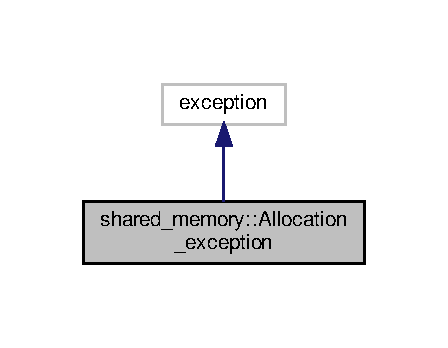
\includegraphics[width=215pt]{classshared__memory_1_1Allocation__exception__inherit__graph}
\end{center}
\end{figure}


Collaboration diagram for shared\+\_\+memory\+:\+:Allocation\+\_\+exception\+:
\nopagebreak
\begin{figure}[H]
\begin{center}
\leavevmode
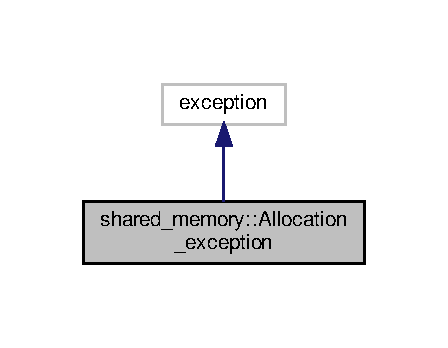
\includegraphics[width=215pt]{classshared__memory_1_1Allocation__exception__coll__graph}
\end{center}
\end{figure}
\subsection*{Public Member Functions}
\begin{DoxyCompactItemize}
\item 
\mbox{\Hypertarget{classshared__memory_1_1Allocation__exception_ac81ff8567ac6c6cec754fefc5fe79d12}\label{classshared__memory_1_1Allocation__exception_ac81ff8567ac6c6cec754fefc5fe79d12}} 
{\bfseries Allocation\+\_\+exception} (const std\+::string \&segment\+\_\+id, const std\+::string \&object\+\_\+id)
\item 
\mbox{\Hypertarget{classshared__memory_1_1Allocation__exception_ace0c58eb354d14879430d339df72c889}\label{classshared__memory_1_1Allocation__exception_ace0c58eb354d14879430d339df72c889}} 
const char $\ast$ {\bfseries what} () const  throw ()
\end{DoxyCompactItemize}
\subsection*{Private Attributes}
\begin{DoxyCompactItemize}
\item 
\mbox{\Hypertarget{classshared__memory_1_1Allocation__exception_a57a0e22bd60d77310cd67371a2294028}\label{classshared__memory_1_1Allocation__exception_a57a0e22bd60d77310cd67371a2294028}} 
std\+::string {\bfseries error\+\_\+message\+\_\+}
\end{DoxyCompactItemize}


The documentation for this class was generated from the following files\+:\begin{DoxyCompactItemize}
\item 
include/shared\+\_\+memory/\hyperlink{exceptions_8h}{exceptions.\+h}\item 
src/\hyperlink{exceptions_8cpp}{exceptions.\+cpp}\end{DoxyCompactItemize}

\hypertarget{classshared__memory_1_1array}{}\section{shared\+\_\+memory\+:\+:array$<$ T, S\+I\+ZE $>$ Class Template Reference}
\label{classshared__memory_1_1array}\index{shared\+\_\+memory\+::array$<$ T, S\+I\+Z\+E $>$@{shared\+\_\+memory\+::array$<$ T, S\+I\+Z\+E $>$}}


Implement a shared array stored on a shared memory segment.  




{\ttfamily \#include $<$array.\+hpp$>$}



Inheritance diagram for shared\+\_\+memory\+:\+:array$<$ T, S\+I\+ZE $>$\+:
\nopagebreak
\begin{figure}[H]
\begin{center}
\leavevmode
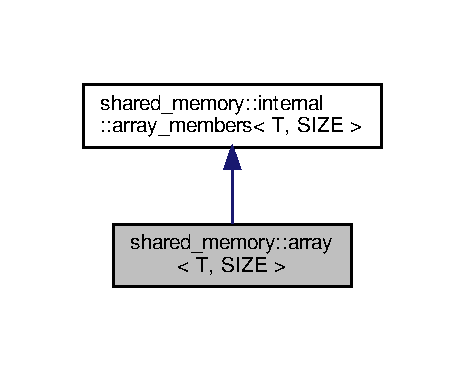
\includegraphics[width=202pt]{classshared__memory_1_1array__inherit__graph}
\end{center}
\end{figure}


Collaboration diagram for shared\+\_\+memory\+:\+:array$<$ T, S\+I\+ZE $>$\+:
\nopagebreak
\begin{figure}[H]
\begin{center}
\leavevmode
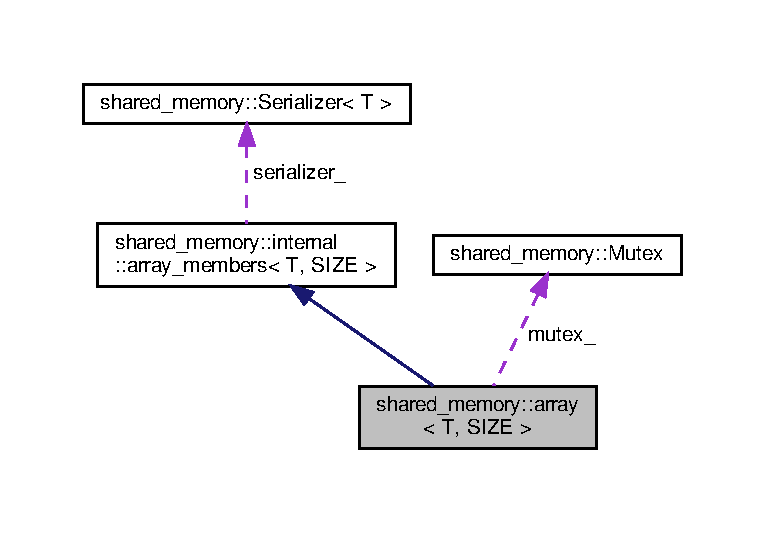
\includegraphics[width=340pt]{classshared__memory_1_1array__coll__graph}
\end{center}
\end{figure}
\subsection*{Public Member Functions}
\begin{DoxyCompactItemize}
\item 
\hyperlink{classshared__memory_1_1array_a95b5abd158cb04ab0644f5aa6df48b2b}{array} (std\+::string segment\+\_\+id, std\+::size\+\_\+t \hyperlink{classshared__memory_1_1array_ad6019f83449e4ea8d1bf4bd0d48c29b0}{size}, bool clear\+\_\+on\+\_\+destruction=true, bool multiprocess\+\_\+safe=true)
\item 
\mbox{\Hypertarget{classshared__memory_1_1array_a45cad350fdb0170c955c8c367a9e910d}\label{classshared__memory_1_1array_a45cad350fdb0170c955c8c367a9e910d}} 
\hyperlink{classshared__memory_1_1array_a45cad350fdb0170c955c8c367a9e910d}{$\sim$array} ()
\begin{DoxyCompactList}\small\item\em wipe the related shared memory segment if clear\+\_\+on\+\_\+destruction is true (true by default) \end{DoxyCompactList}\item 
\mbox{\Hypertarget{classshared__memory_1_1array_acde1531706ba2ab6c05d7639bc0f6f56}\label{classshared__memory_1_1array_acde1531706ba2ab6c05d7639bc0f6f56}} 
\hyperlink{classshared__memory_1_1array_acde1531706ba2ab6c05d7639bc0f6f56}{array} (const \hyperlink{classshared__memory_1_1array}{array}$<$ T, S\+I\+ZE $>$ \&other)
\begin{DoxyCompactList}\small\item\em this array and other array will point to the same memory segment, and will have same values for clear\+\_\+on\+\_\+destruction and multiprocess\+\_\+safe \end{DoxyCompactList}\item 
\hyperlink{classshared__memory_1_1array_af399f2f20d16dadf8381c61ea5ad42fd}{array} (\hyperlink{classshared__memory_1_1array}{array}$<$ T, S\+I\+ZE $>$ \&\&other) noexcept
\begin{DoxyCompactList}\small\item\em This array will point to the share memory segment pointed at by other; and will have same value for multprocess\+\_\+safe and clear\+\_\+on\+\_\+destruction. \end{DoxyCompactList}\item 
\hyperlink{classshared__memory_1_1array}{array}$<$ T, S\+I\+ZE $>$ \& \hyperlink{classshared__memory_1_1array_ad5b4b2841b2785b188a6371cb7f00f1f}{operator=} (\hyperlink{classshared__memory_1_1array}{array}$<$ T, S\+I\+ZE $>$ \&\&other) noexcept
\begin{DoxyCompactList}\small\item\em This array will point to the share memory segment pointed at by other; and will have same value for multprocess\+\_\+safe and clear\+\_\+on\+\_\+destruction. \end{DoxyCompactList}\item 
\mbox{\Hypertarget{classshared__memory_1_1array_ac413bc76d199bb52a0f95faff7222f37}\label{classshared__memory_1_1array_ac413bc76d199bb52a0f95faff7222f37}} 
void \hyperlink{classshared__memory_1_1array_ac413bc76d199bb52a0f95faff7222f37}{set} (uint index, const T \&t)
\begin{DoxyCompactList}\small\item\em set element t at index \end{DoxyCompactList}\item 
\mbox{\Hypertarget{classshared__memory_1_1array_ae581f4ffcf1e543032e0128be5da181d}\label{classshared__memory_1_1array_ae581f4ffcf1e543032e0128be5da181d}} 
void \hyperlink{classshared__memory_1_1array_ae581f4ffcf1e543032e0128be5da181d}{set} (uint index, const T $\ast$t)
\begin{DoxyCompactList}\small\item\em set element t at index \end{DoxyCompactList}\item 
\mbox{\Hypertarget{classshared__memory_1_1array_ae16ed72c9590631e608de8bacf1368ba}\label{classshared__memory_1_1array_ae16ed72c9590631e608de8bacf1368ba}} 
void \hyperlink{classshared__memory_1_1array_ae16ed72c9590631e608de8bacf1368ba}{get} (uint index, T \&t)
\begin{DoxyCompactList}\small\item\em read element at index into t \end{DoxyCompactList}\item 
\mbox{\Hypertarget{classshared__memory_1_1array_ad700d5874d92def07f77f4da7f31f980}\label{classshared__memory_1_1array_ad700d5874d92def07f77f4da7f31f980}} 
void \hyperlink{classshared__memory_1_1array_ad700d5874d92def07f77f4da7f31f980}{get} (uint index, T $\ast$t)
\begin{DoxyCompactList}\small\item\em read element at index into t \end{DoxyCompactList}\item 
\mbox{\Hypertarget{classshared__memory_1_1array_ad6019f83449e4ea8d1bf4bd0d48c29b0}\label{classshared__memory_1_1array_ad6019f83449e4ea8d1bf4bd0d48c29b0}} 
std\+::size\+\_\+t \hyperlink{classshared__memory_1_1array_ad6019f83449e4ea8d1bf4bd0d48c29b0}{size} () const
\begin{DoxyCompactList}\small\item\em max number of elements in the array \end{DoxyCompactList}\item 
\mbox{\Hypertarget{classshared__memory_1_1array_a9e912e143886359921c04fdbba7f6cba}\label{classshared__memory_1_1array_a9e912e143886359921c04fdbba7f6cba}} 
void \hyperlink{classshared__memory_1_1array_a9e912e143886359921c04fdbba7f6cba}{print} ()
\begin{DoxyCompactList}\small\item\em print in terminal info about array\textquotesingle{}s memory usage \end{DoxyCompactList}\item 
\mbox{\Hypertarget{classshared__memory_1_1array_a20e27fb6b9a18e252368c4f6118b3d27}\label{classshared__memory_1_1array_a20e27fb6b9a18e252368c4f6118b3d27}} 
void $\ast$ {\bfseries get\+\_\+raw} ()
\end{DoxyCompactItemize}
\subsection*{Private Member Functions}
\begin{DoxyCompactItemize}
\item 
\mbox{\Hypertarget{classshared__memory_1_1array_a41258d788855ccc8435efb2017bdd068}\label{classshared__memory_1_1array_a41258d788855ccc8435efb2017bdd068}} 
void {\bfseries init} (F\+U\+N\+D\+A\+M\+E\+N\+T\+AL)
\item 
\mbox{\Hypertarget{classshared__memory_1_1array_ad7fa6301507f10efe97ce3ad40187d9f}\label{classshared__memory_1_1array_ad7fa6301507f10efe97ce3ad40187d9f}} 
void {\bfseries set} (uint index, const T \&t, F\+U\+N\+D\+A\+M\+E\+N\+T\+AL)
\item 
\mbox{\Hypertarget{classshared__memory_1_1array_a0a54a689331205da7338f7c5891a6ee5}\label{classshared__memory_1_1array_a0a54a689331205da7338f7c5891a6ee5}} 
void {\bfseries get} (uint index, T \&t, F\+U\+N\+D\+A\+M\+E\+N\+T\+AL)
\item 
\mbox{\Hypertarget{classshared__memory_1_1array_ac0e57adf8e47afae3f8053c20c3e15f2}\label{classshared__memory_1_1array_ac0e57adf8e47afae3f8053c20c3e15f2}} 
void {\bfseries init} (F\+U\+N\+D\+A\+M\+E\+N\+T\+A\+L\+\_\+\+A\+R\+R\+AY)
\item 
\mbox{\Hypertarget{classshared__memory_1_1array_a71bbc60da4a88fd51b3124cdb6cd1ae3}\label{classshared__memory_1_1array_a71bbc60da4a88fd51b3124cdb6cd1ae3}} 
void {\bfseries set} (uint index, const T \&t, F\+U\+N\+D\+A\+M\+E\+N\+T\+A\+L\+\_\+\+A\+R\+R\+AY)
\item 
\mbox{\Hypertarget{classshared__memory_1_1array_af12c8f76fc48b3ec1ff2c2c82d104837}\label{classshared__memory_1_1array_af12c8f76fc48b3ec1ff2c2c82d104837}} 
void {\bfseries get} (uint index, T \&t, F\+U\+N\+D\+A\+M\+E\+N\+T\+A\+L\+\_\+\+A\+R\+R\+AY)
\item 
\mbox{\Hypertarget{classshared__memory_1_1array_a487be484bf27d17f8c7547a57ff995f9}\label{classshared__memory_1_1array_a487be484bf27d17f8c7547a57ff995f9}} 
void {\bfseries init} (S\+E\+R\+I\+A\+L\+I\+Z\+A\+B\+LE)
\item 
\mbox{\Hypertarget{classshared__memory_1_1array_a951c9ca373e942f094910bea57953eb0}\label{classshared__memory_1_1array_a951c9ca373e942f094910bea57953eb0}} 
void {\bfseries set} (uint index, const T \&t, S\+E\+R\+I\+A\+L\+I\+Z\+A\+B\+LE)
\item 
\mbox{\Hypertarget{classshared__memory_1_1array_afb0025021b69b790c152c27ef441cd66}\label{classshared__memory_1_1array_afb0025021b69b790c152c27ef441cd66}} 
void {\bfseries get} (uint index, T \&t, S\+E\+R\+I\+A\+L\+I\+Z\+A\+B\+LE)
\end{DoxyCompactItemize}
\subsection*{Private Attributes}
\begin{DoxyCompactItemize}
\item 
\mbox{\Hypertarget{classshared__memory_1_1array_a43c56477481ae684932b6a03b64d7b67}\label{classshared__memory_1_1array_a43c56477481ae684932b6a03b64d7b67}} 
boost\+::interprocess\+::managed\+\_\+shared\+\_\+memory {\bfseries segment\+\_\+manager\+\_\+}
\item 
\mbox{\Hypertarget{classshared__memory_1_1array_a25a07e97c454f8fb122eb092ab29812c}\label{classshared__memory_1_1array_a25a07e97c454f8fb122eb092ab29812c}} 
std\+::string {\bfseries segment\+\_\+id\+\_\+}
\item 
\mbox{\Hypertarget{classshared__memory_1_1array_a1b47b48a2779e766a80403f47404876a}\label{classshared__memory_1_1array_a1b47b48a2779e766a80403f47404876a}} 
std\+::size\+\_\+t {\bfseries size\+\_\+}
\item 
\mbox{\Hypertarget{classshared__memory_1_1array_afb6fcb395ac52cb9eaaef2882b623d23}\label{classshared__memory_1_1array_afb6fcb395ac52cb9eaaef2882b623d23}} 
bool {\bfseries clear\+\_\+on\+\_\+destruction\+\_\+}
\item 
\mbox{\Hypertarget{classshared__memory_1_1array_a7051346ccb28372b2ea5587714113079}\label{classshared__memory_1_1array_a7051346ccb28372b2ea5587714113079}} 
bool {\bfseries multiprocess\+\_\+safe\+\_\+}
\item 
\mbox{\Hypertarget{classshared__memory_1_1array_afaf6604cf5e2c380f86679e1515e6674}\label{classshared__memory_1_1array_afaf6604cf5e2c380f86679e1515e6674}} 
\hyperlink{classshared__memory_1_1Mutex}{shared\+\_\+memory\+::\+Mutex} {\bfseries mutex\+\_\+}
\end{DoxyCompactItemize}


\subsection{Detailed Description}
\subsubsection*{template$<$typename T, int S\+I\+ZE = 0$>$\newline
class shared\+\_\+memory\+::array$<$ T, S\+I\+Z\+E $>$}

Implement a shared array stored on a shared memory segment. 

Items hosted by the array may be of (1) fundamental type (e.\+g. int, double, char), (2) array of fundamental type (e.\+g. int\mbox{[}10\mbox{]}); or (3) instances of a class implementing a serializable function (see shared\+\_\+memory\+::serializer). 

\subsection{Constructor \& Destructor Documentation}
\mbox{\Hypertarget{classshared__memory_1_1array_a95b5abd158cb04ab0644f5aa6df48b2b}\label{classshared__memory_1_1array_a95b5abd158cb04ab0644f5aa6df48b2b}} 
\index{shared\+\_\+memory\+::array@{shared\+\_\+memory\+::array}!array@{array}}
\index{array@{array}!shared\+\_\+memory\+::array@{shared\+\_\+memory\+::array}}
\subsubsection{\texorpdfstring{array()}{array()}\hspace{0.1cm}{\footnotesize\ttfamily [1/2]}}
{\footnotesize\ttfamily template$<$typename T , int S\+I\+ZE$>$ \\
\hyperlink{classshared__memory_1_1array}{shared\+\_\+memory\+::array}$<$ T, S\+I\+ZE $>$\+::\hyperlink{classshared__memory_1_1array}{array} (\begin{DoxyParamCaption}\item[{std\+::string}]{segment\+\_\+id,  }\item[{std\+::size\+\_\+t}]{size,  }\item[{bool}]{clear\+\_\+on\+\_\+destruction = {\ttfamily true},  }\item[{bool}]{multiprocess\+\_\+safe = {\ttfamily true} }\end{DoxyParamCaption})}


\begin{DoxyParams}{Parameters}
{\em segment\+\_\+id} & should be the same for all array pointing to the same shared memory segment \\
\hline
{\em size} & \+: number of elements to be stored by the array \\
\hline
{\em clear\+\_\+on\+\_\+destruction} & if true, the shared memory segment will be wiped on destruction of the array. Note that any other array pointing to this segment may hang indefinitely as a result. If no arrays pointing to the shared memory segment delete the segment, then users are expected to call \hyperlink{namespaceshared__memory_a0371eb6089f446098adf2f9c106333dc}{shared\+\_\+memory\+::clear\+\_\+array}. Failing to do so may result in new array pointing to a new memory segment of the same id to hang indefinitely at construction. \\
\hline
{\em multiprocess\+\_\+safe} & if false, it is strongly adviced to protect accesses via a \hyperlink{classshared__memory_1_1Mutex}{shared\+\_\+memory\+::\+Mutex} \\
\hline
\end{DoxyParams}
\mbox{\Hypertarget{classshared__memory_1_1array_af399f2f20d16dadf8381c61ea5ad42fd}\label{classshared__memory_1_1array_af399f2f20d16dadf8381c61ea5ad42fd}} 
\index{shared\+\_\+memory\+::array@{shared\+\_\+memory\+::array}!array@{array}}
\index{array@{array}!shared\+\_\+memory\+::array@{shared\+\_\+memory\+::array}}
\subsubsection{\texorpdfstring{array()}{array()}\hspace{0.1cm}{\footnotesize\ttfamily [2/2]}}
{\footnotesize\ttfamily template$<$typename T , int S\+I\+ZE$>$ \\
\hyperlink{classshared__memory_1_1array}{shared\+\_\+memory\+::array}$<$ T, S\+I\+ZE $>$\+::\hyperlink{classshared__memory_1_1array}{array} (\begin{DoxyParamCaption}\item[{\hyperlink{classshared__memory_1_1array}{array}$<$ T, S\+I\+ZE $>$ \&\&}]{other }\end{DoxyParamCaption})\hspace{0.3cm}{\ttfamily [noexcept]}}



This array will point to the share memory segment pointed at by other; and will have same value for multprocess\+\_\+safe and clear\+\_\+on\+\_\+destruction. 

Warning\+: even if other.\+clear\+\_\+on\+\_\+destruction is true, the segment memory will not be wiped on the destruction of other. The duty of deleting the shared memory is passed to the new instance, so to speak 

\subsection{Member Function Documentation}
\mbox{\Hypertarget{classshared__memory_1_1array_ad5b4b2841b2785b188a6371cb7f00f1f}\label{classshared__memory_1_1array_ad5b4b2841b2785b188a6371cb7f00f1f}} 
\index{shared\+\_\+memory\+::array@{shared\+\_\+memory\+::array}!operator=@{operator=}}
\index{operator=@{operator=}!shared\+\_\+memory\+::array@{shared\+\_\+memory\+::array}}
\subsubsection{\texorpdfstring{operator=()}{operator=()}}
{\footnotesize\ttfamily template$<$typename T , int S\+I\+ZE$>$ \\
\hyperlink{classshared__memory_1_1array}{array}$<$ T, S\+I\+ZE $>$ \& array\+::operator= (\begin{DoxyParamCaption}\item[{\hyperlink{classshared__memory_1_1array}{array}$<$ T, S\+I\+ZE $>$ \&\&}]{other }\end{DoxyParamCaption})\hspace{0.3cm}{\ttfamily [noexcept]}}



This array will point to the share memory segment pointed at by other; and will have same value for multprocess\+\_\+safe and clear\+\_\+on\+\_\+destruction. 

Warning\+: even if other.\+clear\+\_\+on\+\_\+destruction is true, the segment memory will not be wiped on the destruction of other. The duty of deleting the shared memory is passed to the new instance, so to speak 

The documentation for this class was generated from the following files\+:\begin{DoxyCompactItemize}
\item 
include/shared\+\_\+memory/array.\+hpp\item 
include/shared\+\_\+memory/array.\+hxx\item 
include/shared\+\_\+memory/array\+\_\+fundamental.\+hxx\item 
include/shared\+\_\+memory/array\+\_\+fundamental\+\_\+array.\+hxx\item 
include/shared\+\_\+memory/array\+\_\+serializable.\+hxx\end{DoxyCompactItemize}

\hypertarget{classshared__memory_1_1ConditionVariable}{}\section{shared\+\_\+memory\+:\+:Condition\+Variable Class Reference}
\label{classshared__memory_1_1ConditionVariable}\index{shared\+\_\+memory\+::\+Condition\+Variable@{shared\+\_\+memory\+::\+Condition\+Variable}}
\subsection*{Public Member Functions}
\begin{DoxyCompactItemize}
\item 
\hyperlink{classshared__memory_1_1ConditionVariable_ae4b6accfbe98b2e23f9e20789cea46f7}{Condition\+Variable} (const std\+::string object\+\_\+id, bool clean\+\_\+memory\+\_\+on\+\_\+destruction)\hypertarget{classshared__memory_1_1ConditionVariable_ae4b6accfbe98b2e23f9e20789cea46f7}{}\label{classshared__memory_1_1ConditionVariable_ae4b6accfbe98b2e23f9e20789cea46f7}

\begin{DoxyCompactList}\small\item\em A condition variable shared over the memory The condition variable is cleaned from the memory on destruction if clean\+\_\+memory\+\_\+on\+\_\+destruction is set to true. \end{DoxyCompactList}\item 
void \hyperlink{classshared__memory_1_1ConditionVariable_abc70cd1401f40e23ca4a6afb33f28bb5}{notify\+\_\+all} ()\hypertarget{classshared__memory_1_1ConditionVariable_abc70cd1401f40e23ca4a6afb33f28bb5}{}\label{classshared__memory_1_1ConditionVariable_abc70cd1401f40e23ca4a6afb33f28bb5}

\begin{DoxyCompactList}\small\item\em notify\+\_\+all is notifying all condition variables with the same mutex \end{DoxyCompactList}\item 
void \hyperlink{classshared__memory_1_1ConditionVariable_a8953b054a1074ab5ef0a9f9b35f58a42}{notify\+\_\+one} ()\hypertarget{classshared__memory_1_1ConditionVariable_a8953b054a1074ab5ef0a9f9b35f58a42}{}\label{classshared__memory_1_1ConditionVariable_a8953b054a1074ab5ef0a9f9b35f58a42}

\begin{DoxyCompactList}\small\item\em notify\+\_\+one notifies one condition variable with the same mutex \end{DoxyCompactList}\item 
bool \hyperlink{classshared__memory_1_1ConditionVariable_af7b1ce584ff9ef9a0925f57cae8e6263}{timed\+\_\+wait} (\hyperlink{classshared__memory_1_1Lock}{Lock} \&lock, long wait\+\_\+nano\+\_\+seconds)
\begin{DoxyCompactList}\small\item\em timed\+\_\+wait wait a notify during a certain certain time and then wake up \end{DoxyCompactList}\item 
void \hyperlink{classshared__memory_1_1ConditionVariable_a8746faccdf81b03dd36c5b405c9ab48d}{wait} (\hyperlink{classshared__memory_1_1Lock}{Lock} \&lock)\hypertarget{classshared__memory_1_1ConditionVariable_a8746faccdf81b03dd36c5b405c9ab48d}{}\label{classshared__memory_1_1ConditionVariable_a8746faccdf81b03dd36c5b405c9ab48d}

\begin{DoxyCompactList}\small\item\em wait waits until another thread notifies this object \end{DoxyCompactList}\end{DoxyCompactItemize}
\subsection*{Static Public Member Functions}
\begin{DoxyCompactItemize}
\item 
static void {\bfseries clean} (const std\+::string object\+\_\+id)\hypertarget{classshared__memory_1_1ConditionVariable_adf6a90466c2bf96cbc08f3ba0246274e}{}\label{classshared__memory_1_1ConditionVariable_adf6a90466c2bf96cbc08f3ba0246274e}

\end{DoxyCompactItemize}
\subsection*{Private Attributes}
\begin{DoxyCompactItemize}
\item 
std\+::string \hyperlink{classshared__memory_1_1ConditionVariable_a496feeef1a7fec080435b68a79bc163d}{condition\+\_\+id\+\_\+}\hypertarget{classshared__memory_1_1ConditionVariable_a496feeef1a7fec080435b68a79bc163d}{}\label{classshared__memory_1_1ConditionVariable_a496feeef1a7fec080435b68a79bc163d}

\begin{DoxyCompactList}\small\item\em condition\+\_\+id\+\_\+ is the condition variable name in the shared memory \end{DoxyCompactList}\item 
bool \hyperlink{classshared__memory_1_1ConditionVariable_a872a5c9305c0dff22ec085b8c8306a0d}{clean\+\_\+memory\+\_\+on\+\_\+destruction\+\_\+}\hypertarget{classshared__memory_1_1ConditionVariable_a872a5c9305c0dff22ec085b8c8306a0d}{}\label{classshared__memory_1_1ConditionVariable_a872a5c9305c0dff22ec085b8c8306a0d}

\begin{DoxyCompactList}\small\item\em if true (the default), clean the shared memory of the hosted mutex and condition. \end{DoxyCompactList}\item 
S\+H\+M\+Condition $\ast$ \hyperlink{classshared__memory_1_1ConditionVariable_a37c6e1a6ca44d30c2a29990e4460803b}{condition\+\_\+variable\+\_\+}\hypertarget{classshared__memory_1_1ConditionVariable_a37c6e1a6ca44d30c2a29990e4460803b}{}\label{classshared__memory_1_1ConditionVariable_a37c6e1a6ca44d30c2a29990e4460803b}

\begin{DoxyCompactList}\small\item\em condition\+\_\+variable\+\_\+ is the boost condition variable that is used \end{DoxyCompactList}\item 
std\+::string \hyperlink{classshared__memory_1_1ConditionVariable_ab8221877ff8551e608d5d4691d3679ae}{mutex\+\_\+id\+\_\+}\hypertarget{classshared__memory_1_1ConditionVariable_ab8221877ff8551e608d5d4691d3679ae}{}\label{classshared__memory_1_1ConditionVariable_ab8221877ff8551e608d5d4691d3679ae}

\begin{DoxyCompactList}\small\item\em mutex\+\_\+id\+\_\+ is the mutex name in the shared memory \end{DoxyCompactList}\end{DoxyCompactItemize}


\subsection{Member Function Documentation}
\index{shared\+\_\+memory\+::\+Condition\+Variable@{shared\+\_\+memory\+::\+Condition\+Variable}!timed\+\_\+wait@{timed\+\_\+wait}}
\index{timed\+\_\+wait@{timed\+\_\+wait}!shared\+\_\+memory\+::\+Condition\+Variable@{shared\+\_\+memory\+::\+Condition\+Variable}}
\subsubsection[{\texorpdfstring{timed\+\_\+wait(\+Lock \&lock, long wait\+\_\+nano\+\_\+seconds)}{timed_wait(Lock &lock, long wait_nano_seconds)}}]{\setlength{\rightskip}{0pt plus 5cm}bool shared\+\_\+memory\+::\+Condition\+Variable\+::timed\+\_\+wait (
\begin{DoxyParamCaption}
\item[{{\bf Lock} \&}]{lock, }
\item[{long}]{wait\+\_\+nano\+\_\+seconds}
\end{DoxyParamCaption}
)}\hypertarget{classshared__memory_1_1ConditionVariable_af7b1ce584ff9ef9a0925f57cae8e6263}{}\label{classshared__memory_1_1ConditionVariable_af7b1ce584ff9ef9a0925f57cae8e6263}


timed\+\_\+wait wait a notify during a certain certain time and then wake up 


\begin{DoxyParams}{Parameters}
{\em wait\+\_\+duration} & in microsecond \\
\hline
\end{DoxyParams}
\begin{DoxyReturn}{Returns}
true\+: the condition variable has been notified, false otherwize 
\end{DoxyReturn}


The documentation for this class was generated from the following files\+:\begin{DoxyCompactItemize}
\item 
include/shared\+\_\+memory/condition\+\_\+variable.\+hpp\item 
src/condition\+\_\+variable.\+cpp\end{DoxyCompactItemize}

\hypertarget{classConfig}{}\section{Config Class Reference}
\label{classConfig}\index{Config@{Config}}
\subsection*{Public Attributes}
\begin{DoxyCompactItemize}
\item 
\mbox{\Hypertarget{classConfig_a090beefb5d61fbeb32fc116b32df30d7}\label{classConfig_a090beefb5d61fbeb32fc116b32df30d7}} 
std\+::vector$<$ int $>$ $\ast$ {\bfseries vector}
\item 
\mbox{\Hypertarget{classConfig_a32ce04a94d39445c2c35dc28e03006ef}\label{classConfig_a32ce04a94d39445c2c35dc28e03006ef}} 
std\+::atomic$<$ bool $>$ $\ast$ {\bfseries running}
\item 
\mbox{\Hypertarget{classConfig_a0ed2027733c661de1fae2dbe70146ab4}\label{classConfig_a0ed2027733c661de1fae2dbe70146ab4}} 
int {\bfseries value}
\item 
\mbox{\Hypertarget{classConfig_a05d75fea9600b821909ef25e947b3167}\label{classConfig_a05d75fea9600b821909ef25e947b3167}} 
std\+::string {\bfseries message}
\item 
\mbox{\Hypertarget{classConfig_aa701cf3ea7f432c2879698446754d320}\label{classConfig_aa701cf3ea7f432c2879698446754d320}} 
std\+::condition\+\_\+variable $\ast$ {\bfseries condition}
\item 
\mbox{\Hypertarget{classConfig_abacf2bdd32d425c995c2ba5b16a896bd}\label{classConfig_abacf2bdd32d425c995c2ba5b16a896bd}} 
std\+::mutex $\ast$ {\bfseries mutex}
\end{DoxyCompactItemize}


The documentation for this class was generated from the following files\+:\begin{DoxyCompactItemize}
\item 
demos/cond\+\_\+var\+\_\+demo.\+cpp\item 
demos/sm\+\_\+cond\+\_\+var\+\_\+demo.\+cpp\end{DoxyCompactItemize}

\hypertarget{classshared__memory_1_1Exchange__manager__consumer}{}\section{shared\+\_\+memory\+:\+:Exchange\+\_\+manager\+\_\+consumer$<$ Serializable, Q\+U\+E\+U\+E\+\_\+\+S\+I\+ZE $>$ Class Template Reference}
\label{classshared__memory_1_1Exchange__manager__consumer}\index{shared\+\_\+memory\+::\+Exchange\+\_\+manager\+\_\+consumer$<$ Serializable, Q\+U\+E\+U\+E\+\_\+\+S\+I\+Z\+E $>$@{shared\+\_\+memory\+::\+Exchange\+\_\+manager\+\_\+consumer$<$ Serializable, Q\+U\+E\+U\+E\+\_\+\+S\+I\+Z\+E $>$}}
\subsection*{Public Member Functions}
\begin{DoxyCompactItemize}
\item 
\hyperlink{classshared__memory_1_1Exchange__manager__consumer_a15b2b91e57fb8c9c60ec354274edf20d}{Exchange\+\_\+manager\+\_\+consumer} (std\+::string segment\+\_\+id, std\+::string object\+\_\+id, bool leading, bool autolock=true)
\begin{DoxyCompactList}\small\item\em An exchange\+\_\+manager\+\_\+consumer reads from the shared memory serialized items produced by an instance of exchange\+\_\+manager\+\_\+producer (which should use the same segment\+\_\+id and object\+\_\+id), possibly running in a separate process. \end{DoxyCompactList}\item 
void \hyperlink{classshared__memory_1_1Exchange__manager__consumer_a1ec59bb41c9de78eb891ea70efe6b8c2}{lock} ()
\begin{DoxyCompactList}\small\item\em lock the mutex required for writting in the shared memory without any collision with any producer. \end{DoxyCompactList}\item 
void \hyperlink{classshared__memory_1_1Exchange__manager__consumer_aaf053702ec1ef8455fc10e70144f6923}{unlock} ()
\begin{DoxyCompactList}\small\item\em unlock the mutex for writting in the shared memory without any collision with any producer. \end{DoxyCompactList}\item 
bool \hyperlink{classshared__memory_1_1Exchange__manager__consumer_ae3e006de034b55e328784d3eacfb1772}{consume} (\hyperlink{classSerializable}{Serializable} \&serializable)
\begin{DoxyCompactList}\small\item\em read from the underlying shared memory a serialized object (set by a producer). \end{DoxyCompactList}\item 
bool \hyperlink{classshared__memory_1_1Exchange__manager__consumer_af1a894d796387d297f848d18d8d55df5}{ready\+\_\+to\+\_\+consume} ()
\begin{DoxyCompactList}\small\item\em returns true if a producer is also running. \end{DoxyCompactList}\item 
bool \hyperlink{classshared__memory_1_1Exchange__manager__consumer_a5e62220c9b50327130cb95683d22b0dc}{purge\+\_\+feedbacks} ()
\begin{DoxyCompactList}\small\item\em When this instance consumes an item, the item id is written in a shared queue for the producer to read (and acquire the feedback the item has been consumed). \end{DoxyCompactList}\item 
int \hyperlink{classshared__memory_1_1Exchange__manager__consumer_ab8651cff750b5cb2ceae97a97b2c7f2d}{nb\+\_\+char\+\_\+read} ()
\begin{DoxyCompactList}\small\item\em returns the number of char that have been read from the exchange queue. \end{DoxyCompactList}\item 
bool {\bfseries is\+\_\+producer\+\_\+queue\+\_\+empty} () const \hypertarget{classshared__memory_1_1Exchange__manager__consumer_ad7d4cd68db87b53a0fe45f08c4adb647}{}\label{classshared__memory_1_1Exchange__manager__consumer_ad7d4cd68db87b53a0fe45f08c4adb647}

\item 
bool {\bfseries is\+\_\+consumer\+\_\+queue\+\_\+empty} () const \hypertarget{classshared__memory_1_1Exchange__manager__consumer_a5d50ce37fd9464f45b973f6e96b81ba3}{}\label{classshared__memory_1_1Exchange__manager__consumer_a5d50ce37fd9464f45b973f6e96b81ba3}

\end{DoxyCompactItemize}
\subsection*{Static Public Member Functions}
\begin{DoxyCompactItemize}
\item 
static void {\bfseries clean\+\_\+mutex} (std\+::string segment\+\_\+id)\hypertarget{classshared__memory_1_1Exchange__manager__consumer_a5aeebd5f2857f73c91fe3212d274909e}{}\label{classshared__memory_1_1Exchange__manager__consumer_a5aeebd5f2857f73c91fe3212d274909e}

\item 
static void {\bfseries clean\+\_\+memory} (std\+::string segment\+\_\+id)\hypertarget{classshared__memory_1_1Exchange__manager__consumer_a828a56d15a0f68edd8e3b395c41b0c0c}{}\label{classshared__memory_1_1Exchange__manager__consumer_a828a56d15a0f68edd8e3b395c41b0c0c}

\end{DoxyCompactItemize}
\subsection*{Private Types}
\begin{DoxyCompactItemize}
\item 
typedef \hyperlink{classshared__memory_1_1internal_1_1Exchange__manager__memory}{Exchange\+\_\+manager\+\_\+memory}$<$ \hyperlink{classSerializable}{Serializable}, Q\+U\+E\+U\+E\+\_\+\+S\+I\+ZE $>$ {\bfseries Memory}\hypertarget{classshared__memory_1_1Exchange__manager__consumer_a1699ba86d1d5b943d428fc1b391abd42}{}\label{classshared__memory_1_1Exchange__manager__consumer_a1699ba86d1d5b943d428fc1b391abd42}

\item 
typedef std\+::shared\+\_\+ptr$<$ \hyperlink{classshared__memory_1_1internal_1_1Exchange__manager__memory}{Memory} $>$ {\bfseries Memory\+\_\+ptr}\hypertarget{classshared__memory_1_1Exchange__manager__consumer_a92ad5c787b53c26d5b3c75712ca539f3}{}\label{classshared__memory_1_1Exchange__manager__consumer_a92ad5c787b53c26d5b3c75712ca539f3}

\end{DoxyCompactItemize}
\subsection*{Private Member Functions}
\begin{DoxyCompactItemize}
\item 
void {\bfseries reset} ()\hypertarget{classshared__memory_1_1Exchange__manager__consumer_a7543d28030c9c3e17b8fd60facc917b2}{}\label{classshared__memory_1_1Exchange__manager__consumer_a7543d28030c9c3e17b8fd60facc917b2}

\end{DoxyCompactItemize}
\subsection*{Private Attributes}
\begin{DoxyCompactItemize}
\item 
Memory\+\_\+ptr {\bfseries memory\+\_\+}\hypertarget{classshared__memory_1_1Exchange__manager__consumer_a65f7ea81649be03ac11b11bc998d5047}{}\label{classshared__memory_1_1Exchange__manager__consumer_a65f7ea81649be03ac11b11bc998d5047}

\item 
bool {\bfseries leading\+\_\+}\hypertarget{classshared__memory_1_1Exchange__manager__consumer_a3d2838c1a3e709dafe1c941f217d8f54}{}\label{classshared__memory_1_1Exchange__manager__consumer_a3d2838c1a3e709dafe1c941f217d8f54}

\item 
bool {\bfseries autolock\+\_\+}\hypertarget{classshared__memory_1_1Exchange__manager__consumer_a6ea7ce15b0da981027f80d3d35825593}{}\label{classshared__memory_1_1Exchange__manager__consumer_a6ea7ce15b0da981027f80d3d35825593}

\item 
std\+::string {\bfseries segment\+\_\+id\+\_\+}\hypertarget{classshared__memory_1_1Exchange__manager__consumer_a830f88a2c6f6d3cf6e0c83353a436742}{}\label{classshared__memory_1_1Exchange__manager__consumer_a830f88a2c6f6d3cf6e0c83353a436742}

\item 
std\+::string {\bfseries object\+\_\+id\+\_\+}\hypertarget{classshared__memory_1_1Exchange__manager__consumer_afbde973522ab55b0a3c49ef6f26fbba5}{}\label{classshared__memory_1_1Exchange__manager__consumer_afbde973522ab55b0a3c49ef6f26fbba5}

\end{DoxyCompactItemize}


\subsection{Constructor \& Destructor Documentation}
\index{shared\+\_\+memory\+::\+Exchange\+\_\+manager\+\_\+consumer@{shared\+\_\+memory\+::\+Exchange\+\_\+manager\+\_\+consumer}!Exchange\+\_\+manager\+\_\+consumer@{Exchange\+\_\+manager\+\_\+consumer}}
\index{Exchange\+\_\+manager\+\_\+consumer@{Exchange\+\_\+manager\+\_\+consumer}!shared\+\_\+memory\+::\+Exchange\+\_\+manager\+\_\+consumer@{shared\+\_\+memory\+::\+Exchange\+\_\+manager\+\_\+consumer}}
\subsubsection[{\texorpdfstring{Exchange\+\_\+manager\+\_\+consumer(std\+::string segment\+\_\+id, std\+::string object\+\_\+id, bool leading, bool autolock=true)}{Exchange_manager_consumer(std::string segment_id, std::string object_id, bool leading, bool autolock=true)}}]{\setlength{\rightskip}{0pt plus 5cm}template$<$class Serializable , int Q\+U\+E\+U\+E\+\_\+\+S\+I\+ZE$>$ Exchange\+\_\+manager\+\_\+consumer\+::\+Exchange\+\_\+manager\+\_\+consumer (
\begin{DoxyParamCaption}
\item[{std\+::string}]{segment\+\_\+id, }
\item[{std\+::string}]{object\+\_\+id, }
\item[{bool}]{leading, }
\item[{bool}]{autolock = {\ttfamily true}}
\end{DoxyParamCaption}
)}\hypertarget{classshared__memory_1_1Exchange__manager__consumer_a15b2b91e57fb8c9c60ec354274edf20d}{}\label{classshared__memory_1_1Exchange__manager__consumer_a15b2b91e57fb8c9c60ec354274edf20d}


An exchange\+\_\+manager\+\_\+consumer reads from the shared memory serialized items produced by an instance of exchange\+\_\+manager\+\_\+producer (which should use the same segment\+\_\+id and object\+\_\+id), possibly running in a separate process. 


\begin{DoxyParams}{Parameters}
{\em segment\+\_\+id} & id of the shared memory segment \\
\hline
{\em object\+\_\+id} & id of the shared memory object prefix \\
\hline
{\em the} & consumer is to be \char`\"{}permanent\char`\"{}, while different producers may provide data. Implies the deletion of the underlying share memory upon destruction. \\
\hline
{\em mutex} & locking mechanism internally managed by the producer. If false, lock has to be \char`\"{}manually\char`\"{} called. This allows for example to set several items in one shot \\
\hline
\end{DoxyParams}


\subsection{Member Function Documentation}
\index{shared\+\_\+memory\+::\+Exchange\+\_\+manager\+\_\+consumer@{shared\+\_\+memory\+::\+Exchange\+\_\+manager\+\_\+consumer}!consume@{consume}}
\index{consume@{consume}!shared\+\_\+memory\+::\+Exchange\+\_\+manager\+\_\+consumer@{shared\+\_\+memory\+::\+Exchange\+\_\+manager\+\_\+consumer}}
\subsubsection[{\texorpdfstring{consume(\+Serializable \&serializable)}{consume(Serializable &serializable)}}]{\setlength{\rightskip}{0pt plus 5cm}template$<$class Serializable , int Q\+U\+E\+U\+E\+\_\+\+S\+I\+ZE$>$ bool Exchange\+\_\+manager\+\_\+consumer\+::consume (
\begin{DoxyParamCaption}
\item[{{\bf Serializable} \&}]{serializable}
\end{DoxyParamCaption}
)}\hypertarget{classshared__memory_1_1Exchange__manager__consumer_ae3e006de034b55e328784d3eacfb1772}{}\label{classshared__memory_1_1Exchange__manager__consumer_ae3e006de034b55e328784d3eacfb1772}


read from the underlying shared memory a serialized object (set by a producer). 

Should be called only if ready\+\_\+to\+\_\+consume returns true. \begin{DoxyReturn}{Returns}
true if an item has been read 
\end{DoxyReturn}
\index{shared\+\_\+memory\+::\+Exchange\+\_\+manager\+\_\+consumer@{shared\+\_\+memory\+::\+Exchange\+\_\+manager\+\_\+consumer}!lock@{lock}}
\index{lock@{lock}!shared\+\_\+memory\+::\+Exchange\+\_\+manager\+\_\+consumer@{shared\+\_\+memory\+::\+Exchange\+\_\+manager\+\_\+consumer}}
\subsubsection[{\texorpdfstring{lock()}{lock()}}]{\setlength{\rightskip}{0pt plus 5cm}template$<$class Serializable , int Q\+U\+E\+U\+E\+\_\+\+S\+I\+ZE$>$ void Exchange\+\_\+manager\+\_\+consumer\+::lock (
\begin{DoxyParamCaption}
{}
\end{DoxyParamCaption}
)}\hypertarget{classshared__memory_1_1Exchange__manager__consumer_a1ec59bb41c9de78eb891ea70efe6b8c2}{}\label{classshared__memory_1_1Exchange__manager__consumer_a1ec59bb41c9de78eb891ea70efe6b8c2}


lock the mutex required for writting in the shared memory without any collision with any producer. 

Should be called before calls to \char`\"{}consume\char`\"{}. Not required if the constructor was called with autolock set to true \index{shared\+\_\+memory\+::\+Exchange\+\_\+manager\+\_\+consumer@{shared\+\_\+memory\+::\+Exchange\+\_\+manager\+\_\+consumer}!nb\+\_\+char\+\_\+read@{nb\+\_\+char\+\_\+read}}
\index{nb\+\_\+char\+\_\+read@{nb\+\_\+char\+\_\+read}!shared\+\_\+memory\+::\+Exchange\+\_\+manager\+\_\+consumer@{shared\+\_\+memory\+::\+Exchange\+\_\+manager\+\_\+consumer}}
\subsubsection[{\texorpdfstring{nb\+\_\+char\+\_\+read()}{nb_char_read()}}]{\setlength{\rightskip}{0pt plus 5cm}template$<$class Serializable , int Q\+U\+E\+U\+E\+\_\+\+S\+I\+ZE$>$ int Exchange\+\_\+manager\+\_\+consumer\+::nb\+\_\+char\+\_\+read (
\begin{DoxyParamCaption}
{}
\end{DoxyParamCaption}
)}\hypertarget{classshared__memory_1_1Exchange__manager__consumer_ab8651cff750b5cb2ceae97a97b2c7f2d}{}\label{classshared__memory_1_1Exchange__manager__consumer_ab8651cff750b5cb2ceae97a97b2c7f2d}


returns the number of char that have been read from the exchange queue. 

For debugging purposes \index{shared\+\_\+memory\+::\+Exchange\+\_\+manager\+\_\+consumer@{shared\+\_\+memory\+::\+Exchange\+\_\+manager\+\_\+consumer}!purge\+\_\+feedbacks@{purge\+\_\+feedbacks}}
\index{purge\+\_\+feedbacks@{purge\+\_\+feedbacks}!shared\+\_\+memory\+::\+Exchange\+\_\+manager\+\_\+consumer@{shared\+\_\+memory\+::\+Exchange\+\_\+manager\+\_\+consumer}}
\subsubsection[{\texorpdfstring{purge\+\_\+feedbacks()}{purge_feedbacks()}}]{\setlength{\rightskip}{0pt plus 5cm}template$<$class Serializable , int Q\+U\+E\+U\+E\+\_\+\+S\+I\+ZE$>$ bool Exchange\+\_\+manager\+\_\+consumer\+::purge\+\_\+feedbacks (
\begin{DoxyParamCaption}
{}
\end{DoxyParamCaption}
)}\hypertarget{classshared__memory_1_1Exchange__manager__consumer_a5e62220c9b50327130cb95683d22b0dc}{}\label{classshared__memory_1_1Exchange__manager__consumer_a5e62220c9b50327130cb95683d22b0dc}


When this instance consumes an item, the item id is written in a shared queue for the producer to read (and acquire the feedback the item has been consumed). 

This shared queue may get full (e.\+g the producer does not read it fast enough), in which case the item id is buffered in this instance. If this instance stops to consume, the buffered item ids will never be written in the shared queue, and the producer will not receive the corresponding feedback. This attempts to write the buffered ids into the queue, and returns true if the buffer is not empty after the call (i.\+e. some feedbacks have not been sent yet), false otherwise. Usage\+: to call before exit until true is returned \index{shared\+\_\+memory\+::\+Exchange\+\_\+manager\+\_\+consumer@{shared\+\_\+memory\+::\+Exchange\+\_\+manager\+\_\+consumer}!ready\+\_\+to\+\_\+consume@{ready\+\_\+to\+\_\+consume}}
\index{ready\+\_\+to\+\_\+consume@{ready\+\_\+to\+\_\+consume}!shared\+\_\+memory\+::\+Exchange\+\_\+manager\+\_\+consumer@{shared\+\_\+memory\+::\+Exchange\+\_\+manager\+\_\+consumer}}
\subsubsection[{\texorpdfstring{ready\+\_\+to\+\_\+consume()}{ready_to_consume()}}]{\setlength{\rightskip}{0pt plus 5cm}template$<$class Serializable , int Q\+U\+E\+U\+E\+\_\+\+S\+I\+ZE$>$ bool Exchange\+\_\+manager\+\_\+consumer\+::ready\+\_\+to\+\_\+consume (
\begin{DoxyParamCaption}
{}
\end{DoxyParamCaption}
)}\hypertarget{classshared__memory_1_1Exchange__manager__consumer_af1a894d796387d297f848d18d8d55df5}{}\label{classshared__memory_1_1Exchange__manager__consumer_af1a894d796387d297f848d18d8d55df5}


returns true if a producer is also running. 

\textquotesingle{}consume\textquotesingle{} should be called only if ready\+\_\+to\+\_\+consume returns true. \index{shared\+\_\+memory\+::\+Exchange\+\_\+manager\+\_\+consumer@{shared\+\_\+memory\+::\+Exchange\+\_\+manager\+\_\+consumer}!unlock@{unlock}}
\index{unlock@{unlock}!shared\+\_\+memory\+::\+Exchange\+\_\+manager\+\_\+consumer@{shared\+\_\+memory\+::\+Exchange\+\_\+manager\+\_\+consumer}}
\subsubsection[{\texorpdfstring{unlock()}{unlock()}}]{\setlength{\rightskip}{0pt plus 5cm}template$<$class Serializable , int Q\+U\+E\+U\+E\+\_\+\+S\+I\+ZE$>$ void Exchange\+\_\+manager\+\_\+consumer\+::unlock (
\begin{DoxyParamCaption}
{}
\end{DoxyParamCaption}
)}\hypertarget{classshared__memory_1_1Exchange__manager__consumer_aaf053702ec1ef8455fc10e70144f6923}{}\label{classshared__memory_1_1Exchange__manager__consumer_aaf053702ec1ef8455fc10e70144f6923}


unlock the mutex for writting in the shared memory without any collision with any producer. 

Not required if the constructor was called with autolock set to true 

The documentation for this class was generated from the following files\+:\begin{DoxyCompactItemize}
\item 
include/shared\+\_\+memory/\hyperlink{exchange__manager__consumer_8hpp}{exchange\+\_\+manager\+\_\+consumer.\+hpp}\item 
include/shared\+\_\+memory/exchange\+\_\+manager\+\_\+consumer.\+hxx\end{DoxyCompactItemize}

\hypertarget{classshared__memory_1_1Exchange__manager__producer}{}\section{shared\+\_\+memory\+:\+:Exchange\+\_\+manager\+\_\+producer$<$ Serializable, Q\+U\+E\+U\+E\+\_\+\+S\+I\+ZE $>$ Class Template Reference}
\label{classshared__memory_1_1Exchange__manager__producer}\index{shared\+\_\+memory\+::\+Exchange\+\_\+manager\+\_\+producer$<$ Serializable, Q\+U\+E\+U\+E\+\_\+\+S\+I\+Z\+E $>$@{shared\+\_\+memory\+::\+Exchange\+\_\+manager\+\_\+producer$<$ Serializable, Q\+U\+E\+U\+E\+\_\+\+S\+I\+Z\+E $>$}}
\subsection*{Public Member Functions}
\begin{DoxyCompactItemize}
\item 
\hyperlink{classshared__memory_1_1Exchange__manager__producer_a3fb01ae44f85b9d8b4a22137f2da90f1}{Exchange\+\_\+manager\+\_\+producer} (std\+::string segment\+\_\+id, std\+::string object\+\_\+id, bool leading, bool autolock=true)
\begin{DoxyCompactList}\small\item\em An exchange\+\_\+manager\+\_\+producer writes in the shared memory serialized items expected to be consumed by an instance of exchange\+\_\+manager\+\_\+consumer (which should use the same segment\+\_\+id and object\+\_\+id), possibly running in a separate process. \end{DoxyCompactList}\item 
bool \hyperlink{classshared__memory_1_1Exchange__manager__producer_a3ef5cfdd196a396edfd6ca502119f839}{ready\+\_\+to\+\_\+produce} ()
\begin{DoxyCompactList}\small\item\em returns true if a consumer is also running. \end{DoxyCompactList}\item 
void \hyperlink{classshared__memory_1_1Exchange__manager__producer_aa39c8b921eeff081111c756bd6d2ca3d}{lock} ()
\begin{DoxyCompactList}\small\item\em lock the mutex required for writting in the shared memory without any collision with any consumer. \end{DoxyCompactList}\item 
void \hyperlink{classshared__memory_1_1Exchange__manager__producer_a9c02040ee5ef8db658f3112ae4b3b969}{unlock} ()
\begin{DoxyCompactList}\small\item\em unlock the mutex for writting in the shared memory without any collision with any consumer. \end{DoxyCompactList}\item 
bool \hyperlink{classshared__memory_1_1Exchange__manager__producer_a0f86798dbbb5bead856c566257bd1b07}{set} (const \hyperlink{classSerializable}{Serializable} \&serializable)
\begin{DoxyCompactList}\small\item\em Set this serializable to be consumed. \end{DoxyCompactList}\item 
void \hyperlink{classshared__memory_1_1Exchange__manager__producer_a733c4c3f794e10590569f94e3f320201}{clear} ()
\begin{DoxyCompactList}\small\item\em removed all elements from the shared queue \end{DoxyCompactList}\item 
\mbox{\Hypertarget{classshared__memory_1_1Exchange__manager__producer_afd8afb25d70407b785484e68d1182c0b}\label{classshared__memory_1_1Exchange__manager__producer_afd8afb25d70407b785484e68d1182c0b}} 
void \hyperlink{classshared__memory_1_1Exchange__manager__producer_afd8afb25d70407b785484e68d1182c0b}{get} (std\+::deque$<$ int $>$ \&get\+\_\+consumed\+\_\+ids)
\begin{DoxyCompactList}\small\item\em write into get\+\_\+consumed\+\_\+ids the ids of serialized items that have been successfully consumed by a consumer \end{DoxyCompactList}\item 
int \hyperlink{classshared__memory_1_1Exchange__manager__producer_ab31e6b87ad4c856736dec15486ed4489}{nb\+\_\+char\+\_\+written} ()
\begin{DoxyCompactList}\small\item\em returns the number of characters that have been serialized and written to the exchange queue. \end{DoxyCompactList}\item 
\mbox{\Hypertarget{classshared__memory_1_1Exchange__manager__producer_a742e8859608d49901d3dafbbe08e4674}\label{classshared__memory_1_1Exchange__manager__producer_a742e8859608d49901d3dafbbe08e4674}} 
void \hyperlink{classshared__memory_1_1Exchange__manager__producer_a742e8859608d49901d3dafbbe08e4674}{reset\+\_\+char\+\_\+count} ()
\begin{DoxyCompactList}\small\item\em reset the count of characters written to the exchange queue to zero \end{DoxyCompactList}\item 
\mbox{\Hypertarget{classshared__memory_1_1Exchange__manager__producer_a4a38c8c14004bc46d254375a63f62096}\label{classshared__memory_1_1Exchange__manager__producer_a4a38c8c14004bc46d254375a63f62096}} 
bool {\bfseries producer\+\_\+queue\+\_\+empty} () const
\item 
\mbox{\Hypertarget{classshared__memory_1_1Exchange__manager__producer_ab8f5eef0601cfdb418eb5d521bfa33d0}\label{classshared__memory_1_1Exchange__manager__producer_ab8f5eef0601cfdb418eb5d521bfa33d0}} 
bool {\bfseries consumer\+\_\+queue\+\_\+empty} () const
\end{DoxyCompactItemize}
\subsection*{Static Public Member Functions}
\begin{DoxyCompactItemize}
\item 
static void \hyperlink{classshared__memory_1_1Exchange__manager__producer_af98fe4321e1fd280b509f5dfd2cf4a5b}{clean\+\_\+mutex} (std\+::string segment\+\_\+id)
\begin{DoxyCompactList}\small\item\em (unlock) and erase the mutex from the shared memory. \end{DoxyCompactList}\item 
static void \hyperlink{classshared__memory_1_1Exchange__manager__producer_a8574f4e075d6f755e567d21d04f24aab}{clean\+\_\+memory} (std\+::string segment\+\_\+id)
\begin{DoxyCompactList}\small\item\em wipe out the corresponding shared memory. \end{DoxyCompactList}\end{DoxyCompactItemize}
\subsection*{Private Types}
\begin{DoxyCompactItemize}
\item 
\mbox{\Hypertarget{classshared__memory_1_1Exchange__manager__producer_a65119cf07c0c10f167c191c9ee913029}\label{classshared__memory_1_1Exchange__manager__producer_a65119cf07c0c10f167c191c9ee913029}} 
typedef \hyperlink{classshared__memory_1_1internal_1_1Exchange__manager__memory}{Exchange\+\_\+manager\+\_\+memory}$<$ \hyperlink{classSerializable}{Serializable}, Q\+U\+E\+U\+E\+\_\+\+S\+I\+ZE $>$ {\bfseries Memory}
\item 
\mbox{\Hypertarget{classshared__memory_1_1Exchange__manager__producer_a7f3d7760ca2d1c01fa88e7a6447a38d7}\label{classshared__memory_1_1Exchange__manager__producer_a7f3d7760ca2d1c01fa88e7a6447a38d7}} 
typedef std\+::shared\+\_\+ptr$<$ \hyperlink{classshared__memory_1_1internal_1_1Exchange__manager__memory}{Memory} $>$ {\bfseries Memory\+\_\+ptr}
\end{DoxyCompactItemize}
\subsection*{Private Member Functions}
\begin{DoxyCompactItemize}
\item 
\mbox{\Hypertarget{classshared__memory_1_1Exchange__manager__producer_a2148cfb2e9a1973089d81237ea5735b9}\label{classshared__memory_1_1Exchange__manager__producer_a2148cfb2e9a1973089d81237ea5735b9}} 
void {\bfseries reset} ()
\end{DoxyCompactItemize}
\subsection*{Private Attributes}
\begin{DoxyCompactItemize}
\item 
\mbox{\Hypertarget{classshared__memory_1_1Exchange__manager__producer_a67f2a2c049dabace06c85a35335d1614}\label{classshared__memory_1_1Exchange__manager__producer_a67f2a2c049dabace06c85a35335d1614}} 
Memory\+\_\+ptr {\bfseries memory\+\_\+}
\item 
\mbox{\Hypertarget{classshared__memory_1_1Exchange__manager__producer_a6d89b939f08bbb9180460a0fab2c877f}\label{classshared__memory_1_1Exchange__manager__producer_a6d89b939f08bbb9180460a0fab2c877f}} 
bool {\bfseries autolock\+\_\+}
\item 
\mbox{\Hypertarget{classshared__memory_1_1Exchange__manager__producer_a4c71d725b7b95e4dd00ecf68232d4ac9}\label{classshared__memory_1_1Exchange__manager__producer_a4c71d725b7b95e4dd00ecf68232d4ac9}} 
bool {\bfseries leading\+\_\+}
\item 
\mbox{\Hypertarget{classshared__memory_1_1Exchange__manager__producer_a96ce58e9619ac28b31b46a81c53c20c2}\label{classshared__memory_1_1Exchange__manager__producer_a96ce58e9619ac28b31b46a81c53c20c2}} 
std\+::string {\bfseries segment\+\_\+id\+\_\+}
\item 
\mbox{\Hypertarget{classshared__memory_1_1Exchange__manager__producer_a57ea2e6076963223331f3b6e78cbbc05}\label{classshared__memory_1_1Exchange__manager__producer_a57ea2e6076963223331f3b6e78cbbc05}} 
std\+::string {\bfseries object\+\_\+id\+\_\+}
\end{DoxyCompactItemize}


\subsection{Constructor \& Destructor Documentation}
\mbox{\Hypertarget{classshared__memory_1_1Exchange__manager__producer_a3fb01ae44f85b9d8b4a22137f2da90f1}\label{classshared__memory_1_1Exchange__manager__producer_a3fb01ae44f85b9d8b4a22137f2da90f1}} 
\index{shared\+\_\+memory\+::\+Exchange\+\_\+manager\+\_\+producer@{shared\+\_\+memory\+::\+Exchange\+\_\+manager\+\_\+producer}!Exchange\+\_\+manager\+\_\+producer@{Exchange\+\_\+manager\+\_\+producer}}
\index{Exchange\+\_\+manager\+\_\+producer@{Exchange\+\_\+manager\+\_\+producer}!shared\+\_\+memory\+::\+Exchange\+\_\+manager\+\_\+producer@{shared\+\_\+memory\+::\+Exchange\+\_\+manager\+\_\+producer}}
\subsubsection{\texorpdfstring{Exchange\+\_\+manager\+\_\+producer()}{Exchange\_manager\_producer()}}
{\footnotesize\ttfamily template$<$class Serializable , int Q\+U\+E\+U\+E\+\_\+\+S\+I\+ZE$>$ \\
Exchange\+\_\+manager\+\_\+producer\+::\+Exchange\+\_\+manager\+\_\+producer (\begin{DoxyParamCaption}\item[{std\+::string}]{segment\+\_\+id,  }\item[{std\+::string}]{object\+\_\+id,  }\item[{bool}]{leading,  }\item[{bool}]{autolock = {\ttfamily true} }\end{DoxyParamCaption})}



An exchange\+\_\+manager\+\_\+producer writes in the shared memory serialized items expected to be consumed by an instance of exchange\+\_\+manager\+\_\+consumer (which should use the same segment\+\_\+id and object\+\_\+id), possibly running in a separate process. 


\begin{DoxyParams}{Parameters}
{\em segment\+\_\+id} & id of the shared memory segment \\
\hline
{\em object\+\_\+id} & id of the shared memory object prefix \\
\hline
{\em autolock} & mutex locking mechanism internally managed by the producer. If false, lock has to be \char`\"{}manually\char`\"{} called. This allows for example to set several items in one shot \\
\hline
{\em clean\+\_\+memory\+\_\+on\+\_\+exit.} & If true, the destructor will clean the underlined shared memory items. \\
\hline
\end{DoxyParams}


\subsection{Member Function Documentation}
\mbox{\Hypertarget{classshared__memory_1_1Exchange__manager__producer_a8574f4e075d6f755e567d21d04f24aab}\label{classshared__memory_1_1Exchange__manager__producer_a8574f4e075d6f755e567d21d04f24aab}} 
\index{shared\+\_\+memory\+::\+Exchange\+\_\+manager\+\_\+producer@{shared\+\_\+memory\+::\+Exchange\+\_\+manager\+\_\+producer}!clean\+\_\+memory@{clean\+\_\+memory}}
\index{clean\+\_\+memory@{clean\+\_\+memory}!shared\+\_\+memory\+::\+Exchange\+\_\+manager\+\_\+producer@{shared\+\_\+memory\+::\+Exchange\+\_\+manager\+\_\+producer}}
\subsubsection{\texorpdfstring{clean\+\_\+memory()}{clean\_memory()}}
{\footnotesize\ttfamily template$<$class Serializable , int Q\+U\+E\+U\+E\+\_\+\+S\+I\+ZE$>$ \\
void Exchange\+\_\+manager\+\_\+producer\+::clean\+\_\+memory (\begin{DoxyParamCaption}\item[{std\+::string}]{segment\+\_\+id }\end{DoxyParamCaption})\hspace{0.3cm}{\ttfamily [static]}}



wipe out the corresponding shared memory. 

To be used if some executable using the exchange manager crashed without calls to destructors. \mbox{\Hypertarget{classshared__memory_1_1Exchange__manager__producer_af98fe4321e1fd280b509f5dfd2cf4a5b}\label{classshared__memory_1_1Exchange__manager__producer_af98fe4321e1fd280b509f5dfd2cf4a5b}} 
\index{shared\+\_\+memory\+::\+Exchange\+\_\+manager\+\_\+producer@{shared\+\_\+memory\+::\+Exchange\+\_\+manager\+\_\+producer}!clean\+\_\+mutex@{clean\+\_\+mutex}}
\index{clean\+\_\+mutex@{clean\+\_\+mutex}!shared\+\_\+memory\+::\+Exchange\+\_\+manager\+\_\+producer@{shared\+\_\+memory\+::\+Exchange\+\_\+manager\+\_\+producer}}
\subsubsection{\texorpdfstring{clean\+\_\+mutex()}{clean\_mutex()}}
{\footnotesize\ttfamily template$<$class Serializable , int Q\+U\+E\+U\+E\+\_\+\+S\+I\+ZE$>$ \\
void Exchange\+\_\+manager\+\_\+producer\+::clean\+\_\+mutex (\begin{DoxyParamCaption}\item[{std\+::string}]{segment\+\_\+id }\end{DoxyParamCaption})\hspace{0.3cm}{\ttfamily [static]}}



(unlock) and erase the mutex from the shared memory. 

To be used if some executable using the exchange manager crashed without calls to destructors. \mbox{\Hypertarget{classshared__memory_1_1Exchange__manager__producer_a733c4c3f794e10590569f94e3f320201}\label{classshared__memory_1_1Exchange__manager__producer_a733c4c3f794e10590569f94e3f320201}} 
\index{shared\+\_\+memory\+::\+Exchange\+\_\+manager\+\_\+producer@{shared\+\_\+memory\+::\+Exchange\+\_\+manager\+\_\+producer}!clear@{clear}}
\index{clear@{clear}!shared\+\_\+memory\+::\+Exchange\+\_\+manager\+\_\+producer@{shared\+\_\+memory\+::\+Exchange\+\_\+manager\+\_\+producer}}
\subsubsection{\texorpdfstring{clear()}{clear()}}
{\footnotesize\ttfamily template$<$class Serializable , int Q\+U\+E\+U\+E\+\_\+\+S\+I\+ZE$>$ \\
void Exchange\+\_\+manager\+\_\+producer\+::clear (\begin{DoxyParamCaption}{ }\end{DoxyParamCaption})}



removed all elements from the shared queue 

\mbox{\Hypertarget{classshared__memory_1_1Exchange__manager__producer_aa39c8b921eeff081111c756bd6d2ca3d}\label{classshared__memory_1_1Exchange__manager__producer_aa39c8b921eeff081111c756bd6d2ca3d}} 
\index{shared\+\_\+memory\+::\+Exchange\+\_\+manager\+\_\+producer@{shared\+\_\+memory\+::\+Exchange\+\_\+manager\+\_\+producer}!lock@{lock}}
\index{lock@{lock}!shared\+\_\+memory\+::\+Exchange\+\_\+manager\+\_\+producer@{shared\+\_\+memory\+::\+Exchange\+\_\+manager\+\_\+producer}}
\subsubsection{\texorpdfstring{lock()}{lock()}}
{\footnotesize\ttfamily template$<$class Serializable , int Q\+U\+E\+U\+E\+\_\+\+S\+I\+ZE$>$ \\
void Exchange\+\_\+manager\+\_\+producer\+::lock (\begin{DoxyParamCaption}{ }\end{DoxyParamCaption})}



lock the mutex required for writting in the shared memory without any collision with any consumer. 

Should be called before calls to \char`\"{}set\char`\"{}. Not required if the constructor was called with autolock set to true \mbox{\Hypertarget{classshared__memory_1_1Exchange__manager__producer_ab31e6b87ad4c856736dec15486ed4489}\label{classshared__memory_1_1Exchange__manager__producer_ab31e6b87ad4c856736dec15486ed4489}} 
\index{shared\+\_\+memory\+::\+Exchange\+\_\+manager\+\_\+producer@{shared\+\_\+memory\+::\+Exchange\+\_\+manager\+\_\+producer}!nb\+\_\+char\+\_\+written@{nb\+\_\+char\+\_\+written}}
\index{nb\+\_\+char\+\_\+written@{nb\+\_\+char\+\_\+written}!shared\+\_\+memory\+::\+Exchange\+\_\+manager\+\_\+producer@{shared\+\_\+memory\+::\+Exchange\+\_\+manager\+\_\+producer}}
\subsubsection{\texorpdfstring{nb\+\_\+char\+\_\+written()}{nb\_char\_written()}}
{\footnotesize\ttfamily template$<$class Serializable , int Q\+U\+E\+U\+E\+\_\+\+S\+I\+ZE$>$ \\
int Exchange\+\_\+manager\+\_\+producer\+::nb\+\_\+char\+\_\+written (\begin{DoxyParamCaption}{ }\end{DoxyParamCaption})}



returns the number of characters that have been serialized and written to the exchange queue. 

For debug purposes. \mbox{\Hypertarget{classshared__memory_1_1Exchange__manager__producer_a3ef5cfdd196a396edfd6ca502119f839}\label{classshared__memory_1_1Exchange__manager__producer_a3ef5cfdd196a396edfd6ca502119f839}} 
\index{shared\+\_\+memory\+::\+Exchange\+\_\+manager\+\_\+producer@{shared\+\_\+memory\+::\+Exchange\+\_\+manager\+\_\+producer}!ready\+\_\+to\+\_\+produce@{ready\+\_\+to\+\_\+produce}}
\index{ready\+\_\+to\+\_\+produce@{ready\+\_\+to\+\_\+produce}!shared\+\_\+memory\+::\+Exchange\+\_\+manager\+\_\+producer@{shared\+\_\+memory\+::\+Exchange\+\_\+manager\+\_\+producer}}
\subsubsection{\texorpdfstring{ready\+\_\+to\+\_\+produce()}{ready\_to\_produce()}}
{\footnotesize\ttfamily template$<$class Serializable , int Q\+U\+E\+U\+E\+\_\+\+S\+I\+ZE$>$ \\
bool Exchange\+\_\+manager\+\_\+producer\+::ready\+\_\+to\+\_\+produce (\begin{DoxyParamCaption}{ }\end{DoxyParamCaption})}



returns true if a consumer is also running. 

\textquotesingle{}set\textquotesingle{} should be called only if ready\+\_\+to\+\_\+produce returns true. \mbox{\Hypertarget{classshared__memory_1_1Exchange__manager__producer_a0f86798dbbb5bead856c566257bd1b07}\label{classshared__memory_1_1Exchange__manager__producer_a0f86798dbbb5bead856c566257bd1b07}} 
\index{shared\+\_\+memory\+::\+Exchange\+\_\+manager\+\_\+producer@{shared\+\_\+memory\+::\+Exchange\+\_\+manager\+\_\+producer}!set@{set}}
\index{set@{set}!shared\+\_\+memory\+::\+Exchange\+\_\+manager\+\_\+producer@{shared\+\_\+memory\+::\+Exchange\+\_\+manager\+\_\+producer}}
\subsubsection{\texorpdfstring{set()}{set()}}
{\footnotesize\ttfamily template$<$class Serializable , int Q\+U\+E\+U\+E\+\_\+\+S\+I\+ZE$>$ \\
bool Exchange\+\_\+manager\+\_\+producer\+::set (\begin{DoxyParamCaption}\item[{const \hyperlink{classSerializable}{Serializable} \&}]{serializable }\end{DoxyParamCaption})}



Set this serializable to be consumed. 

Throws \hyperlink{classshared__memory_1_1Memory__overflow__exception}{shared\+\_\+memory\+::\+Memory\+\_\+overflow\+\_\+exception} if the shared memory is full. Some of the shared memory should get free once items have been consumed by a consumer. This method should be called only if \textquotesingle{}ready\+\_\+to\+\_\+produce\textquotesingle{} returns true; Returns true if all data could be written in the shared memory, false if some data required to be buffered (any following call to set, if any, will perform a new attempt to write remaining buffer to the shared memory) \mbox{\Hypertarget{classshared__memory_1_1Exchange__manager__producer_a9c02040ee5ef8db658f3112ae4b3b969}\label{classshared__memory_1_1Exchange__manager__producer_a9c02040ee5ef8db658f3112ae4b3b969}} 
\index{shared\+\_\+memory\+::\+Exchange\+\_\+manager\+\_\+producer@{shared\+\_\+memory\+::\+Exchange\+\_\+manager\+\_\+producer}!unlock@{unlock}}
\index{unlock@{unlock}!shared\+\_\+memory\+::\+Exchange\+\_\+manager\+\_\+producer@{shared\+\_\+memory\+::\+Exchange\+\_\+manager\+\_\+producer}}
\subsubsection{\texorpdfstring{unlock()}{unlock()}}
{\footnotesize\ttfamily template$<$class Serializable , int Q\+U\+E\+U\+E\+\_\+\+S\+I\+ZE$>$ \\
void Exchange\+\_\+manager\+\_\+producer\+::unlock (\begin{DoxyParamCaption}{ }\end{DoxyParamCaption})}



unlock the mutex for writting in the shared memory without any collision with any consumer. 

Not required if the constructor was called with autolock set to true 

The documentation for this class was generated from the following files\+:\begin{DoxyCompactItemize}
\item 
include/shared\+\_\+memory/\hyperlink{exchange__manager__producer_8hpp}{exchange\+\_\+manager\+\_\+producer.\+hpp}\item 
include/shared\+\_\+memory/exchange\+\_\+manager\+\_\+producer.\+hxx\end{DoxyCompactItemize}

\hypertarget{classshared__memory_1_1Four__int__values}{}\section{shared\+\_\+memory\+:\+:Four\+\_\+int\+\_\+values Class Reference}
\label{classshared__memory_1_1Four__int__values}\index{shared\+\_\+memory\+::\+Four\+\_\+int\+\_\+values@{shared\+\_\+memory\+::\+Four\+\_\+int\+\_\+values}}


Example of an instance that can be serialized.  




{\ttfamily \#include $<$four\+\_\+int\+\_\+values.\+hpp$>$}

\subsection*{Public Member Functions}
\begin{DoxyCompactItemize}
\item 
\mbox{\Hypertarget{classshared__memory_1_1Four__int__values_a28e7fda257450d7650926ae4cec8ea21}\label{classshared__memory_1_1Four__int__values_a28e7fda257450d7650926ae4cec8ea21}} 
{\bfseries Four\+\_\+int\+\_\+values} (int a, int b, int c, int d)
\item 
\mbox{\Hypertarget{classshared__memory_1_1Four__int__values_a90e8357cfc910d419f5d1230118eda22}\label{classshared__memory_1_1Four__int__values_a90e8357cfc910d419f5d1230118eda22}} 
int {\bfseries get\+\_\+id} () const
\item 
\mbox{\Hypertarget{classshared__memory_1_1Four__int__values_aa9904f00f9ae680bab360954e5f3f7a9}\label{classshared__memory_1_1Four__int__values_aa9904f00f9ae680bab360954e5f3f7a9}} 
void {\bfseries set\+\_\+id} (int id)
\item 
\mbox{\Hypertarget{classshared__memory_1_1Four__int__values_ae19116850c04d24ce74dc28bd9cbcf39}\label{classshared__memory_1_1Four__int__values_ae19116850c04d24ce74dc28bd9cbcf39}} 
{\footnotesize template$<$class Archive $>$ }\\void {\bfseries serialize} (Archive \&archive)
\item 
\mbox{\Hypertarget{classshared__memory_1_1Four__int__values_a1ac9c842573728feed000826ced50933}\label{classshared__memory_1_1Four__int__values_a1ac9c842573728feed000826ced50933}} 
bool {\bfseries equal} (const \hyperlink{classshared__memory_1_1Four__int__values}{Four\+\_\+int\+\_\+values} \&other) const
\item 
\mbox{\Hypertarget{classshared__memory_1_1Four__int__values_a64ae65fa773ceca652e78b551466ec9e}\label{classshared__memory_1_1Four__int__values_a64ae65fa773ceca652e78b551466ec9e}} 
bool {\bfseries same} (const \hyperlink{classshared__memory_1_1Four__int__values}{Four\+\_\+int\+\_\+values} \&other) const
\item 
\mbox{\Hypertarget{classshared__memory_1_1Four__int__values_a904e1a3c7724cf9ddb43e62418f87eb0}\label{classshared__memory_1_1Four__int__values_a904e1a3c7724cf9ddb43e62418f87eb0}} 
void {\bfseries print} () const
\end{DoxyCompactItemize}
\subsection*{Static Private Member Functions}
\begin{DoxyCompactItemize}
\item 
\mbox{\Hypertarget{classshared__memory_1_1Four__int__values_a2b34bc8100ec157982d0c6d7a1df14de}\label{classshared__memory_1_1Four__int__values_a2b34bc8100ec157982d0c6d7a1df14de}} 
static int {\bfseries next\+\_\+id} ()
\end{DoxyCompactItemize}
\subsection*{Private Attributes}
\begin{DoxyCompactItemize}
\item 
\mbox{\Hypertarget{classshared__memory_1_1Four__int__values_a692d60e4a7802cad45c215c65632e888}\label{classshared__memory_1_1Four__int__values_a692d60e4a7802cad45c215c65632e888}} 
friend {\bfseries private\+\_\+serialization}
\item 
\mbox{\Hypertarget{classshared__memory_1_1Four__int__values_a253eba8afb24a1679013be704b224ea5}\label{classshared__memory_1_1Four__int__values_a253eba8afb24a1679013be704b224ea5}} 
std\+::vector$<$ int $>$ {\bfseries values\+\_\+}
\item 
\mbox{\Hypertarget{classshared__memory_1_1Four__int__values_a2272823a3c672123c022851611640dd1}\label{classshared__memory_1_1Four__int__values_a2272823a3c672123c022851611640dd1}} 
int {\bfseries id\+\_\+}
\end{DoxyCompactItemize}


\subsection{Detailed Description}
Example of an instance that can be serialized. 

Notice\+: There is a default constructor There is a serialize function It is friend to private\+\_\+serialization 

The documentation for this class was generated from the following files\+:\begin{DoxyCompactItemize}
\item 
include/shared\+\_\+memory/demos/\hyperlink{four__int__values_8hpp}{four\+\_\+int\+\_\+values.\+hpp}\item 
demos/\hyperlink{four__int__values_8cpp}{four\+\_\+int\+\_\+values.\+cpp}\end{DoxyCompactItemize}

\hypertarget{classshared__memory_1_1Item}{}\section{shared\+\_\+memory\+:\+:Item$<$ S\+I\+ZE $>$ Class Template Reference}
\label{classshared__memory_1_1Item}\index{shared\+\_\+memory\+::\+Item$<$ S\+I\+Z\+E $>$@{shared\+\_\+memory\+::\+Item$<$ S\+I\+Z\+E $>$}}
\subsection*{Public Member Functions}
\begin{DoxyCompactItemize}
\item 
{\bfseries Item} (int value)\hypertarget{classshared__memory_1_1Item_a6d7d4864fe09b43ec99356e9c0c62b98}{}\label{classshared__memory_1_1Item_a6d7d4864fe09b43ec99356e9c0c62b98}

\item 
void {\bfseries fill} (int value)\hypertarget{classshared__memory_1_1Item_a765ce924f63067b2df32f4170175611e}{}\label{classshared__memory_1_1Item_a765ce924f63067b2df32f4170175611e}

\item 
void {\bfseries set} (int index, int value)\hypertarget{classshared__memory_1_1Item_a7941efea49faeb757864ae273604fd22}{}\label{classshared__memory_1_1Item_a7941efea49faeb757864ae273604fd22}

\item 
int {\bfseries get} () const \hypertarget{classshared__memory_1_1Item_ac4d6b35bef7d7ddeee7102cd9a245e50}{}\label{classshared__memory_1_1Item_ac4d6b35bef7d7ddeee7102cd9a245e50}

\item 
int {\bfseries get} (int index) const \hypertarget{classshared__memory_1_1Item_abbad388adf21cfb53b84916d10eda23f}{}\label{classshared__memory_1_1Item_abbad388adf21cfb53b84916d10eda23f}

\item 
{\footnotesize template$<$class Archive $>$ }\\void {\bfseries serialize} (Archive \&archive)\hypertarget{classshared__memory_1_1Item_ab48965377a911cf7b625926759b4e0f9}{}\label{classshared__memory_1_1Item_ab48965377a911cf7b625926759b4e0f9}

\item 
void {\bfseries compact\+\_\+print} () const \hypertarget{classshared__memory_1_1Item_ad3ca702e477914370c16f19a77d799b5}{}\label{classshared__memory_1_1Item_ad3ca702e477914370c16f19a77d799b5}

\item 
void {\bfseries print} () const \hypertarget{classshared__memory_1_1Item_a3ff278246a9cb6a7c14f0b0b9370f2a7}{}\label{classshared__memory_1_1Item_a3ff278246a9cb6a7c14f0b0b9370f2a7}

\end{DoxyCompactItemize}
\subsection*{Public Attributes}
\begin{DoxyCompactItemize}
\item 
std\+::array$<$ int, S\+I\+ZE $>$ {\bfseries a\+\_\+}\hypertarget{classshared__memory_1_1Item_a3cb46d7a9776f0512cc8c3689278440b}{}\label{classshared__memory_1_1Item_a3cb46d7a9776f0512cc8c3689278440b}

\item 
int {\bfseries v\+\_\+}\hypertarget{classshared__memory_1_1Item_acd5944f0e62324ef0dc71b91ef9d7054}{}\label{classshared__memory_1_1Item_acd5944f0e62324ef0dc71b91ef9d7054}

\end{DoxyCompactItemize}


The documentation for this class was generated from the following file\+:\begin{DoxyCompactItemize}
\item 
include/shared\+\_\+memory/demos/item.\+hpp\end{DoxyCompactItemize}

\hypertarget{classshared__memory_1_1Lock}{}\section{shared\+\_\+memory\+:\+:Lock Class Reference}
\label{classshared__memory_1_1Lock}\index{shared\+\_\+memory\+::\+Lock@{shared\+\_\+memory\+::\+Lock}}


A scope lock object for locking a shared memory mutex, to use for example with a shared memory condition variable.  




{\ttfamily \#include $<$lock.\+hpp$>$}

\subsection*{Public Member Functions}
\begin{DoxyCompactItemize}
\item 
\mbox{\Hypertarget{classshared__memory_1_1Lock_aacd7b7ee828e6a83bf18497ea7e33d70}\label{classshared__memory_1_1Lock_aacd7b7ee828e6a83bf18497ea7e33d70}} 
\hyperlink{classshared__memory_1_1Lock_aacd7b7ee828e6a83bf18497ea7e33d70}{Lock} (\hyperlink{classshared__memory_1_1Mutex}{Mutex} \&mutex)
\begin{DoxyCompactList}\small\item\em lock the mutex \end{DoxyCompactList}\end{DoxyCompactItemize}
\subsection*{Private Attributes}
\begin{DoxyCompactItemize}
\item 
\mbox{\Hypertarget{classshared__memory_1_1Lock_ab376f06fa4c31a6b2352f307f2bfe007}\label{classshared__memory_1_1Lock_ab376f06fa4c31a6b2352f307f2bfe007}} 
friend {\bfseries Condition\+Variable}
\item 
\mbox{\Hypertarget{classshared__memory_1_1Lock_aa97f73af624861f63cb827b8f8a082f2}\label{classshared__memory_1_1Lock_aa97f73af624861f63cb827b8f8a082f2}} 
S\+H\+M\+Scope\+Lock {\bfseries lock\+\_\+}
\end{DoxyCompactItemize}


\subsection{Detailed Description}
A scope lock object for locking a shared memory mutex, to use for example with a shared memory condition variable. 

The scope is unlocked on destruction. 

The documentation for this class was generated from the following files\+:\begin{DoxyCompactItemize}
\item 
include/shared\+\_\+memory/lock.\+hpp\item 
src/lock.\+cpp\end{DoxyCompactItemize}

\hypertarget{classshared__memory_1_1LockedConditionVariable}{}\section{shared\+\_\+memory\+:\+:Locked\+Condition\+Variable Class Reference}
\label{classshared__memory_1_1LockedConditionVariable}\index{shared\+\_\+memory\+::\+Locked\+Condition\+Variable@{shared\+\_\+memory\+::\+Locked\+Condition\+Variable}}


The \hyperlink{classshared__memory_1_1LockedConditionVariable}{Locked\+Condition\+Variable} class is here as a anonymous layer on top of the boost intersprocess condition variable labrary.  




{\ttfamily \#include $<$locked\+\_\+condition\+\_\+variable.\+hpp$>$}

\subsection*{Public Member Functions}
\begin{DoxyCompactItemize}
\item 
\hyperlink{classshared__memory_1_1LockedConditionVariable_a648057022bbf8a7b5221e1170b1e099c}{Locked\+Condition\+Variable} (const std\+::string object\+\_\+id, bool clean\+\_\+memory\+\_\+on\+\_\+destruction=true)
\begin{DoxyCompactList}\small\item\em A condition variable shared over the memory The condition variable is cleaned from the memory on destruction if clean\+\_\+memory\+\_\+on\+\_\+destruction is set to true. \end{DoxyCompactList}\item 
void \hyperlink{classshared__memory_1_1LockedConditionVariable_a31633f2243b988dc0a8bd3d4637dc216}{notify\+\_\+all} ()\hypertarget{classshared__memory_1_1LockedConditionVariable_a31633f2243b988dc0a8bd3d4637dc216}{}\label{classshared__memory_1_1LockedConditionVariable_a31633f2243b988dc0a8bd3d4637dc216}

\begin{DoxyCompactList}\small\item\em notify\+\_\+all is notifying all condition variables with the same mutex \end{DoxyCompactList}\item 
void \hyperlink{classshared__memory_1_1LockedConditionVariable_a532a1332fe184e668a49fa002db5be08}{notify\+\_\+one} ()\hypertarget{classshared__memory_1_1LockedConditionVariable_a532a1332fe184e668a49fa002db5be08}{}\label{classshared__memory_1_1LockedConditionVariable_a532a1332fe184e668a49fa002db5be08}

\begin{DoxyCompactList}\small\item\em notify\+\_\+one notifies one condition variable with the same mutex \end{DoxyCompactList}\item 
void \hyperlink{classshared__memory_1_1LockedConditionVariable_a9eb84ab5d570a0c5a81f6eaeb4c4dd50}{wait} ()\hypertarget{classshared__memory_1_1LockedConditionVariable_a9eb84ab5d570a0c5a81f6eaeb4c4dd50}{}\label{classshared__memory_1_1LockedConditionVariable_a9eb84ab5d570a0c5a81f6eaeb4c4dd50}

\begin{DoxyCompactList}\small\item\em wait waits until another thread notifies this object \end{DoxyCompactList}\item 
bool \hyperlink{classshared__memory_1_1LockedConditionVariable_a0d4ab218fc51fcce34146f2adca408d7}{timed\+\_\+wait} (long wait\+\_\+nano\+\_\+seconds)
\begin{DoxyCompactList}\small\item\em timed\+\_\+wait wait a notify during a certain certain time and then wake up \end{DoxyCompactList}\item 
bool \hyperlink{classshared__memory_1_1LockedConditionVariable_a86b42b23b94593bca5b12b9d792d1275}{try\+\_\+lock} ()
\begin{DoxyCompactList}\small\item\em try\+\_\+lock Tries to acquire the lock without waiting. \end{DoxyCompactList}\item 
void \hyperlink{classshared__memory_1_1LockedConditionVariable_a5d28bb5942fc5bc4886014d6b9b26885}{unlock} ()
\begin{DoxyCompactList}\small\item\em unlock Unlocks the lock. \end{DoxyCompactList}\item 
bool {\bfseries owns} ()\hypertarget{classshared__memory_1_1LockedConditionVariable_a30e3825249516387276801f8d2e68a8e}{}\label{classshared__memory_1_1LockedConditionVariable_a30e3825249516387276801f8d2e68a8e}

\item 
void \hyperlink{classshared__memory_1_1LockedConditionVariable_a1eef63f7e3e898c3734923c987383ffe}{lock\+\_\+scope} ()
\begin{DoxyCompactList}\small\item\em lock\+\_\+scope this function is used to lock the part of the code that needs protection. \end{DoxyCompactList}\item 
void \hyperlink{classshared__memory_1_1LockedConditionVariable_adf3a50665011b3b92b80369bbbc6d4a4}{unlock\+\_\+scope} ()\hypertarget{classshared__memory_1_1LockedConditionVariable_adf3a50665011b3b92b80369bbbc6d4a4}{}\label{classshared__memory_1_1LockedConditionVariable_adf3a50665011b3b92b80369bbbc6d4a4}

\begin{DoxyCompactList}\small\item\em unlock\+\_\+scope this function unlock the mutex so remove the protection of the code \end{DoxyCompactList}\end{DoxyCompactItemize}
\subsection*{Static Public Member Functions}
\begin{DoxyCompactItemize}
\item 
static void \hyperlink{classshared__memory_1_1LockedConditionVariable_aa3bca5020f84c8e0a90a2dad3e6521e5}{clean} (const std\+::string segment\+\_\+id)
\begin{DoxyCompactList}\small\item\em \hyperlink{classshared__memory_1_1LockedConditionVariable}{Locked\+Condition\+Variable} clean their shared memory on destruction. \end{DoxyCompactList}\end{DoxyCompactItemize}
\subsection*{Public Attributes}
\begin{DoxyCompactItemize}
\item 
S\+H\+M\+Mutex \hyperlink{classshared__memory_1_1LockedConditionVariable_a757abc2190906a0773667b42be6e4e66}{mutex\+\_\+}\hypertarget{classshared__memory_1_1LockedConditionVariable_a757abc2190906a0773667b42be6e4e66}{}\label{classshared__memory_1_1LockedConditionVariable_a757abc2190906a0773667b42be6e4e66}

\begin{DoxyCompactList}\small\item\em mutex\+\_\+ is the mutex associated to the condition variable \end{DoxyCompactList}\item 
S\+H\+M\+Condition $\ast$ \hyperlink{classshared__memory_1_1LockedConditionVariable_a8bc7fb73332304b406335e38ba4cdd1b}{condition\+\_\+variable\+\_\+}\hypertarget{classshared__memory_1_1LockedConditionVariable_a8bc7fb73332304b406335e38ba4cdd1b}{}\label{classshared__memory_1_1LockedConditionVariable_a8bc7fb73332304b406335e38ba4cdd1b}

\begin{DoxyCompactList}\small\item\em condition\+\_\+variable\+\_\+ is the boost condition variable that is used \end{DoxyCompactList}\item 
std\+::unique\+\_\+ptr$<$ S\+H\+M\+Scope\+Lock $>$ \hyperlink{classshared__memory_1_1LockedConditionVariable_a5509b431f2d459d92bfcc1b2d60651d1}{lock\+\_\+}\hypertarget{classshared__memory_1_1LockedConditionVariable_a5509b431f2d459d92bfcc1b2d60651d1}{}\label{classshared__memory_1_1LockedConditionVariable_a5509b431f2d459d92bfcc1b2d60651d1}

\begin{DoxyCompactList}\small\item\em lock\+\_\+ is a object that protects the codes with a mutex, see the boost documentation about \char`\"{}boost\+::interprocess\+::scoped\+\_\+lock\char`\"{} \end{DoxyCompactList}\item 
bool \hyperlink{classshared__memory_1_1LockedConditionVariable_abe0963bc5746d19350e816ad42ff47b1}{clean\+\_\+memory\+\_\+on\+\_\+destruction\+\_\+}\hypertarget{classshared__memory_1_1LockedConditionVariable_abe0963bc5746d19350e816ad42ff47b1}{}\label{classshared__memory_1_1LockedConditionVariable_abe0963bc5746d19350e816ad42ff47b1}

\begin{DoxyCompactList}\small\item\em if true (the default), clean the shared memory of the hosted mutex and condition. \end{DoxyCompactList}\end{DoxyCompactItemize}
\subsection*{Private Attributes}
\begin{DoxyCompactItemize}
\item 
std\+::string \hyperlink{classshared__memory_1_1LockedConditionVariable_a07d7d718e33cc2e833cf9bb22fe8fada}{mutex\+\_\+id\+\_\+}\hypertarget{classshared__memory_1_1LockedConditionVariable_a07d7d718e33cc2e833cf9bb22fe8fada}{}\label{classshared__memory_1_1LockedConditionVariable_a07d7d718e33cc2e833cf9bb22fe8fada}

\begin{DoxyCompactList}\small\item\em mutex\+\_\+id\+\_\+ is the mutex name in the shared memory \end{DoxyCompactList}\item 
std\+::string \hyperlink{classshared__memory_1_1LockedConditionVariable_a7cf01915f9d1a8795f4e69345cd1e1e4}{condition\+\_\+id\+\_\+}\hypertarget{classshared__memory_1_1LockedConditionVariable_a7cf01915f9d1a8795f4e69345cd1e1e4}{}\label{classshared__memory_1_1LockedConditionVariable_a7cf01915f9d1a8795f4e69345cd1e1e4}

\begin{DoxyCompactList}\small\item\em condition\+\_\+id\+\_\+ is the condition variable name in the shared memory \end{DoxyCompactList}\item 
boost\+::interprocess\+::managed\+\_\+shared\+\_\+memory \hyperlink{classshared__memory_1_1LockedConditionVariable_ae6a197846be3bd4ccf4899754778f16b}{segment\+\_\+manager\+\_\+}\hypertarget{classshared__memory_1_1LockedConditionVariable_ae6a197846be3bd4ccf4899754778f16b}{}\label{classshared__memory_1_1LockedConditionVariable_ae6a197846be3bd4ccf4899754778f16b}

\begin{DoxyCompactList}\small\item\em shm\+\_\+segment is the boost object that manages the shared memory segment \end{DoxyCompactList}\end{DoxyCompactItemize}


\subsection{Detailed Description}
The \hyperlink{classshared__memory_1_1LockedConditionVariable}{Locked\+Condition\+Variable} class is here as a anonymous layer on top of the boost intersprocess condition variable labrary. 

It creates a condition variable in a shared memory automatically. 

\subsection{Constructor \& Destructor Documentation}
\index{shared\+\_\+memory\+::\+Locked\+Condition\+Variable@{shared\+\_\+memory\+::\+Locked\+Condition\+Variable}!Locked\+Condition\+Variable@{Locked\+Condition\+Variable}}
\index{Locked\+Condition\+Variable@{Locked\+Condition\+Variable}!shared\+\_\+memory\+::\+Locked\+Condition\+Variable@{shared\+\_\+memory\+::\+Locked\+Condition\+Variable}}
\subsubsection[{\texorpdfstring{Locked\+Condition\+Variable(const std\+::string object\+\_\+id, bool clean\+\_\+memory\+\_\+on\+\_\+destruction=true)}{LockedConditionVariable(const std::string object_id, bool clean_memory_on_destruction=true)}}]{\setlength{\rightskip}{0pt plus 5cm}shared\+\_\+memory\+::\+Locked\+Condition\+Variable\+::\+Locked\+Condition\+Variable (
\begin{DoxyParamCaption}
\item[{const std\+::string}]{object\+\_\+id, }
\item[{bool}]{clean\+\_\+memory\+\_\+on\+\_\+destruction = {\ttfamily true}}
\end{DoxyParamCaption}
)}\hypertarget{classshared__memory_1_1LockedConditionVariable_a648057022bbf8a7b5221e1170b1e099c}{}\label{classshared__memory_1_1LockedConditionVariable_a648057022bbf8a7b5221e1170b1e099c}


A condition variable shared over the memory The condition variable is cleaned from the memory on destruction if clean\+\_\+memory\+\_\+on\+\_\+destruction is set to true. 

Contrary to \hyperlink{classshared__memory_1_1ConditionVariable}{shared\+\_\+memory\+::\+Condition\+Variable}, instances of this class manages their mutex and lock internally, with the consequence the mutex can be locked and unlocked exclusively through other instances of \hyperlink{classshared__memory_1_1LockedConditionVariable}{Locked\+Condition\+Variable}. 

\subsection{Member Function Documentation}
\index{shared\+\_\+memory\+::\+Locked\+Condition\+Variable@{shared\+\_\+memory\+::\+Locked\+Condition\+Variable}!clean@{clean}}
\index{clean@{clean}!shared\+\_\+memory\+::\+Locked\+Condition\+Variable@{shared\+\_\+memory\+::\+Locked\+Condition\+Variable}}
\subsubsection[{\texorpdfstring{clean(const std\+::string segment\+\_\+id)}{clean(const std::string segment_id)}}]{\setlength{\rightskip}{0pt plus 5cm}void shared\+\_\+memory\+::\+Locked\+Condition\+Variable\+::clean (
\begin{DoxyParamCaption}
\item[{const std\+::string}]{segment\+\_\+id}
\end{DoxyParamCaption}
)\hspace{0.3cm}{\ttfamily [static]}}\hypertarget{classshared__memory_1_1LockedConditionVariable_aa3bca5020f84c8e0a90a2dad3e6521e5}{}\label{classshared__memory_1_1LockedConditionVariable_aa3bca5020f84c8e0a90a2dad3e6521e5}


\hyperlink{classshared__memory_1_1LockedConditionVariable}{Locked\+Condition\+Variable} clean their shared memory on destruction. 

But the destructor may have failed to be called if for some reason the program crashed. \index{shared\+\_\+memory\+::\+Locked\+Condition\+Variable@{shared\+\_\+memory\+::\+Locked\+Condition\+Variable}!lock\+\_\+scope@{lock\+\_\+scope}}
\index{lock\+\_\+scope@{lock\+\_\+scope}!shared\+\_\+memory\+::\+Locked\+Condition\+Variable@{shared\+\_\+memory\+::\+Locked\+Condition\+Variable}}
\subsubsection[{\texorpdfstring{lock\+\_\+scope()}{lock_scope()}}]{\setlength{\rightskip}{0pt plus 5cm}void shared\+\_\+memory\+::\+Locked\+Condition\+Variable\+::lock\+\_\+scope (
\begin{DoxyParamCaption}
{}
\end{DoxyParamCaption}
)}\hypertarget{classshared__memory_1_1LockedConditionVariable_a1eef63f7e3e898c3734923c987383ffe}{}\label{classshared__memory_1_1LockedConditionVariable_a1eef63f7e3e898c3734923c987383ffe}


lock\+\_\+scope this function is used to lock the part of the code that needs protection. 

It locks the mutex until unlock\+\_\+scope is used \index{shared\+\_\+memory\+::\+Locked\+Condition\+Variable@{shared\+\_\+memory\+::\+Locked\+Condition\+Variable}!timed\+\_\+wait@{timed\+\_\+wait}}
\index{timed\+\_\+wait@{timed\+\_\+wait}!shared\+\_\+memory\+::\+Locked\+Condition\+Variable@{shared\+\_\+memory\+::\+Locked\+Condition\+Variable}}
\subsubsection[{\texorpdfstring{timed\+\_\+wait(long wait\+\_\+nano\+\_\+seconds)}{timed_wait(long wait_nano_seconds)}}]{\setlength{\rightskip}{0pt plus 5cm}bool shared\+\_\+memory\+::\+Locked\+Condition\+Variable\+::timed\+\_\+wait (
\begin{DoxyParamCaption}
\item[{long}]{wait\+\_\+nano\+\_\+seconds}
\end{DoxyParamCaption}
)}\hypertarget{classshared__memory_1_1LockedConditionVariable_a0d4ab218fc51fcce34146f2adca408d7}{}\label{classshared__memory_1_1LockedConditionVariable_a0d4ab218fc51fcce34146f2adca408d7}


timed\+\_\+wait wait a notify during a certain certain time and then wake up 


\begin{DoxyParams}{Parameters}
{\em wait\+\_\+duration} & in microsecond \\
\hline
\end{DoxyParams}
\begin{DoxyReturn}{Returns}
true\+: the condition variable has been notified, false otherwize 
\end{DoxyReturn}
\index{shared\+\_\+memory\+::\+Locked\+Condition\+Variable@{shared\+\_\+memory\+::\+Locked\+Condition\+Variable}!try\+\_\+lock@{try\+\_\+lock}}
\index{try\+\_\+lock@{try\+\_\+lock}!shared\+\_\+memory\+::\+Locked\+Condition\+Variable@{shared\+\_\+memory\+::\+Locked\+Condition\+Variable}}
\subsubsection[{\texorpdfstring{try\+\_\+lock()}{try_lock()}}]{\setlength{\rightskip}{0pt plus 5cm}bool shared\+\_\+memory\+::\+Locked\+Condition\+Variable\+::try\+\_\+lock (
\begin{DoxyParamCaption}
{}
\end{DoxyParamCaption}
)}\hypertarget{classshared__memory_1_1LockedConditionVariable_a86b42b23b94593bca5b12b9d792d1275}{}\label{classshared__memory_1_1LockedConditionVariable_a86b42b23b94593bca5b12b9d792d1275}


try\+\_\+lock Tries to acquire the lock without waiting. 

\begin{DoxyReturn}{Returns}
true if manages to acquire the lock, false otherwise. 
\end{DoxyReturn}

\begin{DoxyExceptions}{Exceptions}
{\em } & \\
\hline
\end{DoxyExceptions}
\index{shared\+\_\+memory\+::\+Locked\+Condition\+Variable@{shared\+\_\+memory\+::\+Locked\+Condition\+Variable}!unlock@{unlock}}
\index{unlock@{unlock}!shared\+\_\+memory\+::\+Locked\+Condition\+Variable@{shared\+\_\+memory\+::\+Locked\+Condition\+Variable}}
\subsubsection[{\texorpdfstring{unlock()}{unlock()}}]{\setlength{\rightskip}{0pt plus 5cm}void shared\+\_\+memory\+::\+Locked\+Condition\+Variable\+::unlock (
\begin{DoxyParamCaption}
{}
\end{DoxyParamCaption}
)}\hypertarget{classshared__memory_1_1LockedConditionVariable_a5d28bb5942fc5bc4886014d6b9b26885}{}\label{classshared__memory_1_1LockedConditionVariable_a5d28bb5942fc5bc4886014d6b9b26885}


unlock Unlocks the lock. 


\begin{DoxyExceptions}{Exceptions}
{\em } & \\
\hline
\end{DoxyExceptions}


The documentation for this class was generated from the following files\+:\begin{DoxyCompactItemize}
\item 
include/shared\+\_\+memory/locked\+\_\+condition\+\_\+variable.\+hpp\item 
src/locked\+\_\+condition\+\_\+variable.\+cpp\end{DoxyCompactItemize}

\hypertarget{structMeasureTime}{}\section{Measure\+Time Struct Reference}
\label{structMeasureTime}\index{Measure\+Time@{Measure\+Time}}
\subsection*{Public Member Functions}
\begin{DoxyCompactItemize}
\item 
void {\bfseries start} ()\hypertarget{structMeasureTime_a6ca73f3044c7d89271904c43e2f9dc2c}{}\label{structMeasureTime_a6ca73f3044c7d89271904c43e2f9dc2c}

\item 
void {\bfseries update} ()\hypertarget{structMeasureTime_a1714eb45e5ed00a6c90ed36f5d88166a}{}\label{structMeasureTime_a1714eb45e5ed00a6c90ed36f5d88166a}

\end{DoxyCompactItemize}
\subsection*{Public Attributes}
\begin{DoxyCompactItemize}
\item 
Time\+Type {\bfseries tic\+\_\+}\hypertarget{structMeasureTime_a1bfc128b5d3e0f76e99f809acc985ea2}{}\label{structMeasureTime_a1bfc128b5d3e0f76e99f809acc985ea2}

\item 
Time\+Type {\bfseries prev\+\_\+tic\+\_\+}\hypertarget{structMeasureTime_a7a84fdaf6c46c7de792aca6a13ad6382}{}\label{structMeasureTime_a7a84fdaf6c46c7de792aca6a13ad6382}

\item 
double {\bfseries frequency\+\_\+}\hypertarget{structMeasureTime_a5b76f0c97263601aa07d05272e264735}{}\label{structMeasureTime_a5b76f0c97263601aa07d05272e264735}

\item 
double {\bfseries period\+\_\+}\hypertarget{structMeasureTime_a82f4db9bb7b6ae41a8a02d3c25a9a0ff}{}\label{structMeasureTime_a82f4db9bb7b6ae41a8a02d3c25a9a0ff}

\end{DoxyCompactItemize}
\subsection*{Friends}
\begin{DoxyCompactItemize}
\item 
std\+::ostream \& {\bfseries operator$<$$<$} (std\+::ostream \&os, const \hyperlink{structMeasureTime}{Measure\+Time} \&dt)\hypertarget{structMeasureTime_a610d259dacbe716701935d50ecba7780}{}\label{structMeasureTime_a610d259dacbe716701935d50ecba7780}

\end{DoxyCompactItemize}


The documentation for this struct was generated from the following file\+:\begin{DoxyCompactItemize}
\item 
include/shared\+\_\+memory/benchmarks/\hyperlink{benchmark__common_8hh}{benchmark\+\_\+common.\+hh}\end{DoxyCompactItemize}

\hypertarget{classshared__memory_1_1Memory__overflow__exception}{}\section{shared\+\_\+memory\+:\+:Memory\+\_\+overflow\+\_\+exception Class Reference}
\label{classshared__memory_1_1Memory__overflow__exception}\index{shared\+\_\+memory\+::\+Memory\+\_\+overflow\+\_\+exception@{shared\+\_\+memory\+::\+Memory\+\_\+overflow\+\_\+exception}}


Inheritance diagram for shared\+\_\+memory\+:\+:Memory\+\_\+overflow\+\_\+exception\+:
\nopagebreak
\begin{figure}[H]
\begin{center}
\leavevmode
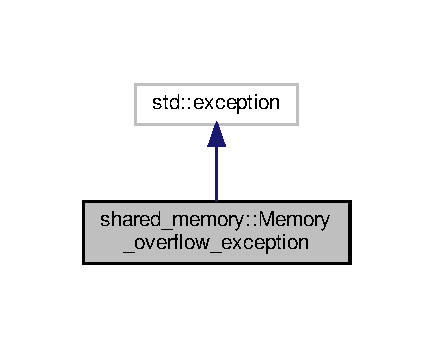
\includegraphics[width=208pt]{classshared__memory_1_1Memory__overflow__exception__inherit__graph}
\end{center}
\end{figure}


Collaboration diagram for shared\+\_\+memory\+:\+:Memory\+\_\+overflow\+\_\+exception\+:
\nopagebreak
\begin{figure}[H]
\begin{center}
\leavevmode
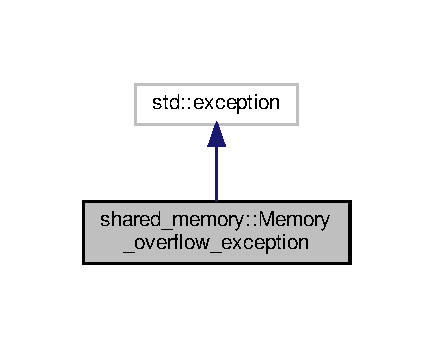
\includegraphics[width=208pt]{classshared__memory_1_1Memory__overflow__exception__coll__graph}
\end{center}
\end{figure}
\subsection*{Public Member Functions}
\begin{DoxyCompactItemize}
\item 
{\bfseries Memory\+\_\+overflow\+\_\+exception} (const std\+::string error\+\_\+message)\hypertarget{classshared__memory_1_1Memory__overflow__exception_aed67eae5c2822873debe5eb8a7427c0b}{}\label{classshared__memory_1_1Memory__overflow__exception_aed67eae5c2822873debe5eb8a7427c0b}

\item 
const char $\ast$ {\bfseries what} () const   throw ()\hypertarget{classshared__memory_1_1Memory__overflow__exception_a378f3443041b2f5fd52e2fd0231d5aea}{}\label{classshared__memory_1_1Memory__overflow__exception_a378f3443041b2f5fd52e2fd0231d5aea}

\end{DoxyCompactItemize}
\subsection*{Private Attributes}
\begin{DoxyCompactItemize}
\item 
std\+::string {\bfseries error\+\_\+message\+\_\+}\hypertarget{classshared__memory_1_1Memory__overflow__exception_ad63afdde056259c8fb0bd3212031783d}{}\label{classshared__memory_1_1Memory__overflow__exception_ad63afdde056259c8fb0bd3212031783d}

\end{DoxyCompactItemize}


The documentation for this class was generated from the following files\+:\begin{DoxyCompactItemize}
\item 
include/shared\+\_\+memory/\hyperlink{exceptions_8h}{exceptions.\+h}\item 
src/\hyperlink{exceptions_8cpp}{exceptions.\+cpp}\end{DoxyCompactItemize}

\hypertarget{classshared__memory_1_1Mutex}{}\section{shared\+\_\+memory\+:\+:Mutex Class Reference}
\label{classshared__memory_1_1Mutex}\index{shared\+\_\+memory\+::\+Mutex@{shared\+\_\+memory\+::\+Mutex}}
\subsection*{Public Member Functions}
\begin{DoxyCompactItemize}
\item 
\mbox{\Hypertarget{classshared__memory_1_1Mutex_a8f1b1cffa2f3bdfb8cd74cf61b0df650}\label{classshared__memory_1_1Mutex_a8f1b1cffa2f3bdfb8cd74cf61b0df650}} 
\hyperlink{classshared__memory_1_1Mutex_a8f1b1cffa2f3bdfb8cd74cf61b0df650}{Mutex} (std\+::string mutex\+\_\+id, bool clean\+\_\+memory\+\_\+on\+\_\+destruction=true)
\begin{DoxyCompactList}\small\item\em A \hyperlink{classshared__memory_1_1Mutex}{Mutex} accessible to several processes via the shared memory The mutex is cleaned from the shared memory on destruction if clean\+\_\+memory\+\_\+on\+\_\+destruction is true (the default) \end{DoxyCompactList}\item 
\mbox{\Hypertarget{classshared__memory_1_1Mutex_a6b6ca2e15d379a5e3a8d68d15c04469f}\label{classshared__memory_1_1Mutex_a6b6ca2e15d379a5e3a8d68d15c04469f}} 
void \hyperlink{classshared__memory_1_1Mutex_a6b6ca2e15d379a5e3a8d68d15c04469f}{lock} ()
\begin{DoxyCompactList}\small\item\em lock the mutex \end{DoxyCompactList}\item 
\mbox{\Hypertarget{classshared__memory_1_1Mutex_a06b9e214880af7ab9703bd78601ac0c6}\label{classshared__memory_1_1Mutex_a06b9e214880af7ab9703bd78601ac0c6}} 
void \hyperlink{classshared__memory_1_1Mutex_a06b9e214880af7ab9703bd78601ac0c6}{unlock} ()
\begin{DoxyCompactList}\small\item\em unlock the mutex \end{DoxyCompactList}\end{DoxyCompactItemize}
\subsection*{Static Public Member Functions}
\begin{DoxyCompactItemize}
\item 
\mbox{\Hypertarget{classshared__memory_1_1Mutex_a964e89132bb180569edcf52de5b43978}\label{classshared__memory_1_1Mutex_a964e89132bb180569edcf52de5b43978}} 
static void {\bfseries clean} (std\+::string mutex\+\_\+id)
\end{DoxyCompactItemize}
\subsection*{Private Attributes}
\begin{DoxyCompactItemize}
\item 
\mbox{\Hypertarget{classshared__memory_1_1Mutex_ac8f2675b262549f321f417323cf0702a}\label{classshared__memory_1_1Mutex_ac8f2675b262549f321f417323cf0702a}} 
friend {\bfseries Lock}
\item 
\mbox{\Hypertarget{classshared__memory_1_1Mutex_a2ab98408f60b14b160fae683b1a88977}\label{classshared__memory_1_1Mutex_a2ab98408f60b14b160fae683b1a88977}} 
std\+::string {\bfseries mutex\+\_\+id\+\_\+}
\item 
\mbox{\Hypertarget{classshared__memory_1_1Mutex_afc39f23ad6cfe9db45dd2de177a1ede1}\label{classshared__memory_1_1Mutex_afc39f23ad6cfe9db45dd2de177a1ede1}} 
S\+H\+M\+Mutex {\bfseries mutex\+\_\+}
\item 
\mbox{\Hypertarget{classshared__memory_1_1Mutex_a065ff25889e198e37021504fbe5feac8}\label{classshared__memory_1_1Mutex_a065ff25889e198e37021504fbe5feac8}} 
bool {\bfseries clean\+\_\+memory\+\_\+on\+\_\+destruction\+\_\+}
\end{DoxyCompactItemize}


The documentation for this class was generated from the following files\+:\begin{DoxyCompactItemize}
\item 
include/shared\+\_\+memory/mutex.\+hpp\item 
src/mutex.\+cpp\end{DoxyCompactItemize}

\hypertarget{classshared__memory_1_1Not__consumed__exception}{}\section{shared\+\_\+memory\+:\+:Not\+\_\+consumed\+\_\+exception Class Reference}
\label{classshared__memory_1_1Not__consumed__exception}\index{shared\+\_\+memory\+::\+Not\+\_\+consumed\+\_\+exception@{shared\+\_\+memory\+::\+Not\+\_\+consumed\+\_\+exception}}


Inheritance diagram for shared\+\_\+memory\+:\+:Not\+\_\+consumed\+\_\+exception\+:
\nopagebreak
\begin{figure}[H]
\begin{center}
\leavevmode
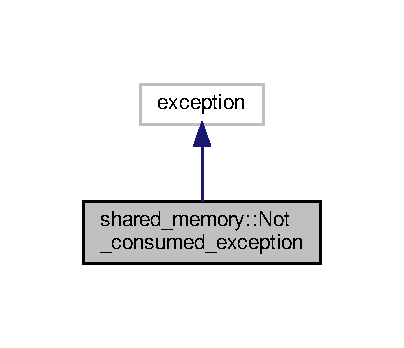
\includegraphics[width=194pt]{classshared__memory_1_1Not__consumed__exception__inherit__graph}
\end{center}
\end{figure}


Collaboration diagram for shared\+\_\+memory\+:\+:Not\+\_\+consumed\+\_\+exception\+:
\nopagebreak
\begin{figure}[H]
\begin{center}
\leavevmode
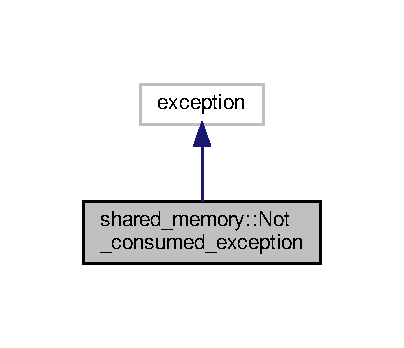
\includegraphics[width=194pt]{classshared__memory_1_1Not__consumed__exception__coll__graph}
\end{center}
\end{figure}
\subsection*{Public Member Functions}
\begin{DoxyCompactItemize}
\item 
\mbox{\Hypertarget{classshared__memory_1_1Not__consumed__exception_a10634d3dd5cb672f549205540fdd26a7}\label{classshared__memory_1_1Not__consumed__exception_a10634d3dd5cb672f549205540fdd26a7}} 
{\bfseries Not\+\_\+consumed\+\_\+exception} (int missed\+\_\+id)
\item 
\mbox{\Hypertarget{classshared__memory_1_1Not__consumed__exception_ae0055624cadbf945771291d61e5cb8a9}\label{classshared__memory_1_1Not__consumed__exception_ae0055624cadbf945771291d61e5cb8a9}} 
const char $\ast$ {\bfseries what} () const  throw ()
\end{DoxyCompactItemize}
\subsection*{Private Attributes}
\begin{DoxyCompactItemize}
\item 
\mbox{\Hypertarget{classshared__memory_1_1Not__consumed__exception_af35506334fcf23eae0ccfe101a2fdb9c}\label{classshared__memory_1_1Not__consumed__exception_af35506334fcf23eae0ccfe101a2fdb9c}} 
std\+::string {\bfseries error\+\_\+message\+\_\+}
\end{DoxyCompactItemize}


The documentation for this class was generated from the following files\+:\begin{DoxyCompactItemize}
\item 
include/shared\+\_\+memory/\hyperlink{exceptions_8h}{exceptions.\+h}\item 
src/\hyperlink{exceptions_8cpp}{exceptions.\+cpp}\end{DoxyCompactItemize}

\hypertarget{classshared__memory_1_1SegmentInfo}{}\section{shared\+\_\+memory\+:\+:Segment\+Info Class Reference}
\label{classshared__memory_1_1SegmentInfo}\index{shared\+\_\+memory\+::\+Segment\+Info@{shared\+\_\+memory\+::\+Segment\+Info}}


encapsulate information related to a shared memory segment  




{\ttfamily \#include $<$segment\+\_\+info.\+hpp$>$}

\subsection*{Public Member Functions}
\begin{DoxyCompactItemize}
\item 
\hyperlink{classshared__memory_1_1SegmentInfo_a254ed3b9d7e7e69a6888c9927504fe3b}{Segment\+Info} (boost\+::interprocess\+::managed\+\_\+shared\+\_\+memory \&msm)\hypertarget{classshared__memory_1_1SegmentInfo_a254ed3b9d7e7e69a6888c9927504fe3b}{}\label{classshared__memory_1_1SegmentInfo_a254ed3b9d7e7e69a6888c9927504fe3b}

\begin{DoxyCompactList}\small\item\em introspection of the shared memory segment \end{DoxyCompactList}\item 
uint \hyperlink{classshared__memory_1_1SegmentInfo_a0ab35167b7075c39adc5493511104b09}{get\+\_\+size} () const \hypertarget{classshared__memory_1_1SegmentInfo_a0ab35167b7075c39adc5493511104b09}{}\label{classshared__memory_1_1SegmentInfo_a0ab35167b7075c39adc5493511104b09}

\begin{DoxyCompactList}\small\item\em total size of the segment \end{DoxyCompactList}\item 
uint \hyperlink{classshared__memory_1_1SegmentInfo_aa91bb7d043ff723bc134fd4bcf38f718}{get\+\_\+free\+\_\+memory} () const \hypertarget{classshared__memory_1_1SegmentInfo_aa91bb7d043ff723bc134fd4bcf38f718}{}\label{classshared__memory_1_1SegmentInfo_aa91bb7d043ff723bc134fd4bcf38f718}

\begin{DoxyCompactList}\small\item\em free memory of the segment \end{DoxyCompactList}\item 
uint \hyperlink{classshared__memory_1_1SegmentInfo_a4c9c901d3220009dfb73fec4b0592a64}{get\+\_\+used\+\_\+memory} () const \hypertarget{classshared__memory_1_1SegmentInfo_a4c9c901d3220009dfb73fec4b0592a64}{}\label{classshared__memory_1_1SegmentInfo_a4c9c901d3220009dfb73fec4b0592a64}

\begin{DoxyCompactList}\small\item\em used memory of the segment \end{DoxyCompactList}\item 
bool \hyperlink{classshared__memory_1_1SegmentInfo_ace1754181cbe2be66e2eaebac7342795}{has\+\_\+issues} () const \hypertarget{classshared__memory_1_1SegmentInfo_ace1754181cbe2be66e2eaebac7342795}{}\label{classshared__memory_1_1SegmentInfo_ace1754181cbe2be66e2eaebac7342795}

\begin{DoxyCompactList}\small\item\em report on the status of the internal structures of the segment \end{DoxyCompactList}\item 
uint \hyperlink{classshared__memory_1_1SegmentInfo_aa1ecf75582e0df02205ad80c2797bc94}{nb\+\_\+objects} () const \hypertarget{classshared__memory_1_1SegmentInfo_aa1ecf75582e0df02205ad80c2797bc94}{}\label{classshared__memory_1_1SegmentInfo_aa1ecf75582e0df02205ad80c2797bc94}

\begin{DoxyCompactList}\small\item\em number of objects allocated in the segment \end{DoxyCompactList}\item 
void \hyperlink{classshared__memory_1_1SegmentInfo_a821eb6fc85451b03ea862e4cf5d6890c}{print} () const \hypertarget{classshared__memory_1_1SegmentInfo_a821eb6fc85451b03ea862e4cf5d6890c}{}\label{classshared__memory_1_1SegmentInfo_a821eb6fc85451b03ea862e4cf5d6890c}

\begin{DoxyCompactList}\small\item\em print in the terminal informations about the segment \end{DoxyCompactList}\end{DoxyCompactItemize}
\subsection*{Private Attributes}
\begin{DoxyCompactItemize}
\item 
uint {\bfseries size\+\_\+}\hypertarget{classshared__memory_1_1SegmentInfo_a87f1d90b4bfefd07945ba0e7d42959f4}{}\label{classshared__memory_1_1SegmentInfo_a87f1d90b4bfefd07945ba0e7d42959f4}

\item 
uint {\bfseries free\+\_\+memory\+\_\+}\hypertarget{classshared__memory_1_1SegmentInfo_ab1b9e3b023e45ccb327e7322d9dde554}{}\label{classshared__memory_1_1SegmentInfo_ab1b9e3b023e45ccb327e7322d9dde554}

\item 
bool {\bfseries has\+\_\+issues\+\_\+}\hypertarget{classshared__memory_1_1SegmentInfo_a727ff0d1a39302da90b26207de2ffc26}{}\label{classshared__memory_1_1SegmentInfo_a727ff0d1a39302da90b26207de2ffc26}

\item 
uint {\bfseries nb\+\_\+objects\+\_\+}\hypertarget{classshared__memory_1_1SegmentInfo_a56992f58b9b7c0bebbbff56d85a95a4b}{}\label{classshared__memory_1_1SegmentInfo_a56992f58b9b7c0bebbbff56d85a95a4b}

\end{DoxyCompactItemize}


\subsection{Detailed Description}
encapsulate information related to a shared memory segment 

The documentation for this class was generated from the following files\+:\begin{DoxyCompactItemize}
\item 
include/shared\+\_\+memory/segment\+\_\+info.\+hpp\item 
src/segment\+\_\+info.\+cpp\end{DoxyCompactItemize}

\hypertarget{classSerializable}{}\section{Serializable$<$ S\+I\+ZE $>$ Class Template Reference}
\label{classSerializable}\index{Serializable$<$ S\+I\+Z\+E $>$@{Serializable$<$ S\+I\+Z\+E $>$}}
\subsection*{Public Member Functions}
\begin{DoxyCompactItemize}
\item 
\mbox{\Hypertarget{classSerializable_a2db7fcfa31d5802fa8c889c41a2295b9}\label{classSerializable_a2db7fcfa31d5802fa8c889c41a2295b9}} 
void {\bfseries set} (int index, double v)
\item 
\mbox{\Hypertarget{classSerializable_a5f762ded2b44a416b362f6dfd9cf9976}\label{classSerializable_a5f762ded2b44a416b362f6dfd9cf9976}} 
double {\bfseries get} (int index)
\item 
\mbox{\Hypertarget{classSerializable_a442df4ac2ecad585776f620405b8ce0e}\label{classSerializable_a442df4ac2ecad585776f620405b8ce0e}} 
{\footnotesize template$<$class Archive $>$ }\\void {\bfseries serialize} (Archive \&archive)
\end{DoxyCompactItemize}
\subsection*{Private Types}
\begin{DoxyCompactItemize}
\item 
\mbox{\Hypertarget{classSerializable_a41015ba50b004943be3691039863377e}\label{classSerializable_a41015ba50b004943be3691039863377e}} 
typedef Eigen\+::\+Matrix$<$ double, S\+I\+ZE, 1 $>$ {\bfseries Vector}
\end{DoxyCompactItemize}
\subsection*{Private Attributes}
\begin{DoxyCompactItemize}
\item 
\mbox{\Hypertarget{classSerializable_abb77ae537c25b7941e041c3239f0085d}\label{classSerializable_abb77ae537c25b7941e041c3239f0085d}} 
double {\bfseries serialized\+\_\+v\+\_\+} \mbox{[}S\+I\+ZE\mbox{]}
\item 
\mbox{\Hypertarget{classSerializable_af836042e597c021ae7cbb1699c4de2e9}\label{classSerializable_af836042e597c021ae7cbb1699c4de2e9}} 
Eigen\+::\+Map$<$ Vector $>$ {\bfseries map\+\_\+}
\end{DoxyCompactItemize}


The documentation for this class was generated from the following file\+:\begin{DoxyCompactItemize}
\item 
demos/demo\+\_\+eigen.\+cpp\end{DoxyCompactItemize}

\hypertarget{classshared__memory_1_1Serializable__exchange}{}\section{shared\+\_\+memory\+:\+:Serializable\+\_\+exchange$<$ Serializable $>$ Class Template Reference}
\label{classshared__memory_1_1Serializable__exchange}\index{shared\+\_\+memory\+::\+Serializable\+\_\+exchange$<$ Serializable $>$@{shared\+\_\+memory\+::\+Serializable\+\_\+exchange$<$ Serializable $>$}}
\subsection*{Public Member Functions}
\begin{DoxyCompactItemize}
\item 
\mbox{\Hypertarget{classshared__memory_1_1Serializable__exchange_acb92a032cbc772e4d327d98208b214d3}\label{classshared__memory_1_1Serializable__exchange_acb92a032cbc772e4d327d98208b214d3}} 
{\bfseries Serializable\+\_\+exchange} (std\+::string segment\+\_\+id, std\+::string object\+\_\+id)
\item 
\mbox{\Hypertarget{classshared__memory_1_1Serializable__exchange_a29943c12f26bbd6e876b979d366fd110}\label{classshared__memory_1_1Serializable__exchange_a29943c12f26bbd6e876b979d366fd110}} 
void {\bfseries set} (const \hyperlink{classSerializable}{Serializable} \&serializable)
\item 
\mbox{\Hypertarget{classshared__memory_1_1Serializable__exchange_a3b69842f01b73a15bfefed264b8e3dd3}\label{classshared__memory_1_1Serializable__exchange_a3b69842f01b73a15bfefed264b8e3dd3}} 
void {\bfseries read} (\hyperlink{classSerializable}{Serializable} \&serializable)
\end{DoxyCompactItemize}
\subsection*{Private Attributes}
\begin{DoxyCompactItemize}
\item 
\mbox{\Hypertarget{classshared__memory_1_1Serializable__exchange_a495d9d0320ec199625deed0f1cd0ea20}\label{classshared__memory_1_1Serializable__exchange_a495d9d0320ec199625deed0f1cd0ea20}} 
std\+::string {\bfseries segment\+\_\+id\+\_\+}
\item 
\mbox{\Hypertarget{classshared__memory_1_1Serializable__exchange_a21968aa2fbfc11fa6ecc298320ebfb9a}\label{classshared__memory_1_1Serializable__exchange_a21968aa2fbfc11fa6ecc298320ebfb9a}} 
std\+::string {\bfseries object\+\_\+id\+\_\+}
\item 
\mbox{\Hypertarget{classshared__memory_1_1Serializable__exchange_a1923d2803a05846f61ee4738dac10674}\label{classshared__memory_1_1Serializable__exchange_a1923d2803a05846f61ee4738dac10674}} 
double $\ast$ {\bfseries data\+\_\+}
\end{DoxyCompactItemize}


The documentation for this class was generated from the following files\+:\begin{DoxyCompactItemize}
\item 
include/shared\+\_\+memory/\hyperlink{serializable__exchange_8hpp}{serializable\+\_\+exchange.\+hpp}\item 
include/shared\+\_\+memory/\hyperlink{serializable__exchange_8hxx}{serializable\+\_\+exchange.\+hxx}\end{DoxyCompactItemize}

\hypertarget{classSerializableExample}{}\section{Serializable\+Example Class Reference}
\label{classSerializableExample}\index{Serializable\+Example@{Serializable\+Example}}
\subsection*{Public Member Functions}
\begin{DoxyCompactItemize}
\item 
\mbox{\Hypertarget{classSerializableExample_a020d465dad63e984c2d665f5e59f7b85}\label{classSerializableExample_a020d465dad63e984c2d665f5e59f7b85}} 
{\bfseries Serializable\+Example} (int i1, int i2, double d1)
\item 
\mbox{\Hypertarget{classSerializableExample_ad31bb675456f6d5ff330c0a9ed44935f}\label{classSerializableExample_ad31bb675456f6d5ff330c0a9ed44935f}} 
void {\bfseries add} (int value)
\item 
\mbox{\Hypertarget{classSerializableExample_abd83ad2d93905e446c27faa83ccc27c4}\label{classSerializableExample_abd83ad2d93905e446c27faa83ccc27c4}} 
{\footnotesize template$<$class Archive $>$ }\\void {\bfseries serialize} (Archive \&archive)
\item 
\mbox{\Hypertarget{classSerializableExample_a045de0e6c3f89f14f0b088dd8978bce2}\label{classSerializableExample_a045de0e6c3f89f14f0b088dd8978bce2}} 
void {\bfseries print} ()
\end{DoxyCompactItemize}
\subsection*{Private Attributes}
\begin{DoxyCompactItemize}
\item 
\mbox{\Hypertarget{classSerializableExample_ab92737737108ec75894cdd774f382456}\label{classSerializableExample_ab92737737108ec75894cdd774f382456}} 
int {\bfseries i1\+\_\+}
\item 
\mbox{\Hypertarget{classSerializableExample_ac5b8225f7afd034537b83b9556f6e7ed}\label{classSerializableExample_ac5b8225f7afd034537b83b9556f6e7ed}} 
int {\bfseries i2\+\_\+}
\item 
\mbox{\Hypertarget{classSerializableExample_a6e0725b030db00c68689de4f2d23edfe}\label{classSerializableExample_a6e0725b030db00c68689de4f2d23edfe}} 
double {\bfseries d1\+\_\+}
\item 
\mbox{\Hypertarget{classSerializableExample_a6704295d511ce08e60005e153ca39b9a}\label{classSerializableExample_a6704295d511ce08e60005e153ca39b9a}} 
std\+::vector$<$ int $>$ {\bfseries v\+\_\+}
\end{DoxyCompactItemize}


The documentation for this class was generated from the following file\+:\begin{DoxyCompactItemize}
\item 
demos/serialization.\+cpp\end{DoxyCompactItemize}

\hypertarget{classshared__memory_1_1Serializer}{}\section{shared\+\_\+memory\+:\+:Serializer$<$ Serializable $>$ Class Template Reference}
\label{classshared__memory_1_1Serializer}\index{shared\+\_\+memory\+::\+Serializer$<$ Serializable $>$@{shared\+\_\+memory\+::\+Serializer$<$ Serializable $>$}}
\subsection*{Public Member Functions}
\begin{DoxyCompactItemize}
\item 
const std\+::string \& \hyperlink{classshared__memory_1_1Serializer_a61ea01a0e5e28fc24c9274455050b1c1}{serialize} (const \hyperlink{classSerializable}{Serializable} \&serializable)
\begin{DoxyCompactList}\small\item\em serialize an (almost) arbitrary instance to a string. \end{DoxyCompactList}\item 
void \hyperlink{classshared__memory_1_1Serializer_a8f674c9b3a7c053403112d2fad4e09a9}{deserialize} (const std\+::string \&data, \hyperlink{classSerializable}{Serializable} \&serializable)
\begin{DoxyCompactList}\small\item\em Restore the instance of serializable based on the string data, which should have been generated via the serialize function. \end{DoxyCompactList}\end{DoxyCompactItemize}
\subsection*{Static Public Member Functions}
\begin{DoxyCompactItemize}
\item 
static int \hyperlink{classshared__memory_1_1Serializer_af5edd0af254d6061e8e18c0bbec10aa9}{serializable\+\_\+size} ()
\begin{DoxyCompactList}\small\item\em Returns the serialized size (i.\+e. \end{DoxyCompactList}\end{DoxyCompactItemize}
\subsection*{Private Attributes}
\begin{DoxyCompactItemize}
\item 
\mbox{\Hypertarget{classshared__memory_1_1Serializer_ad1fb7ce2b9dfde8e609aa770a3f97e72}\label{classshared__memory_1_1Serializer_ad1fb7ce2b9dfde8e609aa770a3f97e72}} 
std\+::string {\bfseries data\+\_\+}
\end{DoxyCompactItemize}


\subsection{Member Function Documentation}
\mbox{\Hypertarget{classshared__memory_1_1Serializer_a8f674c9b3a7c053403112d2fad4e09a9}\label{classshared__memory_1_1Serializer_a8f674c9b3a7c053403112d2fad4e09a9}} 
\index{shared\+\_\+memory\+::\+Serializer@{shared\+\_\+memory\+::\+Serializer}!deserialize@{deserialize}}
\index{deserialize@{deserialize}!shared\+\_\+memory\+::\+Serializer@{shared\+\_\+memory\+::\+Serializer}}
\subsubsection{\texorpdfstring{deserialize()}{deserialize()}}
{\footnotesize\ttfamily template$<$class Serializable$>$ \\
void \hyperlink{classshared__memory_1_1Serializer}{shared\+\_\+memory\+::\+Serializer}$<$ \hyperlink{classSerializable}{Serializable} $>$\+::deserialize (\begin{DoxyParamCaption}\item[{const std\+::string \&}]{data,  }\item[{\hyperlink{classSerializable}{Serializable} \&}]{serializable }\end{DoxyParamCaption})}



Restore the instance of serializable based on the string data, which should have been generated via the serialize function. 


\begin{DoxyParams}{Parameters}
{\em the} & serialized instance \\
\hline
{\em instance} & of \hyperlink{classSerializable}{Serializable} to be restored \\
\hline
\end{DoxyParams}
\mbox{\Hypertarget{classshared__memory_1_1Serializer_af5edd0af254d6061e8e18c0bbec10aa9}\label{classshared__memory_1_1Serializer_af5edd0af254d6061e8e18c0bbec10aa9}} 
\index{shared\+\_\+memory\+::\+Serializer@{shared\+\_\+memory\+::\+Serializer}!serializable\+\_\+size@{serializable\+\_\+size}}
\index{serializable\+\_\+size@{serializable\+\_\+size}!shared\+\_\+memory\+::\+Serializer@{shared\+\_\+memory\+::\+Serializer}}
\subsubsection{\texorpdfstring{serializable\+\_\+size()}{serializable\_size()}}
{\footnotesize\ttfamily template$<$class Serializable $>$ \\
int \hyperlink{classshared__memory_1_1Serializer}{shared\+\_\+memory\+::\+Serializer}$<$ \hyperlink{classSerializable}{Serializable} $>$\+::serializable\+\_\+size (\begin{DoxyParamCaption}{ }\end{DoxyParamCaption})\hspace{0.3cm}{\ttfamily [static]}}



Returns the serialized size (i.\+e. 

the size of the string) of an instance of \hyperlink{classSerializable}{Serializable} \mbox{\Hypertarget{classshared__memory_1_1Serializer_a61ea01a0e5e28fc24c9274455050b1c1}\label{classshared__memory_1_1Serializer_a61ea01a0e5e28fc24c9274455050b1c1}} 
\index{shared\+\_\+memory\+::\+Serializer@{shared\+\_\+memory\+::\+Serializer}!serialize@{serialize}}
\index{serialize@{serialize}!shared\+\_\+memory\+::\+Serializer@{shared\+\_\+memory\+::\+Serializer}}
\subsubsection{\texorpdfstring{serialize()}{serialize()}}
{\footnotesize\ttfamily template$<$class Serializable$>$ \\
const std\+::string \& \hyperlink{classshared__memory_1_1Serializer}{shared\+\_\+memory\+::\+Serializer}$<$ \hyperlink{classSerializable}{Serializable} $>$\+::serialize (\begin{DoxyParamCaption}\item[{const \hyperlink{classSerializable}{Serializable} \&}]{serializable }\end{DoxyParamCaption})}



serialize an (almost) arbitrary instance to a string. 

The method uses cereal internally and the instance must implement a serialize function. See for details\+: \href{https://uscilab.github.io/cereal/}{\tt https\+://uscilab.\+github.\+io/cereal/} Supplementary requirements\+:
\begin{DoxyItemize}
\item \hyperlink{classSerializable}{Serializable} must also have a default constructor.
\item All instances of \hyperlink{classSerializable}{Serializable} must be of the same size. (e.\+g. vectors must be of fixed size) The generated and returned string is a private member of the \hyperlink{classshared__memory_1_1Serializer}{Serializer} instance. Successive calls to serialize overwrite this string. 
\begin{DoxyParams}{Parameters}
{\em instance} & to serialize to a string \\
\hline
\end{DoxyParams}

\end{DoxyItemize}

The documentation for this class was generated from the following files\+:\begin{DoxyCompactItemize}
\item 
include/shared\+\_\+memory/serializer.\+hpp\item 
include/shared\+\_\+memory/serializer.\+hxx\end{DoxyCompactItemize}

\hypertarget{classshared__memory_1_1SharedMemorySegment}{}\section{shared\+\_\+memory\+:\+:Shared\+Memory\+Segment Class Reference}
\label{classshared__memory_1_1SharedMemorySegment}\index{shared\+\_\+memory\+::\+Shared\+Memory\+Segment@{shared\+\_\+memory\+::\+Shared\+Memory\+Segment}}


The \hyperlink{classshared__memory_1_1SharedMemorySegment}{Shared\+Memory\+Segment} contains the pointers of the shared objects in on shared memrory segment.  




{\ttfamily \#include $<$shared\+\_\+memory.\+hpp$>$}

\subsection*{Public Member Functions}
\begin{DoxyCompactItemize}
\item 
\mbox{\Hypertarget{classshared__memory_1_1SharedMemorySegment_ae984411227bd175e684f90c9c28c976c}\label{classshared__memory_1_1SharedMemorySegment_ae984411227bd175e684f90c9c28c976c}} 
\hyperlink{classshared__memory_1_1SharedMemorySegment_ae984411227bd175e684f90c9c28c976c}{Shared\+Memory\+Segment} (std\+::string segment\+\_\+id, bool clear\+\_\+upon\+\_\+destruction)
\begin{DoxyCompactList}\small\item\em \hyperlink{classshared__memory_1_1SharedMemorySegment}{Shared\+Memory\+Segment} constructor. \end{DoxyCompactList}\item 
\mbox{\Hypertarget{classshared__memory_1_1SharedMemorySegment_a9f02fd9f35950df5f6ce7ceaba5fbb53}\label{classshared__memory_1_1SharedMemorySegment_a9f02fd9f35950df5f6ce7ceaba5fbb53}} 
\hyperlink{classshared__memory_1_1SharedMemorySegment_a9f02fd9f35950df5f6ce7ceaba5fbb53}{$\sim$\+Shared\+Memory\+Segment} ()
\begin{DoxyCompactList}\small\item\em \hyperlink{classshared__memory_1_1SharedMemorySegment}{Shared\+Memory\+Segment} destructor. \end{DoxyCompactList}\item 
\mbox{\Hypertarget{classshared__memory_1_1SharedMemorySegment_a0224739cd729dfb249c3d7882463e5eb}\label{classshared__memory_1_1SharedMemorySegment_a0224739cd729dfb249c3d7882463e5eb}} 
void \hyperlink{classshared__memory_1_1SharedMemorySegment_a0224739cd729dfb249c3d7882463e5eb}{clear\+\_\+memory} ()
\begin{DoxyCompactList}\small\item\em clear\+\_\+memory free the shared memory \end{DoxyCompactList}\item 
{\footnotesize template$<$typename Elem\+Type $>$ }\\void \hyperlink{classshared__memory_1_1SharedMemorySegment_ad73b5160f713c9a78e67c4b8590d8729}{get\+\_\+object} (const std\+::string \&object\+\_\+id, std\+::pair$<$ Elem\+Type $\ast$, std\+::size\+\_\+t $>$ \&get\+\_\+)
\begin{DoxyCompactList}\small\item\em get\+\_\+object registers the object in the current struc and in the shared memory once only. \end{DoxyCompactList}\item 
void \hyperlink{classshared__memory_1_1SharedMemorySegment_a17aa3bfe778e05b543415b1e5137a26b}{get\+\_\+object} (const std\+::string \&object\+\_\+id, std\+::string \&get\+\_\+)
\begin{DoxyCompactList}\small\item\em get\+\_\+object registers the object in the current struc and in the shared memory once only. \end{DoxyCompactList}\item 
{\footnotesize template$<$typename Elem\+Type $>$ }\\void \hyperlink{classshared__memory_1_1SharedMemorySegment_a16e6213d7dd1984799bbd8fbe14225dc}{set\+\_\+object} (const std\+::string \&object\+\_\+id, const std\+::pair$<$ const Elem\+Type $\ast$, std\+::size\+\_\+t $>$ \&set\+\_\+)
\begin{DoxyCompactList}\small\item\em set\+\_\+object registers the object in the current struc and in the shared memory once only. \end{DoxyCompactList}\item 
{\footnotesize template$<$typename Elem\+Type $>$ }\\bool \hyperlink{classshared__memory_1_1SharedMemorySegment_a6987e8225fd20dbab12e5bb3f5305b75}{register\+\_\+object} (const std\+::string \&object\+\_\+id, const std\+::pair$<$ Elem\+Type $\ast$, std\+::size\+\_\+t $>$ \&obj\+\_\+)
\begin{DoxyCompactList}\small\item\em register\+\_\+object registers the object in the segment uniquely. \end{DoxyCompactList}\item 
{\footnotesize template$<$typename Elem\+Type $>$ }\\bool \hyperlink{classshared__memory_1_1SharedMemorySegment_a830fee375b183642b999f6a64240f280}{register\+\_\+object\+\_\+read\+\_\+only} (const std\+::string \&object\+\_\+id)
\begin{DoxyCompactList}\small\item\em register\+\_\+object\+\_\+read\+\_\+only registers the object in the segment uniquely. \end{DoxyCompactList}\item 
{\footnotesize template$<$typename Elem\+Type $>$ }\\void \hyperlink{classshared__memory_1_1SharedMemorySegment_abc658e54589c81e89b147f0b3fbd67b8}{delete\+\_\+object} (const std\+::string \&object\+\_\+id)
\begin{DoxyCompactList}\small\item\em delete\+\_\+object delete and object from the shared memory. \end{DoxyCompactList}\item 
\mbox{\Hypertarget{classshared__memory_1_1SharedMemorySegment_ac8bbbc98968a8a2b3fe35c50e0768d8f}\label{classshared__memory_1_1SharedMemorySegment_ac8bbbc98968a8a2b3fe35c50e0768d8f}} 
void \hyperlink{classshared__memory_1_1SharedMemorySegment_ac8bbbc98968a8a2b3fe35c50e0768d8f}{create\+\_\+mutex} ()
\begin{DoxyCompactList}\small\item\em create\+\_\+mutex small factory that allow to make sure that the mutex is created. \end{DoxyCompactList}\item 
\mbox{\Hypertarget{classshared__memory_1_1SharedMemorySegment_a64d69c4965cd448040bc20e4f9009abc}\label{classshared__memory_1_1SharedMemorySegment_a64d69c4965cd448040bc20e4f9009abc}} 
void \hyperlink{classshared__memory_1_1SharedMemorySegment_a64d69c4965cd448040bc20e4f9009abc}{destroy\+\_\+mutex} ()
\begin{DoxyCompactList}\small\item\em destroy\+\_\+mutex small destructor of the mutext to make sure that it is unlock at critical time. \end{DoxyCompactList}\item 
bool \hyperlink{classshared__memory_1_1SharedMemorySegment_ae7a86bba2f8158917b48c0bd3a7bdf9b}{is\+\_\+object\+\_\+registered} (const std\+::string \&object\+\_\+id)
\begin{DoxyCompactList}\small\item\em is\+\_\+object\+\_\+registered used to check if the object has been registered or not. \end{DoxyCompactList}\item 
void \hyperlink{classshared__memory_1_1SharedMemorySegment_ae2eb51704f44076db6ce79054e9d2572}{set\+\_\+clear\+\_\+upon\+\_\+destruction} (const bool clear\+\_\+upon\+\_\+destruction)
\begin{DoxyCompactList}\small\item\em set\+\_\+clear\+\_\+upon\+\_\+destruction is a standard setter \end{DoxyCompactList}\item 
const std\+::string \& \hyperlink{classshared__memory_1_1SharedMemorySegment_ab7f1f01a94d4e45ed907be9bcdb71a24}{get\+\_\+segment\+\_\+id} ()
\begin{DoxyCompactList}\small\item\em get\+\_\+segment\+\_\+id is a standard getter \end{DoxyCompactList}\item 
\mbox{\Hypertarget{classshared__memory_1_1SharedMemorySegment_aa742cf04463a94a51239b96de2da6947}\label{classshared__memory_1_1SharedMemorySegment_aa742cf04463a94a51239b96de2da6947}} 
\hyperlink{classshared__memory_1_1SegmentInfo}{Segment\+Info} \hyperlink{classshared__memory_1_1SharedMemorySegment_aa742cf04463a94a51239b96de2da6947}{get\+\_\+info} ()
\begin{DoxyCompactList}\small\item\em performs introspection on the segment and return related information \end{DoxyCompactList}\end{DoxyCompactItemize}
\subsection*{Public Attributes}
\begin{DoxyCompactItemize}
\item 
\mbox{\Hypertarget{classshared__memory_1_1SharedMemorySegment_a9e72fec52b3c76b9c2b0809b40b4e11d}\label{classshared__memory_1_1SharedMemorySegment_a9e72fec52b3c76b9c2b0809b40b4e11d}} 
boost\+::interprocess\+::interprocess\+\_\+mutex $\ast$ \hyperlink{classshared__memory_1_1SharedMemorySegment_a9e72fec52b3c76b9c2b0809b40b4e11d}{mutex\+\_\+}
\begin{DoxyCompactList}\small\item\em mutex\+\_\+ this mutex secure A\+LL the shared memory. \end{DoxyCompactList}\end{DoxyCompactItemize}
\subsection*{Private Attributes}
\begin{DoxyCompactItemize}
\item 
\mbox{\Hypertarget{classshared__memory_1_1SharedMemorySegment_af775c0982687b6e9bc9856b21aa1e009}\label{classshared__memory_1_1SharedMemorySegment_af775c0982687b6e9bc9856b21aa1e009}} 
boost\+::interprocess\+::managed\+\_\+shared\+\_\+memory \hyperlink{classshared__memory_1_1SharedMemorySegment_af775c0982687b6e9bc9856b21aa1e009}{segment\+\_\+manager\+\_\+}
\begin{DoxyCompactList}\small\item\em shm\+\_\+segment is the boost object that manages the shared memory segment \end{DoxyCompactList}\item 
\hyperlink{namespaceshared__memory_ae50b2192256821112a69e47d5314b467}{Shm\+Objects} \hyperlink{classshared__memory_1_1SharedMemorySegment_a8c4d0eb6f2a620bf7e5b22a57c07380b}{objects\+\_\+}
\begin{DoxyCompactList}\small\item\em objects\+\_\+ are all the data stored in the segment. \end{DoxyCompactList}\item 
\mbox{\Hypertarget{classshared__memory_1_1SharedMemorySegment_a08408dc6b860388eb3b08e493f0188d9}\label{classshared__memory_1_1SharedMemorySegment_a08408dc6b860388eb3b08e493f0188d9}} 
std\+::string \hyperlink{classshared__memory_1_1SharedMemorySegment_a08408dc6b860388eb3b08e493f0188d9}{segment\+\_\+id\+\_\+}
\begin{DoxyCompactList}\small\item\em segment\+\_\+id\+\_\+ is the name of the segment inside the shared memory \end{DoxyCompactList}\item 
bool \hyperlink{classshared__memory_1_1SharedMemorySegment_af50ac70dca284926b15803f86958b220}{clear\+\_\+upon\+\_\+destruction\+\_\+}
\begin{DoxyCompactList}\small\item\em clear\+\_\+upon\+\_\+destruction\+\_\+ flag decides if the segment should be cleared upon destruction. \end{DoxyCompactList}\end{DoxyCompactItemize}


\subsection{Detailed Description}
The \hyperlink{classshared__memory_1_1SharedMemorySegment}{Shared\+Memory\+Segment} contains the pointers of the shared objects in on shared memrory segment. 

We use unamed mutext (interprocess\+\_\+mutex) and unamed condition variables (interprocess\+\_\+condition) to be able to instanciate them with classic pointers 

\subsection{Member Function Documentation}
\mbox{\Hypertarget{classshared__memory_1_1SharedMemorySegment_abc658e54589c81e89b147f0b3fbd67b8}\label{classshared__memory_1_1SharedMemorySegment_abc658e54589c81e89b147f0b3fbd67b8}} 
\index{shared\+\_\+memory\+::\+Shared\+Memory\+Segment@{shared\+\_\+memory\+::\+Shared\+Memory\+Segment}!delete\+\_\+object@{delete\+\_\+object}}
\index{delete\+\_\+object@{delete\+\_\+object}!shared\+\_\+memory\+::\+Shared\+Memory\+Segment@{shared\+\_\+memory\+::\+Shared\+Memory\+Segment}}
\subsubsection{\texorpdfstring{delete\+\_\+object()}{delete\_object()}}
{\footnotesize\ttfamily template$<$typename Elem\+Type $>$ \\
void shared\+\_\+memory\+::\+Shared\+Memory\+Segment\+::delete\+\_\+object (\begin{DoxyParamCaption}\item[{const std\+::string \&}]{object\+\_\+id }\end{DoxyParamCaption})}



delete\+\_\+object delete and object from the shared memory. 


\begin{DoxyParams}[1]{Parameters}
\mbox{\tt in}  & {\em object\+\_\+id} & the name of the object in the shared memory. \\
\hline
\end{DoxyParams}
\mbox{\Hypertarget{classshared__memory_1_1SharedMemorySegment_ad73b5160f713c9a78e67c4b8590d8729}\label{classshared__memory_1_1SharedMemorySegment_ad73b5160f713c9a78e67c4b8590d8729}} 
\index{shared\+\_\+memory\+::\+Shared\+Memory\+Segment@{shared\+\_\+memory\+::\+Shared\+Memory\+Segment}!get\+\_\+object@{get\+\_\+object}}
\index{get\+\_\+object@{get\+\_\+object}!shared\+\_\+memory\+::\+Shared\+Memory\+Segment@{shared\+\_\+memory\+::\+Shared\+Memory\+Segment}}
\subsubsection{\texorpdfstring{get\+\_\+object()}{get\_object()}\hspace{0.1cm}{\footnotesize\ttfamily [1/2]}}
{\footnotesize\ttfamily template$<$typename Elem\+Type $>$ \\
void shared\+\_\+memory\+::\+Shared\+Memory\+Segment\+::get\+\_\+object (\begin{DoxyParamCaption}\item[{const std\+::string \&}]{object\+\_\+id,  }\item[{std\+::pair$<$ Elem\+Type $\ast$, std\+::size\+\_\+t $>$ \&}]{get\+\_\+ }\end{DoxyParamCaption})}



get\+\_\+object registers the object in the current struc and in the shared memory once only. 

And returns the pointer to the object and its size. The size will be 1 for simple type and could greater to one for arrays. 
\begin{DoxyParams}[1]{Parameters}
\mbox{\tt in}  & {\em object\+\_\+id} & the name of the object in the shared memory. \\
\hline
\mbox{\tt in}  & {\em } & \\
\hline
\end{DoxyParams}
\mbox{\Hypertarget{classshared__memory_1_1SharedMemorySegment_a17aa3bfe778e05b543415b1e5137a26b}\label{classshared__memory_1_1SharedMemorySegment_a17aa3bfe778e05b543415b1e5137a26b}} 
\index{shared\+\_\+memory\+::\+Shared\+Memory\+Segment@{shared\+\_\+memory\+::\+Shared\+Memory\+Segment}!get\+\_\+object@{get\+\_\+object}}
\index{get\+\_\+object@{get\+\_\+object}!shared\+\_\+memory\+::\+Shared\+Memory\+Segment@{shared\+\_\+memory\+::\+Shared\+Memory\+Segment}}
\subsubsection{\texorpdfstring{get\+\_\+object()}{get\_object()}\hspace{0.1cm}{\footnotesize\ttfamily [2/2]}}
{\footnotesize\ttfamily void shared\+\_\+memory\+::\+Shared\+Memory\+Segment\+::get\+\_\+object (\begin{DoxyParamCaption}\item[{const std\+::string \&}]{object\+\_\+id,  }\item[{std\+::string \&}]{get\+\_\+ }\end{DoxyParamCaption})}



get\+\_\+object registers the object in the current struc and in the shared memory once only. 

And returns the pointer to the object and its size. The size will be 1 for simple type and could greater to one for arrays. 
\begin{DoxyParams}[1]{Parameters}
\mbox{\tt in}  & {\em object\+\_\+id} & the name of the object in the shared memory. \\
\hline
\mbox{\tt in}  & {\em } & \\
\hline
\end{DoxyParams}
\mbox{\Hypertarget{classshared__memory_1_1SharedMemorySegment_ab7f1f01a94d4e45ed907be9bcdb71a24}\label{classshared__memory_1_1SharedMemorySegment_ab7f1f01a94d4e45ed907be9bcdb71a24}} 
\index{shared\+\_\+memory\+::\+Shared\+Memory\+Segment@{shared\+\_\+memory\+::\+Shared\+Memory\+Segment}!get\+\_\+segment\+\_\+id@{get\+\_\+segment\+\_\+id}}
\index{get\+\_\+segment\+\_\+id@{get\+\_\+segment\+\_\+id}!shared\+\_\+memory\+::\+Shared\+Memory\+Segment@{shared\+\_\+memory\+::\+Shared\+Memory\+Segment}}
\subsubsection{\texorpdfstring{get\+\_\+segment\+\_\+id()}{get\_segment\_id()}}
{\footnotesize\ttfamily const std\+::string\& shared\+\_\+memory\+::\+Shared\+Memory\+Segment\+::get\+\_\+segment\+\_\+id (\begin{DoxyParamCaption}{ }\end{DoxyParamCaption})\hspace{0.3cm}{\ttfamily [inline]}}



get\+\_\+segment\+\_\+id is a standard getter 

\begin{DoxyReturn}{Returns}
the segment name 
\end{DoxyReturn}
\mbox{\Hypertarget{classshared__memory_1_1SharedMemorySegment_ae7a86bba2f8158917b48c0bd3a7bdf9b}\label{classshared__memory_1_1SharedMemorySegment_ae7a86bba2f8158917b48c0bd3a7bdf9b}} 
\index{shared\+\_\+memory\+::\+Shared\+Memory\+Segment@{shared\+\_\+memory\+::\+Shared\+Memory\+Segment}!is\+\_\+object\+\_\+registered@{is\+\_\+object\+\_\+registered}}
\index{is\+\_\+object\+\_\+registered@{is\+\_\+object\+\_\+registered}!shared\+\_\+memory\+::\+Shared\+Memory\+Segment@{shared\+\_\+memory\+::\+Shared\+Memory\+Segment}}
\subsubsection{\texorpdfstring{is\+\_\+object\+\_\+registered()}{is\_object\_registered()}}
{\footnotesize\ttfamily bool shared\+\_\+memory\+::\+Shared\+Memory\+Segment\+::is\+\_\+object\+\_\+registered (\begin{DoxyParamCaption}\item[{const std\+::string \&}]{object\+\_\+id }\end{DoxyParamCaption})\hspace{0.3cm}{\ttfamily [inline]}}



is\+\_\+object\+\_\+registered used to check if the object has been registered or not. 


\begin{DoxyParams}[1]{Parameters}
\mbox{\tt in}  & {\em object\+\_\+id} & the name of the object in the shared memory. \\
\hline
\end{DoxyParams}
\begin{DoxyReturn}{Returns}
true if it has been registered 
\end{DoxyReturn}
\mbox{\Hypertarget{classshared__memory_1_1SharedMemorySegment_a6987e8225fd20dbab12e5bb3f5305b75}\label{classshared__memory_1_1SharedMemorySegment_a6987e8225fd20dbab12e5bb3f5305b75}} 
\index{shared\+\_\+memory\+::\+Shared\+Memory\+Segment@{shared\+\_\+memory\+::\+Shared\+Memory\+Segment}!register\+\_\+object@{register\+\_\+object}}
\index{register\+\_\+object@{register\+\_\+object}!shared\+\_\+memory\+::\+Shared\+Memory\+Segment@{shared\+\_\+memory\+::\+Shared\+Memory\+Segment}}
\subsubsection{\texorpdfstring{register\+\_\+object()}{register\_object()}}
{\footnotesize\ttfamily template$<$typename Elem\+Type $>$ \\
bool shared\+\_\+memory\+::\+Shared\+Memory\+Segment\+::register\+\_\+object (\begin{DoxyParamCaption}\item[{const std\+::string \&}]{object\+\_\+id,  }\item[{const std\+::pair$<$ Elem\+Type $\ast$, std\+::size\+\_\+t $>$ \&}]{obj\+\_\+ }\end{DoxyParamCaption})}



register\+\_\+object registers the object in the segment uniquely. 


\begin{DoxyParams}{Parameters}
{\em object\+\_\+id} & is the name of the object to register. \\
\hline
{\em obj\+\_\+} & is the object to be registered. \\
\hline
\end{DoxyParams}
\begin{DoxyReturn}{Returns}
true of a new object has been registered 
\end{DoxyReturn}
\mbox{\Hypertarget{classshared__memory_1_1SharedMemorySegment_a830fee375b183642b999f6a64240f280}\label{classshared__memory_1_1SharedMemorySegment_a830fee375b183642b999f6a64240f280}} 
\index{shared\+\_\+memory\+::\+Shared\+Memory\+Segment@{shared\+\_\+memory\+::\+Shared\+Memory\+Segment}!register\+\_\+object\+\_\+read\+\_\+only@{register\+\_\+object\+\_\+read\+\_\+only}}
\index{register\+\_\+object\+\_\+read\+\_\+only@{register\+\_\+object\+\_\+read\+\_\+only}!shared\+\_\+memory\+::\+Shared\+Memory\+Segment@{shared\+\_\+memory\+::\+Shared\+Memory\+Segment}}
\subsubsection{\texorpdfstring{register\+\_\+object\+\_\+read\+\_\+only()}{register\_object\_read\_only()}}
{\footnotesize\ttfamily template$<$typename Elem\+Type $>$ \\
bool shared\+\_\+memory\+::\+Shared\+Memory\+Segment\+::register\+\_\+object\+\_\+read\+\_\+only (\begin{DoxyParamCaption}\item[{const std\+::string \&}]{object\+\_\+id }\end{DoxyParamCaption})}



register\+\_\+object\+\_\+read\+\_\+only registers the object in the segment uniquely. 


\begin{DoxyParams}{Parameters}
{\em object\+\_\+id} & is the name of the object to register \\
\hline
{\em obj\+\_\+} & is the object to be registered \\
\hline
\end{DoxyParams}
\begin{DoxyReturn}{Returns}
true of a new object has been registered 
\end{DoxyReturn}
\mbox{\Hypertarget{classshared__memory_1_1SharedMemorySegment_ae2eb51704f44076db6ce79054e9d2572}\label{classshared__memory_1_1SharedMemorySegment_ae2eb51704f44076db6ce79054e9d2572}} 
\index{shared\+\_\+memory\+::\+Shared\+Memory\+Segment@{shared\+\_\+memory\+::\+Shared\+Memory\+Segment}!set\+\_\+clear\+\_\+upon\+\_\+destruction@{set\+\_\+clear\+\_\+upon\+\_\+destruction}}
\index{set\+\_\+clear\+\_\+upon\+\_\+destruction@{set\+\_\+clear\+\_\+upon\+\_\+destruction}!shared\+\_\+memory\+::\+Shared\+Memory\+Segment@{shared\+\_\+memory\+::\+Shared\+Memory\+Segment}}
\subsubsection{\texorpdfstring{set\+\_\+clear\+\_\+upon\+\_\+destruction()}{set\_clear\_upon\_destruction()}}
{\footnotesize\ttfamily void shared\+\_\+memory\+::\+Shared\+Memory\+Segment\+::set\+\_\+clear\+\_\+upon\+\_\+destruction (\begin{DoxyParamCaption}\item[{const bool}]{clear\+\_\+upon\+\_\+destruction }\end{DoxyParamCaption})\hspace{0.3cm}{\ttfamily [inline]}}



set\+\_\+clear\+\_\+upon\+\_\+destruction is a standard setter 


\begin{DoxyParams}[1]{Parameters}
\mbox{\tt in}  & {\em clear\+\_\+upon\+\_\+destruction} & is the value to set \\
\hline
\end{DoxyParams}
\mbox{\Hypertarget{classshared__memory_1_1SharedMemorySegment_a16e6213d7dd1984799bbd8fbe14225dc}\label{classshared__memory_1_1SharedMemorySegment_a16e6213d7dd1984799bbd8fbe14225dc}} 
\index{shared\+\_\+memory\+::\+Shared\+Memory\+Segment@{shared\+\_\+memory\+::\+Shared\+Memory\+Segment}!set\+\_\+object@{set\+\_\+object}}
\index{set\+\_\+object@{set\+\_\+object}!shared\+\_\+memory\+::\+Shared\+Memory\+Segment@{shared\+\_\+memory\+::\+Shared\+Memory\+Segment}}
\subsubsection{\texorpdfstring{set\+\_\+object()}{set\_object()}}
{\footnotesize\ttfamily template$<$typename Elem\+Type $>$ \\
void shared\+\_\+memory\+::\+Shared\+Memory\+Segment\+::set\+\_\+object (\begin{DoxyParamCaption}\item[{const std\+::string \&}]{object\+\_\+id,  }\item[{const std\+::pair$<$ const Elem\+Type $\ast$, std\+::size\+\_\+t $>$ \&}]{set\+\_\+ }\end{DoxyParamCaption})}



set\+\_\+object registers the object in the current struc and in the shared memory once only. 

And returns the pointer to the object and its size. The size will be 1 for simple type and could greater to one for arrays. 
\begin{DoxyParams}[1]{Parameters}
\mbox{\tt in}  & {\em object\+\_\+id} & the name of the object in the shared memory. \\
\hline
\mbox{\tt in}  & {\em set\+\_\+} & the reference to the fetched object. \\
\hline
\end{DoxyParams}


\subsection{Member Data Documentation}
\mbox{\Hypertarget{classshared__memory_1_1SharedMemorySegment_af50ac70dca284926b15803f86958b220}\label{classshared__memory_1_1SharedMemorySegment_af50ac70dca284926b15803f86958b220}} 
\index{shared\+\_\+memory\+::\+Shared\+Memory\+Segment@{shared\+\_\+memory\+::\+Shared\+Memory\+Segment}!clear\+\_\+upon\+\_\+destruction\+\_\+@{clear\+\_\+upon\+\_\+destruction\+\_\+}}
\index{clear\+\_\+upon\+\_\+destruction\+\_\+@{clear\+\_\+upon\+\_\+destruction\+\_\+}!shared\+\_\+memory\+::\+Shared\+Memory\+Segment@{shared\+\_\+memory\+::\+Shared\+Memory\+Segment}}
\subsubsection{\texorpdfstring{clear\+\_\+upon\+\_\+destruction\+\_\+}{clear\_upon\_destruction\_}}
{\footnotesize\ttfamily bool shared\+\_\+memory\+::\+Shared\+Memory\+Segment\+::clear\+\_\+upon\+\_\+destruction\+\_\+\hspace{0.3cm}{\ttfamily [private]}}



clear\+\_\+upon\+\_\+destruction\+\_\+ flag decides if the segment should be cleared upon destruction. 

Usage\+: typically only one process should set this flag to true. \mbox{\Hypertarget{classshared__memory_1_1SharedMemorySegment_a8c4d0eb6f2a620bf7e5b22a57c07380b}\label{classshared__memory_1_1SharedMemorySegment_a8c4d0eb6f2a620bf7e5b22a57c07380b}} 
\index{shared\+\_\+memory\+::\+Shared\+Memory\+Segment@{shared\+\_\+memory\+::\+Shared\+Memory\+Segment}!objects\+\_\+@{objects\+\_\+}}
\index{objects\+\_\+@{objects\+\_\+}!shared\+\_\+memory\+::\+Shared\+Memory\+Segment@{shared\+\_\+memory\+::\+Shared\+Memory\+Segment}}
\subsubsection{\texorpdfstring{objects\+\_\+}{objects\_}}
{\footnotesize\ttfamily \hyperlink{namespaceshared__memory_ae50b2192256821112a69e47d5314b467}{Shm\+Objects} shared\+\_\+memory\+::\+Shared\+Memory\+Segment\+::objects\+\_\+\hspace{0.3cm}{\ttfamily [private]}}



objects\+\_\+ are all the data stored in the segment. 

W\+A\+R\+N\+I\+NG here we use void$\ast$ so the use of the set and get functions is the R\+E\+S\+P\+O\+N\+S\+A\+B\+I\+L\+I\+TY of the user.

The user is to use the S\+A\+ME type when calling set and get using the shared memory 

The documentation for this class was generated from the following files\+:\begin{DoxyCompactItemize}
\item 
include/shared\+\_\+memory/\hyperlink{shared__memory_8hpp}{shared\+\_\+memory.\+hpp}\item 
include/shared\+\_\+memory/\hyperlink{shared__memory_8hxx}{shared\+\_\+memory.\+hxx}\item 
src/\hyperlink{shared__memory_8cpp}{shared\+\_\+memory.\+cpp}\end{DoxyCompactItemize}

\hypertarget{structshared__memory_1_1ShmTypeHelper}{}\section{shared\+\_\+memory\+:\+:Shm\+Type\+Helper$<$ Elem\+Type $>$ Struct Template Reference}
\label{structshared__memory_1_1ShmTypeHelper}\index{shared\+\_\+memory\+::\+Shm\+Type\+Helper$<$ Elem\+Type $>$@{shared\+\_\+memory\+::\+Shm\+Type\+Helper$<$ Elem\+Type $>$}}


\hyperlink{structshared__memory_1_1ShmTypeHelper}{Shm\+Type\+Helper} is a small struct that allow the definition of templated typedef.  




{\ttfamily \#include $<$shared\+\_\+memory.\+hpp$>$}

\subsection*{Public Types}
\begin{DoxyCompactItemize}
\item 
\mbox{\Hypertarget{structshared__memory_1_1ShmTypeHelper_a8f19a7da45c3208eade1e5943588e5da}\label{structshared__memory_1_1ShmTypeHelper_a8f19a7da45c3208eade1e5943588e5da}} 
typedef boost\+::interprocess\+::allocator$<$ Elem\+Type, boost\+::interprocess\+::managed\+\_\+shared\+\_\+memory\+::segment\+\_\+manager $>$ \hyperlink{structshared__memory_1_1ShmTypeHelper_a8f19a7da45c3208eade1e5943588e5da}{Elem\+Type\+Allocator}
\begin{DoxyCompactList}\small\item\em Shmem\+Allocator typedef allows to create std\+::allocator with the boost interprocess library. \end{DoxyCompactList}\item 
\mbox{\Hypertarget{structshared__memory_1_1ShmTypeHelper_a935d582ba7497fea7a44a7e74ac9219e}\label{structshared__memory_1_1ShmTypeHelper_a935d582ba7497fea7a44a7e74ac9219e}} 
typedef boost\+::container\+::deque$<$ Elem\+Type, \hyperlink{structshared__memory_1_1ShmTypeHelper}{Shm\+Type\+Helper}$<$ Elem\+Type $>$\+::\hyperlink{structshared__memory_1_1ShmTypeHelper_a8f19a7da45c3208eade1e5943588e5da}{Elem\+Type\+Allocator} $>$ {\bfseries Shm\+Deque}
\item 
\mbox{\Hypertarget{structshared__memory_1_1ShmTypeHelper_a306bff24c9271b479fdfd238bef10580}\label{structshared__memory_1_1ShmTypeHelper_a306bff24c9271b479fdfd238bef10580}} 
typedef boost\+::container\+::vector$<$ Elem\+Type, \hyperlink{structshared__memory_1_1ShmTypeHelper}{Shm\+Type\+Helper}$<$ Elem\+Type $>$\+::\hyperlink{structshared__memory_1_1ShmTypeHelper_a8f19a7da45c3208eade1e5943588e5da}{Elem\+Type\+Allocator} $>$ {\bfseries Shm\+Vector}
\end{DoxyCompactItemize}


\subsection{Detailed Description}
\subsubsection*{template$<$typename Elem\+Type$>$\newline
struct shared\+\_\+memory\+::\+Shm\+Type\+Helper$<$ Elem\+Type $>$}

\hyperlink{structshared__memory_1_1ShmTypeHelper}{Shm\+Type\+Helper} is a small struct that allow the definition of templated typedef. 

The documentation for this struct was generated from the following file\+:\begin{DoxyCompactItemize}
\item 
include/shared\+\_\+memory/\hyperlink{shared__memory_8hpp}{shared\+\_\+memory.\+hpp}\end{DoxyCompactItemize}

\hypertarget{classshared__memory_1_1Unexpected__map__key}{}\section{shared\+\_\+memory\+:\+:Unexpected\+\_\+map\+\_\+key$<$ Key $>$ Class Template Reference}
\label{classshared__memory_1_1Unexpected__map__key}\index{shared\+\_\+memory\+::\+Unexpected\+\_\+map\+\_\+key$<$ Key $>$@{shared\+\_\+memory\+::\+Unexpected\+\_\+map\+\_\+key$<$ Key $>$}}


Inheritance diagram for shared\+\_\+memory\+:\+:Unexpected\+\_\+map\+\_\+key$<$ Key $>$\+:
\nopagebreak
\begin{figure}[H]
\begin{center}
\leavevmode
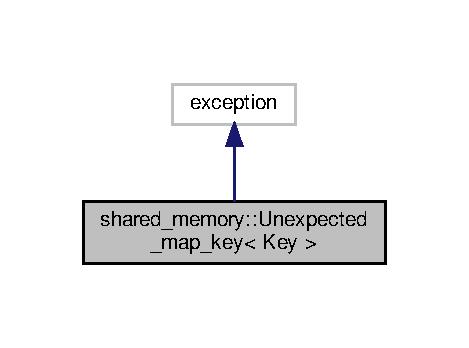
\includegraphics[width=225pt]{classshared__memory_1_1Unexpected__map__key__inherit__graph}
\end{center}
\end{figure}


Collaboration diagram for shared\+\_\+memory\+:\+:Unexpected\+\_\+map\+\_\+key$<$ Key $>$\+:
\nopagebreak
\begin{figure}[H]
\begin{center}
\leavevmode
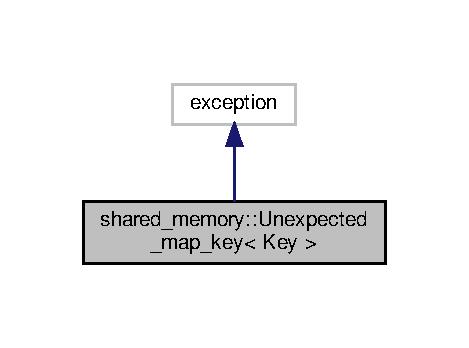
\includegraphics[width=225pt]{classshared__memory_1_1Unexpected__map__key__coll__graph}
\end{center}
\end{figure}
\subsection*{Public Member Functions}
\begin{DoxyCompactItemize}
\item 
\mbox{\Hypertarget{classshared__memory_1_1Unexpected__map__key_a6b186f98c6978fb264529381b3174c9d}\label{classshared__memory_1_1Unexpected__map__key_a6b186f98c6978fb264529381b3174c9d}} 
{\bfseries Unexpected\+\_\+map\+\_\+key} (const std\+::string \&segment\+\_\+id, const std\+::string \&object\+\_\+id, Key \&expected\+\_\+key)
\item 
\mbox{\Hypertarget{classshared__memory_1_1Unexpected__map__key_a6c33648c021589f76d33f75b3cef9550}\label{classshared__memory_1_1Unexpected__map__key_a6c33648c021589f76d33f75b3cef9550}} 
const char $\ast$ {\bfseries what} () const  throw ()
\end{DoxyCompactItemize}
\subsection*{Private Attributes}
\begin{DoxyCompactItemize}
\item 
\mbox{\Hypertarget{classshared__memory_1_1Unexpected__map__key_a67c2b43bc3b41b5584c7fba92acac5cc}\label{classshared__memory_1_1Unexpected__map__key_a67c2b43bc3b41b5584c7fba92acac5cc}} 
std\+::string {\bfseries error\+\_\+message\+\_\+}
\end{DoxyCompactItemize}


The documentation for this class was generated from the following file\+:\begin{DoxyCompactItemize}
\item 
include/shared\+\_\+memory/\hyperlink{exceptions_8h}{exceptions.\+h}\end{DoxyCompactItemize}

\hypertarget{classshared__memory_1_1Unexpected__size__exception}{}\section{shared\+\_\+memory\+:\+:Unexpected\+\_\+size\+\_\+exception Class Reference}
\label{classshared__memory_1_1Unexpected__size__exception}\index{shared\+\_\+memory\+::\+Unexpected\+\_\+size\+\_\+exception@{shared\+\_\+memory\+::\+Unexpected\+\_\+size\+\_\+exception}}


Inheritance diagram for shared\+\_\+memory\+:\+:Unexpected\+\_\+size\+\_\+exception\+:
\nopagebreak
\begin{figure}[H]
\begin{center}
\leavevmode
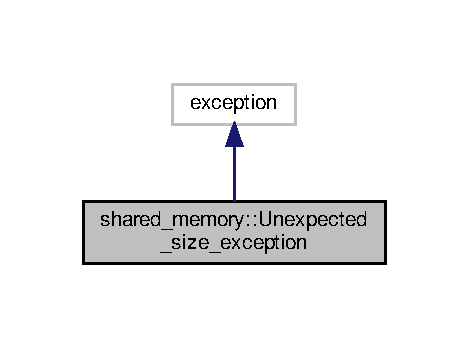
\includegraphics[width=225pt]{classshared__memory_1_1Unexpected__size__exception__inherit__graph}
\end{center}
\end{figure}


Collaboration diagram for shared\+\_\+memory\+:\+:Unexpected\+\_\+size\+\_\+exception\+:
\nopagebreak
\begin{figure}[H]
\begin{center}
\leavevmode
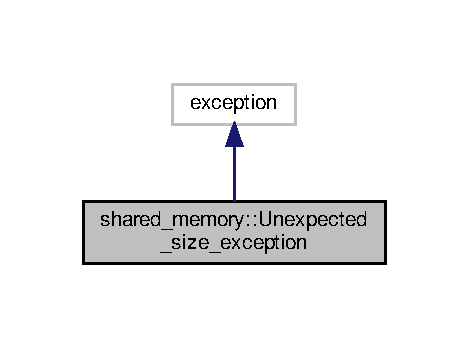
\includegraphics[width=225pt]{classshared__memory_1_1Unexpected__size__exception__coll__graph}
\end{center}
\end{figure}
\subsection*{Public Member Functions}
\begin{DoxyCompactItemize}
\item 
\mbox{\Hypertarget{classshared__memory_1_1Unexpected__size__exception_acc8b3dc1f6879b44e7ccd7f22d13198b}\label{classshared__memory_1_1Unexpected__size__exception_acc8b3dc1f6879b44e7ccd7f22d13198b}} 
{\bfseries Unexpected\+\_\+size\+\_\+exception} (const std\+::string \&segment\+\_\+id, const std\+::string \&object\+\_\+id, int expected\+\_\+size, int size\+\_\+given)
\item 
\mbox{\Hypertarget{classshared__memory_1_1Unexpected__size__exception_a020206032708aad4ad2baa6de11925ac}\label{classshared__memory_1_1Unexpected__size__exception_a020206032708aad4ad2baa6de11925ac}} 
const char $\ast$ {\bfseries what} () const  throw ()
\end{DoxyCompactItemize}
\subsection*{Private Attributes}
\begin{DoxyCompactItemize}
\item 
\mbox{\Hypertarget{classshared__memory_1_1Unexpected__size__exception_a6f22d0e0207e97cafe4f78192c913c55}\label{classshared__memory_1_1Unexpected__size__exception_a6f22d0e0207e97cafe4f78192c913c55}} 
std\+::string {\bfseries error\+\_\+message\+\_\+}
\end{DoxyCompactItemize}


The documentation for this class was generated from the following files\+:\begin{DoxyCompactItemize}
\item 
include/shared\+\_\+memory/\hyperlink{exceptions_8h}{exceptions.\+h}\item 
src/\hyperlink{exceptions_8cpp}{exceptions.\+cpp}\end{DoxyCompactItemize}

\chapter{File Documentation}
\hypertarget{clean__shared__memory_8cpp}{}\section{benchmarks/clean\+\_\+shared\+\_\+memory.cpp File Reference}
\label{clean__shared__memory_8cpp}\index{benchmarks/clean\+\_\+shared\+\_\+memory.\+cpp@{benchmarks/clean\+\_\+shared\+\_\+memory.\+cpp}}


Clean the shared memory of the benchmark, the unnittests, ...  


{\ttfamily \#include $<$boost/interprocess/managed\+\_\+shared\+\_\+memory.\+hpp$>$}\newline
{\ttfamily \#include $<$boost/interprocess/sync/named\+\_\+mutex.\+hpp$>$}\newline
{\ttfamily \#include \char`\"{}shared\+\_\+memory/benchmarks/benchmark\+\_\+common.\+hh\char`\"{}}\newline
Include dependency graph for clean\+\_\+shared\+\_\+memory.\+cpp\+:
\nopagebreak
\begin{figure}[H]
\begin{center}
\leavevmode
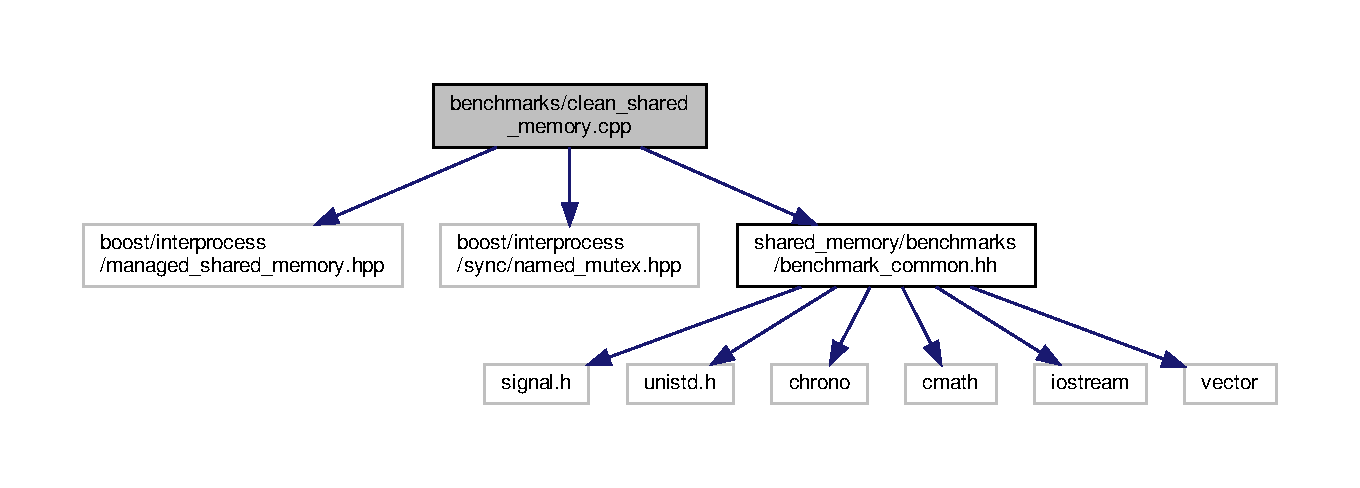
\includegraphics[width=350pt]{clean__shared__memory_8cpp__incl}
\end{center}
\end{figure}
\subsection*{Functions}
\begin{DoxyCompactItemize}
\item 
\mbox{\Hypertarget{clean__shared__memory_8cpp_ae66f6b31b5ad750f1fe042a706a4e3d4}\label{clean__shared__memory_8cpp_ae66f6b31b5ad750f1fe042a706a4e3d4}} 
int {\bfseries main} ()
\end{DoxyCompactItemize}


\subsection{Detailed Description}
Clean the shared memory of the benchmark, the unnittests, ... 

\begin{DoxyAuthor}{Author}
Vincent Berenz 
\end{DoxyAuthor}
\begin{DoxyRefDesc}{License}
\item[\hyperlink{license__license000001}{License}]License B\+S\+D-\/3-\/\+Clause \end{DoxyRefDesc}
\begin{DoxyCopyright}{Copyright}
Copyright (c) 2019, New York University and Max Planck Gesellschaft. 
\end{DoxyCopyright}
\begin{DoxyDate}{Date}
2019-\/05-\/22 
\end{DoxyDate}

\hypertarget{main_8cpp}{}\section{benchmarks/main.cpp File Reference}
\label{main_8cpp}\index{benchmarks/main.\+cpp@{benchmarks/main.\+cpp}}


Initialize and run unittest using the google suit.  


{\ttfamily \#include \char`\"{}gtest/gtest.\+h\char`\"{}}\newline
Include dependency graph for main.\+cpp\+:
\nopagebreak
\begin{figure}[H]
\begin{center}
\leavevmode
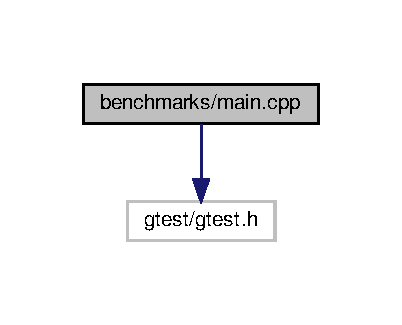
\includegraphics[width=193pt]{main_8cpp__incl}
\end{center}
\end{figure}
\subsection*{Functions}
\begin{DoxyCompactItemize}
\item 
\mbox{\Hypertarget{main_8cpp_a3c04138a5bfe5d72780bb7e82a18e627}\label{main_8cpp_a3c04138a5bfe5d72780bb7e82a18e627}} 
int {\bfseries main} (int argc, char $\ast$$\ast$argv)
\end{DoxyCompactItemize}


\subsection{Detailed Description}
Initialize and run unittest using the google suit. 

\begin{DoxyAuthor}{Author}
Vincent Berenz 
\end{DoxyAuthor}
\begin{DoxyRefDesc}{License}
\item[\hyperlink{license__license000002}{License}]License B\+S\+D-\/3-\/\+Clause \end{DoxyRefDesc}
\begin{DoxyCopyright}{Copyright}
Copyright (c) 2019, New York University and Max Planck Gesellschaft. 
\end{DoxyCopyright}
\begin{DoxyDate}{Date}
2019-\/05-\/22 
\end{DoxyDate}

\hypertarget{stress__get__api_8cpp}{}\section{benchmarks/stress\+\_\+get\+\_\+api.cpp File Reference}
\label{stress__get__api_8cpp}\index{benchmarks/stress\+\_\+get\+\_\+api.\+cpp@{benchmarks/stress\+\_\+get\+\_\+api.\+cpp}}


Benchmark on the get method of the A\+PI.  


{\ttfamily \#include $<$shared\+\_\+memory/benchmarks/benchmark\+\_\+common.\+hh$>$}\newline
{\ttfamily \#include \char`\"{}shared\+\_\+memory/shared\+\_\+memory.\+hpp\char`\"{}}\newline
Include dependency graph for stress\+\_\+get\+\_\+api.\+cpp\+:
\nopagebreak
\begin{figure}[H]
\begin{center}
\leavevmode
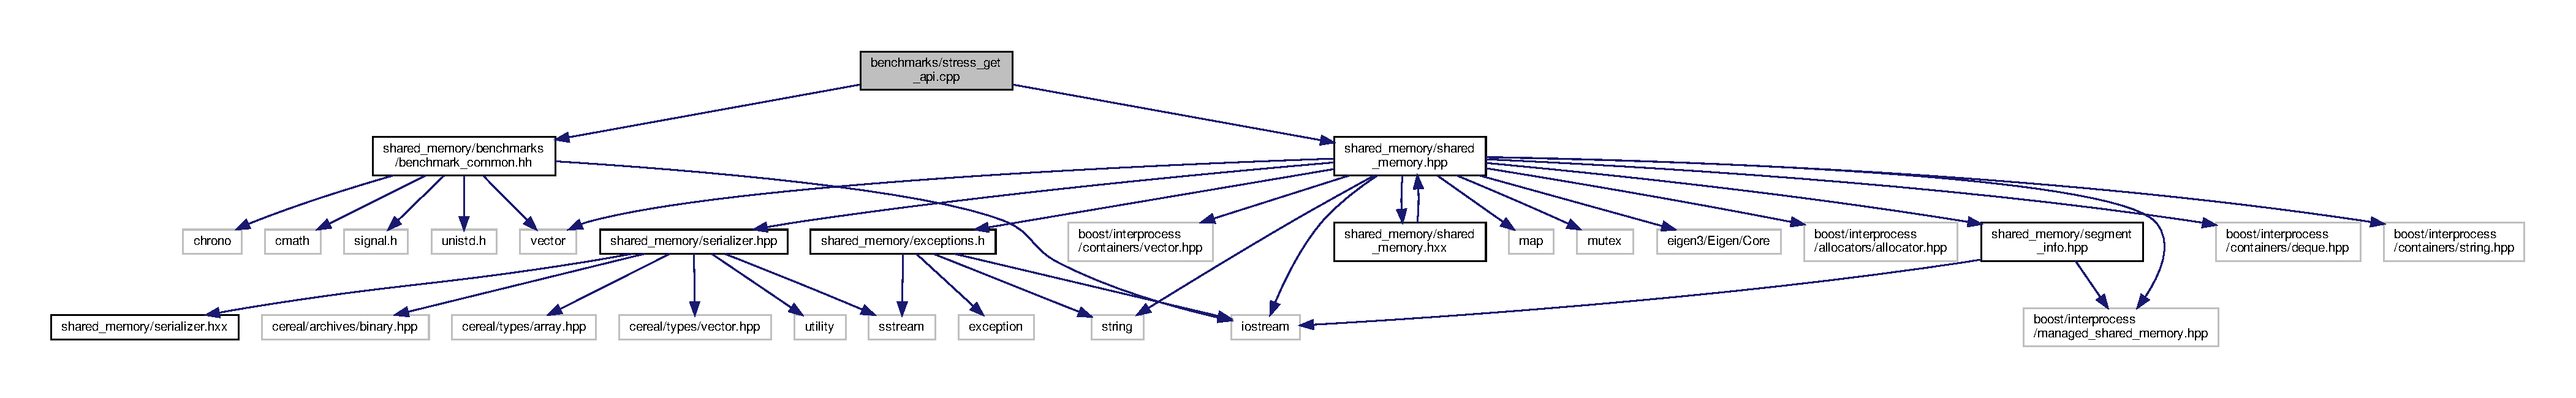
\includegraphics[width=350pt]{stress__get__api_8cpp__incl}
\end{center}
\end{figure}
\subsection*{Functions}
\begin{DoxyCompactItemize}
\item 
\mbox{\Hypertarget{stress__get__api_8cpp_a5d2be5fb88fef648640fe973785d58b1}\label{stress__get__api_8cpp_a5d2be5fb88fef648640fe973785d58b1}} 
void {\bfseries cleaning\+\_\+memory} (int)
\item 
\mbox{\Hypertarget{stress__get__api_8cpp_ae66f6b31b5ad750f1fe042a706a4e3d4}\label{stress__get__api_8cpp_ae66f6b31b5ad750f1fe042a706a4e3d4}} 
int {\bfseries main} ()
\end{DoxyCompactItemize}


\subsection{Detailed Description}
Benchmark on the get method of the A\+PI. 

\begin{DoxyAuthor}{Author}
Vincent Berenz 
\end{DoxyAuthor}
\begin{DoxyRefDesc}{License}
\item[\hyperlink{license__license000003}{License}]License B\+S\+D-\/3-\/\+Clause \end{DoxyRefDesc}
\begin{DoxyCopyright}{Copyright}
Copyright (c) 2019, New York University and Max Planck Gesellschaft. 
\end{DoxyCopyright}
\begin{DoxyDate}{Date}
2019-\/05-\/22 
\end{DoxyDate}

\hypertarget{stress__get__raw__boost__efficient_8cpp}{}\section{benchmarks/stress\+\_\+get\+\_\+raw\+\_\+boost\+\_\+efficient.cpp File Reference}
\label{stress__get__raw__boost__efficient_8cpp}\index{benchmarks/stress\+\_\+get\+\_\+raw\+\_\+boost\+\_\+efficient.\+cpp@{benchmarks/stress\+\_\+get\+\_\+raw\+\_\+boost\+\_\+efficient.\+cpp}}


Use the raw boost A\+PI in order to compare the efficiency of the new A\+PI compare to the standard boost A\+PI.  


{\ttfamily \#include $<$boost/interprocess/managed\+\_\+shared\+\_\+memory.\+hpp$>$}\\*
{\ttfamily \#include $<$boost/interprocess/sync/named\+\_\+mutex.\+hpp$>$}\\*
{\ttfamily \#include \char`\"{}shared\+\_\+memory/benchmarks/benchmark\+\_\+common.\+hh\char`\"{}}\\*
Include dependency graph for stress\+\_\+get\+\_\+raw\+\_\+boost\+\_\+efficient.\+cpp\+:
\nopagebreak
\begin{figure}[H]
\begin{center}
\leavevmode
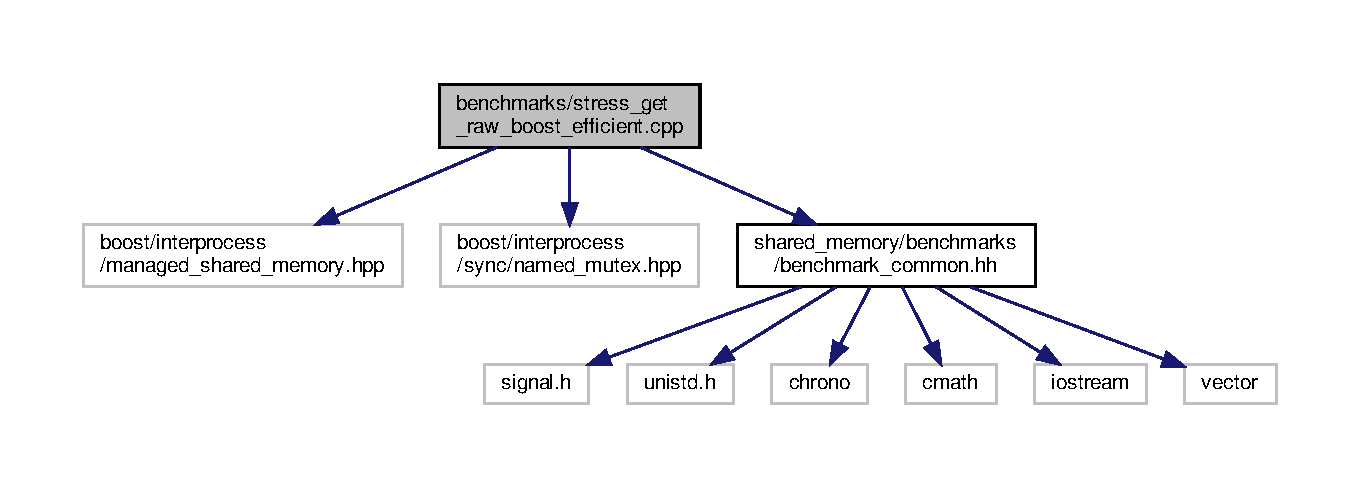
\includegraphics[width=350pt]{stress__get__raw__boost__efficient_8cpp__incl}
\end{center}
\end{figure}
\subsection*{Functions}
\begin{DoxyCompactItemize}
\item 
void {\bfseries cleaning\+\_\+memory} (int)\hypertarget{stress__get__raw__boost__efficient_8cpp_a5d2be5fb88fef648640fe973785d58b1}{}\label{stress__get__raw__boost__efficient_8cpp_a5d2be5fb88fef648640fe973785d58b1}

\item 
int {\bfseries main} ()\hypertarget{stress__get__raw__boost__efficient_8cpp_ae66f6b31b5ad750f1fe042a706a4e3d4}{}\label{stress__get__raw__boost__efficient_8cpp_ae66f6b31b5ad750f1fe042a706a4e3d4}

\end{DoxyCompactItemize}


\subsection{Detailed Description}
Use the raw boost A\+PI in order to compare the efficiency of the new A\+PI compare to the standard boost A\+PI. 

\begin{DoxyAuthor}{Author}
Vincent Berenz 
\end{DoxyAuthor}
\begin{DoxyRefDesc}{License}
\item[\hyperlink{license__license000004}{License}]License B\+S\+D-\/3-\/\+Clause \end{DoxyRefDesc}
\begin{DoxyCopyright}{Copyright}
Copyright (c) 2019, New York University and Max Planck Gesellschaft. 
\end{DoxyCopyright}
\begin{DoxyDate}{Date}
2019-\/05-\/22 
\end{DoxyDate}

\hypertarget{stress__get__raw__boost__inefficient_8cpp}{}\section{benchmarks/stress\+\_\+get\+\_\+raw\+\_\+boost\+\_\+inefficient.cpp File Reference}
\label{stress__get__raw__boost__inefficient_8cpp}\index{benchmarks/stress\+\_\+get\+\_\+raw\+\_\+boost\+\_\+inefficient.\+cpp@{benchmarks/stress\+\_\+get\+\_\+raw\+\_\+boost\+\_\+inefficient.\+cpp}}


Use the raw boost A\+PI in order to compare the efficiency of the new A\+PI compare to the standard boost A\+PI.  


{\ttfamily \#include $<$boost/interprocess/managed\+\_\+shared\+\_\+memory.\+hpp$>$}\newline
{\ttfamily \#include $<$boost/interprocess/sync/named\+\_\+mutex.\+hpp$>$}\newline
{\ttfamily \#include \char`\"{}shared\+\_\+memory/benchmarks/benchmark\+\_\+common.\+hh\char`\"{}}\newline
Include dependency graph for stress\+\_\+get\+\_\+raw\+\_\+boost\+\_\+inefficient.\+cpp\+:
\nopagebreak
\begin{figure}[H]
\begin{center}
\leavevmode
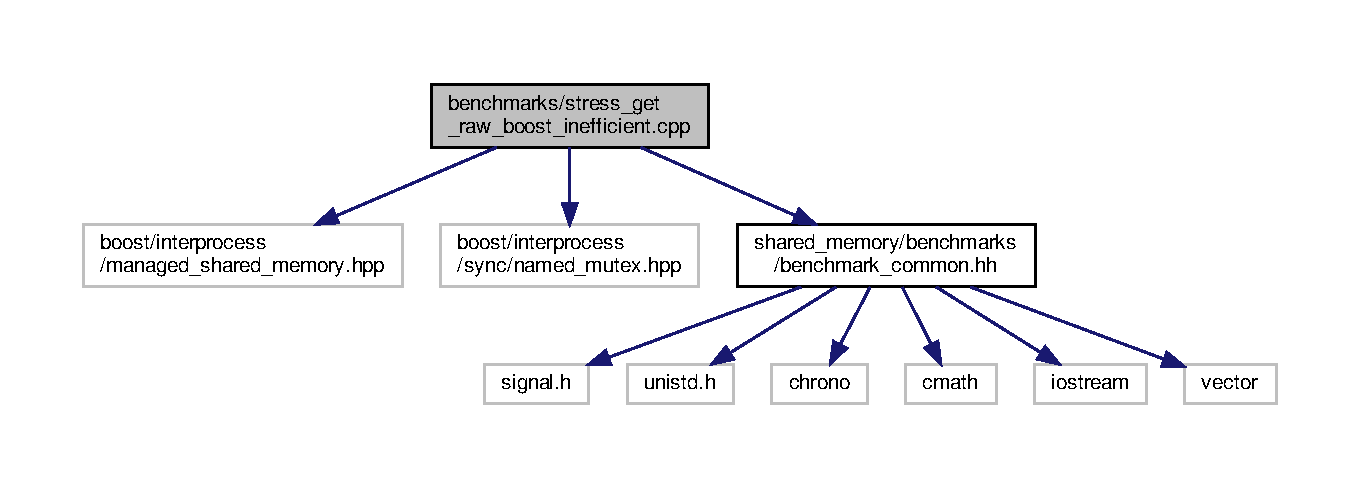
\includegraphics[width=350pt]{stress__get__raw__boost__inefficient_8cpp__incl}
\end{center}
\end{figure}
\subsection*{Functions}
\begin{DoxyCompactItemize}
\item 
\mbox{\Hypertarget{stress__get__raw__boost__inefficient_8cpp_a5d2be5fb88fef648640fe973785d58b1}\label{stress__get__raw__boost__inefficient_8cpp_a5d2be5fb88fef648640fe973785d58b1}} 
void {\bfseries cleaning\+\_\+memory} (int)
\item 
\mbox{\Hypertarget{stress__get__raw__boost__inefficient_8cpp_ae66f6b31b5ad750f1fe042a706a4e3d4}\label{stress__get__raw__boost__inefficient_8cpp_ae66f6b31b5ad750f1fe042a706a4e3d4}} 
int {\bfseries main} ()
\end{DoxyCompactItemize}


\subsection{Detailed Description}
Use the raw boost A\+PI in order to compare the efficiency of the new A\+PI compare to the standard boost A\+PI. 

\begin{DoxyAuthor}{Author}
Vincent Berenz 
\end{DoxyAuthor}
\begin{DoxyRefDesc}{License}
\item[\hyperlink{license__license000005}{License}]License B\+S\+D-\/3-\/\+Clause \end{DoxyRefDesc}
\begin{DoxyCopyright}{Copyright}
Copyright (c) 2019, New York University and Max Planck Gesellschaft. 
\end{DoxyCopyright}
\begin{DoxyDate}{Date}
2019-\/05-\/22 
\end{DoxyDate}

\hypertarget{stress__set__api_8cpp}{}\section{benchmarks/stress\+\_\+set\+\_\+api.cpp File Reference}
\label{stress__set__api_8cpp}\index{benchmarks/stress\+\_\+set\+\_\+api.\+cpp@{benchmarks/stress\+\_\+set\+\_\+api.\+cpp}}


Benchmark the set method form the A\+PI.  


{\ttfamily \#include \char`\"{}shared\+\_\+memory/benchmarks/benchmark\+\_\+common.\+hh\char`\"{}}\\*
{\ttfamily \#include \char`\"{}shared\+\_\+memory/shared\+\_\+memory.\+hpp\char`\"{}}\\*
Include dependency graph for stress\+\_\+set\+\_\+api.\+cpp\+:
\nopagebreak
\begin{figure}[H]
\begin{center}
\leavevmode
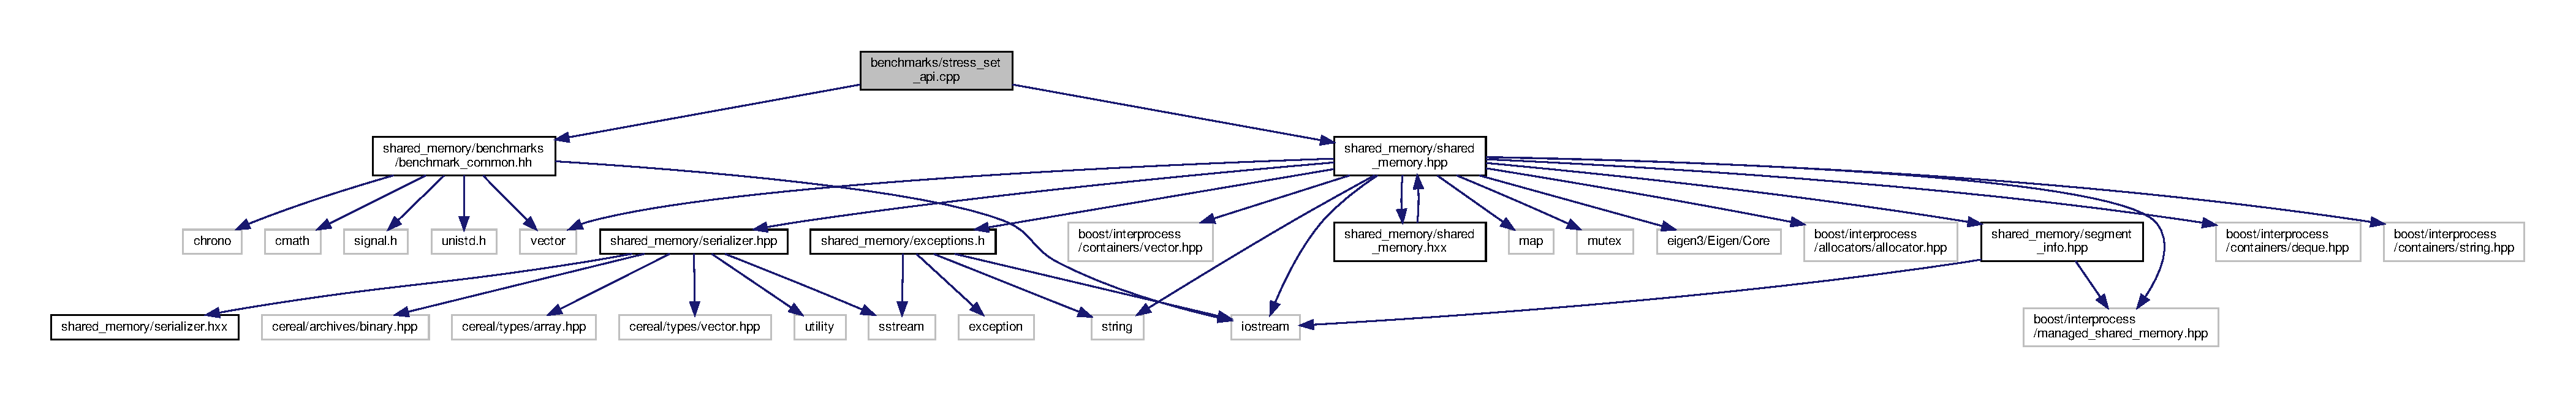
\includegraphics[width=350pt]{stress__set__api_8cpp__incl}
\end{center}
\end{figure}
\subsection*{Functions}
\begin{DoxyCompactItemize}
\item 
void {\bfseries cleaning\+\_\+memory} (int)\hypertarget{stress__set__api_8cpp_a5d2be5fb88fef648640fe973785d58b1}{}\label{stress__set__api_8cpp_a5d2be5fb88fef648640fe973785d58b1}

\item 
int {\bfseries main} ()\hypertarget{stress__set__api_8cpp_ae66f6b31b5ad750f1fe042a706a4e3d4}{}\label{stress__set__api_8cpp_ae66f6b31b5ad750f1fe042a706a4e3d4}

\end{DoxyCompactItemize}


\subsection{Detailed Description}
Benchmark the set method form the A\+PI. 

\begin{DoxyAuthor}{Author}
Vincent Berenz 
\end{DoxyAuthor}
\begin{DoxyRefDesc}{License}
\item[\hyperlink{license__license000006}{License}]License B\+S\+D-\/3-\/\+Clause \end{DoxyRefDesc}
\begin{DoxyCopyright}{Copyright}
Copyright (c) 2019, New York University and Max Planck Gesellschaft. 
\end{DoxyCopyright}
\begin{DoxyDate}{Date}
2019-\/05-\/22 
\end{DoxyDate}

\hypertarget{stress__set__raw__boost__efficient_8cpp}{}\section{benchmarks/stress\+\_\+set\+\_\+raw\+\_\+boost\+\_\+efficient.cpp File Reference}
\label{stress__set__raw__boost__efficient_8cpp}\index{benchmarks/stress\+\_\+set\+\_\+raw\+\_\+boost\+\_\+efficient.\+cpp@{benchmarks/stress\+\_\+set\+\_\+raw\+\_\+boost\+\_\+efficient.\+cpp}}


Use the raw boost A\+PI in order to compare the efficiency of the new A\+PI compare to the standard boost A\+PI.  


{\ttfamily \#include $<$boost/interprocess/managed\+\_\+shared\+\_\+memory.\+hpp$>$}\newline
{\ttfamily \#include $<$boost/interprocess/sync/named\+\_\+mutex.\+hpp$>$}\newline
{\ttfamily \#include \char`\"{}shared\+\_\+memory/benchmarks/benchmark\+\_\+common.\+hh\char`\"{}}\newline
Include dependency graph for stress\+\_\+set\+\_\+raw\+\_\+boost\+\_\+efficient.\+cpp\+:
\nopagebreak
\begin{figure}[H]
\begin{center}
\leavevmode
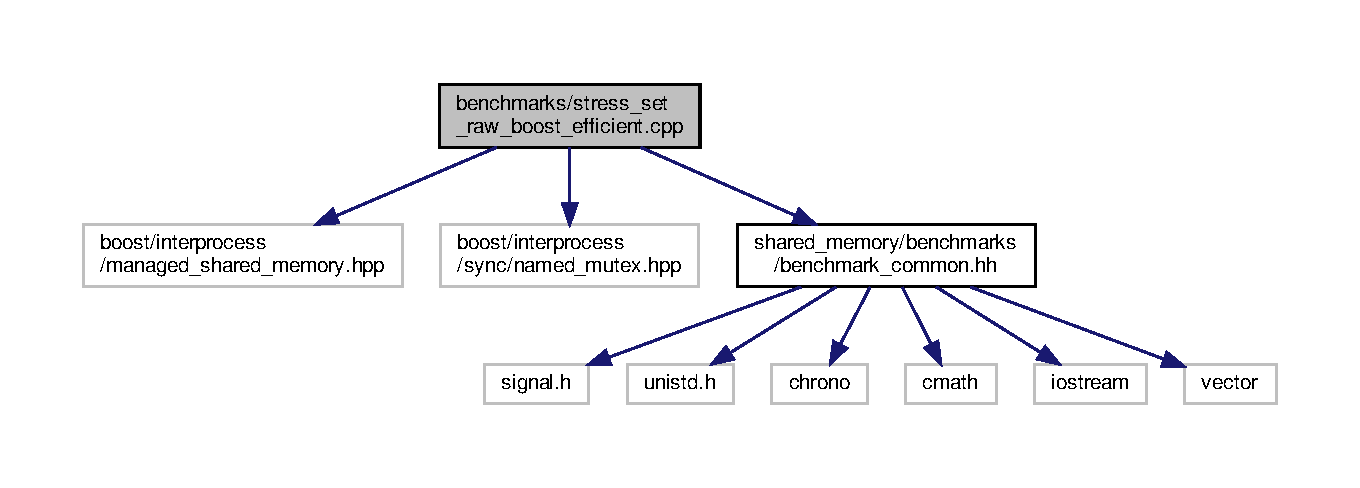
\includegraphics[width=350pt]{stress__set__raw__boost__efficient_8cpp__incl}
\end{center}
\end{figure}
\subsection*{Functions}
\begin{DoxyCompactItemize}
\item 
\mbox{\Hypertarget{stress__set__raw__boost__efficient_8cpp_a5d2be5fb88fef648640fe973785d58b1}\label{stress__set__raw__boost__efficient_8cpp_a5d2be5fb88fef648640fe973785d58b1}} 
void {\bfseries cleaning\+\_\+memory} (int)
\item 
\mbox{\Hypertarget{stress__set__raw__boost__efficient_8cpp_ae66f6b31b5ad750f1fe042a706a4e3d4}\label{stress__set__raw__boost__efficient_8cpp_ae66f6b31b5ad750f1fe042a706a4e3d4}} 
int {\bfseries main} ()
\end{DoxyCompactItemize}


\subsection{Detailed Description}
Use the raw boost A\+PI in order to compare the efficiency of the new A\+PI compare to the standard boost A\+PI. 

\begin{DoxyAuthor}{Author}
Vincent Berenz 
\end{DoxyAuthor}
\begin{DoxyRefDesc}{License}
\item[\hyperlink{license__license000007}{License}]License B\+S\+D-\/3-\/\+Clause \end{DoxyRefDesc}
\begin{DoxyCopyright}{Copyright}
Copyright (c) 2019, New York University and Max Planck Gesellschaft. 
\end{DoxyCopyright}
\begin{DoxyDate}{Date}
2019-\/05-\/22 
\end{DoxyDate}

\hypertarget{stress__set__raw__boost__inefficient_8cpp}{}\section{benchmarks/stress\+\_\+set\+\_\+raw\+\_\+boost\+\_\+inefficient.cpp File Reference}
\label{stress__set__raw__boost__inefficient_8cpp}\index{benchmarks/stress\+\_\+set\+\_\+raw\+\_\+boost\+\_\+inefficient.\+cpp@{benchmarks/stress\+\_\+set\+\_\+raw\+\_\+boost\+\_\+inefficient.\+cpp}}


Use the raw boost A\+PI in order to compare the efficiency of the new A\+PI compare to the standard boost A\+PI.  


{\ttfamily \#include $<$boost/interprocess/managed\+\_\+shared\+\_\+memory.\+hpp$>$}\newline
{\ttfamily \#include $<$boost/interprocess/sync/named\+\_\+mutex.\+hpp$>$}\newline
{\ttfamily \#include \char`\"{}shared\+\_\+memory/benchmarks/benchmark\+\_\+common.\+hh\char`\"{}}\newline
Include dependency graph for stress\+\_\+set\+\_\+raw\+\_\+boost\+\_\+inefficient.\+cpp\+:
\nopagebreak
\begin{figure}[H]
\begin{center}
\leavevmode
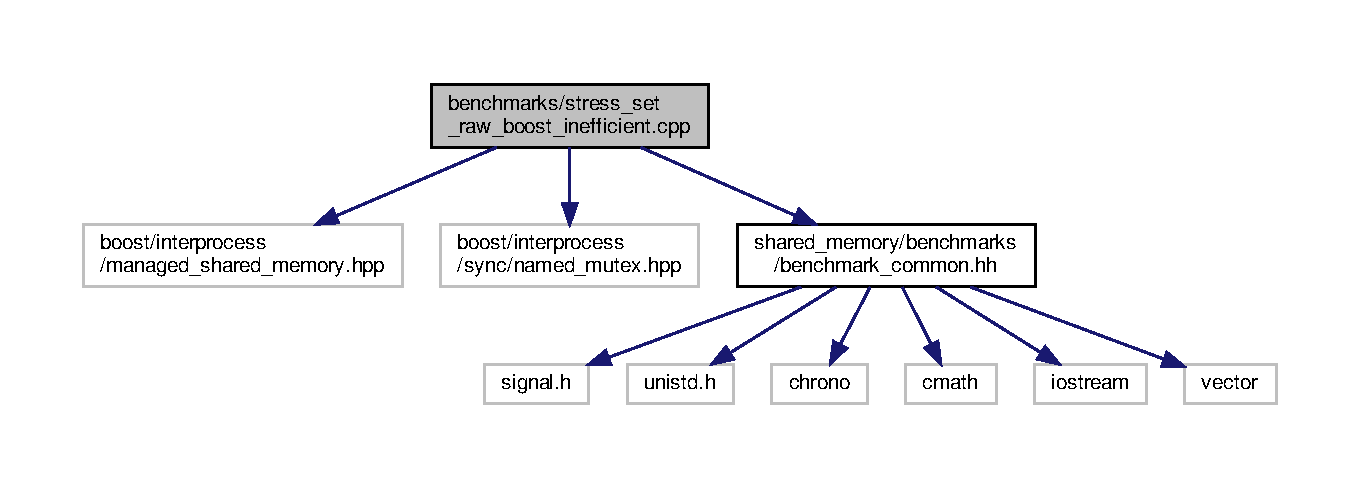
\includegraphics[width=350pt]{stress__set__raw__boost__inefficient_8cpp__incl}
\end{center}
\end{figure}
\subsection*{Functions}
\begin{DoxyCompactItemize}
\item 
\mbox{\Hypertarget{stress__set__raw__boost__inefficient_8cpp_a5d2be5fb88fef648640fe973785d58b1}\label{stress__set__raw__boost__inefficient_8cpp_a5d2be5fb88fef648640fe973785d58b1}} 
void {\bfseries cleaning\+\_\+memory} (int)
\item 
\mbox{\Hypertarget{stress__set__raw__boost__inefficient_8cpp_ae66f6b31b5ad750f1fe042a706a4e3d4}\label{stress__set__raw__boost__inefficient_8cpp_ae66f6b31b5ad750f1fe042a706a4e3d4}} 
int {\bfseries main} ()
\end{DoxyCompactItemize}


\subsection{Detailed Description}
Use the raw boost A\+PI in order to compare the efficiency of the new A\+PI compare to the standard boost A\+PI. 

\begin{DoxyAuthor}{Author}
Vincent Berenz 
\end{DoxyAuthor}
\begin{DoxyRefDesc}{License}
\item[\hyperlink{license__license000008}{License}]License B\+S\+D-\/3-\/\+Clause \end{DoxyRefDesc}
\begin{DoxyCopyright}{Copyright}
Copyright (c) 2019, New York University and Max Planck Gesellschaft. 
\end{DoxyCopyright}
\begin{DoxyDate}{Date}
2019-\/05-\/22 
\end{DoxyDate}

\hypertarget{demo__read__array_8cpp}{}\section{demos/demo\+\_\+read\+\_\+array.cpp File Reference}
\label{demo__read__array_8cpp}\index{demos/demo\+\_\+read\+\_\+array.\+cpp@{demos/demo\+\_\+read\+\_\+array.\+cpp}}


example of reading from interprocesses arrays  


{\ttfamily \#include $<$signal.\+h$>$}\newline
{\ttfamily \#include $<$unistd.\+h$>$}\newline
{\ttfamily \#include \char`\"{}shared\+\_\+memory/array.\+hpp\char`\"{}}\newline
{\ttfamily \#include \char`\"{}shared\+\_\+memory/demos/item.\+hpp\char`\"{}}\newline
Include dependency graph for demo\+\_\+read\+\_\+array.\+cpp\+:
\nopagebreak
\begin{figure}[H]
\begin{center}
\leavevmode
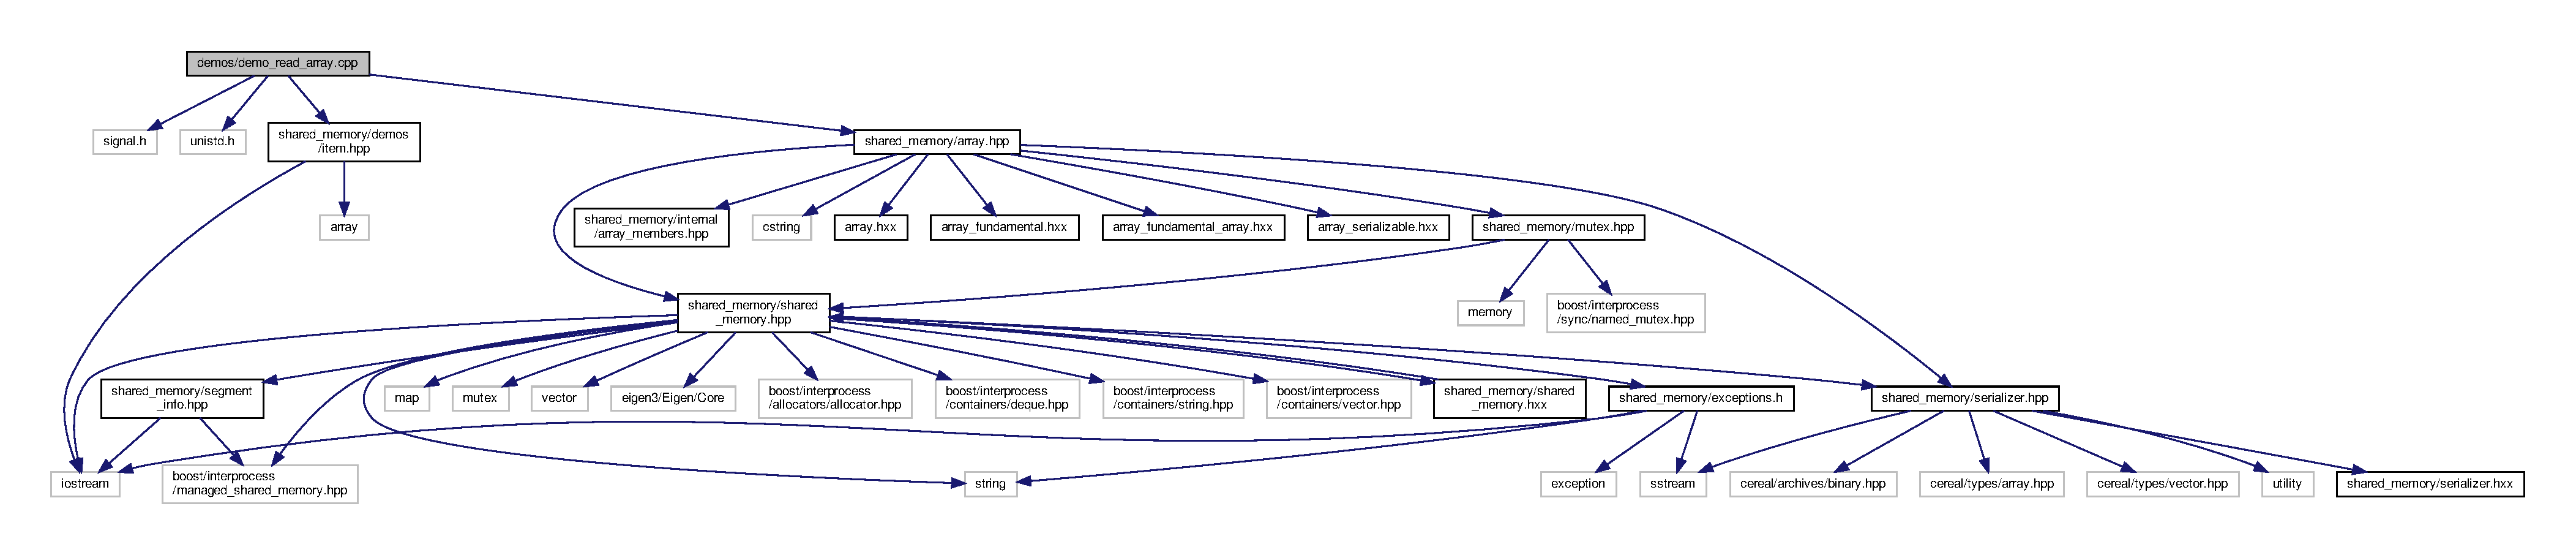
\includegraphics[width=350pt]{demo__read__array_8cpp__incl}
\end{center}
\end{figure}
\subsection*{Macros}
\begin{DoxyCompactItemize}
\item 
\mbox{\Hypertarget{demo__read__array_8cpp_a70ed59adcb4159ac551058053e649640}\label{demo__read__array_8cpp_a70ed59adcb4159ac551058053e649640}} 
\#define {\bfseries S\+I\+ZE}~4
\item 
\mbox{\Hypertarget{demo__read__array_8cpp_a715f5eb54a3e370e08f6eacb579cb462}\label{demo__read__array_8cpp_a715f5eb54a3e370e08f6eacb579cb462}} 
\#define {\bfseries S\+E\+G\+M\+E\+N\+T\+\_\+\+S\+E\+R\+I\+A\+L\+I\+Z\+ED}~\char`\"{}demo\+\_\+array\+\_\+serialized\char`\"{}
\item 
\mbox{\Hypertarget{demo__read__array_8cpp_a56db1002f1652200987b0a138c59516b}\label{demo__read__array_8cpp_a56db1002f1652200987b0a138c59516b}} 
\#define {\bfseries S\+E\+G\+M\+E\+N\+T\+\_\+\+F\+U\+N\+D\+A\+M\+E\+N\+T\+AL}~\char`\"{}demo\+\_\+array\+\_\+fundamental\char`\"{}
\item 
\mbox{\Hypertarget{demo__read__array_8cpp_ac053d74fd470967d07823e1e5aa3137a}\label{demo__read__array_8cpp_ac053d74fd470967d07823e1e5aa3137a}} 
\#define {\bfseries S\+E\+G\+M\+E\+N\+T\+\_\+\+F\+U\+N\+D\+A\+M\+E\+N\+T\+A\+L\+\_\+\+A\+R\+R\+AY}~\char`\"{}demo\+\_\+array\+\_\+fundamental\+\_\+array\char`\"{}
\end{DoxyCompactItemize}
\subsection*{Functions}
\begin{DoxyCompactItemize}
\item 
\mbox{\Hypertarget{demo__read__array_8cpp_aba399b0a6a6e3bd37af95bd04e8def6f}\label{demo__read__array_8cpp_aba399b0a6a6e3bd37af95bd04e8def6f}} 
void {\bfseries stop} (int)
\item 
\mbox{\Hypertarget{demo__read__array_8cpp_aaccf071805315d6cb393abaa3d052435}\label{demo__read__array_8cpp_aaccf071805315d6cb393abaa3d052435}} 
void {\bfseries print\+\_\+array} (int $\ast$values, int size)
\item 
\mbox{\Hypertarget{demo__read__array_8cpp_a13a43e6d814de94978c515cb084873b1}\label{demo__read__array_8cpp_a13a43e6d814de94978c515cb084873b1}} 
void \hyperlink{demo__read__array_8cpp_a13a43e6d814de94978c515cb084873b1}{run} ()
\begin{DoxyCompactList}\small\item\em read from the array created by demo\+\_\+write\+\_\+array, which should have been started before this demo was (infinite hanging expected otherwise) \end{DoxyCompactList}\item 
\mbox{\Hypertarget{demo__read__array_8cpp_ae66f6b31b5ad750f1fe042a706a4e3d4}\label{demo__read__array_8cpp_ae66f6b31b5ad750f1fe042a706a4e3d4}} 
int {\bfseries main} ()
\end{DoxyCompactItemize}
\subsection*{Variables}
\begin{DoxyCompactItemize}
\item 
\mbox{\Hypertarget{demo__read__array_8cpp_a383e703fc3e9dd425f075cf463ee4c5b}\label{demo__read__array_8cpp_a383e703fc3e9dd425f075cf463ee4c5b}} 
static bool {\bfseries R\+U\+N\+N\+I\+NG} = true
\end{DoxyCompactItemize}


\subsection{Detailed Description}
example of reading from interprocesses arrays 

\begin{DoxyAuthor}{Author}
Vincent Berenz license License B\+S\+D-\/3-\/\+Clause 
\end{DoxyAuthor}
\begin{DoxyCopyright}{Copyright}
Copyright (c) 2019, New York University and Max Planck Gesellshaft. 
\end{DoxyCopyright}
\begin{DoxyDate}{Date}
2019-\/05-\/22 
\end{DoxyDate}

\hypertarget{demo__write__array_8cpp}{}\section{demos/demo\+\_\+write\+\_\+array.cpp File Reference}
\label{demo__write__array_8cpp}\index{demos/demo\+\_\+write\+\_\+array.\+cpp@{demos/demo\+\_\+write\+\_\+array.\+cpp}}


example of writing into interprocesses arrays  


{\ttfamily \#include $<$signal.\+h$>$}\newline
{\ttfamily \#include $<$unistd.\+h$>$}\newline
{\ttfamily \#include \char`\"{}shared\+\_\+memory/array.\+hpp\char`\"{}}\newline
{\ttfamily \#include \char`\"{}shared\+\_\+memory/demos/item.\+hpp\char`\"{}}\newline
Include dependency graph for demo\+\_\+write\+\_\+array.\+cpp\+:
\nopagebreak
\begin{figure}[H]
\begin{center}
\leavevmode
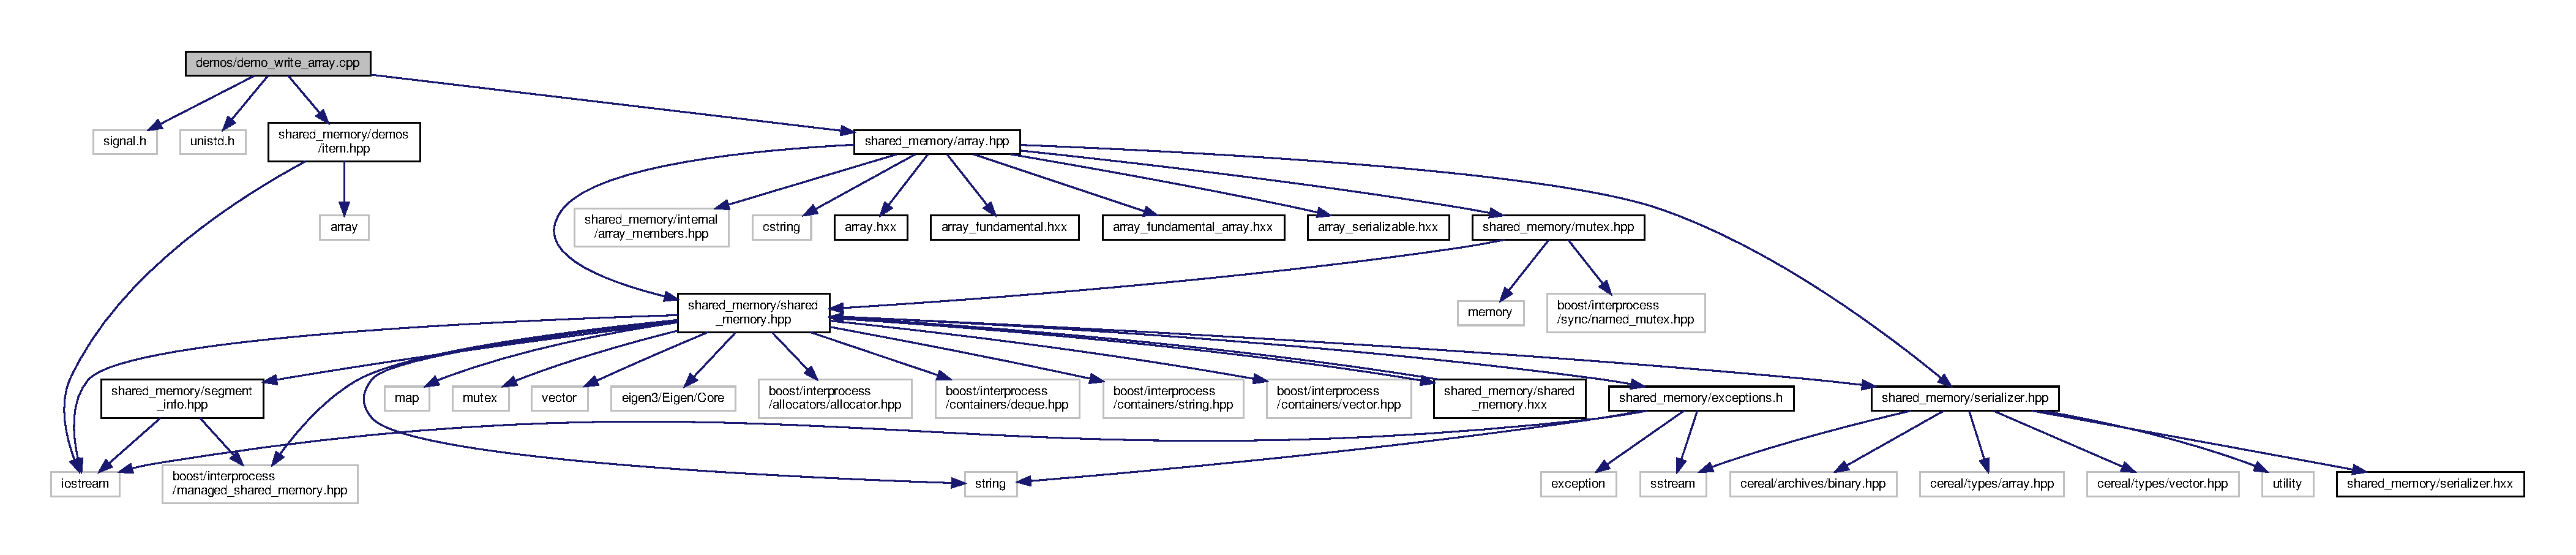
\includegraphics[width=350pt]{demo__write__array_8cpp__incl}
\end{center}
\end{figure}
\subsection*{Macros}
\begin{DoxyCompactItemize}
\item 
\mbox{\Hypertarget{demo__write__array_8cpp_a70ed59adcb4159ac551058053e649640}\label{demo__write__array_8cpp_a70ed59adcb4159ac551058053e649640}} 
\#define {\bfseries S\+I\+ZE}~4
\item 
\mbox{\Hypertarget{demo__write__array_8cpp_a715f5eb54a3e370e08f6eacb579cb462}\label{demo__write__array_8cpp_a715f5eb54a3e370e08f6eacb579cb462}} 
\#define {\bfseries S\+E\+G\+M\+E\+N\+T\+\_\+\+S\+E\+R\+I\+A\+L\+I\+Z\+ED}~\char`\"{}demo\+\_\+array\+\_\+serialized\char`\"{}
\item 
\mbox{\Hypertarget{demo__write__array_8cpp_a56db1002f1652200987b0a138c59516b}\label{demo__write__array_8cpp_a56db1002f1652200987b0a138c59516b}} 
\#define {\bfseries S\+E\+G\+M\+E\+N\+T\+\_\+\+F\+U\+N\+D\+A\+M\+E\+N\+T\+AL}~\char`\"{}demo\+\_\+array\+\_\+fundamental\char`\"{}
\item 
\mbox{\Hypertarget{demo__write__array_8cpp_ac053d74fd470967d07823e1e5aa3137a}\label{demo__write__array_8cpp_ac053d74fd470967d07823e1e5aa3137a}} 
\#define {\bfseries S\+E\+G\+M\+E\+N\+T\+\_\+\+F\+U\+N\+D\+A\+M\+E\+N\+T\+A\+L\+\_\+\+A\+R\+R\+AY}~\char`\"{}demo\+\_\+array\+\_\+fundamental\+\_\+array\char`\"{}
\end{DoxyCompactItemize}
\subsection*{Functions}
\begin{DoxyCompactItemize}
\item 
\mbox{\Hypertarget{demo__write__array_8cpp_aba399b0a6a6e3bd37af95bd04e8def6f}\label{demo__write__array_8cpp_aba399b0a6a6e3bd37af95bd04e8def6f}} 
void {\bfseries stop} (int)
\item 
void \hyperlink{demo__write__array_8cpp_a13a43e6d814de94978c515cb084873b1}{run} ()
\begin{DoxyCompactList}\small\item\em create interprocesses arrays and write into them. \end{DoxyCompactList}\item 
\mbox{\Hypertarget{demo__write__array_8cpp_ae66f6b31b5ad750f1fe042a706a4e3d4}\label{demo__write__array_8cpp_ae66f6b31b5ad750f1fe042a706a4e3d4}} 
int {\bfseries main} ()
\end{DoxyCompactItemize}
\subsection*{Variables}
\begin{DoxyCompactItemize}
\item 
\mbox{\Hypertarget{demo__write__array_8cpp_a383e703fc3e9dd425f075cf463ee4c5b}\label{demo__write__array_8cpp_a383e703fc3e9dd425f075cf463ee4c5b}} 
static bool {\bfseries R\+U\+N\+N\+I\+NG} = true
\end{DoxyCompactItemize}


\subsection{Detailed Description}
example of writing into interprocesses arrays 

\begin{DoxyAuthor}{Author}
Vincent Berenz license License B\+S\+D-\/3-\/\+Clause 
\end{DoxyAuthor}
\begin{DoxyCopyright}{Copyright}
Copyright (c) 2019, New York University and Max Planck Gesellshaft. 
\end{DoxyCopyright}
\begin{DoxyDate}{Date}
2019-\/05-\/22 
\end{DoxyDate}


\subsection{Function Documentation}
\mbox{\Hypertarget{demo__write__array_8cpp_a13a43e6d814de94978c515cb084873b1}\label{demo__write__array_8cpp_a13a43e6d814de94978c515cb084873b1}} 
\index{demo\+\_\+write\+\_\+array.\+cpp@{demo\+\_\+write\+\_\+array.\+cpp}!run@{run}}
\index{run@{run}!demo\+\_\+write\+\_\+array.\+cpp@{demo\+\_\+write\+\_\+array.\+cpp}}
\subsubsection{\texorpdfstring{run()}{run()}}
{\footnotesize\ttfamily void run (\begin{DoxyParamCaption}{ }\end{DoxyParamCaption})}



create interprocesses arrays and write into them. 

Run demo\+\_\+read\+\_\+array for a process reading these arrays 
\hypertarget{exchange__manager__consumer_8cpp}{}\section{demos/exchange\+\_\+manager\+\_\+consumer.cpp File Reference}
\label{exchange__manager__consumer_8cpp}\index{demos/exchange\+\_\+manager\+\_\+consumer.\+cpp@{demos/exchange\+\_\+manager\+\_\+consumer.\+cpp}}


Demonstrate how to use the exchange manage consummer.  


{\ttfamily \#include \char`\"{}shared\+\_\+memory/exchange\+\_\+manager\+\_\+consumer.\+hpp\char`\"{}}\newline
{\ttfamily \#include $<$signal.\+h$>$}\newline
{\ttfamily \#include $<$stdlib.\+h$>$}\newline
{\ttfamily \#include $<$time.\+h$>$}\newline
{\ttfamily \#include $<$unistd.\+h$>$}\newline
{\ttfamily \#include $<$iostream$>$}\newline
{\ttfamily \#include \char`\"{}shared\+\_\+memory/demos/four\+\_\+int\+\_\+values.\+hpp\char`\"{}}\newline
Include dependency graph for exchange\+\_\+manager\+\_\+consumer.\+cpp\+:
\nopagebreak
\begin{figure}[H]
\begin{center}
\leavevmode
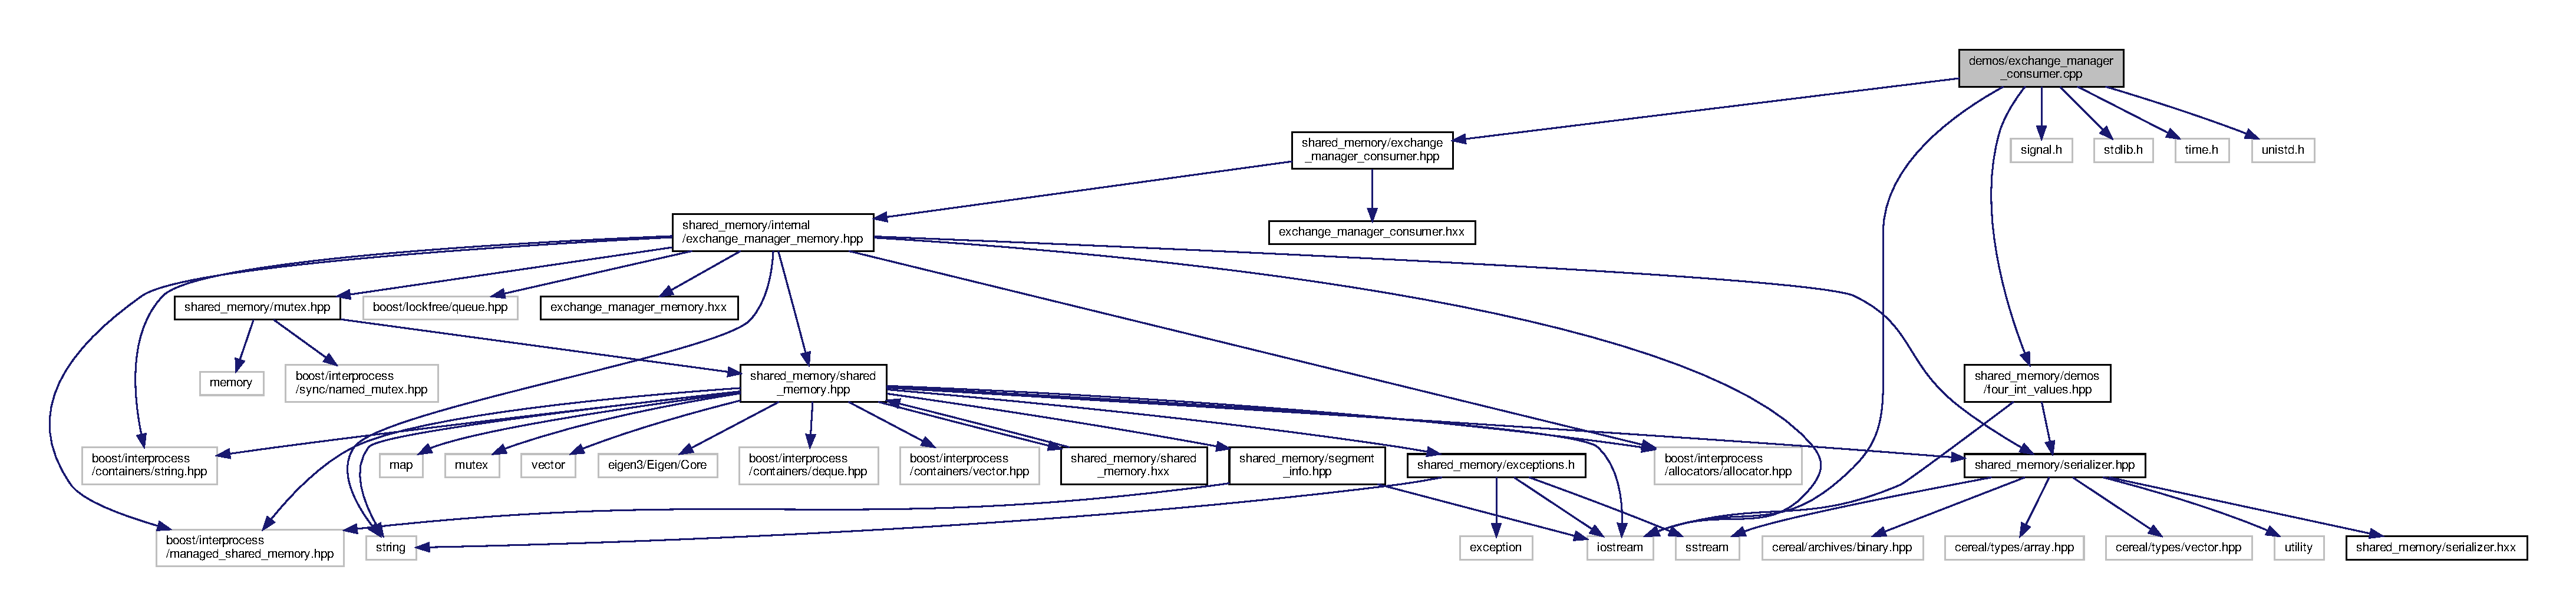
\includegraphics[width=350pt]{exchange__manager__consumer_8cpp__incl}
\end{center}
\end{figure}
\subsection*{Macros}
\begin{DoxyCompactItemize}
\item 
\mbox{\Hypertarget{exchange__manager__consumer_8cpp_aa2341624eba49f3cdec3d9656b97cd79}\label{exchange__manager__consumer_8cpp_aa2341624eba49f3cdec3d9656b97cd79}} 
\#define {\bfseries S\+E\+G\+M\+E\+N\+T\+\_\+\+ID}~\char`\"{}exchange\+\_\+demo\+\_\+segment\char`\"{}
\item 
\mbox{\Hypertarget{exchange__manager__consumer_8cpp_a7996b622059a5fb225b909180b1d385e}\label{exchange__manager__consumer_8cpp_a7996b622059a5fb225b909180b1d385e}} 
\#define {\bfseries O\+B\+J\+E\+C\+T\+\_\+\+ID}~\char`\"{}exchange\+\_\+demo\+\_\+object\char`\"{}
\item 
\mbox{\Hypertarget{exchange__manager__consumer_8cpp_a142810068f1b99cd93d3fc9f0e160e02}\label{exchange__manager__consumer_8cpp_a142810068f1b99cd93d3fc9f0e160e02}} 
\#define {\bfseries Q\+U\+E\+U\+E\+\_\+\+S\+I\+ZE}~2000 $\ast$ 4
\end{DoxyCompactItemize}
\subsection*{Functions}
\begin{DoxyCompactItemize}
\item 
\mbox{\Hypertarget{exchange__manager__consumer_8cpp_aba399b0a6a6e3bd37af95bd04e8def6f}\label{exchange__manager__consumer_8cpp_aba399b0a6a6e3bd37af95bd04e8def6f}} 
void {\bfseries stop} (int)
\item 
\mbox{\Hypertarget{exchange__manager__consumer_8cpp_a61af3e60b94ae3e748f6fbac1e794af7}\label{exchange__manager__consumer_8cpp_a61af3e60b94ae3e748f6fbac1e794af7}} 
void {\bfseries execute} ()
\item 
\mbox{\Hypertarget{exchange__manager__consumer_8cpp_ae66f6b31b5ad750f1fe042a706a4e3d4}\label{exchange__manager__consumer_8cpp_ae66f6b31b5ad750f1fe042a706a4e3d4}} 
int {\bfseries main} ()
\end{DoxyCompactItemize}
\subsection*{Variables}
\begin{DoxyCompactItemize}
\item 
\mbox{\Hypertarget{exchange__manager__consumer_8cpp_a383e703fc3e9dd425f075cf463ee4c5b}\label{exchange__manager__consumer_8cpp_a383e703fc3e9dd425f075cf463ee4c5b}} 
static bool {\bfseries R\+U\+N\+N\+I\+NG} = true
\end{DoxyCompactItemize}


\subsection{Detailed Description}
Demonstrate how to use the exchange manage consummer. 

\begin{DoxyAuthor}{Author}
Vincent Berenz 
\end{DoxyAuthor}
\begin{DoxyRefDesc}{License}
\item[\hyperlink{license__license000011}{License}]License B\+S\+D-\/3-\/\+Clause \end{DoxyRefDesc}
\begin{DoxyCopyright}{Copyright}
Copyright (c) 2019, New York University and Max Planck Gesellschaft. 
\end{DoxyCopyright}
\begin{DoxyDate}{Date}
2019-\/05-\/22 
\end{DoxyDate}

\hypertarget{exchange__manager__demo_8cpp}{}\section{demos/exchange\+\_\+manager\+\_\+demo.cpp File Reference}
\label{exchange__manager__demo_8cpp}\index{demos/exchange\+\_\+manager\+\_\+demo.\+cpp@{demos/exchange\+\_\+manager\+\_\+demo.\+cpp}}


Demonstrate the use of the exhange manager.  


{\ttfamily \#include \char`\"{}shared\+\_\+memory/demos/four\+\_\+int\+\_\+values.\+hpp\char`\"{}}\\*
{\ttfamily \#include \char`\"{}shared\+\_\+memory/exchange\+\_\+manager\+\_\+consumer.\+hpp\char`\"{}}\\*
{\ttfamily \#include \char`\"{}shared\+\_\+memory/exchange\+\_\+manager\+\_\+producer.\+hpp\char`\"{}}\\*
Include dependency graph for exchange\+\_\+manager\+\_\+demo.\+cpp\+:
\nopagebreak
\begin{figure}[H]
\begin{center}
\leavevmode
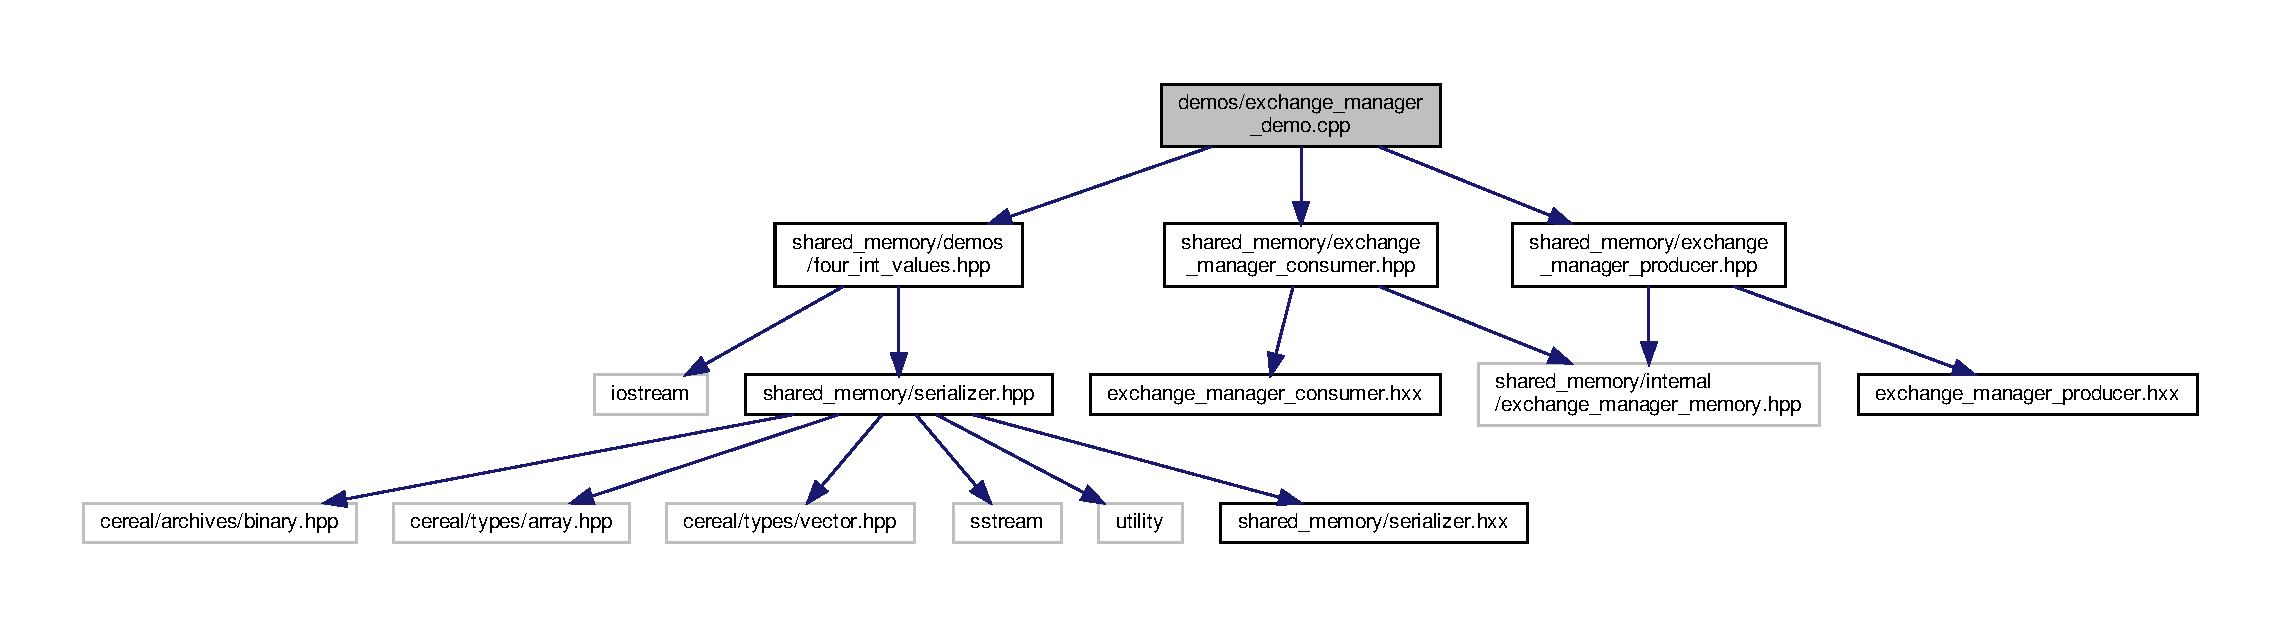
\includegraphics[width=350pt]{exchange__manager__demo_8cpp__incl}
\end{center}
\end{figure}
\subsection*{Macros}
\begin{DoxyCompactItemize}
\item 
\#define {\bfseries S\+E\+G\+M\+E\+N\+T\+\_\+\+ID}~\char`\"{}exchange\+\_\+manager\+\_\+segment\char`\"{}\hypertarget{exchange__manager__demo_8cpp_aa2341624eba49f3cdec3d9656b97cd79}{}\label{exchange__manager__demo_8cpp_aa2341624eba49f3cdec3d9656b97cd79}

\item 
\#define {\bfseries O\+B\+J\+E\+C\+T\+\_\+\+ID}~\char`\"{}exchange\+\_\+manager\+\_\+object\char`\"{}\hypertarget{exchange__manager__demo_8cpp_a7996b622059a5fb225b909180b1d385e}{}\label{exchange__manager__demo_8cpp_a7996b622059a5fb225b909180b1d385e}

\item 
\#define {\bfseries M\+A\+X\+\_\+\+E\+X\+C\+H\+A\+N\+G\+E\+\_\+\+S\+I\+ZE}~10\hypertarget{exchange__manager__demo_8cpp_ae37ce4f75418c585e844cbbbfab616c9}{}\label{exchange__manager__demo_8cpp_ae37ce4f75418c585e844cbbbfab616c9}

\end{DoxyCompactItemize}
\subsection*{Functions}
\begin{DoxyCompactItemize}
\item 
int {\bfseries main} ()\hypertarget{exchange__manager__demo_8cpp_ae66f6b31b5ad750f1fe042a706a4e3d4}{}\label{exchange__manager__demo_8cpp_ae66f6b31b5ad750f1fe042a706a4e3d4}

\end{DoxyCompactItemize}


\subsection{Detailed Description}
Demonstrate the use of the exhange manager. 

\begin{DoxyAuthor}{Author}
Vincent Berenz 
\end{DoxyAuthor}
\begin{DoxyRefDesc}{License}
\item[\hyperlink{license__license000012}{License}]License B\+S\+D-\/3-\/\+Clause \end{DoxyRefDesc}
\begin{DoxyCopyright}{Copyright}
Copyright (c) 2019, New York University and Max Planck Gesellschaft. 
\end{DoxyCopyright}
\begin{DoxyDate}{Date}
2019-\/05-\/22 
\end{DoxyDate}

\hypertarget{exchange__manager__producer_8cpp}{}\section{demos/exchange\+\_\+manager\+\_\+producer.cpp File Reference}
\label{exchange__manager__producer_8cpp}\index{demos/exchange\+\_\+manager\+\_\+producer.\+cpp@{demos/exchange\+\_\+manager\+\_\+producer.\+cpp}}


Demonstrate the use of the exhange manager producer.  


{\ttfamily \#include \char`\"{}shared\+\_\+memory/exchange\+\_\+manager\+\_\+producer.\+hpp\char`\"{}}\newline
{\ttfamily \#include $<$signal.\+h$>$}\newline
{\ttfamily \#include $<$stdlib.\+h$>$}\newline
{\ttfamily \#include $<$time.\+h$>$}\newline
{\ttfamily \#include $<$unistd.\+h$>$}\newline
{\ttfamily \#include $<$iostream$>$}\newline
{\ttfamily \#include \char`\"{}shared\+\_\+memory/demos/four\+\_\+int\+\_\+values.\+hpp\char`\"{}}\newline
{\ttfamily \#include \char`\"{}shared\+\_\+memory/exchange\+\_\+manager\+\_\+consumer.\+hpp\char`\"{}}\newline
Include dependency graph for exchange\+\_\+manager\+\_\+producer.\+cpp\+:
\nopagebreak
\begin{figure}[H]
\begin{center}
\leavevmode
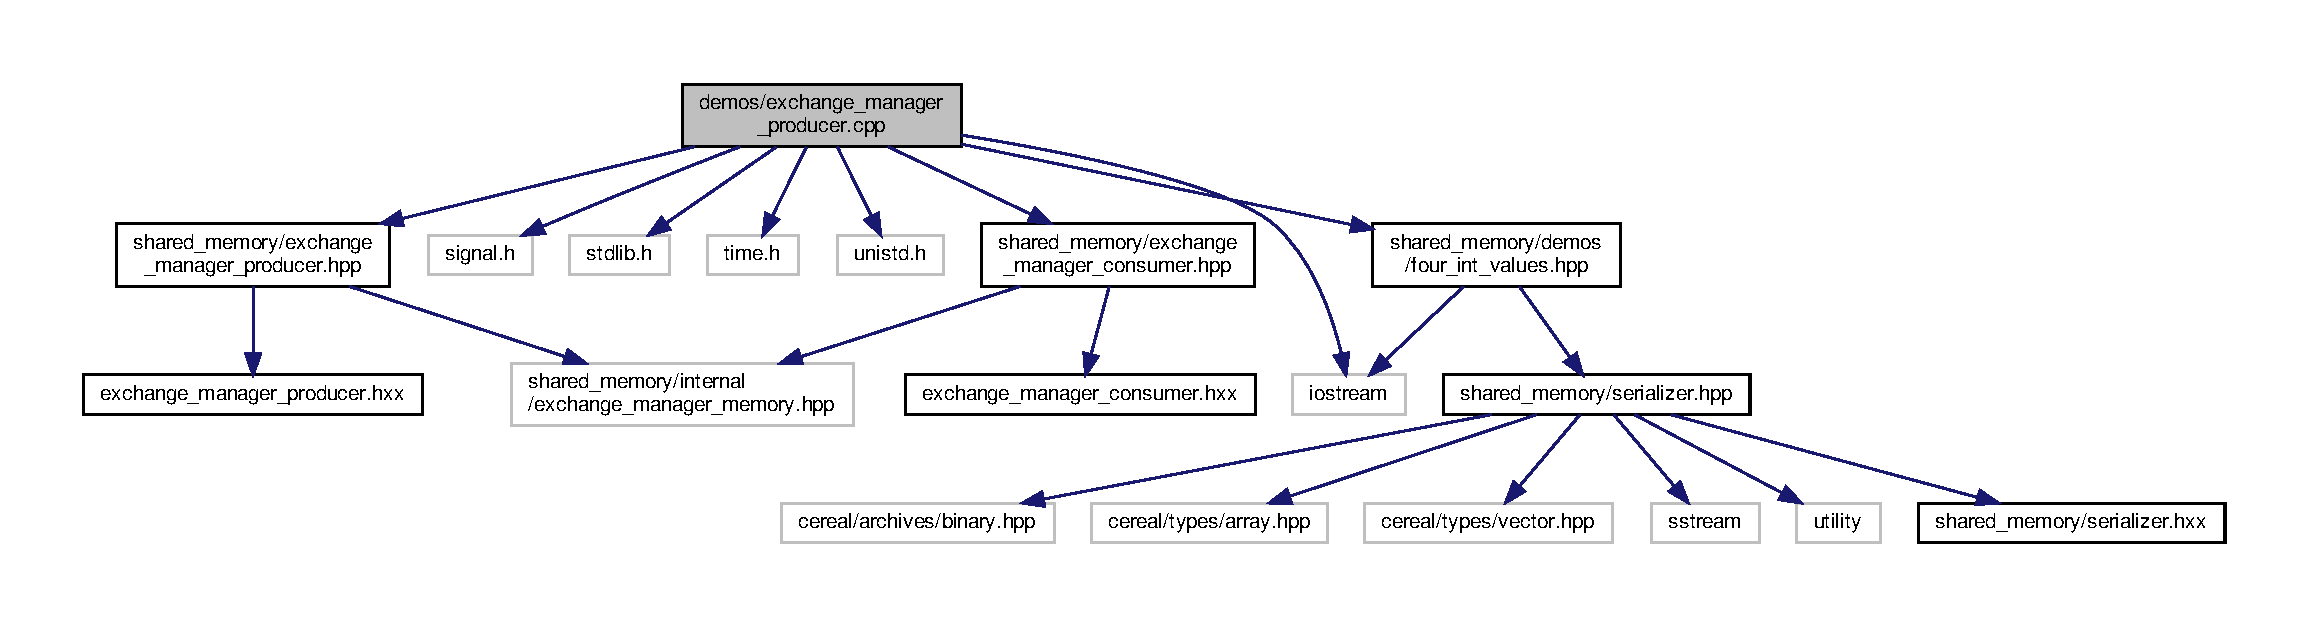
\includegraphics[width=350pt]{exchange__manager__producer_8cpp__incl}
\end{center}
\end{figure}
\subsection*{Macros}
\begin{DoxyCompactItemize}
\item 
\mbox{\Hypertarget{exchange__manager__producer_8cpp_aa2341624eba49f3cdec3d9656b97cd79}\label{exchange__manager__producer_8cpp_aa2341624eba49f3cdec3d9656b97cd79}} 
\#define {\bfseries S\+E\+G\+M\+E\+N\+T\+\_\+\+ID}~\char`\"{}exchange\+\_\+demo\+\_\+segment\char`\"{}
\item 
\mbox{\Hypertarget{exchange__manager__producer_8cpp_a7996b622059a5fb225b909180b1d385e}\label{exchange__manager__producer_8cpp_a7996b622059a5fb225b909180b1d385e}} 
\#define {\bfseries O\+B\+J\+E\+C\+T\+\_\+\+ID}~\char`\"{}exchange\+\_\+demo\+\_\+object\char`\"{}
\item 
\mbox{\Hypertarget{exchange__manager__producer_8cpp_a142810068f1b99cd93d3fc9f0e160e02}\label{exchange__manager__producer_8cpp_a142810068f1b99cd93d3fc9f0e160e02}} 
\#define {\bfseries Q\+U\+E\+U\+E\+\_\+\+S\+I\+ZE}~2000 $\ast$ 4
\end{DoxyCompactItemize}
\subsection*{Functions}
\begin{DoxyCompactItemize}
\item 
\mbox{\Hypertarget{exchange__manager__producer_8cpp_aba399b0a6a6e3bd37af95bd04e8def6f}\label{exchange__manager__producer_8cpp_aba399b0a6a6e3bd37af95bd04e8def6f}} 
void {\bfseries stop} (int)
\item 
\mbox{\Hypertarget{exchange__manager__producer_8cpp_ab70ba22b8b39e28b7981ffa998f84027}\label{exchange__manager__producer_8cpp_ab70ba22b8b39e28b7981ffa998f84027}} 
static int {\bfseries \+\_\+get\+\_\+int} (int max)
\item 
\mbox{\Hypertarget{exchange__manager__producer_8cpp_a61af3e60b94ae3e748f6fbac1e794af7}\label{exchange__manager__producer_8cpp_a61af3e60b94ae3e748f6fbac1e794af7}} 
void {\bfseries execute} ()
\item 
\mbox{\Hypertarget{exchange__manager__producer_8cpp_ae66f6b31b5ad750f1fe042a706a4e3d4}\label{exchange__manager__producer_8cpp_ae66f6b31b5ad750f1fe042a706a4e3d4}} 
int {\bfseries main} ()
\end{DoxyCompactItemize}
\subsection*{Variables}
\begin{DoxyCompactItemize}
\item 
\mbox{\Hypertarget{exchange__manager__producer_8cpp_a383e703fc3e9dd425f075cf463ee4c5b}\label{exchange__manager__producer_8cpp_a383e703fc3e9dd425f075cf463ee4c5b}} 
static bool {\bfseries R\+U\+N\+N\+I\+NG} = true
\end{DoxyCompactItemize}


\subsection{Detailed Description}
Demonstrate the use of the exhange manager producer. 

\begin{DoxyAuthor}{Author}
Vincent Berenz 
\end{DoxyAuthor}
\begin{DoxyRefDesc}{License}
\item[\hyperlink{license__license000013}{License}]License B\+S\+D-\/3-\/\+Clause \end{DoxyRefDesc}
\begin{DoxyCopyright}{Copyright}
Copyright (c) 2019, New York University and Max Planck Gesellschaft. 
\end{DoxyCopyright}
\begin{DoxyDate}{Date}
2019-\/05-\/22 
\end{DoxyDate}

\hypertarget{four__int__values_8cpp}{}\section{demos/four\+\_\+int\+\_\+values.cpp File Reference}
\label{four__int__values_8cpp}\index{demos/four\+\_\+int\+\_\+values.\+cpp@{demos/four\+\_\+int\+\_\+values.\+cpp}}


Demonstrate how to create a message with the exchange manager.  


{\ttfamily \#include \char`\"{}shared\+\_\+memory/demos/four\+\_\+int\+\_\+values.\+hpp\char`\"{}}\\*
Include dependency graph for four\+\_\+int\+\_\+values.\+cpp\+:
\nopagebreak
\begin{figure}[H]
\begin{center}
\leavevmode
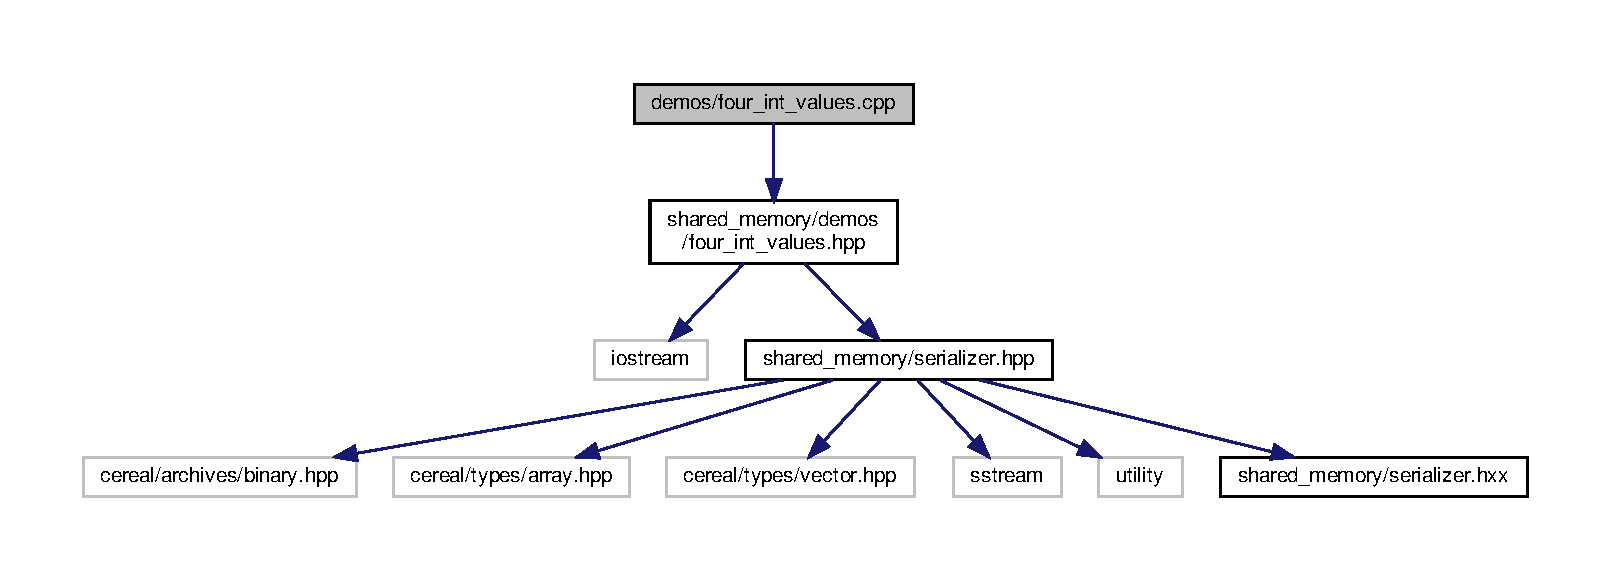
\includegraphics[width=350pt]{four__int__values_8cpp__incl}
\end{center}
\end{figure}
\subsection*{Namespaces}
\begin{DoxyCompactItemize}
\item 
 \hyperlink{namespaceshared__memory}{shared\+\_\+memory}
\begin{DoxyCompactList}\small\item\em All templated types in this namespaces are elementary types\+: int, double, float, char$\ast$, ... \end{DoxyCompactList}\end{DoxyCompactItemize}


\subsection{Detailed Description}
Demonstrate how to create a message with the exchange manager. 

\begin{DoxyAuthor}{Author}
Vincent Berenz 
\end{DoxyAuthor}
\begin{DoxyRefDesc}{License}
\item[\hyperlink{license__license000014}{License}]License B\+S\+D-\/3-\/\+Clause \end{DoxyRefDesc}
\begin{DoxyCopyright}{Copyright}
Copyright (c) 2019, New York University and Max Planck Gesellschaft. 
\end{DoxyCopyright}
\begin{DoxyDate}{Date}
2019-\/05-\/22 
\end{DoxyDate}

\hypertarget{get__data_8cpp}{}\section{demos/get\+\_\+data.cpp File Reference}
\label{get__data_8cpp}\index{demos/get\+\_\+data.\+cpp@{demos/get\+\_\+data.\+cpp}}


Create a small app that fetch the data from a shared memory. This memory is filled with the counter part of this app\+: set\+\_\+data.  


{\ttfamily \#include $<$signal.\+h$>$}\\*
{\ttfamily \#include $<$unistd.\+h$>$}\\*
{\ttfamily \#include $<$iostream$>$}\\*
{\ttfamily \#include $<$vector$>$}\\*
{\ttfamily \#include \char`\"{}shared\+\_\+memory/shared\+\_\+memory.\+hpp\char`\"{}}\\*
Include dependency graph for get\+\_\+data.\+cpp\+:
\nopagebreak
\begin{figure}[H]
\begin{center}
\leavevmode
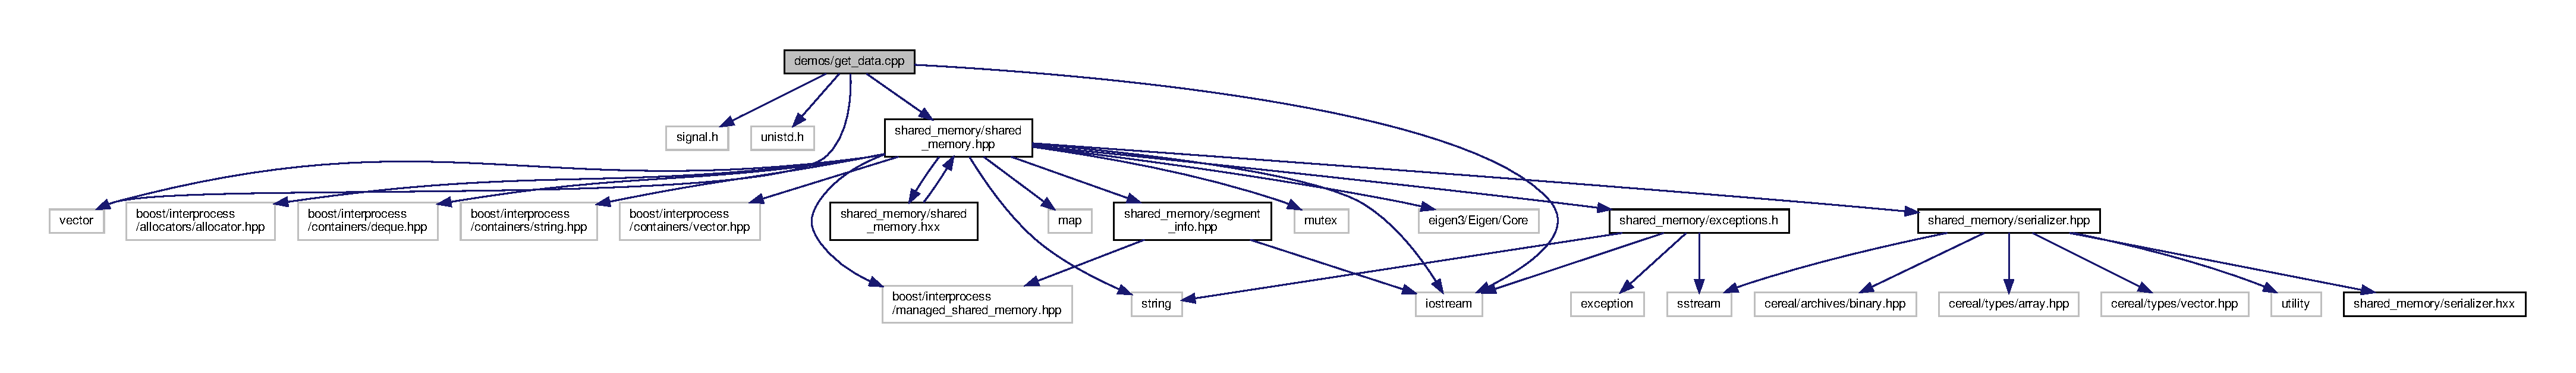
\includegraphics[width=350pt]{get__data_8cpp__incl}
\end{center}
\end{figure}
\subsection*{Functions}
\begin{DoxyCompactItemize}
\item 
void {\bfseries exiting\+\_\+memory} (int)\hypertarget{get__data_8cpp_a054fcc6a68c958f06aa76c177317c483}{}\label{get__data_8cpp_a054fcc6a68c958f06aa76c177317c483}

\item 
int {\bfseries main} ()\hypertarget{get__data_8cpp_ae66f6b31b5ad750f1fe042a706a4e3d4}{}\label{get__data_8cpp_ae66f6b31b5ad750f1fe042a706a4e3d4}

\end{DoxyCompactItemize}
\subsection*{Variables}
\begin{DoxyCompactItemize}
\item 
static bool {\bfseries R\+U\+N\+N\+I\+NG} = true\hypertarget{get__data_8cpp_a383e703fc3e9dd425f075cf463ee4c5b}{}\label{get__data_8cpp_a383e703fc3e9dd425f075cf463ee4c5b}

\end{DoxyCompactItemize}


\subsection{Detailed Description}
Create a small app that fetch the data from a shared memory. This memory is filled with the counter part of this app\+: set\+\_\+data. 

\begin{DoxyAuthor}{Author}
Vincent Berenz 
\end{DoxyAuthor}
\begin{DoxyRefDesc}{License}
\item[\hyperlink{license__license000015}{License}]License B\+S\+D-\/3-\/\+Clause \end{DoxyRefDesc}
\begin{DoxyCopyright}{Copyright}
Copyright (c) 2019, New York University and Max Planck Gesellschaft. 
\end{DoxyCopyright}
\begin{DoxyDate}{Date}
2019-\/05-\/22 
\end{DoxyDate}

\hypertarget{set__data_8cpp}{}\section{demos/set\+\_\+data.cpp File Reference}
\label{set__data_8cpp}\index{demos/set\+\_\+data.\+cpp@{demos/set\+\_\+data.\+cpp}}


shows how to serialize an instance of a class with an eigen matrix as attribute  


{\ttfamily \#include $<$signal.\+h$>$}\\*
{\ttfamily \#include $<$unistd.\+h$>$}\\*
{\ttfamily \#include $<$iostream$>$}\\*
{\ttfamily \#include $<$vector$>$}\\*
{\ttfamily \#include \char`\"{}shared\+\_\+memory/shared\+\_\+memory.\+hpp\char`\"{}}\\*
Include dependency graph for set\+\_\+data.\+cpp\+:
\nopagebreak
\begin{figure}[H]
\begin{center}
\leavevmode
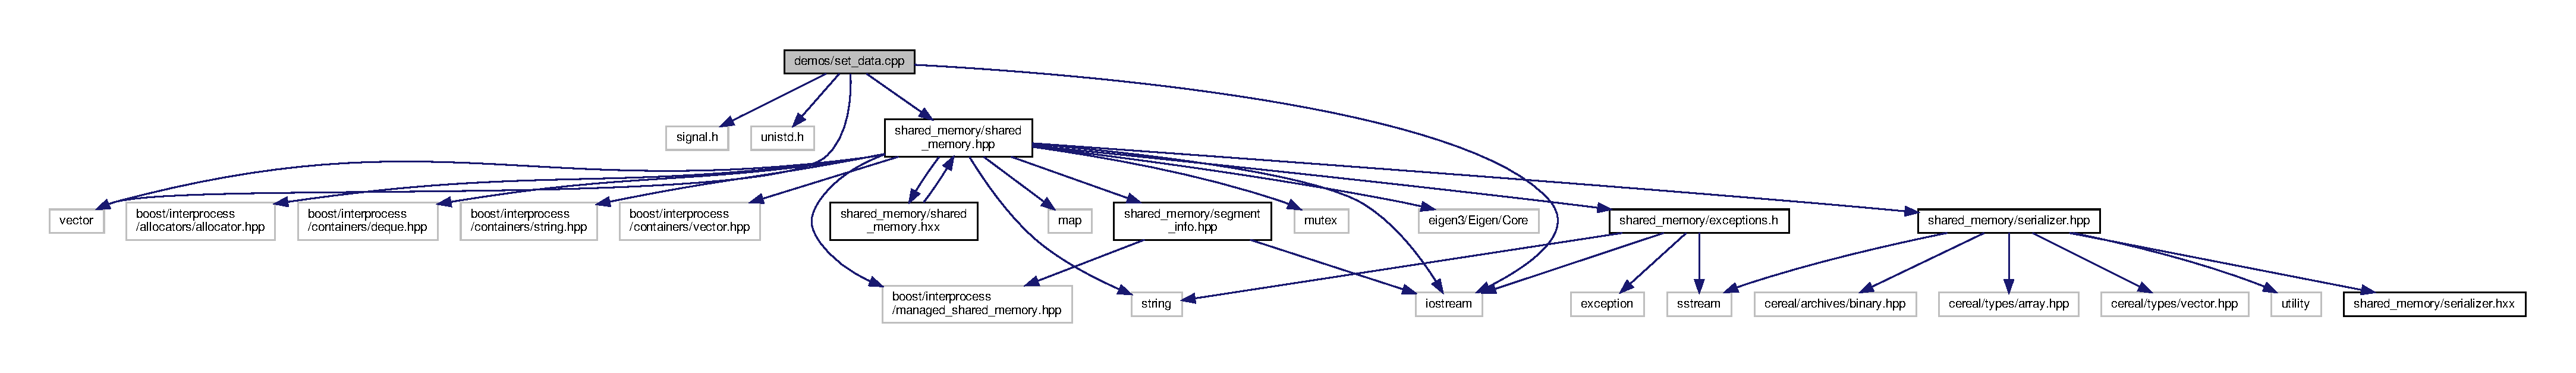
\includegraphics[width=350pt]{set__data_8cpp__incl}
\end{center}
\end{figure}
\subsection*{Functions}
\begin{DoxyCompactItemize}
\item 
void {\bfseries cleaning\+\_\+memory} (int)\hypertarget{set__data_8cpp_a5d2be5fb88fef648640fe973785d58b1}{}\label{set__data_8cpp_a5d2be5fb88fef648640fe973785d58b1}

\item 
int {\bfseries main} ()\hypertarget{set__data_8cpp_ae66f6b31b5ad750f1fe042a706a4e3d4}{}\label{set__data_8cpp_ae66f6b31b5ad750f1fe042a706a4e3d4}

\end{DoxyCompactItemize}
\subsection*{Variables}
\begin{DoxyCompactItemize}
\item 
static bool {\bfseries R\+U\+N\+N\+I\+NG} = true\hypertarget{set__data_8cpp_a383e703fc3e9dd425f075cf463ee4c5b}{}\label{set__data_8cpp_a383e703fc3e9dd425f075cf463ee4c5b}

\end{DoxyCompactItemize}


\subsection{Detailed Description}
shows how to serialize an instance of a class with an eigen matrix as attribute 

Create a small app that set the data into a shared memory. This memory is read from the counter part of this app\+: get\+\_\+data.

shows how to turn of console prints

\begin{DoxyAuthor}{Author}
Vincent Berenz 
\end{DoxyAuthor}
\begin{DoxyRefDesc}{License}
\item[\hyperlink{license__license000009}{License}]License B\+S\+D-\/3-\/\+Clause \end{DoxyRefDesc}
\begin{DoxyCopyright}{Copyright}
Copyright (c) 2019, New York University and Max Planck Gesellschaft. 
\end{DoxyCopyright}
\begin{DoxyDate}{Date}
2019-\/05-\/22
\end{DoxyDate}
\begin{DoxyAuthor}{Author}
Vincent Berenz 
\end{DoxyAuthor}
\begin{DoxyRefDesc}{License}
\item[\hyperlink{license__license000010}{License}]License B\+S\+D-\/3-\/\+Clause \end{DoxyRefDesc}
\begin{DoxyCopyright}{Copyright}
Copyright (c) 2019, New York University and Max Planck Gesellschaft. 
\end{DoxyCopyright}
\begin{DoxyDate}{Date}
2019-\/05-\/22
\end{DoxyDate}
\begin{DoxyAuthor}{Author}
Vincent Berenz 
\end{DoxyAuthor}
\begin{DoxyRefDesc}{License}
\item[\hyperlink{license__license000016}{License}]License B\+S\+D-\/3-\/\+Clause \end{DoxyRefDesc}
\begin{DoxyCopyright}{Copyright}
Copyright (c) 2019, New York University and Max Planck Gesellschaft. 
\end{DoxyCopyright}
\begin{DoxyDate}{Date}
2019-\/05-\/22 
\end{DoxyDate}

\hypertarget{std__string__vector_8cpp}{}\section{demos/std\+\_\+string\+\_\+vector.cpp File Reference}
\label{std__string__vector_8cpp}\index{demos/std\+\_\+string\+\_\+vector.\+cpp@{demos/std\+\_\+string\+\_\+vector.\+cpp}}


This demonstrate how to use the equivalent of std\+::string in the shared memory.  


{\ttfamily \#include $<$boost/interprocess/allocators/allocator.\+hpp$>$}\newline
{\ttfamily \#include $<$boost/interprocess/containers/string.\+hpp$>$}\newline
{\ttfamily \#include $<$boost/interprocess/containers/vector.\+hpp$>$}\newline
{\ttfamily \#include $<$boost/interprocess/managed\+\_\+shared\+\_\+memory.\+hpp$>$}\newline
Include dependency graph for std\+\_\+string\+\_\+vector.\+cpp\+:
\nopagebreak
\begin{figure}[H]
\begin{center}
\leavevmode
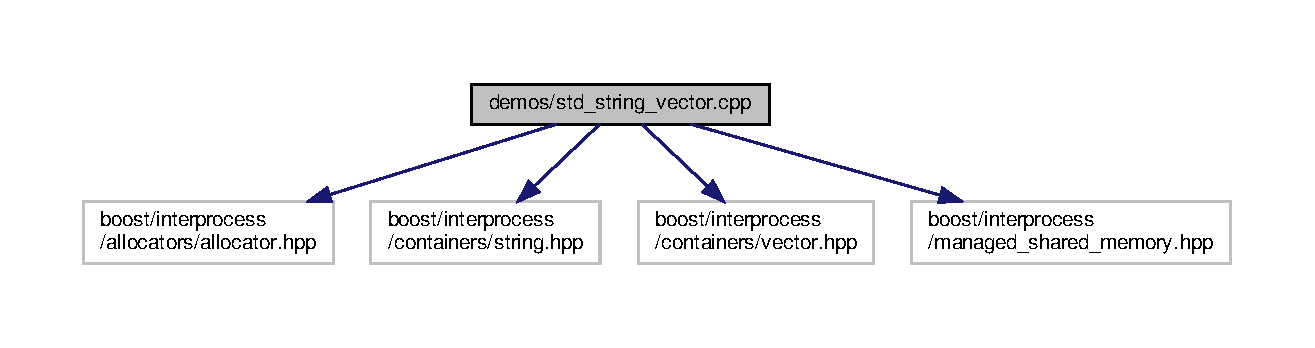
\includegraphics[width=350pt]{std__string__vector_8cpp__incl}
\end{center}
\end{figure}
\subsection*{Functions}
\begin{DoxyCompactItemize}
\item 
\mbox{\Hypertarget{std__string__vector_8cpp_ae66f6b31b5ad750f1fe042a706a4e3d4}\label{std__string__vector_8cpp_ae66f6b31b5ad750f1fe042a706a4e3d4}} 
int {\bfseries main} ()
\end{DoxyCompactItemize}


\subsection{Detailed Description}
This demonstrate how to use the equivalent of std\+::string in the shared memory. 

\begin{DoxyAuthor}{Author}
Vincent Berenz 
\end{DoxyAuthor}
\begin{DoxyRefDesc}{License}
\item[\hyperlink{license__license000017}{License}]License B\+S\+D-\/3-\/\+Clause \end{DoxyRefDesc}
\begin{DoxyCopyright}{Copyright}
Copyright (c) 2019, New York University and Max Planck Gesellschaft. 
\end{DoxyCopyright}
\begin{DoxyDate}{Date}
2019-\/05-\/22 
\end{DoxyDate}

\hypertarget{benchmark__common_8hh}{}\section{include/shared\+\_\+memory/benchmarks/benchmark\+\_\+common.hh File Reference}
\label{benchmark__common_8hh}\index{include/shared\+\_\+memory/benchmarks/benchmark\+\_\+common.\+hh@{include/shared\+\_\+memory/benchmarks/benchmark\+\_\+common.\+hh}}


Common tools for benchmarking.  


{\ttfamily \#include $<$signal.\+h$>$}\newline
{\ttfamily \#include $<$unistd.\+h$>$}\newline
{\ttfamily \#include $<$chrono$>$}\newline
{\ttfamily \#include $<$cmath$>$}\newline
{\ttfamily \#include $<$iostream$>$}\newline
{\ttfamily \#include $<$vector$>$}\newline
Include dependency graph for benchmark\+\_\+common.\+hh\+:
\nopagebreak
\begin{figure}[H]
\begin{center}
\leavevmode
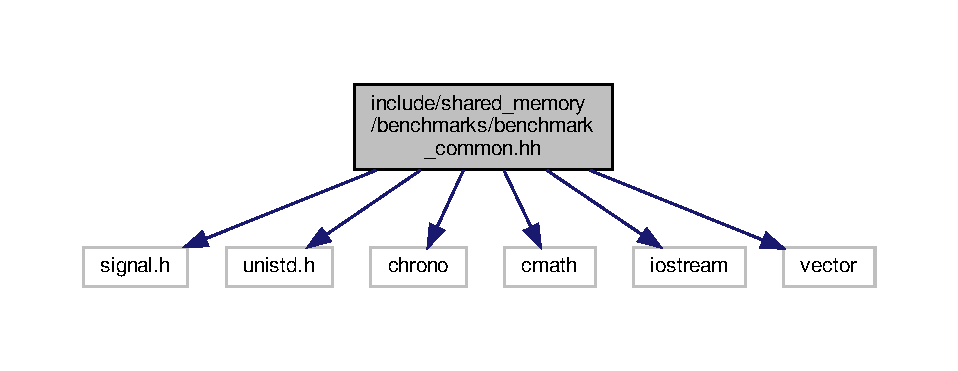
\includegraphics[width=350pt]{benchmark__common_8hh__incl}
\end{center}
\end{figure}
This graph shows which files directly or indirectly include this file\+:
\nopagebreak
\begin{figure}[H]
\begin{center}
\leavevmode
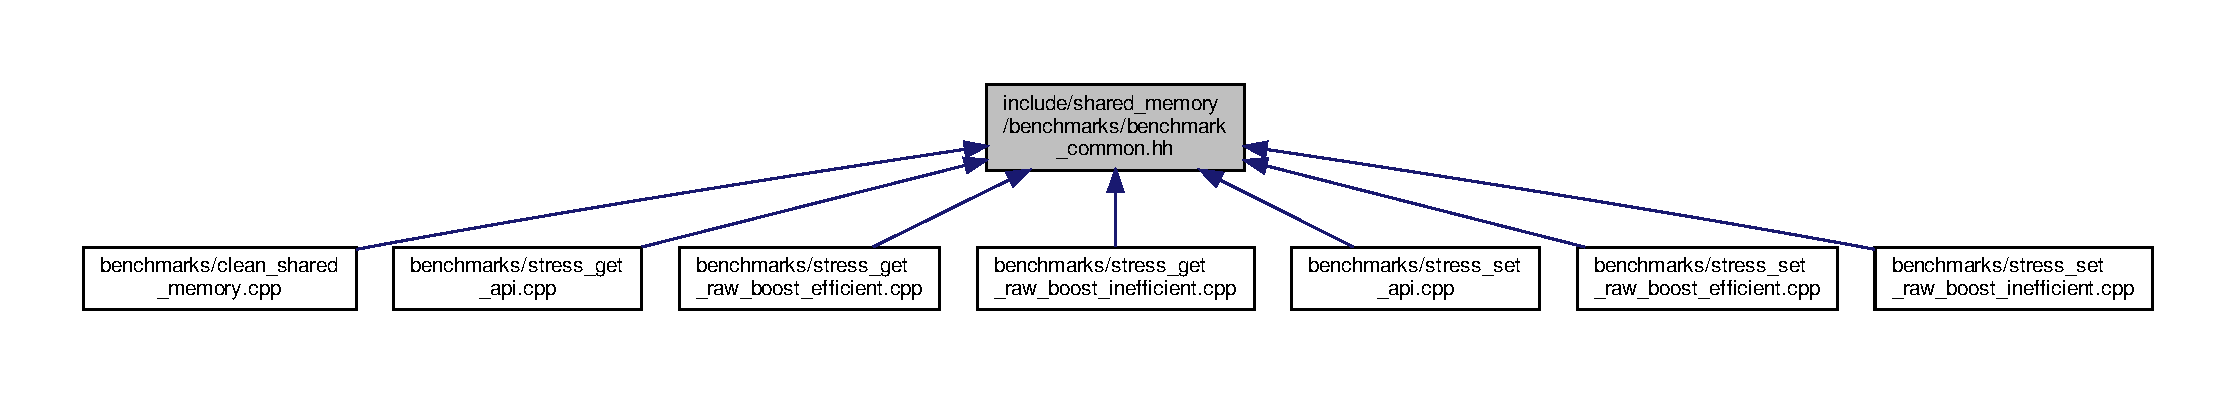
\includegraphics[width=350pt]{benchmark__common_8hh__dep__incl}
\end{center}
\end{figure}
\subsection*{Classes}
\begin{DoxyCompactItemize}
\item 
struct \hyperlink{structMeasureTime}{Measure\+Time}
\end{DoxyCompactItemize}
\subsection*{Macros}
\begin{DoxyCompactItemize}
\item 
\mbox{\Hypertarget{benchmark__common_8hh_a21a16aec41293c80beb10d71f79ad7a2}\label{benchmark__common_8hh_a21a16aec41293c80beb10d71f79ad7a2}} 
\#define {\bfseries S\+H\+A\+R\+E\+D\+\_\+\+M\+E\+M\+O\+R\+Y\+\_\+\+S\+I\+ZE}~65536
\item 
\mbox{\Hypertarget{benchmark__common_8hh_a70ed59adcb4159ac551058053e649640}\label{benchmark__common_8hh_a70ed59adcb4159ac551058053e649640}} 
\#define {\bfseries S\+I\+ZE}~1000
\item 
\mbox{\Hypertarget{benchmark__common_8hh_adf00b55c2043a89ad0ac69b3a2428281}\label{benchmark__common_8hh_adf00b55c2043a89ad0ac69b3a2428281}} 
\#define {\bfseries N\+U\+M\+B\+E\+R\+\_\+\+O\+R\+\_\+\+M\+E\+A\+S\+U\+R\+E\+D\+\_\+\+I\+T\+E\+R\+A\+T\+I\+O\+NS}~1000
\item 
\mbox{\Hypertarget{benchmark__common_8hh_adc5fa90d9af8c15b5dc4c72697821c36}\label{benchmark__common_8hh_adc5fa90d9af8c15b5dc4c72697821c36}} 
\#define {\bfseries M\+A\+X\+\_\+\+N\+U\+N\+M\+B\+E\+R\+\_\+\+O\+F\+\_\+\+I\+T\+E\+R\+A\+T\+I\+ON}~10000
\end{DoxyCompactItemize}
\subsection*{Typedefs}
\begin{DoxyCompactItemize}
\item 
\mbox{\Hypertarget{benchmark__common_8hh_ac3379ce076aff9d7667b3fc267a87f48}\label{benchmark__common_8hh_ac3379ce076aff9d7667b3fc267a87f48}} 
typedef std\+::chrono\+::high\+\_\+resolution\+\_\+clock\+::time\+\_\+point {\bfseries Time\+Type}
\end{DoxyCompactItemize}
\subsection*{Functions}
\begin{DoxyCompactItemize}
\item 
\mbox{\Hypertarget{benchmark__common_8hh_a59c33a6b3ce646e26614a12d0193a2bd}\label{benchmark__common_8hh_a59c33a6b3ce646e26614a12d0193a2bd}} 
static std\+::vector$<$ double $>$ {\bfseries D\+A\+TA} (S\+I\+ZE, 2)
\item 
\mbox{\Hypertarget{benchmark__common_8hh_a2eab504a26ce27f25dc75a77486f0291}\label{benchmark__common_8hh_a2eab504a26ce27f25dc75a77486f0291}} 
static std\+::string {\bfseries S\+H\+M\+\_\+\+N\+A\+ME} (\char`\"{}stress\+\_\+test\char`\"{})
\item 
\mbox{\Hypertarget{benchmark__common_8hh_a7b0c439ad35b06a4ef0180f55a6d005a}\label{benchmark__common_8hh_a7b0c439ad35b06a4ef0180f55a6d005a}} 
static std\+::string {\bfseries S\+H\+M\+\_\+\+O\+B\+J\+E\+C\+T\+\_\+\+N\+A\+ME} (\char`\"{}stress\+\_\+object\char`\"{})
\item 
\mbox{\Hypertarget{benchmark__common_8hh_a8dd0271b9a992c4b761972f7082052a0}\label{benchmark__common_8hh_a8dd0271b9a992c4b761972f7082052a0}} 
std\+::ostream \& {\bfseries operator$<$$<$} (std\+::ostream \&os, const \hyperlink{structMeasureTime}{Measure\+Time} \&time)
\item 
\mbox{\Hypertarget{benchmark__common_8hh_aa10d0d36e9613185c60cd04e376e12bc}\label{benchmark__common_8hh_aa10d0d36e9613185c60cd04e376e12bc}} 
void {\bfseries init\+\_\+benchmark} ()
\item 
\mbox{\Hypertarget{benchmark__common_8hh_a91d65608f8757f45d8db7c6e58dfe9f4}\label{benchmark__common_8hh_a91d65608f8757f45d8db7c6e58dfe9f4}} 
void {\bfseries code\+\_\+to\+\_\+benchamrk} ()
\item 
\mbox{\Hypertarget{benchmark__common_8hh_a3ae3ecd5464dfa055c802feb243e62d9}\label{benchmark__common_8hh_a3ae3ecd5464dfa055c802feb243e62d9}} 
void {\bfseries end\+\_\+benchmark} ()
\end{DoxyCompactItemize}
\subsection*{Variables}
\begin{DoxyCompactItemize}
\item 
\mbox{\Hypertarget{benchmark__common_8hh_a383e703fc3e9dd425f075cf463ee4c5b}\label{benchmark__common_8hh_a383e703fc3e9dd425f075cf463ee4c5b}} 
bool {\bfseries R\+U\+N\+N\+I\+NG}
\end{DoxyCompactItemize}


\subsection{Detailed Description}
Common tools for benchmarking. 

\begin{DoxyAuthor}{Author}
Vincent Berenz 
\end{DoxyAuthor}
\begin{DoxyRefDesc}{License}
\item[\hyperlink{license__license000018}{License}]License B\+S\+D-\/3-\/\+Clause \end{DoxyRefDesc}
\begin{DoxyCopyright}{Copyright}
Copyright (c) 2019, New York University and Max Planck Gesellschaft. 
\end{DoxyCopyright}
\begin{DoxyDate}{Date}
2019-\/05-\/22 
\end{DoxyDate}

\hypertarget{four__int__values_8hpp}{}\section{include/shared\+\_\+memory/demos/four\+\_\+int\+\_\+values.hpp File Reference}
\label{four__int__values_8hpp}\index{include/shared\+\_\+memory/demos/four\+\_\+int\+\_\+values.\+hpp@{include/shared\+\_\+memory/demos/four\+\_\+int\+\_\+values.\+hpp}}


o $\ast$  


{\ttfamily \#include $<$iostream$>$}\newline
{\ttfamily \#include \char`\"{}shared\+\_\+memory/serializer.\+hpp\char`\"{}}\newline
Include dependency graph for four\+\_\+int\+\_\+values.\+hpp\+:
\nopagebreak
\begin{figure}[H]
\begin{center}
\leavevmode
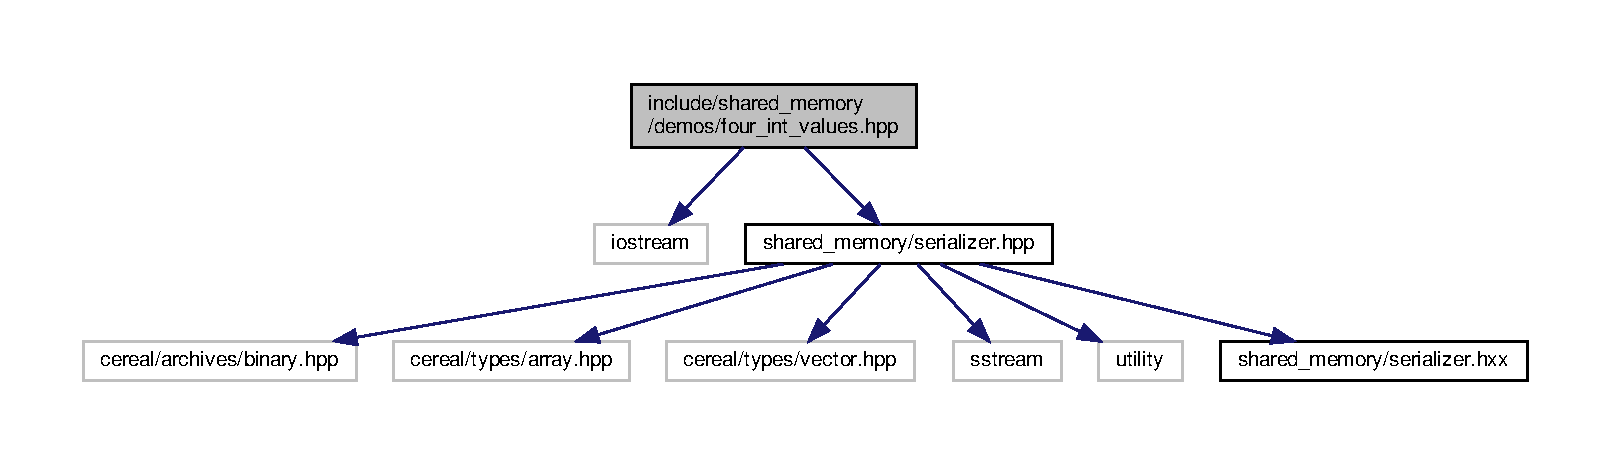
\includegraphics[width=350pt]{four__int__values_8hpp__incl}
\end{center}
\end{figure}
This graph shows which files directly or indirectly include this file\+:
\nopagebreak
\begin{figure}[H]
\begin{center}
\leavevmode
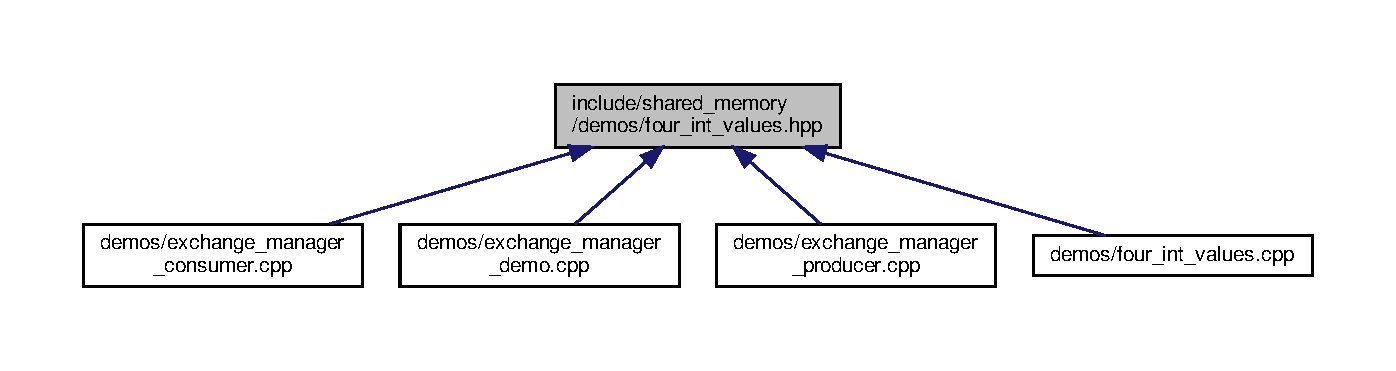
\includegraphics[width=350pt]{four__int__values_8hpp__dep__incl}
\end{center}
\end{figure}
\subsection*{Classes}
\begin{DoxyCompactItemize}
\item 
class \hyperlink{classshared__memory_1_1Four__int__values}{shared\+\_\+memory\+::\+Four\+\_\+int\+\_\+values}
\begin{DoxyCompactList}\small\item\em Example of an instance that can be serialized. \end{DoxyCompactList}\end{DoxyCompactItemize}
\subsection*{Namespaces}
\begin{DoxyCompactItemize}
\item 
 \hyperlink{namespaceshared__memory}{shared\+\_\+memory}
\begin{DoxyCompactList}\small\item\em All templated types in this namespaces are elementary types\+: int, double, float, char$\ast$, ... \end{DoxyCompactList}\end{DoxyCompactItemize}


\subsection{Detailed Description}
o $\ast$ 

\begin{DoxyAuthor}{Author}
Vincent Berenz 
\end{DoxyAuthor}
\begin{DoxyRefDesc}{License}
\item[\hyperlink{license__license000019}{License}]License B\+S\+D-\/3-\/\+Clause \end{DoxyRefDesc}
\begin{DoxyCopyright}{Copyright}
Copyright (c) 2019, New York University and Max Planck Gesellschaft. 
\end{DoxyCopyright}
\begin{DoxyDate}{Date}
2019-\/05-\/22
\end{DoxyDate}
Defines a messages to be sent throw the shared memory 
\hypertarget{exceptions_8h}{}\section{include/shared\+\_\+memory/exceptions.h File Reference}
\label{exceptions_8h}\index{include/shared\+\_\+memory/exceptions.\+h@{include/shared\+\_\+memory/exceptions.\+h}}


Defines debugging exceptions for this package.  


{\ttfamily \#include $<$exception$>$}\\*
{\ttfamily \#include $<$iostream$>$}\\*
{\ttfamily \#include $<$sstream$>$}\\*
{\ttfamily \#include $<$string$>$}\\*
Include dependency graph for exceptions.\+h\+:
\nopagebreak
\begin{figure}[H]
\begin{center}
\leavevmode
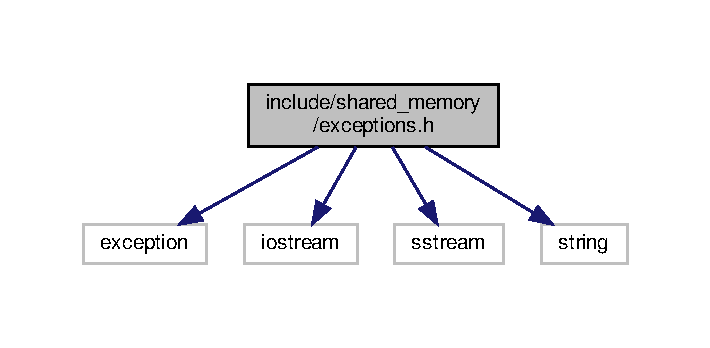
\includegraphics[width=341pt]{exceptions_8h__incl}
\end{center}
\end{figure}
This graph shows which files directly or indirectly include this file\+:
\nopagebreak
\begin{figure}[H]
\begin{center}
\leavevmode
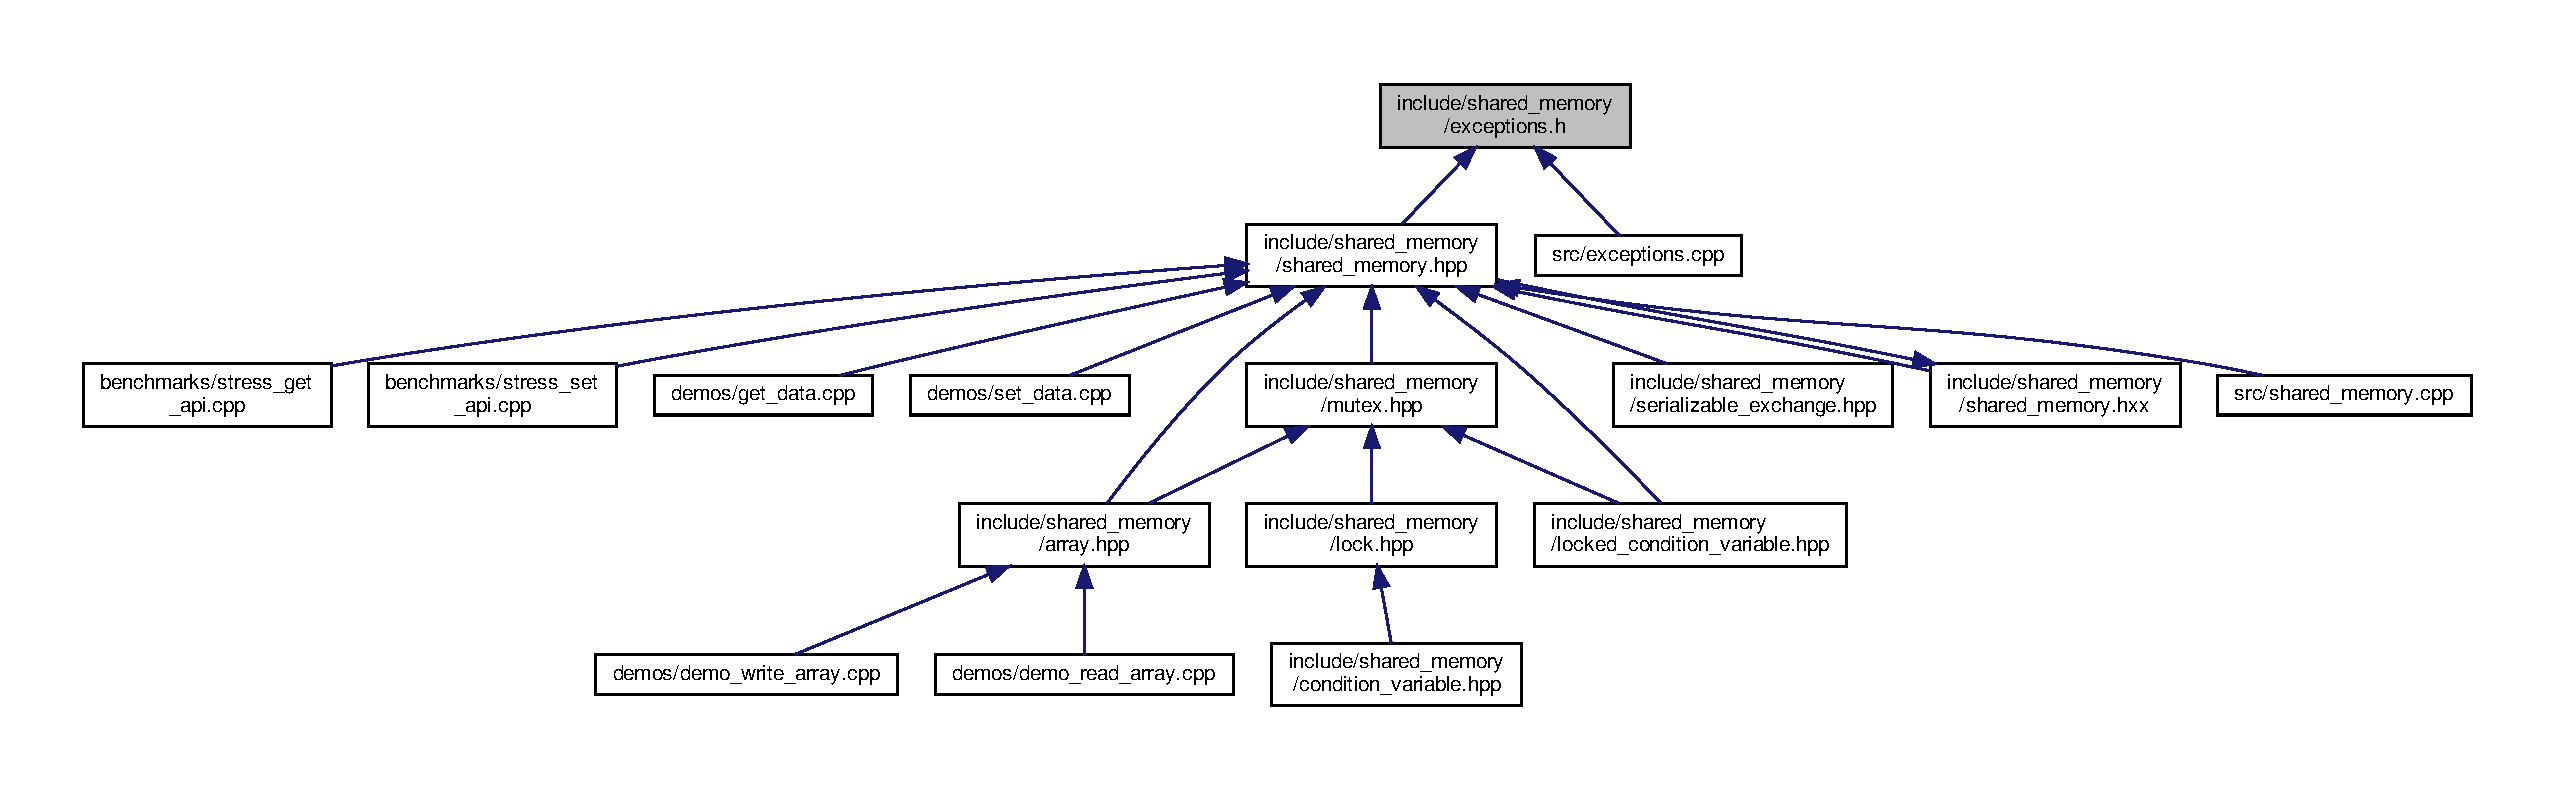
\includegraphics[width=350pt]{exceptions_8h__dep__incl}
\end{center}
\end{figure}
\subsection*{Classes}
\begin{DoxyCompactItemize}
\item 
class \hyperlink{classshared__memory_1_1Allocation__exception}{shared\+\_\+memory\+::\+Allocation\+\_\+exception}
\item 
class \hyperlink{classshared__memory_1_1Memory__overflow__exception}{shared\+\_\+memory\+::\+Memory\+\_\+overflow\+\_\+exception}
\item 
class \hyperlink{classshared__memory_1_1Unexpected__size__exception}{shared\+\_\+memory\+::\+Unexpected\+\_\+size\+\_\+exception}
\item 
class \hyperlink{classshared__memory_1_1Not__consumed__exception}{shared\+\_\+memory\+::\+Not\+\_\+consumed\+\_\+exception}
\item 
class \hyperlink{classshared__memory_1_1Unexpected__map__key}{shared\+\_\+memory\+::\+Unexpected\+\_\+map\+\_\+key$<$ Key $>$}
\end{DoxyCompactItemize}
\subsection*{Namespaces}
\begin{DoxyCompactItemize}
\item 
 \hyperlink{namespaceshared__memory}{shared\+\_\+memory}
\begin{DoxyCompactList}\small\item\em All templated types in this namespaces are elementary types\+: int, double, float, char$\ast$, ... \end{DoxyCompactList}\end{DoxyCompactItemize}


\subsection{Detailed Description}
Defines debugging exceptions for this package. 

\begin{DoxyAuthor}{Author}
Vincent Berenz 
\end{DoxyAuthor}
\begin{DoxyRefDesc}{License}
\item[\hyperlink{license__license000020}{License}]License B\+S\+D-\/3-\/\+Clause \end{DoxyRefDesc}
\begin{DoxyCopyright}{Copyright}
Copyright (c) 2019, New York University and Max Planck Gesellschaft. 
\end{DoxyCopyright}
\begin{DoxyDate}{Date}
2019-\/05-\/22 
\end{DoxyDate}

\hypertarget{exchange__manager__consumer_8hpp}{}\section{include/shared\+\_\+memory/exchange\+\_\+manager\+\_\+consumer.hpp File Reference}
\label{exchange__manager__consumer_8hpp}\index{include/shared\+\_\+memory/exchange\+\_\+manager\+\_\+consumer.\+hpp@{include/shared\+\_\+memory/exchange\+\_\+manager\+\_\+consumer.\+hpp}}


Interprocess exchange of serialized items.  


{\ttfamily \#include \char`\"{}shared\+\_\+memory/internal/exchange\+\_\+manager\+\_\+memory.\+hpp\char`\"{}}\\*
{\ttfamily \#include \char`\"{}exchange\+\_\+manager\+\_\+consumer.\+hxx\char`\"{}}\\*
Include dependency graph for exchange\+\_\+manager\+\_\+consumer.\+hpp\+:
\nopagebreak
\begin{figure}[H]
\begin{center}
\leavevmode
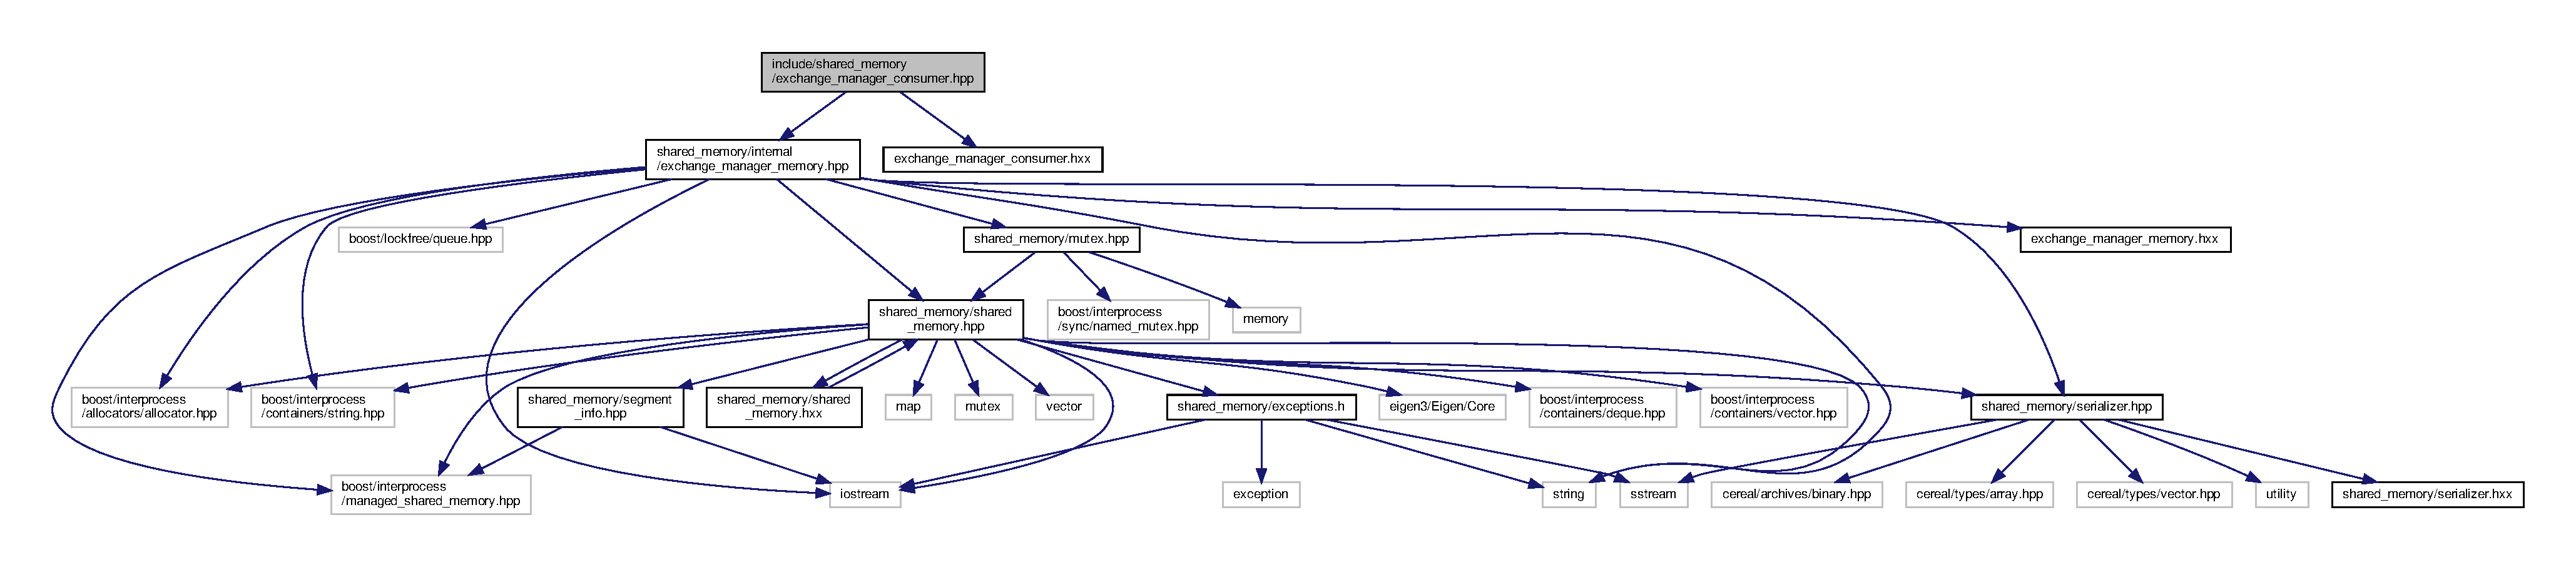
\includegraphics[width=350pt]{exchange__manager__consumer_8hpp__incl}
\end{center}
\end{figure}
This graph shows which files directly or indirectly include this file\+:
\nopagebreak
\begin{figure}[H]
\begin{center}
\leavevmode
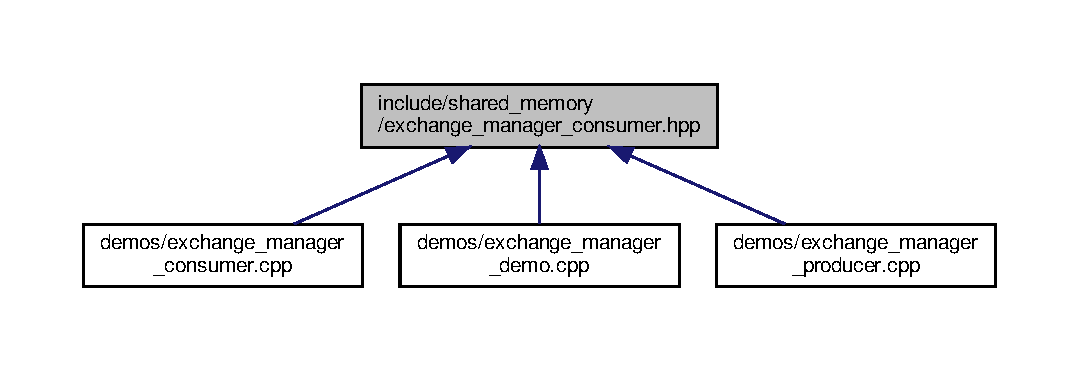
\includegraphics[width=350pt]{exchange__manager__consumer_8hpp__dep__incl}
\end{center}
\end{figure}
\subsection*{Classes}
\begin{DoxyCompactItemize}
\item 
class \hyperlink{classshared__memory_1_1Exchange__manager__consumer}{shared\+\_\+memory\+::\+Exchange\+\_\+manager\+\_\+consumer$<$ Serializable, Q\+U\+E\+U\+E\+\_\+\+S\+I\+Z\+E $>$}
\end{DoxyCompactItemize}
\subsection*{Namespaces}
\begin{DoxyCompactItemize}
\item 
 \hyperlink{namespaceshared__memory}{shared\+\_\+memory}
\begin{DoxyCompactList}\small\item\em All templated types in this namespaces are elementary types\+: int, double, float, char$\ast$, ... \end{DoxyCompactList}\end{DoxyCompactItemize}


\subsection{Detailed Description}
Interprocess exchange of serialized items. 

\begin{DoxyAuthor}{Author}
Vincent Berenz (\href{mailto:vberenz@tuebingen.mpg.de}{\tt vberenz@tuebingen.\+mpg.\+de}) 
\end{DoxyAuthor}
\begin{DoxyRefDesc}{License}
\item[\hyperlink{license__license000021}{License}]License B\+S\+D-\/3-\/\+Clause \end{DoxyRefDesc}
\begin{DoxyCopyright}{Copyright}
Copyright (c) 2019, New York University and Max Planck Gesellschaft. 
\end{DoxyCopyright}
\begin{DoxyDate}{Date}
2019-\/06-\/07 
\end{DoxyDate}

\hypertarget{exchange__manager__producer_8hpp}{}\section{include/shared\+\_\+memory/exchange\+\_\+manager\+\_\+producer.hpp File Reference}
\label{exchange__manager__producer_8hpp}\index{include/shared\+\_\+memory/exchange\+\_\+manager\+\_\+producer.\+hpp@{include/shared\+\_\+memory/exchange\+\_\+manager\+\_\+producer.\+hpp}}


Interprocess exchange of serialized items.  


{\ttfamily \#include \char`\"{}shared\+\_\+memory/internal/exchange\+\_\+manager\+\_\+memory.\+hpp\char`\"{}}\newline
{\ttfamily \#include \char`\"{}exchange\+\_\+manager\+\_\+producer.\+hxx\char`\"{}}\newline
Include dependency graph for exchange\+\_\+manager\+\_\+producer.\+hpp\+:
\nopagebreak
\begin{figure}[H]
\begin{center}
\leavevmode
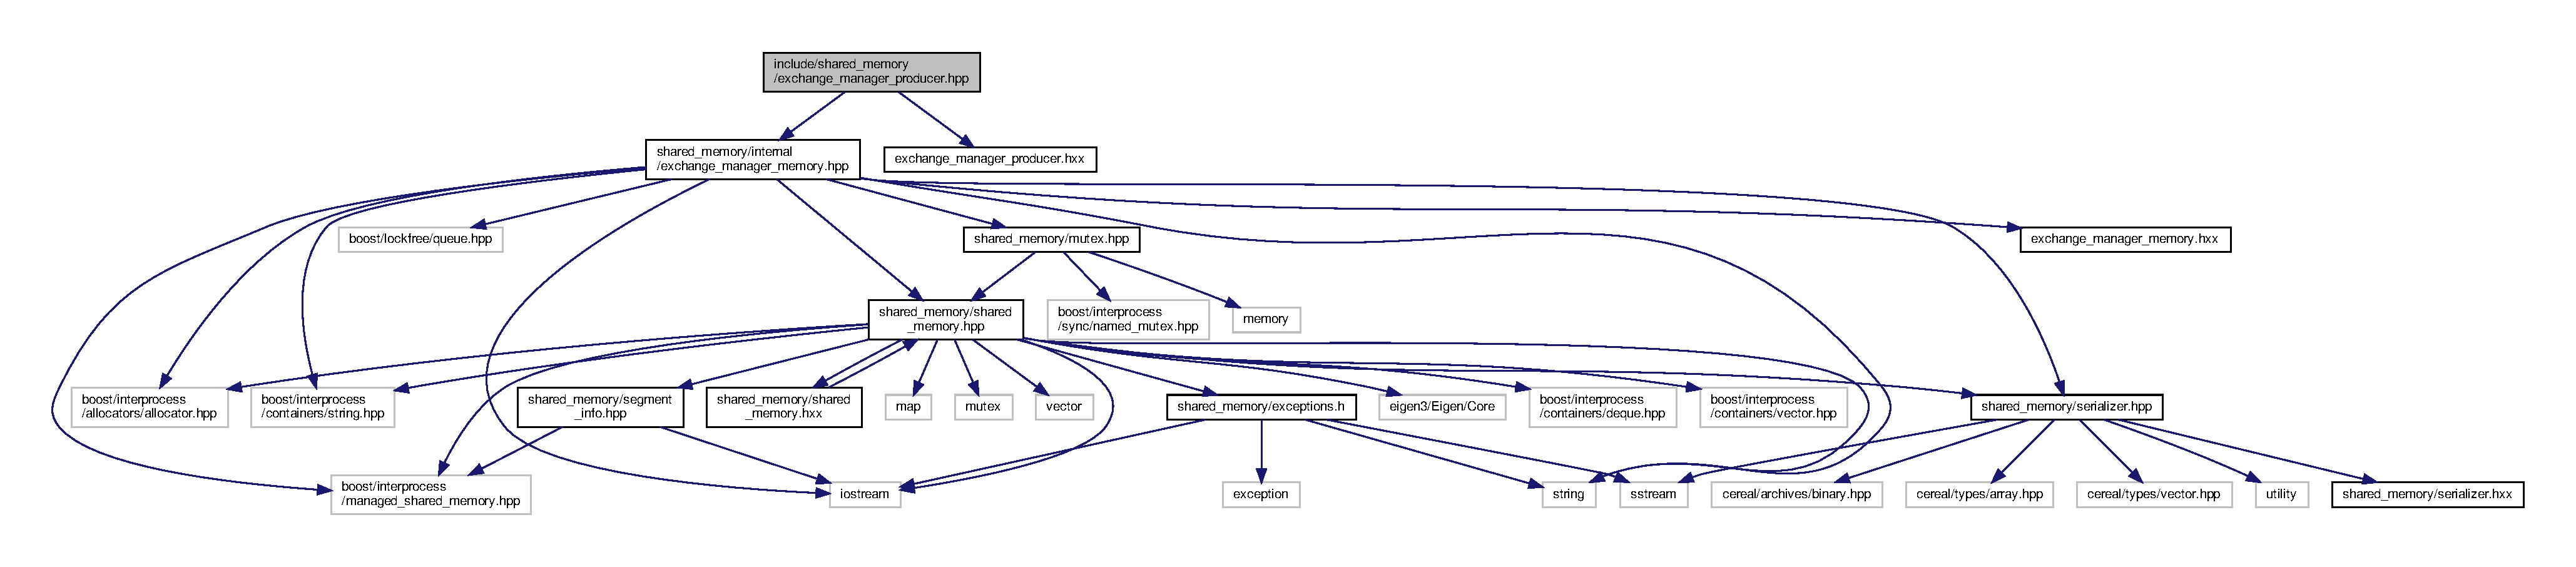
\includegraphics[width=350pt]{exchange__manager__producer_8hpp__incl}
\end{center}
\end{figure}
This graph shows which files directly or indirectly include this file\+:
\nopagebreak
\begin{figure}[H]
\begin{center}
\leavevmode
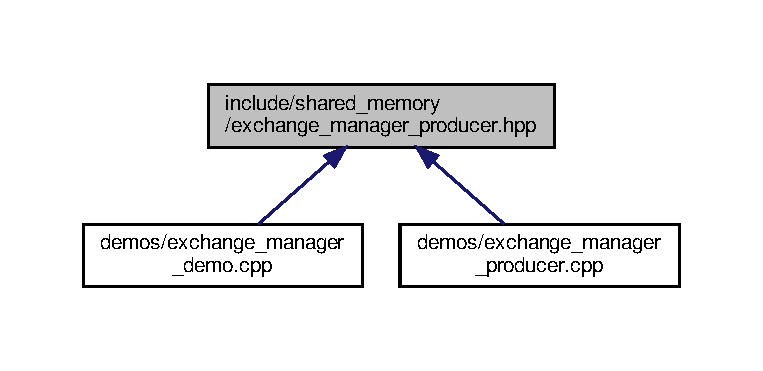
\includegraphics[width=350pt]{exchange__manager__producer_8hpp__dep__incl}
\end{center}
\end{figure}
\subsection*{Classes}
\begin{DoxyCompactItemize}
\item 
class \hyperlink{classshared__memory_1_1Exchange__manager__producer}{shared\+\_\+memory\+::\+Exchange\+\_\+manager\+\_\+producer$<$ Serializable, Q\+U\+E\+U\+E\+\_\+\+S\+I\+Z\+E $>$}
\end{DoxyCompactItemize}
\subsection*{Namespaces}
\begin{DoxyCompactItemize}
\item 
 \hyperlink{namespaceshared__memory}{shared\+\_\+memory}
\begin{DoxyCompactList}\small\item\em All templated types in this namespaces are elementary types\+: int, double, float, char$\ast$, ... \end{DoxyCompactList}\end{DoxyCompactItemize}


\subsection{Detailed Description}
Interprocess exchange of serialized items. 

\begin{DoxyAuthor}{Author}
Vincent Berenz (\href{mailto:vberenz@tuebingen.mpg.de}{\tt vberenz@tuebingen.\+mpg.\+de}) 
\end{DoxyAuthor}
\begin{DoxyRefDesc}{License}
\item[\hyperlink{license__license000022}{License}]License B\+S\+D-\/3-\/\+Clause \end{DoxyRefDesc}
\begin{DoxyCopyright}{Copyright}
Copyright (c) 2019, New York University and Max Planck Gesellschaft. 
\end{DoxyCopyright}
\begin{DoxyDate}{Date}
2019-\/06-\/07 
\end{DoxyDate}

\hypertarget{serializable__exchange_8hpp}{}\section{include/shared\+\_\+memory/serializable\+\_\+exchange.hpp File Reference}
\label{serializable__exchange_8hpp}\index{include/shared\+\_\+memory/serializable\+\_\+exchange.\+hpp@{include/shared\+\_\+memory/serializable\+\_\+exchange.\+hpp}}


Interface to a serializable object.  


{\ttfamily \#include $<$cstring$>$}\\*
{\ttfamily \#include $<$deque$>$}\\*
{\ttfamily \#include $<$stdexcept$>$}\\*
{\ttfamily \#include $<$string$>$}\\*
{\ttfamily \#include \char`\"{}shared\+\_\+memory/serializable.\+hpp\char`\"{}}\\*
{\ttfamily \#include \char`\"{}shared\+\_\+memory/shared\+\_\+memory.\+hpp\char`\"{}}\\*
{\ttfamily \#include \char`\"{}serializable\+\_\+exchange.\+hxx\char`\"{}}\\*
Include dependency graph for serializable\+\_\+exchange.\+hpp\+:
\nopagebreak
\begin{figure}[H]
\begin{center}
\leavevmode
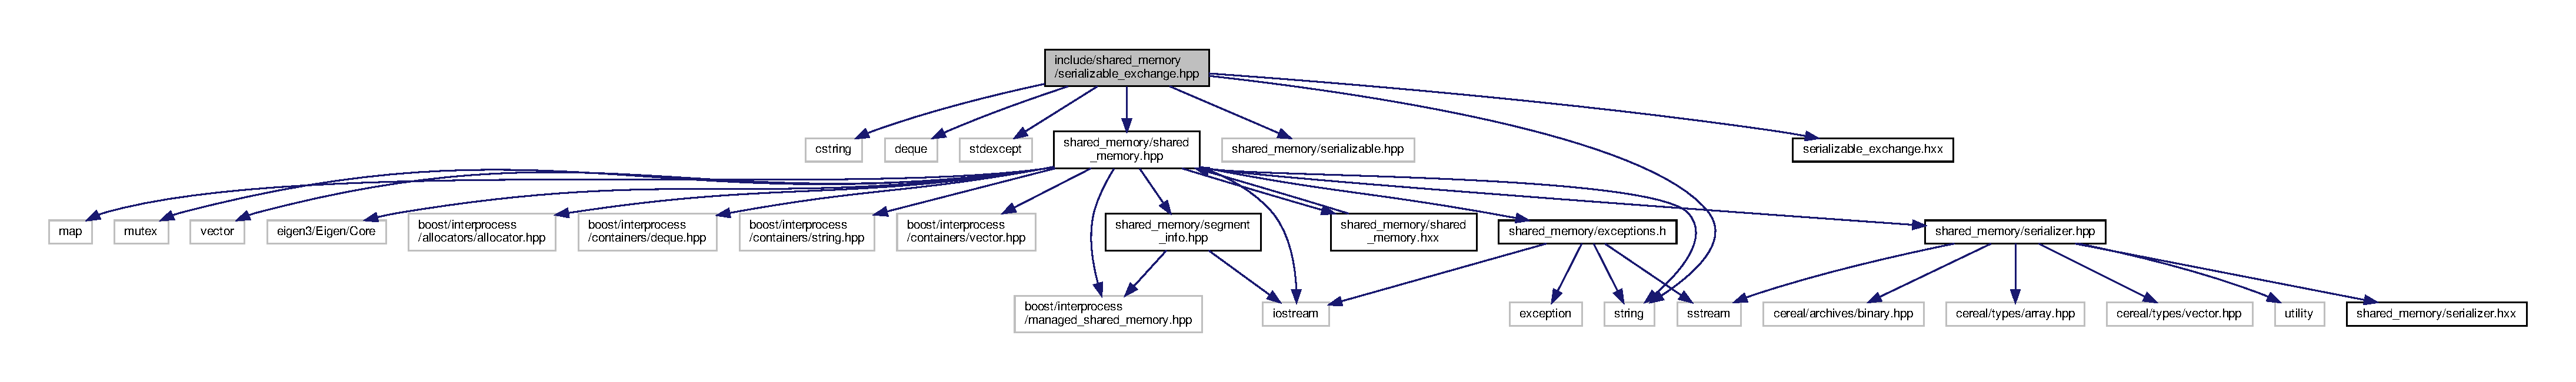
\includegraphics[width=350pt]{serializable__exchange_8hpp__incl}
\end{center}
\end{figure}
\subsection*{Classes}
\begin{DoxyCompactItemize}
\item 
class \hyperlink{classshared__memory_1_1Serializable__exchange}{shared\+\_\+memory\+::\+Serializable\+\_\+exchange$<$ Serializable $>$}
\end{DoxyCompactItemize}
\subsection*{Namespaces}
\begin{DoxyCompactItemize}
\item 
 \hyperlink{namespaceshared__memory}{shared\+\_\+memory}
\begin{DoxyCompactList}\small\item\em All templated types in this namespaces are elementary types\+: int, double, float, char$\ast$, ... \end{DoxyCompactList}\end{DoxyCompactItemize}


\subsection{Detailed Description}
Interface to a serializable object. 

\begin{DoxyAuthor}{Author}
Vincent Berenz 
\end{DoxyAuthor}
\begin{DoxyRefDesc}{License}
\item[\hyperlink{license__license000025}{License}]License B\+S\+D-\/3-\/\+Clause \end{DoxyRefDesc}
\begin{DoxyCopyright}{Copyright}
Copyright (c) 2019, New York University and Max Planck Gesellschaft. 
\end{DoxyCopyright}
\begin{DoxyDate}{Date}
2019-\/05-\/22 
\end{DoxyDate}

\hypertarget{serializable__exchange_8hxx}{}\section{include/shared\+\_\+memory/serializable\+\_\+exchange.hxx File Reference}
\label{serializable__exchange_8hxx}\index{include/shared\+\_\+memory/serializable\+\_\+exchange.\+hxx@{include/shared\+\_\+memory/serializable\+\_\+exchange.\+hxx}}


Define the template method of the Serializable\+\_\+exchange.  


This graph shows which files directly or indirectly include this file\+:
\nopagebreak
\begin{figure}[H]
\begin{center}
\leavevmode
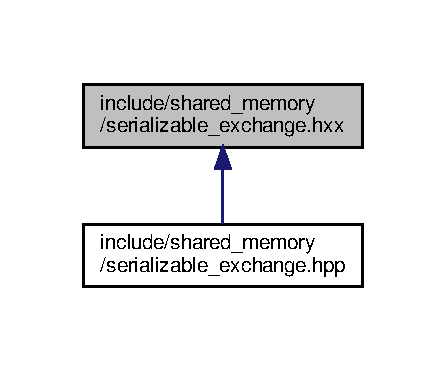
\includegraphics[width=214pt]{serializable__exchange_8hxx__dep__incl}
\end{center}
\end{figure}


\subsection{Detailed Description}
Define the template method of the Serializable\+\_\+exchange. 

\begin{DoxyAuthor}{Author}
Vincent Berenz 
\end{DoxyAuthor}
\begin{DoxyRefDesc}{License}
\item[\hyperlink{license__license000026}{License}]License B\+S\+D-\/3-\/\+Clause \end{DoxyRefDesc}
\begin{DoxyCopyright}{Copyright}
Copyright (c) 2019, New York University and Max Planck Gesellschaft. 
\end{DoxyCopyright}
\begin{DoxyDate}{Date}
2019-\/05-\/22
\end{DoxyDate}
\begin{DoxyAuthor}{Author}
Vincent Berenz 
\end{DoxyAuthor}
\begin{DoxyRefDesc}{License}
\item[\hyperlink{license__license000027}{License}]License B\+S\+D-\/3-\/\+Clause \end{DoxyRefDesc}
\begin{DoxyCopyright}{Copyright}
Copyright (c) 2019, New York University and Max Planck Gesellschaft. 
\end{DoxyCopyright}
\begin{DoxyDate}{Date}
2019-\/05-\/22 
\end{DoxyDate}

\hypertarget{shared__memory_8hpp}{}\section{include/shared\+\_\+memory/shared\+\_\+memory.hpp File Reference}
\label{shared__memory_8hpp}\index{include/shared\+\_\+memory/shared\+\_\+memory.\+hpp@{include/shared\+\_\+memory/shared\+\_\+memory.\+hpp}}


This file declares a class that is used for shared memory segment introspection (e.\+g. used and free memory)  


{\ttfamily \#include $<$iostream$>$}\newline
{\ttfamily \#include $<$map$>$}\newline
{\ttfamily \#include $<$mutex$>$}\newline
{\ttfamily \#include $<$string$>$}\newline
{\ttfamily \#include $<$vector$>$}\newline
{\ttfamily \#include $<$eigen3/\+Eigen/\+Core$>$}\newline
{\ttfamily \#include $<$boost/interprocess/allocators/allocator.\+hpp$>$}\newline
{\ttfamily \#include $<$boost/interprocess/containers/deque.\+hpp$>$}\newline
{\ttfamily \#include $<$boost/interprocess/containers/string.\+hpp$>$}\newline
{\ttfamily \#include $<$boost/interprocess/containers/vector.\+hpp$>$}\newline
{\ttfamily \#include $<$boost/interprocess/managed\+\_\+shared\+\_\+memory.\+hpp$>$}\newline
{\ttfamily \#include \char`\"{}shared\+\_\+memory/exceptions.\+h\char`\"{}}\newline
{\ttfamily \#include \char`\"{}shared\+\_\+memory/segment\+\_\+info.\+hpp\char`\"{}}\newline
{\ttfamily \#include \char`\"{}shared\+\_\+memory/serializer.\+hpp\char`\"{}}\newline
{\ttfamily \#include $<$shared\+\_\+memory/shared\+\_\+memory.\+hxx$>$}\newline
Include dependency graph for shared\+\_\+memory.\+hpp\+:
\nopagebreak
\begin{figure}[H]
\begin{center}
\leavevmode
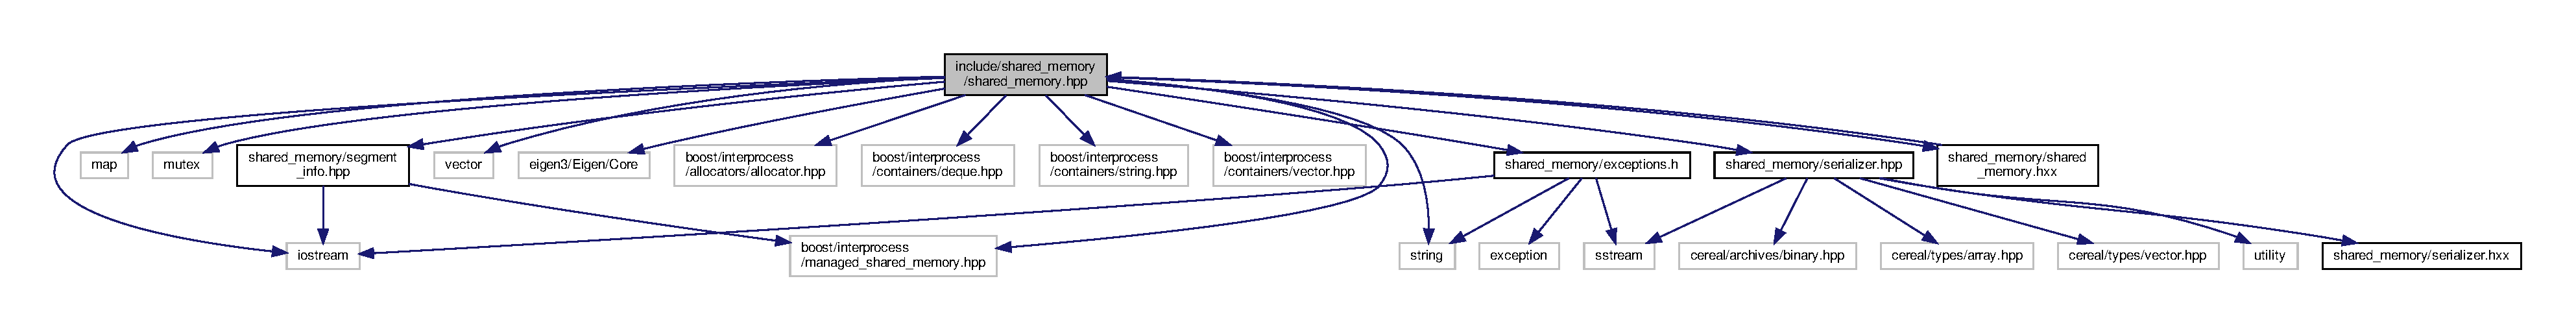
\includegraphics[width=350pt]{shared__memory_8hpp__incl}
\end{center}
\end{figure}
This graph shows which files directly or indirectly include this file\+:
\nopagebreak
\begin{figure}[H]
\begin{center}
\leavevmode
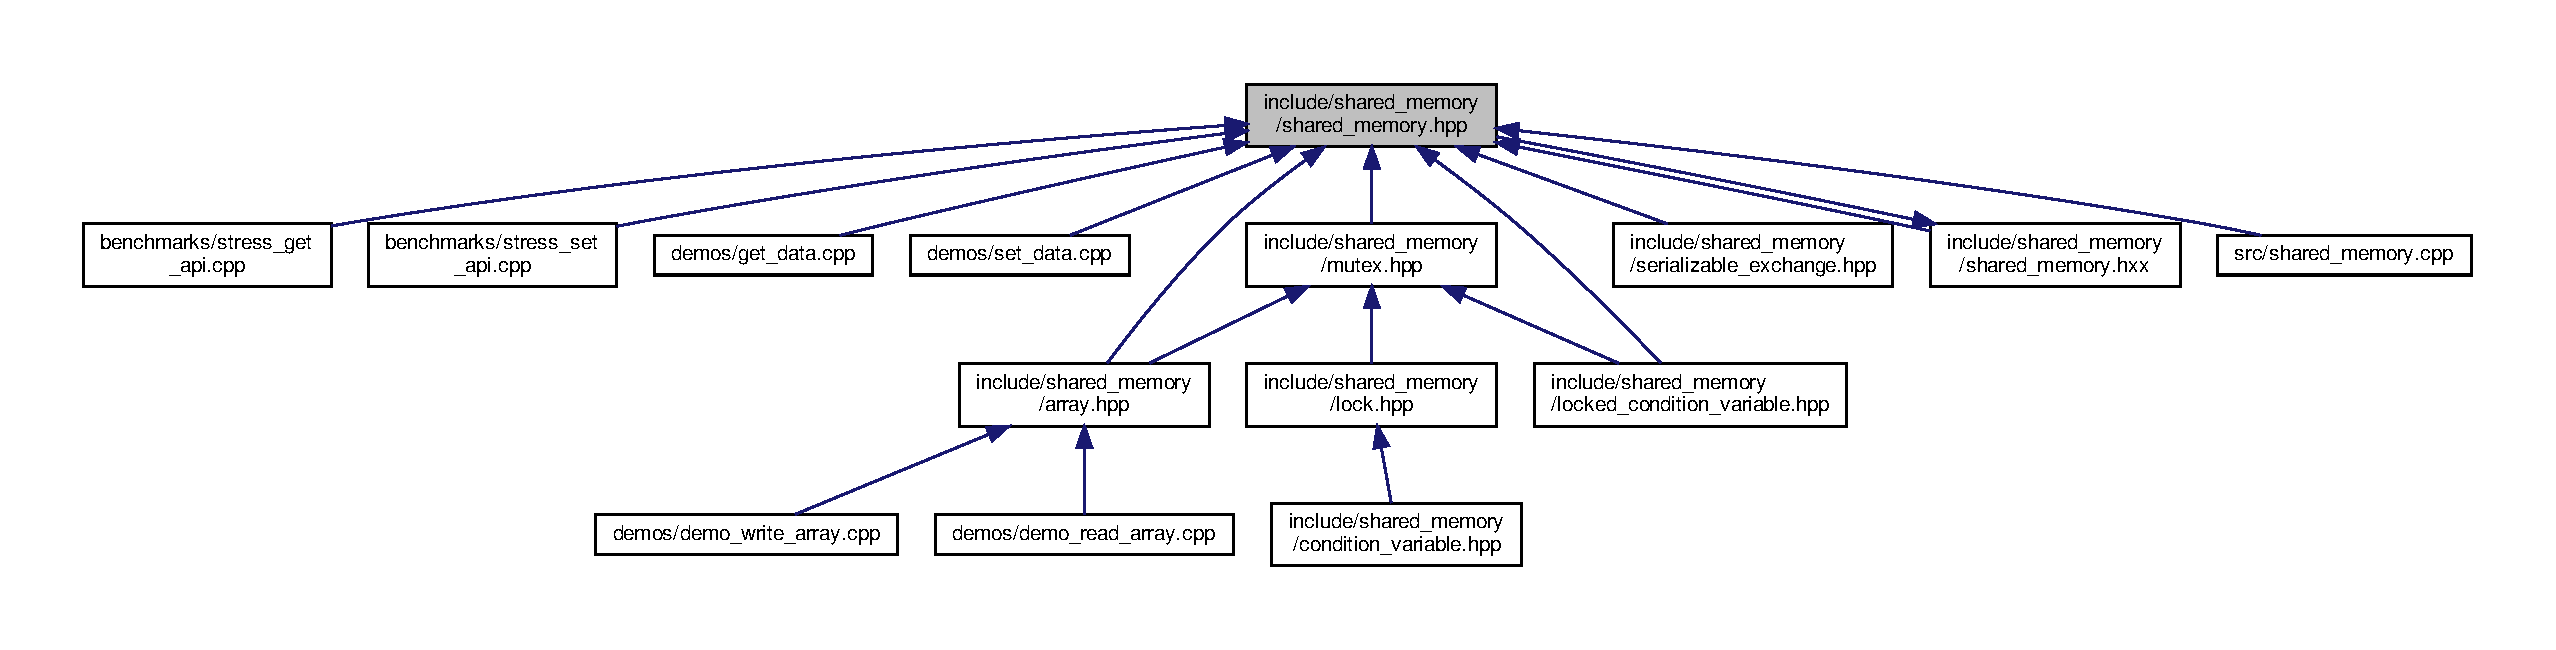
\includegraphics[width=350pt]{shared__memory_8hpp__dep__incl}
\end{center}
\end{figure}
\subsection*{Classes}
\begin{DoxyCompactItemize}
\item 
struct \hyperlink{structshared__memory_1_1ShmTypeHelper}{shared\+\_\+memory\+::\+Shm\+Type\+Helper$<$ Elem\+Type $>$}
\begin{DoxyCompactList}\small\item\em \hyperlink{structshared__memory_1_1ShmTypeHelper}{Shm\+Type\+Helper} is a small struct that allow the definition of templated typedef. \end{DoxyCompactList}\item 
class \hyperlink{classshared__memory_1_1SharedMemorySegment}{shared\+\_\+memory\+::\+Shared\+Memory\+Segment}
\begin{DoxyCompactList}\small\item\em The \hyperlink{classshared__memory_1_1SharedMemorySegment}{Shared\+Memory\+Segment} contains the pointers of the shared objects in on shared memrory segment. \end{DoxyCompactList}\end{DoxyCompactItemize}
\subsection*{Namespaces}
\begin{DoxyCompactItemize}
\item 
 \hyperlink{namespaceshared__memory}{shared\+\_\+memory}
\begin{DoxyCompactList}\small\item\em All templated types in this namespaces are elementary types\+: int, double, float, char$\ast$, ... \end{DoxyCompactList}\end{DoxyCompactItemize}
\subsection*{Macros}
\begin{DoxyCompactItemize}
\item 
\mbox{\Hypertarget{shared__memory_8hpp_af8fac614ab43478ad2a38d973f7ead6a}\label{shared__memory_8hpp_af8fac614ab43478ad2a38d973f7ead6a}} 
\#define {\bfseries S\+H\+A\+R\+E\+D\+\_\+\+M\+E\+M\+O\+R\+Y\+\_\+\+H\+PP}
\item 
\mbox{\Hypertarget{shared__memory_8hpp_acd2f5089f8d2870e833cdc9f7af461ec}\label{shared__memory_8hpp_acd2f5089f8d2870e833cdc9f7af461ec}} 
\#define {\bfseries D\+E\+F\+A\+U\+L\+T\+\_\+\+S\+H\+A\+R\+E\+D\+\_\+\+M\+E\+M\+O\+R\+Y\+\_\+\+S\+I\+ZE}~65536
\item 
\mbox{\Hypertarget{shared__memory_8hpp_af899411657e43cb548bc58ef7d88bec9}\label{shared__memory_8hpp_af899411657e43cb548bc58ef7d88bec9}} 
\#define {\bfseries M\+A\+P\+\_\+\+S\+T\+R\+I\+N\+G\+\_\+\+K\+E\+Y\+\_\+\+S\+E\+P\+A\+R\+A\+T\+OR}~\textquotesingle{};\textquotesingle{}
\end{DoxyCompactItemize}
\subsection*{Typedefs}
\begin{DoxyCompactItemize}
\item 
\mbox{\Hypertarget{namespaceshared__memory_ae50b2192256821112a69e47d5314b467}\label{namespaceshared__memory_ae50b2192256821112a69e47d5314b467}} 
typedef std\+::map$<$ std\+::string, std\+::pair$<$ void $\ast$, std\+::size\+\_\+t $>$ $>$ \hyperlink{namespaceshared__memory_ae50b2192256821112a69e47d5314b467}{shared\+\_\+memory\+::\+Shm\+Objects}
\begin{DoxyCompactList}\small\item\em Shm\+Objects typedef is a simple renaming that ease the for loop writting. \end{DoxyCompactList}\item 
\mbox{\Hypertarget{namespaceshared__memory_a36a105df63154c883e86f4282f380647}\label{namespaceshared__memory_a36a105df63154c883e86f4282f380647}} 
typedef Shm\+Type\+Helper$<$ char $>$\+::Elem\+Type\+Allocator \hyperlink{namespaceshared__memory_a36a105df63154c883e86f4282f380647}{shared\+\_\+memory\+::\+Shm\+Char\+Allocator}
\begin{DoxyCompactList}\small\item\em Create a char allocator to ease the creation of strings. \end{DoxyCompactList}\item 
\mbox{\Hypertarget{namespaceshared__memory_a07ee51d077030d33ba8408f5938569cc}\label{namespaceshared__memory_a07ee51d077030d33ba8408f5938569cc}} 
typedef std\+::basic\+\_\+string$<$ char, std\+::char\+\_\+traits$<$ char $>$, Shm\+Char\+Allocator $>$ \hyperlink{namespaceshared__memory_a07ee51d077030d33ba8408f5938569cc}{shared\+\_\+memory\+::\+Shm\+String}
\begin{DoxyCompactList}\small\item\em Create a basic\+\_\+string type for the Shared Memory. \end{DoxyCompactList}\end{DoxyCompactItemize}
\subsection*{Functions}
\begin{DoxyCompactItemize}
\item 
void \hyperlink{namespaceshared__memory_ac8ef94dc78f444092f488f0143b155f2}{shared\+\_\+memory\+::set\+\_\+segment\+\_\+sizes} (uint multiplier\+\_\+1025)
\begin{DoxyCompactList}\small\item\em sets the size of the segments that will be newly created via the set methods. \end{DoxyCompactList}\item 
\mbox{\Hypertarget{namespaceshared__memory_a841687861fcc9efe381ffbe84843ca33}\label{namespaceshared__memory_a841687861fcc9efe381ffbe84843ca33}} 
void \hyperlink{namespaceshared__memory_a841687861fcc9efe381ffbe84843ca33}{shared\+\_\+memory\+::set\+\_\+default\+\_\+segment\+\_\+sizes} ()
\begin{DoxyCompactList}\small\item\em set the size of segment newly created to the default size value of 65536 \end{DoxyCompactList}\item 
Shared\+Memory\+Segment \& \hyperlink{namespaceshared__memory_a7c76ec22ab70d3b7487becd3ec9943bc}{shared\+\_\+memory\+::get\+\_\+segment} (const std\+::string \&segment\+\_\+id, const bool clear\+\_\+upon\+\_\+destruction=false)
\begin{DoxyCompactList}\small\item\em get\+\_\+segment creates or give back a pointer to a \hyperlink{classshared__memory_1_1SharedMemorySegment}{Shared\+Memory\+Segment} object. \end{DoxyCompactList}\item 
Segment\+Info \hyperlink{namespaceshared__memory_a70f7613a247615e323cab083934c803e}{shared\+\_\+memory\+::get\+\_\+segment\+\_\+info} (const std\+::string \&segment\+\_\+id, const bool clear\+\_\+upon\+\_\+destruction=false)
\begin{DoxyCompactList}\small\item\em performs introspection on the segment and return related information. \end{DoxyCompactList}\item 
bool \hyperlink{namespaceshared__memory_a82297c2b7b85c57c53578749c9bd6429}{shared\+\_\+memory\+::segment\+\_\+exists} (const std\+::string \&segment\+\_\+id)
\begin{DoxyCompactList}\small\item\em returns true if a segment exists under this id \end{DoxyCompactList}\item 
void \hyperlink{namespaceshared__memory_a60cbce63ae7fb64a2758b773f9006471}{shared\+\_\+memory\+::delete\+\_\+segment} (const std\+::string \&segment\+\_\+id)
\begin{DoxyCompactList}\small\item\em delete\+\_\+segment deletes the segment of existing shared memory. \end{DoxyCompactList}\item 
\mbox{\Hypertarget{namespaceshared__memory_a1f88dd41dca9a23387090866213dbd85}\label{namespaceshared__memory_a1f88dd41dca9a23387090866213dbd85}} 
void \hyperlink{namespaceshared__memory_a1f88dd41dca9a23387090866213dbd85}{shared\+\_\+memory\+::delete\+\_\+all\+\_\+segment} ()
\begin{DoxyCompactList}\small\item\em delete\+\_\+all\+\_\+segment delete all mapping to the shared memory used during the current process \end{DoxyCompactList}\item 
{\footnotesize template$<$typename Elem\+Type $>$ }\\bool \hyperlink{namespaceshared__memory_a7b43b29fa0aa6a5cad0ca47afdd03e83}{shared\+\_\+memory\+::delete\+\_\+object} (const std\+::string \&segment\+\_\+id, const std\+::string \&object\+\_\+id)
\begin{DoxyCompactList}\small\item\em delete\+\_\+object deletes a particular object in the shared memory segment \end{DoxyCompactList}\item 
boost\+::interprocess\+::interprocess\+\_\+mutex \& \hyperlink{namespaceshared__memory_aed33c9701140a1c43e40f182a380199b}{shared\+\_\+memory\+::get\+\_\+segment\+\_\+mutex} (const std\+::string segment\+\_\+id)
\begin{DoxyCompactList}\small\item\em get\+\_\+sgement\+\_\+mutex aquiere a reference to the semgent global mutex. \end{DoxyCompactList}\item 
void \hyperlink{namespaceshared__memory_aa8583540879db53fc80b31410b5eec68}{shared\+\_\+memory\+::clear\+\_\+shared\+\_\+memory} (const std\+::string \&segment\+\_\+id)
\begin{DoxyCompactList}\small\item\em clear\+\_\+shared\+\_\+memory\+\_\+segment destroys the shared memory \end{DoxyCompactList}\item 
{\footnotesize template$<$typename Elem\+Type $>$ }\\void \hyperlink{namespaceshared__memory_ace68bf582cfe50ba83a9cfc9b7aed3b2}{shared\+\_\+memory\+::set} (const std\+::string \&segment\+\_\+id, const std\+::string \&object\+\_\+id, const Elem\+Type \&set\+\_\+)
\begin{DoxyCompactList}\small\item\em set instanciates or get pointer to any elementary types in the shared memory. \end{DoxyCompactList}\item 
{\footnotesize template$<$typename Elem\+Type $>$ }\\void \hyperlink{namespaceshared__memory_a7e37a0a2146d2cfeeccb63390a3d9132}{shared\+\_\+memory\+::set} (const std\+::string \&segment\+\_\+id, const std\+::string \&object\+\_\+id, const Elem\+Type $\ast$set\+\_\+, const std\+::size\+\_\+t size)
\begin{DoxyCompactList}\small\item\em set instanciates or get pointer to a fixed sized array of the templated type \char`\"{}\+T\char`\"{} in the shared memory. \end{DoxyCompactList}\item 
void \hyperlink{namespaceshared__memory_a61a2945c994bcbe84cc8dce96a189edb}{shared\+\_\+memory\+::set} (const std\+::string \&segment\+\_\+id, const std\+::string \&object\+\_\+id, const std\+::string \&set\+\_\+)
\begin{DoxyCompactList}\small\item\em set instanciates or get pointer to a string in the shared memory. \end{DoxyCompactList}\item 
{\footnotesize template$<$typename Elem\+Type $>$ }\\void \hyperlink{namespaceshared__memory_ac6521a6731fa97be21779b1d6c7589ee}{shared\+\_\+memory\+::set} (const std\+::string \&segment\+\_\+id, const std\+::string \&object\+\_\+id, const std\+::vector$<$ Elem\+Type $>$ \&set\+\_\+)
\begin{DoxyCompactList}\small\item\em set instanciates or get pointer to a std\+::vector$<$\+Elem\+Type$>$ in the shared memory. \end{DoxyCompactList}\item 
{\footnotesize template$<$typename Elem\+Type $>$ }\\void \hyperlink{namespaceshared__memory_ac8364e5cde6c8a2f1abc2a59035f26a6}{shared\+\_\+memory\+::set} (const std\+::string \&segment\+\_\+id, const std\+::string \&object\+\_\+id, const Eigen\+::\+Matrix$<$ Elem\+Type, Eigen\+::\+Dynamic, 1 $>$ \&set\+\_\+)
\begin{DoxyCompactList}\small\item\em set instanciates or get pointer to a Eigen\+::\+Matrix$<$\+Elem\+Type, Eigen\+::\+Dynamic, 1$>$ in the shared memory. \end{DoxyCompactList}\item 
{\footnotesize template$<$typename First\+Type , typename Second\+Type $>$ }\\void \hyperlink{namespaceshared__memory_a657bb799483a19a96f61706b50aca1e7}{shared\+\_\+memory\+::set} (const std\+::string \&segment\+\_\+id, const std\+::string \&object\+\_\+id, const std\+::pair$<$ First\+Type, Second\+Type $>$ \&set\+\_\+)
\begin{DoxyCompactList}\small\item\em set instanciates or get pointer to a std\+::pair$<$\+First\+Type, Second\+Type$>$ in the shared memory. \end{DoxyCompactList}\item 
{\footnotesize template$<$typename Key\+Type , typename Value\+Type $>$ }\\void \hyperlink{namespaceshared__memory_a562e79433e54463f39c9c276b8440f4b}{shared\+\_\+memory\+::set} (const std\+::string \&segment\+\_\+id, const std\+::string \&object\+\_\+id, const std\+::map$<$ Key\+Type, Value\+Type $>$ \&set\+\_\+)
\begin{DoxyCompactList}\small\item\em set instanciates or get pointer to a std\+::vector$<$\+Elem\+Type$>$ or an Eigen\+::\+Matrix$<$\+Elem\+Type, any, any$>$ in the shared memory. \end{DoxyCompactList}\item 
{\footnotesize template$<$typename Elem\+Type $>$ }\\void \hyperlink{namespaceshared__memory_ad017562102dbe044db2de6c79c0669d3}{shared\+\_\+memory\+::get} (const std\+::string \&segment\+\_\+id, const std\+::string \&object\+\_\+id, Elem\+Type \&get\+\_\+)
\begin{DoxyCompactList}\small\item\em get gets a pointer to any elementary types in the shared memory. \end{DoxyCompactList}\item 
{\footnotesize template$<$typename Elem\+Type $>$ }\\void \hyperlink{namespaceshared__memory_a6241b9143a2152b0c0beb784869373c7}{shared\+\_\+memory\+::get} (const std\+::string \&segment\+\_\+id, const std\+::string \&object\+\_\+id, Elem\+Type $\ast$get\+\_\+, const std\+::size\+\_\+t expected\+\_\+size)
\begin{DoxyCompactList}\small\item\em get gets a pointer to a fixed sized array of the templated type \char`\"{}\+T\char`\"{} in the shared memory. \end{DoxyCompactList}\item 
void \hyperlink{namespaceshared__memory_a8a952cc446e3dce8fea8cd1ea02613f9}{shared\+\_\+memory\+::get} (const std\+::string \&segment\+\_\+id, const std\+::string \&object\+\_\+id, std\+::string \&get\+\_\+)
\begin{DoxyCompactList}\small\item\em get gets a pointer to a string in the shared memory. \end{DoxyCompactList}\item 
{\footnotesize template$<$typename Elem\+Type $>$ }\\void \hyperlink{namespaceshared__memory_afd0ab66344562f5d927dea0d319a6a08}{shared\+\_\+memory\+::get} (const std\+::string \&segment\+\_\+id, const std\+::string \&object\+\_\+id, std\+::vector$<$ Elem\+Type $>$ \&get\+\_\+)
\begin{DoxyCompactList}\small\item\em get gets a pointer to a std\+::vector$<$\+Elem\+Type$>$ in the shared memory. \end{DoxyCompactList}\item 
{\footnotesize template$<$typename Elem\+Type $>$ }\\void \hyperlink{namespaceshared__memory_a4e230e55e38089aee71cd6df93110174}{shared\+\_\+memory\+::get} (const std\+::string \&segment\+\_\+id, const std\+::string \&object\+\_\+id, Eigen\+::\+Matrix$<$ Elem\+Type, Eigen\+::\+Dynamic, 1 $>$ \&get\+\_\+)
\begin{DoxyCompactList}\small\item\em get gets a pointer to a Eigen\+::\+Matrix$<$\+Elem\+Type, Eigen\+::\+Dynamic, 1$>$ in the shared memory. \end{DoxyCompactList}\item 
{\footnotesize template$<$typename First\+Type , typename Second\+Type $>$ }\\void \hyperlink{namespaceshared__memory_a2579e9a10a16e0fbd006900c618addc8}{shared\+\_\+memory\+::get} (const std\+::string \&segment\+\_\+id, const std\+::string \&object\+\_\+id, std\+::pair$<$ First\+Type, Second\+Type $>$ \&get\+\_\+)
\begin{DoxyCompactList}\small\item\em get instanciates or get pointer to a std\+::pair$<$\+First\+Type, Second\+Type$>$ in the shared memory. \end{DoxyCompactList}\item 
{\footnotesize template$<$typename Key\+Type , typename Value\+Type $>$ }\\void \hyperlink{namespaceshared__memory_add6604c2716e51cdcf17de2439251089}{shared\+\_\+memory\+::get} (const std\+::string \&segment\+\_\+id, const std\+::string \&object\+\_\+id, std\+::map$<$ Key\+Type, Value\+Type $>$ \&get\+\_\+)
\begin{DoxyCompactList}\small\item\em get gets a pointer to a std\+::vector$<$\+Elem\+Type$>$ or an Eigen\+::\+Matrix$<$\+Elem\+Type, any, any$>$ in the shared memory. \end{DoxyCompactList}\item 
{\footnotesize template$<$class Serializable $>$ }\\void \hyperlink{namespaceshared__memory_a003005dc269ebf79f08523dc0f8d1ed0}{shared\+\_\+memory\+::serialize} (const std\+::string \&segment, const std\+::string \&object, const \hyperlink{classSerializable}{Serializable} \&serializable)
\begin{DoxyCompactList}\small\item\em Serialize the instance into a string which is written in the shared memory. \end{DoxyCompactList}\item 
{\footnotesize template$<$class Serializable $>$ }\\void \hyperlink{namespaceshared__memory_a33e39adccccefb603e2dafc7ea8733e8}{shared\+\_\+memory\+::deserialize} (const std\+::string \&segment, const std\+::string \&object, \hyperlink{classSerializable}{Serializable} \&serializable)
\begin{DoxyCompactList}\small\item\em Read from the memory a string that is deserialized into the passed instance of \hyperlink{classSerializable}{Serializable}. \end{DoxyCompactList}\item 
void \hyperlink{namespaceshared__memory_afe26d531f043f59bb36ea7816b8a40bf}{shared\+\_\+memory\+::set\+\_\+verbose} (bool mode)
\begin{DoxyCompactList}\small\item\em if verbose mode set to true (starting default is false), informaton about newly created objects will be displayed in the terminal. \end{DoxyCompactList}\end{DoxyCompactItemize}


\subsection{Detailed Description}
This file declares a class that is used for shared memory segment introspection (e.\+g. used and free memory) 

This file declares some function that encapsulate the use of the shared memory using the boost\+::interprocess package. usage\+: see demos and unit tests and documentation.

\begin{DoxyAuthor}{Author}
Vincent Berenz 

Maximilien Naveau (\href{mailto:maximilien.naveau@gmail.com}{\tt maximilien.\+naveau@gmail.\+com}) 
\end{DoxyAuthor}
\begin{DoxyRefDesc}{License}
\item[\hyperlink{license__license000023}{License}]License B\+S\+D-\/3-\/\+Clause \end{DoxyRefDesc}
\begin{DoxyCopyright}{Copyright}
Copyright (c) 2019, New York University and Max Planck Gesellschaft. 
\end{DoxyCopyright}
\begin{DoxyDate}{Date}
2019-\/05-\/22
\end{DoxyDate}
\begin{DoxyAuthor}{Author}
Vincent Berenz 

Maximilien Naveau (\href{mailto:maximilien.naveau@gmail.com}{\tt maximilien.\+naveau@gmail.\+com}) 
\end{DoxyAuthor}
\begin{DoxyRefDesc}{License}
\item[\hyperlink{license__license000027}{License}]License B\+S\+D-\/3-\/\+Clause \end{DoxyRefDesc}
\begin{DoxyCopyright}{Copyright}
Copyright (c) 2019, New York University and Max Planck Gesellschaft. 
\end{DoxyCopyright}
\begin{DoxyDate}{Date}
2019-\/05-\/22 
\end{DoxyDate}

\hypertarget{shared__memory_8hxx}{}\section{include/shared\+\_\+memory/shared\+\_\+memory.hxx File Reference}
\label{shared__memory_8hxx}\index{include/shared\+\_\+memory/shared\+\_\+memory.\+hxx@{include/shared\+\_\+memory/shared\+\_\+memory.\+hxx}}


This file implements the functions from \hyperlink{shared__memory_8hpp}{shared\+\_\+memory.\+hpp} that encapsulate the use of the shared memory using the boost\+::interprocess package. usage\+: see demos and unit tests and documentation.  


{\ttfamily \#include $<$shared\+\_\+memory/shared\+\_\+memory.\+hpp$>$}\newline
Include dependency graph for shared\+\_\+memory.\+hxx\+:
\nopagebreak
\begin{figure}[H]
\begin{center}
\leavevmode
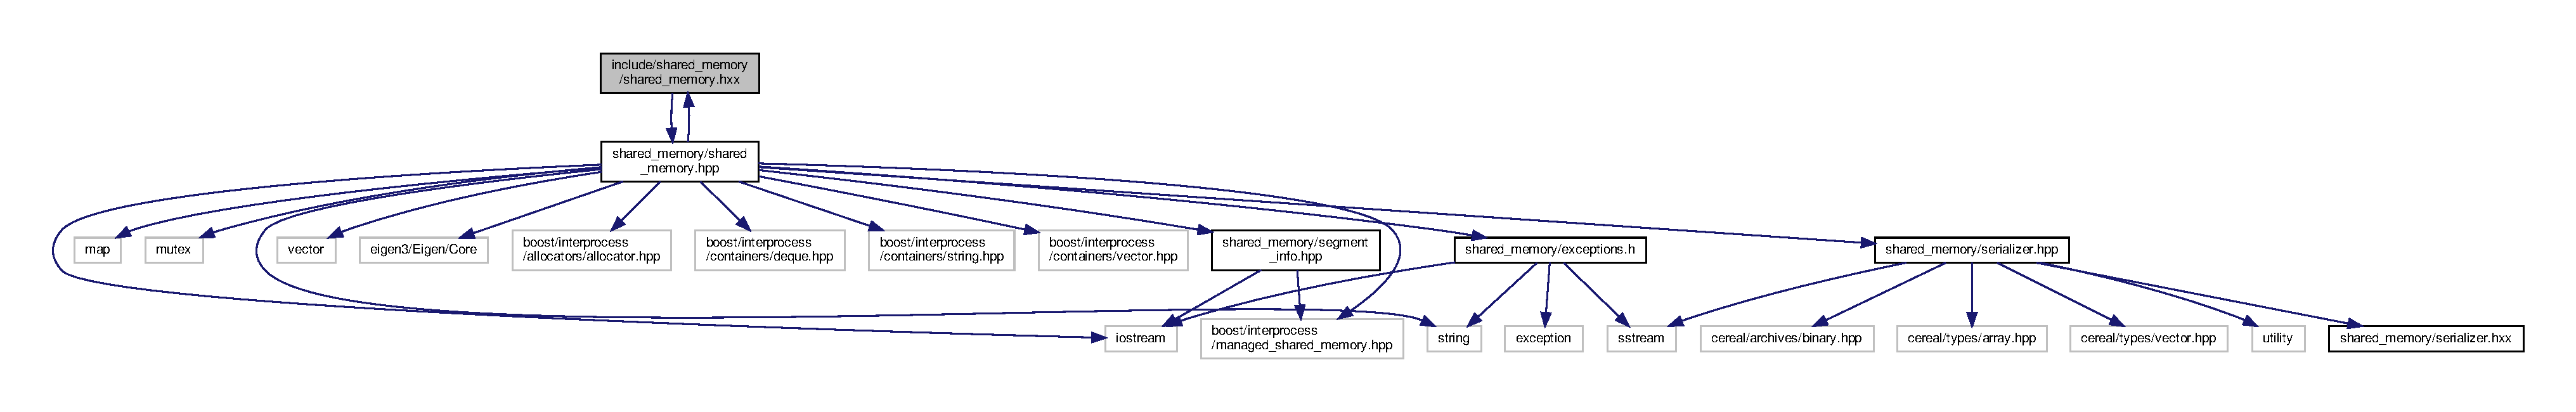
\includegraphics[width=350pt]{shared__memory_8hxx__incl}
\end{center}
\end{figure}
This graph shows which files directly or indirectly include this file\+:
\nopagebreak
\begin{figure}[H]
\begin{center}
\leavevmode
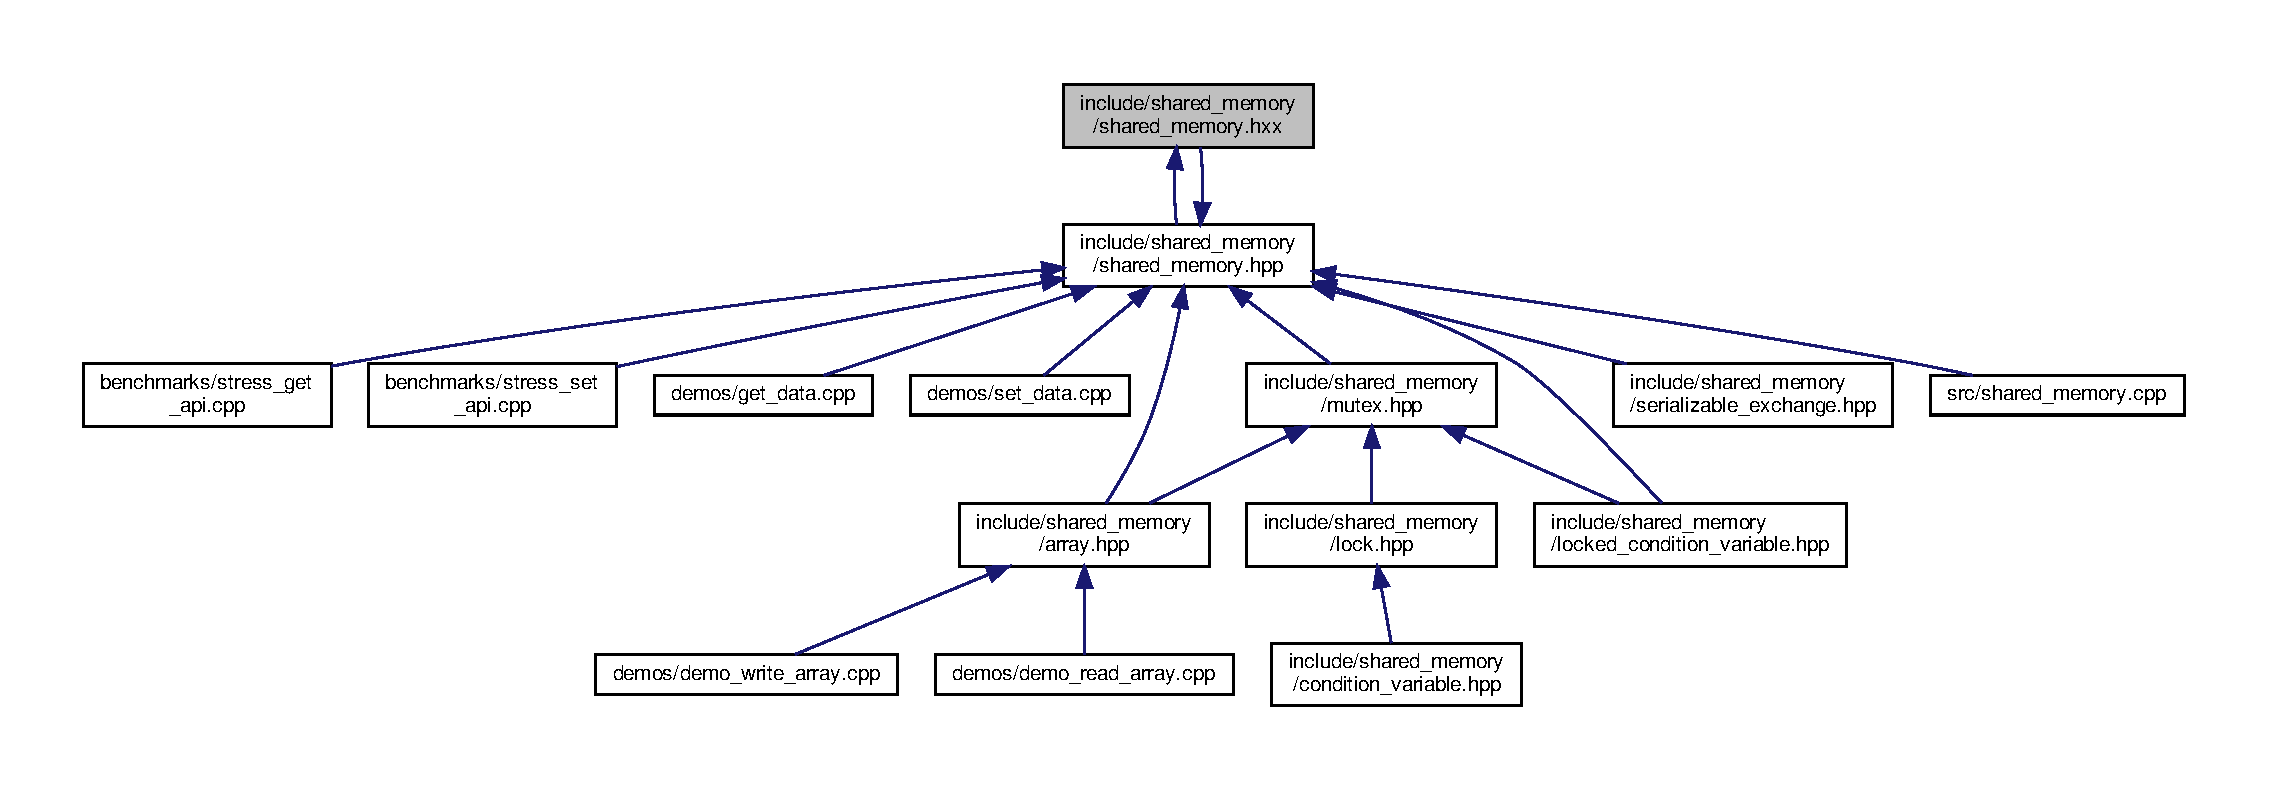
\includegraphics[width=350pt]{shared__memory_8hxx__dep__incl}
\end{center}
\end{figure}
\subsection*{Namespaces}
\begin{DoxyCompactItemize}
\item 
 \hyperlink{namespaceshared__memory}{shared\+\_\+memory}
\begin{DoxyCompactList}\small\item\em All templated types in this namespaces are elementary types\+: int, double, float, char$\ast$, ... \end{DoxyCompactList}\end{DoxyCompactItemize}
\subsection*{Typedefs}
\begin{DoxyCompactItemize}
\item 
\mbox{\Hypertarget{namespaceshared__memory_a9aeebdfb6185497cac7c093cf3d765c5}\label{namespaceshared__memory_a9aeebdfb6185497cac7c093cf3d765c5}} 
typedef std\+::map$<$ std\+::string, std\+::unique\+\_\+ptr$<$ Shared\+Memory\+Segment $>$ $>$ \hyperlink{namespaceshared__memory_a9aeebdfb6185497cac7c093cf3d765c5}{shared\+\_\+memory\+::\+Segment\+Map}
\begin{DoxyCompactList}\small\item\em Segment\+Map typedef is a simple short cut to the G\+L\+O\+B\+A\+L\+\_\+\+S\+H\+M\+\_\+\+S\+E\+G\+M\+E\+N\+TS type. \end{DoxyCompactList}\end{DoxyCompactItemize}
\subsection*{Functions}
\begin{DoxyCompactItemize}
\item 
{\footnotesize template$<$typename Elem\+Type $>$ }\\bool \hyperlink{namespaceshared__memory_a7b43b29fa0aa6a5cad0ca47afdd03e83}{shared\+\_\+memory\+::delete\+\_\+object} (const std\+::string \&segment\+\_\+id, const std\+::string \&object\+\_\+id)
\begin{DoxyCompactList}\small\item\em delete\+\_\+object deletes a particular object in the shared memory segment \end{DoxyCompactList}\item 
{\footnotesize template$<$typename Elem\+Type $>$ }\\void \hyperlink{namespaceshared__memory_ace68bf582cfe50ba83a9cfc9b7aed3b2}{shared\+\_\+memory\+::set} (const std\+::string \&segment\+\_\+id, const std\+::string \&object\+\_\+id, const Elem\+Type \&set\+\_\+)
\begin{DoxyCompactList}\small\item\em set instanciates or get pointer to any elementary types in the shared memory. \end{DoxyCompactList}\item 
{\footnotesize template$<$typename Elem\+Type $>$ }\\void \hyperlink{namespaceshared__memory_a7e37a0a2146d2cfeeccb63390a3d9132}{shared\+\_\+memory\+::set} (const std\+::string \&segment\+\_\+id, const std\+::string \&object\+\_\+id, const Elem\+Type $\ast$set\+\_\+, const std\+::size\+\_\+t size)
\begin{DoxyCompactList}\small\item\em set instanciates or get pointer to a fixed sized array of the templated type \char`\"{}\+T\char`\"{} in the shared memory. \end{DoxyCompactList}\item 
\mbox{\Hypertarget{namespaceshared__memory_a653947408c221da4e2c26439ba913f8d}\label{namespaceshared__memory_a653947408c221da4e2c26439ba913f8d}} 
{\footnotesize template$<$typename Vector\+Type , typename Elem\+Type $>$ }\\void {\bfseries shared\+\_\+memory\+::set} (const std\+::string \&segment\+\_\+id, const std\+::string \&object\+\_\+id, const Vector\+Type \&set\+\_\+)
\item 
{\footnotesize template$<$typename Elem\+Type $>$ }\\void \hyperlink{namespaceshared__memory_ac6521a6731fa97be21779b1d6c7589ee}{shared\+\_\+memory\+::set} (const std\+::string \&segment\+\_\+id, const std\+::string \&object\+\_\+id, const std\+::vector$<$ Elem\+Type $>$ \&set\+\_\+)
\begin{DoxyCompactList}\small\item\em set instanciates or get pointer to a std\+::vector$<$\+Elem\+Type$>$ in the shared memory. \end{DoxyCompactList}\item 
{\footnotesize template$<$typename Elem\+Type $>$ }\\void \hyperlink{namespaceshared__memory_ac8364e5cde6c8a2f1abc2a59035f26a6}{shared\+\_\+memory\+::set} (const std\+::string \&segment\+\_\+id, const std\+::string \&object\+\_\+id, const Eigen\+::\+Matrix$<$ Elem\+Type, Eigen\+::\+Dynamic, 1 $>$ \&set\+\_\+)
\begin{DoxyCompactList}\small\item\em set instanciates or get pointer to a Eigen\+::\+Matrix$<$\+Elem\+Type, Eigen\+::\+Dynamic, 1$>$ in the shared memory. \end{DoxyCompactList}\item 
{\footnotesize template$<$typename First\+Type , typename Second\+Type $>$ }\\void \hyperlink{namespaceshared__memory_a657bb799483a19a96f61706b50aca1e7}{shared\+\_\+memory\+::set} (const std\+::string \&segment\+\_\+id, const std\+::string \&object\+\_\+id, const std\+::pair$<$ First\+Type, Second\+Type $>$ \&set\+\_\+)
\begin{DoxyCompactList}\small\item\em set instanciates or get pointer to a std\+::pair$<$\+First\+Type, Second\+Type$>$ in the shared memory. \end{DoxyCompactList}\item 
{\footnotesize template$<$typename Key\+Type , typename Value\+Type $>$ }\\void \hyperlink{namespaceshared__memory_a562e79433e54463f39c9c276b8440f4b}{shared\+\_\+memory\+::set} (const std\+::string \&segment\+\_\+id, const std\+::string \&object\+\_\+id, const std\+::map$<$ Key\+Type, Value\+Type $>$ \&set\+\_\+)
\begin{DoxyCompactList}\small\item\em set instanciates or get pointer to a std\+::vector$<$\+Elem\+Type$>$ or an Eigen\+::\+Matrix$<$\+Elem\+Type, any, any$>$ in the shared memory. \end{DoxyCompactList}\item 
{\footnotesize template$<$typename Elem\+Type $>$ }\\void \hyperlink{namespaceshared__memory_ad017562102dbe044db2de6c79c0669d3}{shared\+\_\+memory\+::get} (const std\+::string \&segment\+\_\+id, const std\+::string \&object\+\_\+id, Elem\+Type \&get\+\_\+)
\begin{DoxyCompactList}\small\item\em get gets a pointer to any elementary types in the shared memory. \end{DoxyCompactList}\item 
{\footnotesize template$<$typename Elem\+Type $>$ }\\void \hyperlink{namespaceshared__memory_a6241b9143a2152b0c0beb784869373c7}{shared\+\_\+memory\+::get} (const std\+::string \&segment\+\_\+id, const std\+::string \&object\+\_\+id, Elem\+Type $\ast$get\+\_\+, const std\+::size\+\_\+t expected\+\_\+size)
\begin{DoxyCompactList}\small\item\em get gets a pointer to a fixed sized array of the templated type \char`\"{}\+T\char`\"{} in the shared memory. \end{DoxyCompactList}\item 
{\footnotesize template$<$typename Elem\+Type $>$ }\\void \hyperlink{namespaceshared__memory_afd0ab66344562f5d927dea0d319a6a08}{shared\+\_\+memory\+::get} (const std\+::string \&segment\+\_\+id, const std\+::string \&object\+\_\+id, std\+::vector$<$ Elem\+Type $>$ \&get\+\_\+)
\begin{DoxyCompactList}\small\item\em get gets a pointer to a std\+::vector$<$\+Elem\+Type$>$ in the shared memory. \end{DoxyCompactList}\item 
{\footnotesize template$<$typename Elem\+Type $>$ }\\void \hyperlink{namespaceshared__memory_a4e230e55e38089aee71cd6df93110174}{shared\+\_\+memory\+::get} (const std\+::string \&segment\+\_\+id, const std\+::string \&object\+\_\+id, Eigen\+::\+Matrix$<$ Elem\+Type, Eigen\+::\+Dynamic, 1 $>$ \&get\+\_\+)
\begin{DoxyCompactList}\small\item\em get gets a pointer to a Eigen\+::\+Matrix$<$\+Elem\+Type, Eigen\+::\+Dynamic, 1$>$ in the shared memory. \end{DoxyCompactList}\item 
{\footnotesize template$<$typename First\+Type , typename Second\+Type $>$ }\\void \hyperlink{namespaceshared__memory_a2579e9a10a16e0fbd006900c618addc8}{shared\+\_\+memory\+::get} (const std\+::string \&segment\+\_\+id, const std\+::string \&object\+\_\+id, std\+::pair$<$ First\+Type, Second\+Type $>$ \&get\+\_\+)
\begin{DoxyCompactList}\small\item\em get instanciates or get pointer to a std\+::pair$<$\+First\+Type, Second\+Type$>$ in the shared memory. \end{DoxyCompactList}\item 
{\footnotesize template$<$typename Key\+Type , typename Value\+Type $>$ }\\void \hyperlink{namespaceshared__memory_add6604c2716e51cdcf17de2439251089}{shared\+\_\+memory\+::get} (const std\+::string \&segment\+\_\+id, const std\+::string \&object\+\_\+id, std\+::map$<$ Key\+Type, Value\+Type $>$ \&get\+\_\+)
\begin{DoxyCompactList}\small\item\em get gets a pointer to a std\+::vector$<$\+Elem\+Type$>$ or an Eigen\+::\+Matrix$<$\+Elem\+Type, any, any$>$ in the shared memory. \end{DoxyCompactList}\end{DoxyCompactItemize}
\subsection*{Variables}
\begin{DoxyCompactItemize}
\item 
\mbox{\Hypertarget{namespaceshared__memory_adb7d7158652e09188fea583e05949bb5}\label{namespaceshared__memory_adb7d7158652e09188fea583e05949bb5}} 
bool {\bfseries shared\+\_\+memory\+::\+V\+E\+R\+B\+O\+SE} = false
\item 
static Segment\+Map \hyperlink{namespaceshared__memory_ad1f78482aa062e165f37fd49e2e8f539}{shared\+\_\+memory\+::\+G\+L\+O\+B\+A\+L\+\_\+\+S\+H\+M\+\_\+\+S\+E\+G\+M\+E\+N\+TS}
\begin{DoxyCompactList}\small\item\em G\+L\+O\+B\+A\+L\+\_\+\+S\+H\+A\+R\+E\+D\+\_\+\+M\+E\+M\+O\+R\+Y\+\_\+\+S\+E\+G\+M\+E\+NT is global variable that acts as a a shared memory manager. \end{DoxyCompactList}\end{DoxyCompactItemize}


\subsection{Detailed Description}
This file implements the functions from \hyperlink{shared__memory_8hpp}{shared\+\_\+memory.\+hpp} that encapsulate the use of the shared memory using the boost\+::interprocess package. usage\+: see demos and unit tests and documentation. 

\begin{DoxyAuthor}{Author}
Vincent Berenz 

Maximilien Naveau (\href{mailto:maximilien.naveau@gmail.com}{\tt maximilien.\+naveau@gmail.\+com}) 
\end{DoxyAuthor}
\begin{DoxyRefDesc}{License}
\item[\hyperlink{license__license000029}{License}]License B\+S\+D-\/3-\/\+Clause \end{DoxyRefDesc}
\begin{DoxyCopyright}{Copyright}
Copyright (c) 2019, New York University and Max Planck Gesellschaft. 
\end{DoxyCopyright}
\begin{DoxyDate}{Date}
2019-\/05-\/22 
\end{DoxyDate}

\hypertarget{exceptions_8cpp}{}\section{src/exceptions.cpp File Reference}
\label{exceptions_8cpp}\index{src/exceptions.\+cpp@{src/exceptions.\+cpp}}


Defines some exception specific to this A\+PI.  


{\ttfamily \#include \char`\"{}shared\+\_\+memory/exceptions.\+h\char`\"{}}\\*
Include dependency graph for exceptions.\+cpp\+:
\nopagebreak
\begin{figure}[H]
\begin{center}
\leavevmode
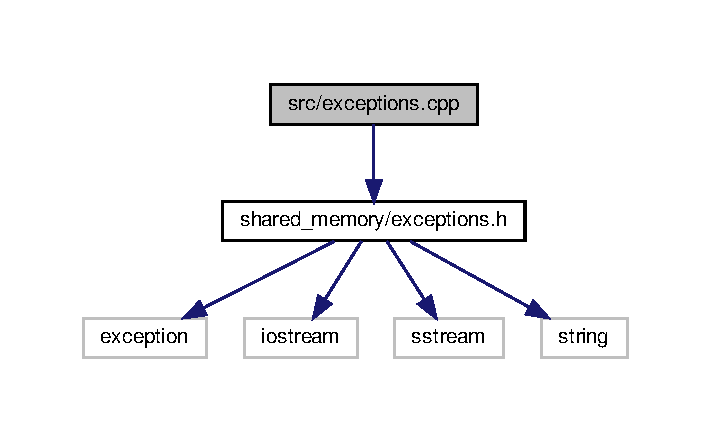
\includegraphics[width=341pt]{exceptions_8cpp__incl}
\end{center}
\end{figure}
\subsection*{Namespaces}
\begin{DoxyCompactItemize}
\item 
 \hyperlink{namespaceshared__memory}{shared\+\_\+memory}
\begin{DoxyCompactList}\small\item\em All templated types in this namespaces are elementary types\+: int, double, float, char$\ast$, ... \end{DoxyCompactList}\end{DoxyCompactItemize}


\subsection{Detailed Description}
Defines some exception specific to this A\+PI. 

\begin{DoxyAuthor}{Author}
Maximilien Naveau (\href{mailto:maximilien.naveau@gmail.com}{\tt maximilien.\+naveau@gmail.\+com}) 
\end{DoxyAuthor}
\begin{DoxyRefDesc}{License}
\item[\hyperlink{license__license000030}{License}]License B\+S\+D-\/3-\/\+Clause \end{DoxyRefDesc}
\begin{DoxyCopyright}{Copyright}
Copyright (c) 2019, New York University and Max Planck Gesellschaft. 
\end{DoxyCopyright}
\begin{DoxyDate}{Date}
2019-\/05-\/22 
\end{DoxyDate}

\hypertarget{shared__memory_8cpp}{}\section{src/shared\+\_\+memory.cpp File Reference}
\label{shared__memory_8cpp}\index{src/shared\+\_\+memory.\+cpp@{src/shared\+\_\+memory.\+cpp}}


Implementation of the \hyperlink{shared__memory_8hpp}{shared\+\_\+memory.\+hpp} A\+PI.  


{\ttfamily \#include \char`\"{}shared\+\_\+memory/shared\+\_\+memory.\+hpp\char`\"{}}\newline
Include dependency graph for shared\+\_\+memory.\+cpp\+:
\nopagebreak
\begin{figure}[H]
\begin{center}
\leavevmode
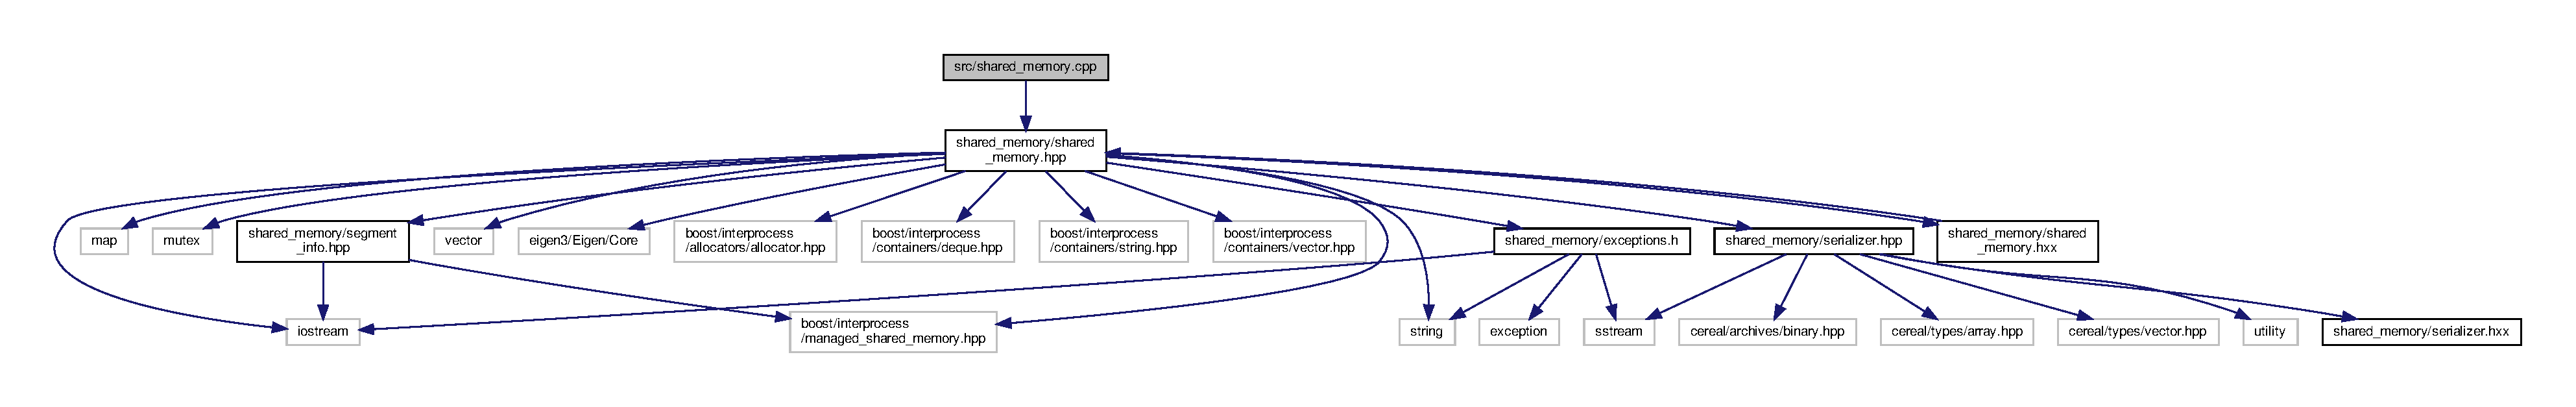
\includegraphics[width=350pt]{shared__memory_8cpp__incl}
\end{center}
\end{figure}
\subsection*{Namespaces}
\begin{DoxyCompactItemize}
\item 
 \hyperlink{namespaceshared__memory}{shared\+\_\+memory}
\begin{DoxyCompactList}\small\item\em All templated types in this namespaces are elementary types\+: int, double, float, char$\ast$, ... \end{DoxyCompactList}\end{DoxyCompactItemize}
\subsection*{Functions}
\begin{DoxyCompactItemize}
\item 
void \hyperlink{namespaceshared__memory_ac8ef94dc78f444092f488f0143b155f2}{shared\+\_\+memory\+::set\+\_\+segment\+\_\+sizes} (uint multiplier\+\_\+1025)
\begin{DoxyCompactList}\small\item\em sets the size of the segments that will be newly created via the set methods. \end{DoxyCompactList}\item 
\mbox{\Hypertarget{namespaceshared__memory_a841687861fcc9efe381ffbe84843ca33}\label{namespaceshared__memory_a841687861fcc9efe381ffbe84843ca33}} 
void \hyperlink{namespaceshared__memory_a841687861fcc9efe381ffbe84843ca33}{shared\+\_\+memory\+::set\+\_\+default\+\_\+segment\+\_\+sizes} ()
\begin{DoxyCompactList}\small\item\em set the size of segment newly created to the default size value of 65536 \end{DoxyCompactList}\item 
void \hyperlink{namespaceshared__memory_afe26d531f043f59bb36ea7816b8a40bf}{shared\+\_\+memory\+::set\+\_\+verbose} (bool mode)
\begin{DoxyCompactList}\small\item\em if verbose mode set to true (starting default is false), informaton about newly created objects will be displayed in the terminal. \end{DoxyCompactList}\item 
Shared\+Memory\+Segment \& \hyperlink{namespaceshared__memory_a7c76ec22ab70d3b7487becd3ec9943bc}{shared\+\_\+memory\+::get\+\_\+segment} (const std\+::string \&segment\+\_\+id, const bool clear\+\_\+upon\+\_\+destruction=false)
\begin{DoxyCompactList}\small\item\em get\+\_\+segment creates or give back a pointer to a \hyperlink{classshared__memory_1_1SharedMemorySegment}{Shared\+Memory\+Segment} object. \end{DoxyCompactList}\item 
Segment\+Info \hyperlink{namespaceshared__memory_a70f7613a247615e323cab083934c803e}{shared\+\_\+memory\+::get\+\_\+segment\+\_\+info} (const std\+::string \&segment\+\_\+id, const bool clear\+\_\+upon\+\_\+destruction=false)
\begin{DoxyCompactList}\small\item\em performs introspection on the segment and return related information. \end{DoxyCompactList}\item 
bool \hyperlink{namespaceshared__memory_a82297c2b7b85c57c53578749c9bd6429}{shared\+\_\+memory\+::segment\+\_\+exists} (const std\+::string \&segment\+\_\+id)
\begin{DoxyCompactList}\small\item\em returns true if a segment exists under this id \end{DoxyCompactList}\item 
boost\+::interprocess\+::interprocess\+\_\+mutex \& \hyperlink{namespaceshared__memory_aed33c9701140a1c43e40f182a380199b}{shared\+\_\+memory\+::get\+\_\+segment\+\_\+mutex} (const std\+::string segment\+\_\+id)
\begin{DoxyCompactList}\small\item\em get\+\_\+sgement\+\_\+mutex aquiere a reference to the semgent global mutex. \end{DoxyCompactList}\item 
void \hyperlink{namespaceshared__memory_a60cbce63ae7fb64a2758b773f9006471}{shared\+\_\+memory\+::delete\+\_\+segment} (const std\+::string \&segment\+\_\+id)
\begin{DoxyCompactList}\small\item\em delete\+\_\+segment deletes the segment of existing shared memory. \end{DoxyCompactList}\item 
\mbox{\Hypertarget{namespaceshared__memory_a1f88dd41dca9a23387090866213dbd85}\label{namespaceshared__memory_a1f88dd41dca9a23387090866213dbd85}} 
void \hyperlink{namespaceshared__memory_a1f88dd41dca9a23387090866213dbd85}{shared\+\_\+memory\+::delete\+\_\+all\+\_\+segment} ()
\begin{DoxyCompactList}\small\item\em delete\+\_\+all\+\_\+segment delete all mapping to the shared memory used during the current process \end{DoxyCompactList}\item 
void \hyperlink{namespaceshared__memory_aa8583540879db53fc80b31410b5eec68}{shared\+\_\+memory\+::clear\+\_\+shared\+\_\+memory} (const std\+::string \&segment\+\_\+id)
\begin{DoxyCompactList}\small\item\em clear\+\_\+shared\+\_\+memory\+\_\+segment destroys the shared memory \end{DoxyCompactList}\item 
void \hyperlink{namespaceshared__memory_a61a2945c994bcbe84cc8dce96a189edb}{shared\+\_\+memory\+::set} (const std\+::string \&segment\+\_\+id, const std\+::string \&object\+\_\+id, const std\+::string \&set\+\_\+)
\begin{DoxyCompactList}\small\item\em set instanciates or get pointer to a string in the shared memory. \end{DoxyCompactList}\item 
void \hyperlink{namespaceshared__memory_a8a952cc446e3dce8fea8cd1ea02613f9}{shared\+\_\+memory\+::get} (const std\+::string \&segment\+\_\+id, const std\+::string \&object\+\_\+id, std\+::string \&get\+\_\+)
\begin{DoxyCompactList}\small\item\em get gets a pointer to a string in the shared memory. \end{DoxyCompactList}\end{DoxyCompactItemize}
\subsection*{Variables}
\begin{DoxyCompactItemize}
\item 
\mbox{\Hypertarget{namespaceshared__memory_a1aa02b0b88f0045c3711029f882d80fa}\label{namespaceshared__memory_a1aa02b0b88f0045c3711029f882d80fa}} 
static uint {\bfseries shared\+\_\+memory\+::\+S\+E\+G\+M\+E\+N\+T\+\_\+\+S\+I\+ZE} = D\+E\+F\+A\+U\+L\+T\+\_\+\+S\+H\+A\+R\+E\+D\+\_\+\+M\+E\+M\+O\+R\+Y\+\_\+\+S\+I\+ZE
\item 
\mbox{\Hypertarget{namespaceshared__memory_a5c687b65860cde45c62305fbb7a19e71}\label{namespaceshared__memory_a5c687b65860cde45c62305fbb7a19e71}} 
static std\+::mutex {\bfseries shared\+\_\+memory\+::\+S\+E\+G\+M\+E\+N\+T\+\_\+\+S\+I\+Z\+E\+\_\+\+M\+U\+T\+EX}
\end{DoxyCompactItemize}


\subsection{Detailed Description}
Implementation of the \hyperlink{shared__memory_8hpp}{shared\+\_\+memory.\+hpp} A\+PI. 

\begin{DoxyAuthor}{Author}
Maximilien Naveau (\href{mailto:maximilien.naveau@gmail.com}{\tt maximilien.\+naveau@gmail.\+com}) 
\end{DoxyAuthor}
\begin{DoxyRefDesc}{License}
\item[\hyperlink{license__license000030}{License}]License B\+S\+D-\/3-\/\+Clause \end{DoxyRefDesc}
\begin{DoxyCopyright}{Copyright}
Copyright (c) 2019, New York University and Max Planck Gesellschaft. 
\end{DoxyCopyright}
\begin{DoxyDate}{Date}
2019-\/05-\/22 
\end{DoxyDate}

%--- End generated contents ---

% Index
\backmatter
\newpage
\phantomsection
\clearemptydoublepage
\addcontentsline{toc}{chapter}{Index}
\printindex

\end{document}
